\documentclass[chap]{thesis}

% geometry
% use option 'showframe' for neatness
\usepackage{geometry}
\geometry{
left=1in,
right=1in,
top=1in,
bottom=1in}

% citations
\usepackage{cite}
\usepackage{notoccite}
\bibliographystyle{IEEErpi}
\renewcommand{\bibname}{}

% captions
\usepackage[
  labelsep=period,
  justification=centering]{caption}
\usepackage{subcaption}

% put captions above tables
\usepackage{float}
\floatstyle{plaintop}
\restylefloat{table}

% COMMAT
\usepackage{textcomp}
\usepackage{float}
\usepackage{caption}
\usepackage{multirow}
\usepackage{booktabs}
\usepackage{tikz}
\usetikzlibrary{shapes,arrows}

\tikzstyle{line} = [thick,->,>=stealth]

%\tikzstyle{line} = [draw, -latex']
\tikzstyle{decision} = [diamond, draw, fill=green!30, 
    text width=10em, text badly centered, inner sep=0pt]
\tikzstyle{process} = [rectangle, draw, fill=orange!30, 
    text width=10em, text centered, rounded corners, minimum height=5em]
\tikzstyle{input} = [rectangle, draw, fill=blue!30, 
    text width=10em, text centered, rounded corners, minimum height=5em]
\tikzstyle{block} = [rectangle, draw, fill=none, 
    text width=10em, text centered, rounded corners, minimum height=5em]
\tikzstyle{line} = [draw, -latex']

\usepackage{adjustbox}
\usepackage[justification=centering]{caption}


% mathematics
\usepackage{amsmath}
\usepackage{amssymb}
\usepackage{amsthm}
\usepackage{mathrsfs}
\usepackage{upgreek}

% figures
\usepackage{graphicx}

% make things pretty
\usepackage{color}
\usepackage[hidelinks]{hyperref}

% make pretty graphs
\usepackage{tikz}
\usetikzlibrary{arrows}

% make pretty tables
\usepackage{tabu}

% algorithms
\usepackage{algpseudocode}
\usepackage{algorithm}
\usepackage{longtable}
% code listings
\usepackage{listings}
\lstdefinestyle{mystyle}{
  basicstyle=\ttfamily,
  language=C++,
  columns=fullflexible,
  keepspaces=true,
  numbers=left,
  xleftmargin=2em
}

% conform to IEEE
\renewcommand{\captionfont}{\bfseries}
\renewcommand{\figurename}{Fig.}
\renewcommand*{\UrlNoBreaks}{\do\(\do\[\do\{\do\<\do\:}%

% href for toc
\makeatletter
\usepackage{etoolbox}
\pretocmd{\tableofcontents}{%
  \if@openright\cleardoublepage\else\clearpage\fi
  \pdfbookmark[0]{\contentsname}{toc}%
}{}{}%
\makeatother

% theorems and propositions
\newtheorem{prop}{Proposition}
\theoremstyle{remark}
\newtheorem{rmk}{Remark}

% make typing easier
\newcommand{\B}{\mathcal{B}}
\newcommand{\E}{\mathcal{E}}
\newcommand{\G}{\mathcal{G}}
\newcommand{\I}{\mathcal{I}}
\newcommand{\J}{\mathcal{J}}
\newcommand{\R}{\mathcal{R}}
\newcommand{\V}{\mathcal{V}}
\newcommand{\OP}{\mathcal{L}}
\renewcommand{\H}{\mathcal{H}}
\renewcommand{\O}{\mathcal{O}}
\renewcommand{\P}{\mathcal{P}}
\renewcommand{\S}{\mathcal{S}}
\newcommand{\bs}[1]{\boldsymbol{#1}}

% make editors mad - keep my sanity
\renewcommand{\bar}[1]{\overline{#1}}
\renewcommand{\tilde}[1]{\widetilde{#1}}
\newcommand{\paira}[2]{\,{}_{\V^*}^{}\!\left< {#1}, {#2} \right>_{\V}}
\newcommand{\pairb}[2]{\,{}_{\V}^{}\!\left< {#1}, {#2} \right>_{\V^*}}
\newcommand{\adv}[1]{-\kappa \nabla^2 {#1} + \bs{a} \cdot \nabla {#1}}
\newcommand{\madv}[1]{\kappa \nabla^2 {#1} - \bs{a} \cdot \nabla {#1}}
\newcommand{\adva}[1]{-\kappa \nabla^2 {#1} - \bs{a} \cdot \nabla {#1}}
\newcommand{\madva}[1]{\kappa \nabla^2 {#1} + \bs{a} \cdot \nabla {#1}}

\begin{document}
\thesistitle{\bf Reducing image classification error and quantifying the contributions of components in a learning pipeline}

\author{Aritra Chowdhury}
\degree{Doctor of Philosophy}
\department{Computer Science}
\submitdate{[August 2018] \\ Submitted June 2018}
\copyrightyear{2018}

\titlepage
\copyrightpage
\tableofcontents
\listoftables
\listoffigures

\specialhead{ACKNOWLEDGMENT}

First and foremost, I would like to thank my advisor
Prof. Mark S. Shephard, for his guidance throughout my tenure
as a graduate student. Prof. Shephard's invaluable insights
and dedication to rigor and excellence have helped me become
a better researcher. I am honored to have been given the
opportunity to join his research group. I would also like
to thank my co-advisor, Prof. Assad A. Oberai, for his
insightful guidance and kindness.

I would like to thank Prof. Antionette M. Maniatty,
Prof. Jason E. Hicken, and Prof. Jeffrey W. Banks for
kindly serving on my doctoral committee, for the valuable
education they've provided me through their courses,
and for their helpfulness and willingness to answer questions
that arose during my time as a graduate student.

The Scientific Computation Research Center provided a
great working environment and I would like to thank its
members. Max Bloomfield provided me with valuable guidance
in both research and life during my time at RPI.
I am grateful for the friendship and support of fellow
graduate students Cameron Smith, Daniel Ibanez, Zhen Li,
Li Dong, Alp Dener, Jared Crean, and Alvin Zhang.

I owe the creation of my career to Rod Douglass, who
introduced me to the world of scientific computing while
mentoring me at Los Alamos National Laboratory.
Thanks, Rod.

Finally, I would like to extend my love and gratitude
to my family: Kim, Howard, Rachel, and Noel. I would not
be where I am today without their love and support.

\specialhead{ABSTRACT}

Image classification is an approach of pattern recognition in computer vision. The objective is to differentiate between different classes of images based on the quantification of contextual information in the imagesand it is performed using data analytic pipelines. These pipelines are organized as interdependent and individual components. The components include image acquisition, image preprocessing, feature extraction, feature preprocessing, dimensionality reduction and learning algorithms among others. More steps may be added or removed from the pipeline. The quality of the image classification pipeline is measured by the validation error or test error in classification of unseen image instances that quantify the generalization error. Even though the error appears as a result of application of the learning algorithm, it is actually an accumulation of the errors introduced from different parts of the pipeline starting from the acquisition of the image from the sample, the feature preprocessing algorithms, the feature extraction algorithms and finally to the learning algorithm used for performing the  classification. This error is propagated down the pipeline which is finally accumulated in the form of the aforementioned classification error. In this dissertation, we attempt to holistically optimize, quantify and understand the contribution of error from the various components of image classification pipelines.   


The first work involves an image classification problem in the domain of blood vessel characterization. Here we show how optimizing a particular component of the pipeline, in particular data pre-processing, reduces the classification error. The objective is to differentiate between vascular morphologies occurring in fluorescence microscopic 2D samples of neuropathological tissue samples. The main source of error in this problem arises as a result of imbalance in the training dataset. We address this problem by modeling artificial parametric 3D models of blood vessels to augment the training dataset and reduce the imbalance in the dataset. Pre-trained convolutional neural networks are used as the feature extraction algorithm in this work. We show that a combination of the artificial and natural data increases the accuracy of classification and as a result reduces the generalization error.

In the second work, we minimize the error in image classification pipelines. Here we show how we can reduce the classification error by considering the pipeline as a whole instead of optimizing individual components. The problem selected for demonstrating this is that of automatic microstructure recognition. The dataset for this problem is from the domain of material science. It consists of images of microstructures in the micrometer scale. We perform two classification tasks. The first task is of differentiating between dendritic and non-dendritic microstructures. The second task is of differentiating between longitudinal and transverse cross sections of microstructures. The objective for both the classification tasks is to find the best set of algorithms and hyper-parameters for minimizing the classification error. The approach used was an exhaustive grid search of the configuration space of algorithms and corresponding hyper-parameters for three stages of the pipeline - feature extraction, dimensionality reduction and learning algorithms. This exhaustive grid search is able to perform classification of the two tasks with a sufficiently high degree of accuracy. We demonstrate that pre-trained convolutional neural networks along with support vector machines with a linear kernel can be used for characterizing microstructures. In addition, we also show that exhaustive grid search based methodology can be used for finding the best algorithms and hyper-parameters for the problem of microstructure recognition in the domain of material science.

In the second part of the Thesis, we try to understand the  error contributions from different components of  image classification pipelines. In the first work of this part, we are trying to quantify the quality of the individual image samples and also of the  entire dataset. This involves the computation of a score to quantify the quality of an image sample. This score is computed by leveraging the probabilities of machine learning algorithms. The dataset is annotated by a pathologist as \textit{good} or \textit{bad} depending on whether it has high or low amount of signal. Texture based features are used to extract information from the images. Classification algorithms are used to classify the data. This score therefore provides a way to filter a dataset based on the quality of the image samples.

The final work involves a proposal of methods to quantify the contribution of errors in image classification pipelines. In particular, we propose an \textit{agnostic} methodology to compute the contribution of errors from different components of the image classification pipeline.  We show that algorithm selection and hyper-parameter optimization algorithms maybe used for error quantification. We empirically demonstrate that random search can efficiently and accurately quantify the contribution of errors from different components  in image classification pipelines.



%%% INTRODUCTION AND BACKGROUND
\chapter{INTRODUCTION AND BACKGROUND}
\label{chap:intro}

%%% OVERVIEW
\section{Overview}
The goal of image classification or image recognition is to classify images based on contextual information present in the image. It i the task of assigning an input image a label from a fixed set of categories. Computer vision and machine learning based methods have been used to find solutions to this problem. Challenges in this problem consist of viewpoint variation, scale variation, rotation variation, inconsistent illumination and intra - class variation among others. More recently, deep learning methods known as convolutional neural networks have produced very good results on large scale image datasets. These datasets like Imagenet \cite{deng2009imagenet} consist of natural images consisting of multiple images objects that occur in everyday life. These images are from images in the scientific domain. Scientific images are usually imaged using sophisticated instruments like microscopes, MRI scanners, X-rays. In addition to the challenges in natural image classification, additional challenges in scientific images include data imbalance, noisy images, occlusion. In addition, the number of images in the dataset are usually small in number. As a result, image classification in the scientific domain comes with it's unique set of problems. 
Image classification systems in scientific domains are usually organized as pipelines or workflows. An example of such a workflow is shown in Fig.  \ref{fig:flowchart1}

\begin{figure}[ht!]
    \centering
    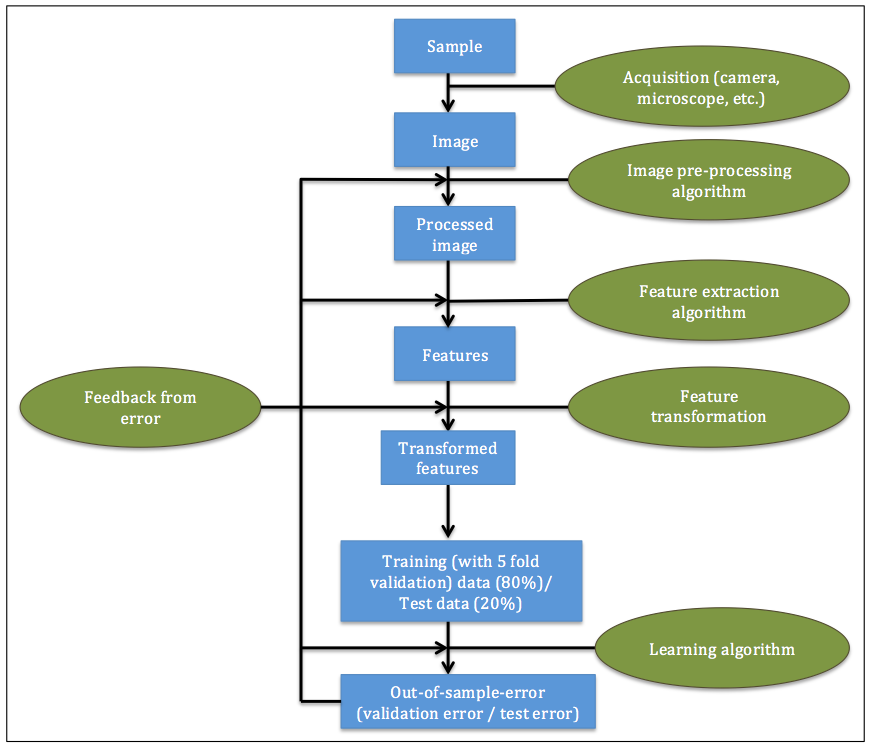
\includegraphics[scale=0.5]{img/EP/flowchart}
    \caption{Representation of an image classification pipeline}
\label{fig:flowchart1}
\end{figure}

the flowchart starts with a sample that is imaged with acquisition technology like a camera or a microscope. The image is then processed using image pre-processing algorithms like normalization and standardization. This may also include image segmentation algorithms. This is followed by feature extraction algorithms that extract useful information from the images. Sometimes, the features extracted are transformed to a different vector space using feature transformation (feature selection or dimensionality reduction) algorithms. The dataset is then divided into training and test datasets in an 80-20 split. Finally, learning algorithms like random forests and logistic regression are used as learning algorithms to build a predictive model for the image classification problem. The performance of the pipeline is evaluated using classification metrics like cross-entropy loss, F1-score, accuracy, precision and recall.  The error in the image classification pipeline maybe measured by such metrics. In this thesis, we base our work on variations of this workflow. Even though the error in image classification pipelines are observed only in terms of the classification error, the source of the error is not just the classification algorithms. The final error is a result of the accumulation of error starting from the beginning of the pipeline right down to the learning algorithms used for classification. Therefore, attempts at improving the performance of image classification pipelines involve the use of  better components in the workflow. This includes using better algorithms and methods for performing data analysis on the image datasets. It may also include improving the quality of the image dataset themselves. Another approach  is to optimize and minimize the error from the pipeline by optimizing the data analytic portion of the pipeline as a whole. This could mean searching the solution space of algorithms to find the best set of algorithms for a particular problem. 
There is also a lack of interpretability of such image classification pipelines, in terms of understanding the source of the errors in the image classification pipeline pertaining to a particular dataset. 
 In this thesis, we present approaches for minimizing the error in image classification with respect to scientific image datasets from different domains. These methods maybe used by domain experts or scientists to train high quality image classification pipelines for similar datasets.  In addition, we also propose methods to quantify the error from all the components of a machine learning pipeline. These methods maybe used by domain experts and data scientists alike to understand and interpret results from image classification pipelines.  

%%% CONTRIBUTIONS
\section{Contributions}
We made the following contributions over the coarse of four projects discussed in the following chapters:
\begin{enumerate}
\item We perform an exhaustive search of data analytic algorithms in the problem of microstructure recognition. The steps included in this work include feature extraction, feature selection and classification algorithms. Each step consists of various algorithms. Two binary image classification tasks are performed in this work. They consist of classification between dendritic and non-dendritic microstructures and between logitudinal and transverse dendrites. We show that this methodology can be used to identify the best configuration of algorithms and hyperparameters in the domain of microstructure recognition.
An exhaustive grid search on the pipeline also shows that pre-trained convolutional neural networks maybe used to represent images of microstructures in the domain of material science

\item We report an automated method for characterization of microvessel morphology by performing data augmentation using parametric 3D models of neuropathological blood vessels. We show that a combination of natural and artificial data perform better in terms of classification metrics.  We propose the development of parametric 3D models of blood vessels and this is used to augment datasets for two classification tasks that involve the classification of morphology of blood vessels. The consist of the classification between singular blood vessels and double blood vessels, and between vessels that consist of lumen and those that don't.

\item We propose a  automated machine learning based score to quantify the quality of an image. This method maybe used to filter a dataset based on the quality of the images. This method can be used by domain experts to perform data analysis on a dataset that only consists of images with a high amount of signal. 

\item We propose an \textit{agnostic} methodology to quantify the contribution of errors from different components of an image classification pipeline. 
We show empirically that performing global random search on the entire pipeline maybe used for efficiently computing the statistics of error contribution from computational steps and algorithms in the image classification pipeline.

\end{enumerate}

%%% OUTLINE
\section{Outline}
The following chapters detail our contributions with respect to optimization and quantification of error in image classification pipelines.
In Chapter \ref{chap:COMMAT}, we describe the problem of microstructure recognition with respect to two classification tasks. 
In Chapter \ref{chap:ISBI}, we propose the parametric 3D model based data augmentation method used in classification of morphologies of blood vessels in neuropathological tissue samples. 
In Chapter \ref{chap:SPIE1}, we present a machine learning based \textit{Quality of Image} score that can automatically quantify whether the image is \textit{good} or \textit{bad}.
In Chapter \ref{chap:EP}, we propose and describe a methodology to quantify the contributions of error from different components of an image classification pipeline. 
In Chapter \ref{chap:conclusions} we present summarized conclusions and discuss relevant future
work. 
%\chapter{AN AUTOMATED APPROACH FOR PARALLEL ADJOINT-BASED
ERROR ESTIMATION AND MESH ADAPTATION FOR STEADY-STATE
PROBLEMS}
\label{chap:automated}

\let\thefootnote\relax\footnotetext{
This chapter has been submitted to:
B.~N. Granzow, A.~A. Oberai, and M.~S. Shephard,
``An automated approach for parallel adjoint-based error
estimation and mesh adaptation,'' submitted for publication.}

%%% INTRODUCTION
\section{Introduction}

To make adjoint-based
error estimation and mesh adaptation more accessible to solid mechanics
practitioners, we seek to fully automate its steps for execution on
parallel machines. Specifically, we seek to
develop software that automates steps 1-6 outlined in Chapter \ref{chap:intro}
based solely on the
inputs of a semilinear form $\R$ and a functional QoI $J$. We endeavor to
develop this software to be applicable to both Galerkin and stabilized
finite element methods.

Recently, Rognes and Logg \cite{rognes2013automated} introduced a fully
automated approach to goal-oriented error estimation and mesh adaptation for
Galerkin finite element methods within the FEniCS \cite{logg2012automated}
finite element framework. In this approach, the adjoint problem is derived
in a discrete manner based on a user-implemented residual $\R$ and a
functional $J$. The adjoint problem is then solved on the same finite element
space as used for the primal problem and enriched to a higher order
polynomial space by solving local patch-wise problems.
Based on the given semilinear form
$\R$, error contributions are then localized to the element-level by solving
local element problems to recover the strong form of the residual operator
over element interiors and element boundaries. The total error in the
functional QoI is then computed as the sum of these error contributions. As a
final step, the mesh is adapted using conforming unstructured mesh
\emph{refinement}.

In this work, we present an approach for automating goal-oriented
analysis that is distinct in several ways. First, we consider adjoint-based
error estimation in the context of both Galerkin and stabilized finite element
methods. Additionally, we propose solving the adjoint problem in a richer
finite element space, obtained via uniform refinement, than the space used for
the primal problem. To localize the error to the mesh entity level,
we utilize a partition of unity based approach proposed by Richter
and Wick \cite{richter2015variational}. This allows us to directly re-use the
implemented semilinear form $\R$ for error localization, eliminating the need
to solve local element problems to recover the strong form residual. We also
take advantage of fully unstructured conforming mesh adaptation, where the
mesh can be \emph{coarsened} as well as refined. As a final distinction, we
highlight the ability of the proposed approach to execute on parallel machines.

In totality, our new approach can be described as follows. First, the primal
problem is solved via Newton's method, where the Jacobian of the semilinear
form $\R$ is obtained via automatic differentiation. The adjoint problem is
derived in a discrete manner in a richer finite element space obtained by a
uniform refinement of the initial mesh. The adjoint operator is derived by an
application of automatic differentiation to the semilinear form $\R$, and the
right-hand side of the adjoint problem is obtained by applying automatic
differentiation to the functional $J$. An approximate error $\eta$ is computed
as a modified discrete adjoint weighted residual evaluated on the fine space.
The error is then localized to mesh vertices using a variational localization
approach by introducing a partition of unity into the weighting slot of the semilinear form
$\R$. An approximate upper bound $\hat{\eta}$ is obtained by summing the
absolute values of localized error contributions. Finally, the mesh is adapted
by specifying a \emph{mesh size field}, which defines the length of mesh
edges over the mesh. We have implemented this approach in a \texttt{C++}
finite element application which we have called Goal \cite{goal_github}.

Underlying this approach is the concept of \emph{template-based generic
programming} (TBGP) \cite{pawlowski2012automating1, pawlowski2012automating2},
which has previously been used to automate the solution of PDEs as well as
embedded advanced analysis features, such as
sensitivity analysis and uncertainty quantification. From a high-level the
TBGP approach consists of a \emph{gather} phase, a \emph{compute} phase,
and a \emph{scatter} phase. The present work extends the TBGP approach to
include the automation of error localization, as required to drive
mesh adaptation.

The remainder of this chapter is outlined as follows.
First adjoint-based error estimation is reviewed for abstract
Galerkin and stabilized variational problems.
Next, a description of the software components utilized in this
work is provided. In particular, each step of the automated
adjoint-based analysis is discussed with respect to its utilized software
components. A review of the concept of TBGP is then provided
and its extension for the purposes of adjoint-based error estimation
is discussed. A detailed description of each step in the
adaptive adjoint-based process is then described. First the
automated solution of the primal problem is discussed. Then
the automated derivation and solution of the adjoint problem
is described. Next, the automation of error localization to
drive mesh adaptation is outlined and mesh adaptation procedures
are discussed. The implementation of several QoIs in the Goal
application is reviewed. Finally, the effectiveness of the
proposed automated approach is demonstrated for several
applications.

%%% A REVIEW OF ADJOINT-BASED ERROR REPRESENTATIONS
\section{A Review of Adjoint-Based Error Representations}

In this section, a brief review of the derivation of adjoint-based
error representations is provided for Galerkin finite element methods as
outlined by Becker and Rannacher \cite{becker2001optimal}, and for
stabilized finite element methods as outlined by Cyr et al. \cite{cyr2014approaches}.
This review is inteded to give context and serve as a road map for the remaining
sections in this chapter.

Let $\S$ and $\V$ be Hilbert spaces, $\R_g : \S \to \V$ and
$\R_{\tau} : \S \to \V$ be semilinear forms that are linear in their first
argument and potentially nonlinear in their second argument. Let
$\S^H \subset \S$ and $\V^H \subset \V$ be classical finite element
function spaces, where $H$ is a mesh-dependent parameter that denotes the
fineness of the discretization. We introduce the following variational
abstract model problem: find $u \in \S$ such that
%
%% aut_abstract_primal
\begin{gather}
\R_g(w; u) = 0 \quad \forall w \in \V.
\label{eq:aut_abstract_primal}
\end{gather}
%
Similarly, we introduce the following abstract \emph{adjoint problem}:
find $z \in \V$ such that
%
%% aut_abstract_adjoint
\begin{gather}
\R_g'[u^H](w, z) = J'[u^H](w) \quad \forall w \in \V,
\label{eq:aut_abstract_adjoint}
\end{gather}
%
where the prime indicates Fr\'{e}chet linearization about the argument in
square brackets, which can equivalently be expressed as the G\^{a}teaux
derivatives
%
% aut_functional_deriv
\begin{gather}
J'[u^H](w) :=
\frac{d}{d \epsilon} J(u^H + \epsilon w) \bigr|_{\epsilon = 0},
\end{gather}
%
and
%
%% aut_resid_deriv
\begin{gather}
\R_g'[u^H](w, z) :=
\frac{d}{d \epsilon} \R(z; u^H + \epsilon w) \bigr|_{\epsilon = 0}.
\end{gather}
%
Here, $u^H \in \S^H$ denotes some finite element approximation to the
true solution $u$. The purpose of the adjoint problem is to relate the
original problem of interest to the functional quantity $J$, and it is this
relationship that allows us to derive adjoint-based error representations.
Further, we note that the adjoint solution $z$ can be interpreted as
the sensitivity of the QoI to perturbations in the primal PDE residual
\cite{fidkowski2011review}.

%%% GALERKIN FINITE ELEMENT METHODS
\subsection{Galerkin Finite Element Methods}

The corresponding Galerkin finite element formulation of the abstract
problem \eqref{eq:aut_abstract_primal} can be stated as: find
$u^H \in \S^H$ such that
%
%% aut_abstract_fem
\begin{gather}
\R_g(w^H; u^H) = 0 \quad \forall w^H \in \V^H.
\label{eq:aut_abstract_fem}
\end{gather}
%
Let $e := u-u^H$ denote the discretization error. We can then derive an
error representation for the functional $J$ in terms of the adjoint solution
$z$ as follows:
%
%% aut_abstract_galerkin_error
\begin{gather}
\begin{aligned}
J(u) - J(u^H) &= J'[u^H](e) + \O(e^2) \\
&= \R_g'[u^H](e, z) + \O(e^2) \\
&= \R_g(z; u) - \R_g(z; u^H) + \O(e^2) \\
&= - \R_g(z; u^H) + \O(e^2) \\
&= - \R_g(z - z^H; u^H) + \O(e^2).
\end{aligned}
\label{eq:aut_abstract_galerkin_error}
\end{gather}
%
Here, the first equality is due to the linearization \cite{becker2001optimal}
of the functional $J$, the second equality is due to the introduced adjoint
problem \eqref{eq:aut_abstract_adjoint}, the third equality is due to the
linearization \cite{becker2001optimal} of the residual $\R_g$, the fourth
equality holds due to the definition of the abstract primal problem
\eqref{eq:aut_abstract_primal}, and the fifth equality is due to Galerkin
orthogonality, where $z^H$ denotes the interpolant of $z$ onto the space
$\V^H$. In reference to the notation introduced, the
total residual semilinear form $\R$ is given as $\R = \R_g$.

%%% STABILIZED FINITE ELEMENT METHODS
\subsection{Stabilized Finite Element Methods}

A corresponding stabilized finite element method of the abstract problem
\eqref{eq:aut_abstract_primal} can be expressed as: find $u^H \in \S^H$ such
that
%
%% aut_abstract_stabilized_fem
\begin{gather}
\R_g(w^H; u^H) + \R_{\tau}(w^H; u^H) = 0 \quad \forall w^H \in \V^H.
\label{eq:aut_abstract_stabilized_fem}
\end{gather}
%
Here $\R_{\tau}$ denotes a consistent \emph{stabilization residual} that adds
stability to the numerical scheme. We say that the
stabilization is \emph{consistent} if $\R_{\tau}(w^H ; u) \to 0$ as
$H \to 0$.

Again, we let $e := u - u^H$ denote the discretization error, and derive
an error representation for the functional $J$ as follows
%
%% aut_abstract_stabilized_error
\begin{gather}
\begin{aligned}
J(u) - J(u^H) &= J'[u^H](e) + \O(e^2) \\
&= \R_g'[u^H](e, z) + \O(e^2) \\
&= \R_g(z; u) - \R_g(z; u^H) + \O(e^2) \\
&= - \R_g(z; u^H) + \O(e^2) \\
&= - \R_g(z - z^H; u^H) + \R_{\tau}(z^H; u^H) + \O(e^2).
\end{aligned}
\label{eq:aut_abstract_stabilized_error}
\end{gather}
%
Here, the first four equalities are obtained exactly as in the corresponding
Galerkin finite element method. However, when we subtract the interpolant
$z^H$ of the adjoint solution $z$ in the fifth equality, an additional term
remains because the numerical scheme \eqref{eq:aut_abstract_stabilized_fem}
lacks Galerkin orthogonality. In reference to the notation
introduced, the total semilinear form $\R$ is given as
$\R = \R_g + \R_{\tau}$.

%%% SOFTWARE COMPONENTS
\section{Software Components}

An adaptive adjoint-based simulation
requires the implementation and coordination of a number of
non trivial components. Namely, the solution of a primal problem,
the construction and solution of an auxiliary adjoint problem, an enrichment
of the adjoint solution, the estimation and localization of the error,
and mesh adaptation are all required steps in the adjoint-based
adaptive process.

To implement each of these components for effective execution on parallel
machines, we make use of two state of the art software suites. The first
is PUMI \cite{ibanez2016pumi}, which contains tools to
support unstructured mesh services on massively parallel machines. In
particular, PUMI provides all of the necessary machinery to store, query,
adapt, and dynamically load balance parallel unstructured meshes via
a collection of modern \texttt{C} and \texttt{C++} libraries. The second
is Trilinos \cite{heroux2005overview, heroux2012new}, which provides a
large variety of \texttt{C++} packages to support multiphysics
simulations on parallel machines. In particular, Trilinos provides
the ability to store and solve sparse parallel linear systems, as
well as tools to perform automatic differentiation.

Using these two software suites as building blocks, we have written a new
\texttt{C++} application for adjoint-based error estimation and mesh
adaptation with an emphasis on nonlinear solid mechanics. We have called this
application Goal \cite{goal_github}. Below, we describe
how these software components are
utilized for each portion of the adaptive adjoint-based process,
where the analysis is automated based only on the inputs of a semilinear
form $\R$ and a functional QoI $J$.

%%% THE PRIMAL PROBLEM
\subsection{The Primal Problem}

Based on an implemented weighted residual operator $\R$, the Goal
application computes element-level residual vectors and element-level
Jacobian matrices. The element-level Jacobian matrices are computed via
automatic differentiation using the Trilinos library Sacado. Sacado
provides efficient automatic differentiation using a \texttt{C++}
meta-programming technique called expression templates
\cite{phipps2012efficient}.

After the computation of a single element's residual vector and Jacobian
matrix, the Goal application performs a finite element assembly step to
sum contributions to the global residual vector and global Jacobian matrix.
To store and modify the global linear algebra objects, we utilize the Tpetra
library provided by Trilinos. In particular, the Jacobian matrix is stored
as a sparse compressed row storage matrix in parallel.

The primal problem is solved via Newton's method, which requires iterative
evaluations of the global residual vector and Jacobian matrix. For each
Newton iteration, a global linear system must be solved. We solve
this linear system iteratively in parallel using either a CG or GMRES solver provided
the Trilinos library Belos \cite{bavier2012amesos2}. Additionally, we
perform algebraic multigrid preconditioning using the Trilinos library
MueLu \cite{MueLu}.

Once the primal problem has been solved, we utilize the PUMI library APF
to store the finite element solution information at nodes and if necessary
secondary solution information at integration points. Additionally, the APF
library is used to provide shape function information and to query stored
solution information during residual and Jacobian evaluations. Throughout
the entire solution process, the PUMI mesh data structure is utilized to
query mesh specific information.

%%% THE ADJOINT PROBLEM
\subsection{The Adjoint Problem}

To solve the adjoint problem in a richer finite element space than the one
used for the primal problem, we make use of the underlying PUMI mesh data
structure \cite{ibanez2017modifiable} and the PUMI MeshAdapt software to
create and store a uniformly refined nested mesh with parent-child relations
back to the original mesh. This relational information is implemented in the
Goal application, as it falls outside of the normal intended use case of the
MeshAdapt software, which concerns itself with fully unstructured conforming
mesh adaptation via edge splits, swaps, and collapses. However,
the flexibility of the PUMI software allows us to
additionally construct data structures similar to those used in traditional
adaptive mesh refinement (AMR) with little implementation effort. Using
the APF library and the parent-child relational information, we are able
to interrogate stored solution fields on both the parent and nested meshes,
which is required during the assembly of the adjoint problem.

On this finer mesh, element-level Jacobian matrices are computed using the
Sacado library, based on the Goal implementation of the operator $\R$.
Additionally, element-level derivatives of the functional quantity of
interest $J$ are computed with respect to degrees of freedom of the problem,
resulting in an element-level functional derivative vector.

After the computation of a single element's Jacobian matrix and functional
derivative vector, the Goal application performs a finite element assembly
step to sum contributions to the global discrete adjoint matrix and the
global functional derivative vector. Like the primal problem, these global
parallel linear objects are stored using the Tpetra library. The global
discrete adjoint operator and functional derivative vector fully define the
linearized adjoint problem, which we again precondition with algebraic
multigrid techniques using the MueLu library and solve using either CG
or GMRES iterations using the Belos library. The fine-space adjoint solution
is then attached to the mesh using the APF library.

%%% ERROR ESTIMATION AND LOCALIZATION
\subsection{Error Estimation and Localization}

The error estimation and localization routines are implemented entirely in
the Goal application. The error is localized by an evaluation of the
stabilized weighted residual operator $\R$, where the weight is chosen to be
the adjoint solution multiplied by a partition of unity. Based on these
element-level residual vectors, Goal performs finite element assembly
of the global residual vector, which is stored as a Tpetra vector. This
vector represents an adjoint-weighted residual error estimate at each mesh
vertex for each PDE equation in the fine mesh. The error is attached to the
vertices of the fine mesh using the APF library.

%%% MESH ADAPTATION
\subsection{Mesh Adaptation}

Once the error is stored on the vertices of the fine mesh, we interpolate
it to element centers of the coarse mesh. The fine mesh data structures are
then destroyed and the Goal application computes a mesh size field that
seeks to equidistribute the error for an output mesh with $N$ elements. This
mesh size field is given as the input to the PUMI MeshAdapt software, which
adapts the mesh with a sequence of edge splits, swaps, and collapses
\cite{li20053d, alauzet2006parallel} to satisfy the given mesh size field.
As a final step, we utilize the PUMI library ParMA
\cite{smith2015parma, diamond2017dynamic}
to perform diffusive
load balancing to ensure parallel partitioning quality.

%%% IN-MEMORY INTEGRATION
\subsection{In-Memory Integration of Components}

The coupling of both the analysis and
software components described above is done \emph{in-memory}
\cite{smith2016memory}. That is, there is no file-based communication of
data from one analysis component to the next in the automated process.
This in-memory coupling is a key ingredient for parallel analysis,
where filesystem bandwidth is a critical bottleneck.

%%% TEMPLATE-BASED GENERIC PROGRAMMING
\section{Template-Based Generic Programming}
\label{sec:tbgp}

In this section, we provide a review of the concept of
\emph{template-based generic programming} for the evaluation and solution of
PDEs \cite{pawlowski2012automating1,pawlowski2012automating2} and how it
has been extended in the Goal application to automate the process of
adjoint-based error estimation and mesh adaptation. 
For PDE applications, TBGP is broken into three major components,
a \emph{seed} or \emph{gather} phase, a \emph{compute} phase, and
a \emph{scatter} phase. The seed and scatter operations must be
programmed specifically for each evaluation purpose. In contrast, the
compute phase, where the PDE and QoI expressions are implemented,
are written in a totally generic manner. Figure \ref{fig:mech_tbgp}
pictorially represents this design philosophy.

\begin{figure}[ht!]
\centering
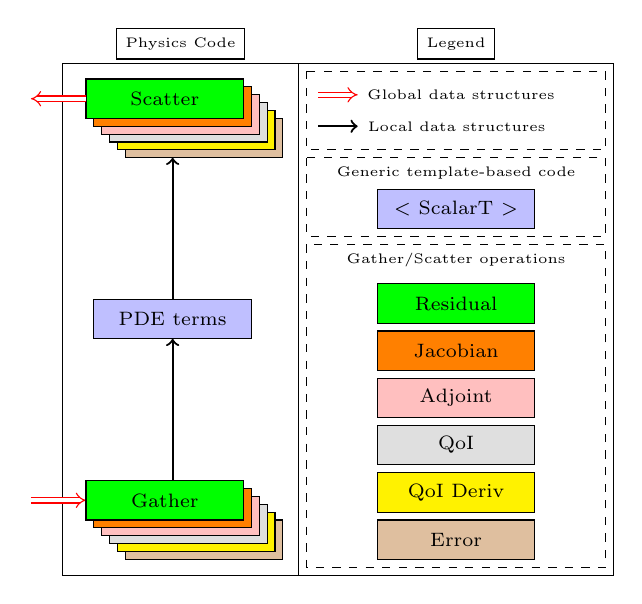
\begin{tikzpicture}

% physic code
\node[draw] at (1.5,6.25) {\tiny Physics Code};

% legend
\node[draw] at (5, 6.25) {\tiny Legend};

% bounding boxes
\draw (0,-0.5) rectangle +(3, 6.5);
\draw (3,-0.5) rectangle +(4, 6.5);

% global data transfer -> gather
\draw[red,-implies,double equal sign distance] (-0.4,0.45) -- (0.3,0.45);

% gather template operations
\draw[fill=brown!50] (0.8, -0.3) rectangle+(2,0.5);
\draw[fill=yellow] (0.7, -0.2) rectangle+(2,0.5);
\draw[fill=gray!25] (0.6, -0.1) rectangle+(2,0.5);
\draw[fill=pink] (0.5, 0.0) rectangle+(2,0.5);
\draw[fill=orange] (0.4, 0.1) rectangle+(2,0.5);
\draw[fill=green] (0.3, 0.2) rectangle +(2,0.5)
node[pos=0.5] {\scriptsize Gather};

% local data transfer gather -> pde
\draw[black,thick,->] (1.4,.7) -- (1.4,2.5);

% generic template pde evaluation
\draw[fill=blue!25] (0.4,2.5) rectangle +(2,0.5)
node[pos=0.5] {\scriptsize PDE terms};

% local data transfer pde -> scatter
\draw[black,thick,->] (1.4,3.0) -- (1.4,4.8);

% scatter template operations
\draw[fill=brown!50] (0.8, 5.3) rectangle+(2,-0.5);
\draw[fill=yellow] (0.7, 5.4) rectangle+(2,-0.5);
\draw[fill=gray!25] (0.6, 5.5) rectangle+(2,-0.5);
\draw[fill=pink] (0.5, 5.6) rectangle+(2,-0.5);
\draw[fill=orange] (0.4, 5.7) rectangle+(2,-0.5);
\draw[fill=green] (0.3, 5.8) rectangle+(2,-0.5)
node[pos=0.5] {\scriptsize Scatter};

% global data transfer <- scatter
\draw[red,implies-,double equal sign distance] (-0.4,5.55) -- (0.3,5.55);

% data transfer
\draw[dashed] (3.1,5.9) rectangle +(3.8,-1);
\draw[red,-implies,double equal sign distance] (3.25,5.6) -- (3.75,5.6)
node[black,anchor=west] {\tiny Global data structures};
\draw[black,thick,->] (3.25, 5.2) -- (3.75, 5.2)
node[black,anchor=west] {\tiny Local data structures};

% generic data evaluation type
\draw[dashed] (3.1, 4.8) rectangle +(3.8,-1);
\node[black] at (5,4.6) {\tiny Generic template-based code};
\draw[fill=blue!25] (4,4.4) rectangle +(2,-0.5)
node[pos=0.5] {\scriptsize $<$ ScalarT $>$};

% template specializations
\draw[dashed] (3.1, 3.7) rectangle +(3.8,-4.1);
\node[black] at (5,3.5) {\tiny Gather/Scatter operations};
\draw[fill=green] (4,3.2) rectangle +(2,-0.5)
node[pos=0.5] {\scriptsize Residual};
\draw[fill=orange] (4,2.6) rectangle +(2,-0.5)
node[pos=0.5] {\scriptsize Jacobian};
\draw[fill=pink] (4,2.0) rectangle +(2,-0.5)
node[pos=0.5] {\scriptsize Adjoint};
\draw[fill=gray!25] (4,1.4) rectangle +(2,-0.5)
node[pos=0.5] {\scriptsize QoI};
\draw[fill=yellow] (4,0.8) rectangle +(2,-0.5)
node[pos=0.5] {\scriptsize QoI Deriv};
\draw[fill=brown!50] (4,0.2) rectangle +(2,-0.5)
node[pos=0.5] {\scriptsize Error};
\end{tikzpicture}

\caption{A schematic for the generic programming model of PDEs.}
\label{fig:mech_tbgp}
\end{figure}

We invoke this approach at the element-level, meaning for each element
we perform the process: Gather $\rightarrow$ Compute $\rightarrow$
Scatter. By doing so, we reduce memory overhead and eliminate complications
introduced by parallel computation \cite{pawlowski2012automating2}.
Underlying the TBGP approach is the use of forward automatic differentiation
(FAD) \cite{griewank2008evaluating}, which is discussed in further detail
in Appendix \ref{chap:fad}. The Goal application utilizes the
Trilinos library Sacado \cite{phipps2012efficient} to perform
automatic differentiation.

\begin{table}[ht!]
\tabulinesep=1.2mm
\centering
\begin{tabu}{| l |  l | c | c |} \hline
Evaluation Type & Scalar Type & Input & Output \\ \hline \hline
Residual & \texttt{double} & $\bs{u}^H, \bs{s}^H$ & $\bs{R}^H$ \\ \hline
Jacobian & \texttt{Sacado::FAD} & $\bs{u}^H, \bs{s}^H$ & $\frac{\partial \bs{R}^H}{\partial \bs{u}^H}$ \\ \hline
Adjoint & \texttt{Sacado::FAD} & $\bs{u}^h_H, \bs{s}^h_H$ & $\left[ \frac{\partial \bs{R}^h}{\partial \bs{u}^h} \bigr|_{\bs{u}^h_H} \right]^T$ \\ \hline
QoI & \texttt{double} & $\bs{u}^H, \bs{s}^H$ & $J^H$ \\ \hline
QoI Deriv & \texttt{Sacado::FAD} & $\bs{u}^h_H, \bs{s}^h_H$ & $ \left[ \frac{ \partial J^h} { \partial \bs{u}^h} \bigr|_{\bs{u}^h_H} \right]^T $ \\ \hline
Error & \texttt{double} & $\bs{u}^h_H, \bs{s}^h_H, \bs{z}^h$ & $\bs{R}^h$ \\ \hline
\end{tabu}
\caption{A list of TBGP evaluation operations used in the Goal application.
In this table $\bs{u}^H$ is the primal solution vector, $\bs{u}^h_H$ is the
prolongation of the solution vector to a richer space, $\bs{s}^H$ is a
(potentially empty) vector of history-dependent mechanics state variables,
$\bs{s}^h_H$ is the prolongation of the state to a richer space,
$\bs{z}^h$ is the adjoint solution vector,
$\bs{R}^H$ is the residual vector evaluated on the coarse space,
$\bs{R}^h$ is the residual vector evaluated on the fine space, and
$J^H$ is the scalar QoI.}
\label{tab:software_evaluations}
\end{table}

The purpose of the gather/seed operation is to collect information
from global storage containers and `gather' it to local element-level
data structures. Further, any FAD derivative information is \emph{seeded}
during this operation, if necessary. For each evaluation type, the
gather/seed operation initializes an array that physically represent the
degrees of freedom associated with the current element, and
initializes FAD variables' derivative arrays to physically represent
derivatives with respect to the degrees of freedom associated with
the current element, when necessary. This degree of freedom array is
templated on a scalar type \texttt{ScalarT}. For the Residual, QoI,
and Error evaluation types, this scalar type corresponds to a
\texttt{C++} double. For the remaining evaluation types, this
scalar type corresponds to a \texttt{Sacado::FAD} forward automatic
differentiation variable type.

The compute phase computes local contributions to the equations or
expressions of interest at the element level in terms of the degrees
of freedom, as collected by the gather operation. The code for the
compute phase is written in an entirely generic fashion, and is templated
on a scalar type \texttt{ScalarT}. Templating the code used for the
compute phase, along with appropriately chosen gather and scatter
operations, allows the same code to be re-used for the distinct
evaluation purposes listed in Table \ref{tab:software_evaluations}.

The scatter phase takes the local element-level data
evaluated in the compute phase and `scatters' it to the appropriate
global data structure, as determined by the current evaluation operation.
For instance, for the residual evaluation operation, local element-level
residuals are evaluated in the compute phase and then summed into
appropriate locations in the global residual vector during the scatter
phase. Similarly, for the Jacobian evaluation operations, local element-level
Jacobians are evaluated in the compute phase and the scatter opeation
sums these local contributions to appropriate locations in the global
Jacobian matrix.

\begin{lstlisting}[
float,
style=mystyle,
caption=The abstract Goal integrator class interface,
label=lst:software_integrator]
class Integrator {
  public:
    Integrator();
    virtual ~Integrator();
    std::string const& get_name() { return name; }
    virtual void set_time(double, double) {}
    virtual void pre_process(SolInfo*) {}
    virtual void set_elem_set(int) {}
    virtual void gather(apf::MeshElement*) {}
    virtual void in_elem(apf::MeshElement*) {}
    virtual void at_point(apf::Vector3 const&, double, double) {}
    virtual void out_elem() {}
    virtual void scatter(SolInfo*) {}
    virtual void post_process(SolInfo*) {}
  protected:
    std::string name;
\end{lstlisting}

In the Goal application, we have considered six specific gather/scatter
evaluation operations corresponding to the evaluation of the global
residual vector, evaluation of the global Jacobian matrix, evaluation
of the adjoint of the global Jacobian matrix, evaluation of the
functional QoI, evaluation of the derivative of the functional QoI,
and evaluation of localized adjoint-weighted residual error estimates.
Table \ref{tab:software_evaluations} lists the inputs and outputs for
these specific evaluation operations.

To realize these specific gather/scatter operations, we have implemented
an abstract degree of freedom class and an abstract quantity of interest
class that are both templated on a scalar type \texttt{ScalarT}. This
scalar type is explicitly instantiated to either be a \texttt{C++} double
or a \texttt{Sacado::FAD} forward automatic differentiation variable type.
Both the degree of freedom and QoI classes are equipped with \texttt{gather}
and \texttt{scatter} methods, whose behavior changes based on an input
parameter given to the class constructor. For the degree of freedom
class, this parameter selects gather/scatter operations for either the
residual, Jacobian, adjoint Jacobian, or adjoint-weighted residual error
evaluations. Similarly, for the QoI class, this input parameter selects
gather/scatter operations for either the evaluation of the QoI
or the derivative of the QoI with respect to the problem degrees of freedom.

Previously, TBGP has been utilized in the multiphysics code
Albany \cite{salinger2013albany, tezaur2015albany} with the capability
to perform the Residual, Jacobian, Adjoint, QoI, and QoI derivative
evaluation operations shown in Table \ref{tab:software_evaluations}.
To extend the abilities of TBGP to include adjoint-based error estimation,
the Goal application implements the ability to perform the Adjoint and
QoI derivative evaluations in a richer finite element space, as
discussed in Section \ref{sec:aut_adjoint}, a feature not previously
available in existing TBGP codes. Further, the Goal application implements a
novel evaluation type for the localization of the error, referred to as the
Error evaluation type in Table \ref{tab:software_evaluations}. For this purpose,
we have implemented an abstract weighting function class whose
behavior changes based on the chosen evaluation type. This class
evaluates the appropriate finite element weighting function values
and gradients based on linear Lagrange basis functions for the
Residual, Jacobian and Adjoint evaluation types. However, for the
Error evaluation type, the behavior of the weighting function
class is modified such that it evaluates the value and gradient
of the adjoint solution $z^h$ multiplied by a partition of unity. This abstraction of the
weighting function class
allows us to re-use the PDE implementation of the semilinear form
$\R$ to assemble a residual vector $\bs{R}^h$ that represents an
adjoint-weighted residual error estimate at each mesh vertex for each PDE
equation in the richer finite element space, which is then used
to drive mesh adaptation.

Listing \ref{lst:software_integrator} demonstrates the abstract
integrator interface that has been implemented in the Goal
application. The abstract degree of freedom, QoI, and
weighting function classes inherit from this base class.
For each of these classes, the \texttt{gather} and \texttt{scatter}
methods are implemented specifically for each appropriate
evaluation type. The PDE equations in the Goal application are
written as a combination of \texttt{Goal::Integrator}s.
Given  an ordered array of integrators, the Goal application
performs finite element assembly for every evaluation type
in a generic manner, as outlined by Algorithm \ref{alg:software_assembly}.

\begin{algorithm}
\caption{Assembly algorithm used in the Goal application}
\begin{algorithmic}
\State Given a mesh $M$ and an ordered array of integrators $I$:
\State Call \texttt{pre\_process} for each integrator $i$ in $I$.
\For{ each element set $es$ in mesh $M$ }
\State Call \texttt{set\_elem\_set} for each integrator $i$ in $I$.
\For{ each element $e$ in element set $es$ }
\State Call \texttt{gather} for each integrator $i$ in $I$.
\State Call \texttt{in\_elem} for each integrator $i$ in $I$.
\For{ each integration point $ip$ in element $e$ }
\State Call \texttt{at\_point} for each integrator $i$ in $I$.
\EndFor
\State Call \texttt{out\_elem} for each integrator $i$ in $I$.
\State Call \texttt{scatter} for each integrator $i$ in $I$.
\EndFor
\EndFor
\State Call \texttt{post\_process} for each integrator $i$ in $I$.
\end{algorithmic}
\label{alg:software_assembly}
\end{algorithm}

%%% THE PRIMAL PROBLEM
\section{The Primal Problem}

%%% GALERKIN FINITE ELEMENT METHODS
\subsection{Galerkin Finite Element Methods}

We recall the definition of the abstract Galerkin finite element model
problem, given by equation \eqref{eq:aut_abstract_fem}. In this context,
the weighted residual form $\R_g$ is implemented in the Goal application.
As an example, Listing \ref{lst:presidual} demonstrates the implementation
of the Poisson residual $\R_g(w; u) := (\nabla w, \nabla u) - (w,f)$ in
the Goal application.

\begin{lstlisting}[
float,
style=mystyle,
caption=Poisson residual,
label=lst:presidual]
template <typename ScalarT>
void Residual<ScalarT>::at_point(
    apf::Vector3 const& p, double ipw, double dv) {
  apf::Vector3 x(0,0,0);
  apf::mapLocalToGlobal(elem, p, x);
  double fval = eval(f, x[0], x[1], x[2], 0.0);
  for (int n = 0; n < u->get_num_nodes(); ++n)
  for (int i = 0; i < num_dims; ++i)
    u->resid(n) += u->grad(i) * w->grad(n, i) * ipw * dv;
  for (int n = 0; n < u->get_num_nodes(); ++n)
    u->resid(n) -= fval * w->val(n) * ipw * dv;
}
\end{lstlisting}

%%% STABILIZED FINITE ELEMENT METHODS
\subsection{Stabilized Finite Element Methods}

We recall the definition of the abstract stabilized finite element model
problem, given by equation \eqref{eq:aut_abstract_stabilized_fem}. In this
context, both the weighted residual statement $\R_g$ and the stabilized
weighted residual form $\R_{\tau}$ are implemented in the Goal application.
As an example, Listing \ref{lst:stabresidual} demonstrates the implementation
of the pressure stabilization \cite{ramesh2005stabilized} residual
$\R_{\tau}(w; u)$ term used in the Goal application for finite deformation
solid mechanics.

\begin{lstlisting}[
float,
style=mystyle,
caption=Pressure stabilization residual for mechanics,
label=lst:stabresidual]
template <typename ScalarT>
void Stabilization<ScalarT>::at_point(
    apf::Vector3 const&, double ipw, double dv) {
  double h = get_size(mesh, elem);
  double tau = 0.5*c0*h*h/mu;
  auto J = k->get_det_def_grad();
  auto F = k->get_def_grad();
  auto Cinv = inverse(transpose(F)*F);
  for (int n = 0; n < p->get_num_nodes(); ++n)
  for (int i = 0; i < num_dims; ++i)
  for (int j = 0; j < num_dims; ++j)
    p->resid(n) += tau * J * Cinv(i, j) *
      p->grad(i) * w->grad(n, j) * ipw * dv;
}
\end{lstlisting}

%%% AUTOMATED SOLUTION BASED ON RESIDUAL IMPLEMENTATION
\subsection{Automated Solution Based on Residual Implementation}

For each element, we compute element level
Jacobian matrices by applying automatic
differentiation \cite{griewank2008evaluating} to element-level contributions
to the residual vector. For example, Listing \ref{lst:presidual} demonstrates
how contributions to the element-level Poisson's equation residual
$\R(w; u) = (\nabla w, \nabla u) - (w, f)$ are implemented. The element level
Jacobian matrices are then assembled into the global system Jacobian operator
$\bs{\J}^H \in \mathbb{R}^{N \times N}$, given by
%
%% aut_jacobian
\begin{gather}
\bs{\J}^H = \frac{\partial \bs{R}^H (\bs{u}^H) }{\partial \bs{u}^H}
\end{gather}

Listings \ref{lst:presidual} and \ref{lst:stabresidual} both demonstrate how
element-level contributions to the semilinear forms $\R_g$ and $\R_{\tau}$,
respectively, are computed in the Goal application. Notice that this code
is templated on a scalar type \texttt{ScalarT}. When the scalar type is
chosen as a \texttt{C++} \texttt{double}, element-level contributions to
the residual vector $\bs{R}^H$ are computed. When the scalar type is chosen
as a Sacado forward automatic differentiation variable, element-level
contributions to the Jacobian matrix $\bs{\J}^H$ are computed. This
illustrates a key concept of template-based generic programming, in that
the governing equations need only be implemented once to compute a variety
of additional information.

With the ability to fully assemble the Jacobian matrix $\bs{\J}^H$ and the
residual vector $\bs{R}^H$, we solve the governing equations with Newton's
method, where we iterate over the steps
%
%% aut_netwon
\begin{gather}
\begin{aligned}
\bs{\J}^H (\bs{u}^H_k) \, \delta \bs{u}^H_k &=
- \bs{R}^H( \bs{u}^H_k) \\
\bs{u}^H_{k+1} &= \bs{u}^H_k + \delta \bs{u}^H_k,
\end{aligned}
\end{gather}
%
unitl the convergence criterion $\| \bs{R}^H(\bs{u}^H) \|_2 < \epsilon$ is met
for a user-specified tolerance $\epsilon$. Here $\bs{u}^H_k$ denotes the
solution vector at the $k^{th}$ iteration obtained by solving the Newton
linear system. For linear variational problems, we simply restrict ourselves
to a single Newton linear solve, which reduces exactly to classical FEM
assembly for linear problems.

%%% THE ADJOINT PROBLEM
\section{The Adjoint Problem}
\label{sec:aut_adjoint}

%%% A RICHER SPACE VIA UNIFORM REFINEMENT
\subsection{A Richer Space via Uniform Refinement}

The adjoint solution must be represented in a richer
space than the one used for the primal problem to obtain meaningful error
estimates. There are several strategies that are commonly used to obtain
such a representation. First, the adjoint problem can be solved in the same
finite element space as the primal problem and then be enriched to a higher
order polynomial space \cite{becker2001optimal} or a nested mesh
\cite{nemec2007adjoint} by some local patch-wise operation, or variational
multiscale enrichment \cite{granzow2017output} can be used in the context
of stabilized finite elements. Alternatively, the adjoint problem can be solved in a
higher order polynomial space \cite{fidkowski2011output}, which we will refer
to as $p$-enrichment. As a final option, the adjoint problem can be solved on a
uniformly refined mesh \cite{burstedde2009parallel}, which we will refer to
as $h$-enrichment.

In this work, we choose the $h$-enrichment approach for several reasons.
First, we would like the adjoint solution to be as accurate as possible
for error estimation purposes, so we choose to solve the adjoint problem in
a globally richer finite element space. Additionally, for stabilized finite
element methods, the use of $p$-enrichment would in general necessitate the
use of higher order stabilization terms that vanish for lower-order finite
element methods with simplical elements. These higher order terms are
typically more difficult to implement than their lower order counterparts.
Further, we remark that higher-order stabilized finite element methods are
rarely used in practice, as stable higher-order mixed methods can usually
be derived with fewer overall degrees of freedom \cite{taylor1973numerical}.
Finally, we note that the unstructured mesh adaptation capabilities of the
PUMI software make the $h$-enrichment approach readily available.

We have denoted the trial and test spaces used for the primal problem
as $\S^H$ and $\V^H$, respectively. We denote the trial and test spaces on
the uniformly nested mesh as $\S^h$ and $\V^h$, respectively, where $h < H$
is representative of a finer mesh size. Figure \ref{fig:aut_glial_nested}
illustrates the discretization for the coarse and fine trial and test spaces
defined for a three dimensional geometry with a complex void inclusion.

\begin{figure}[ht!]
\centering
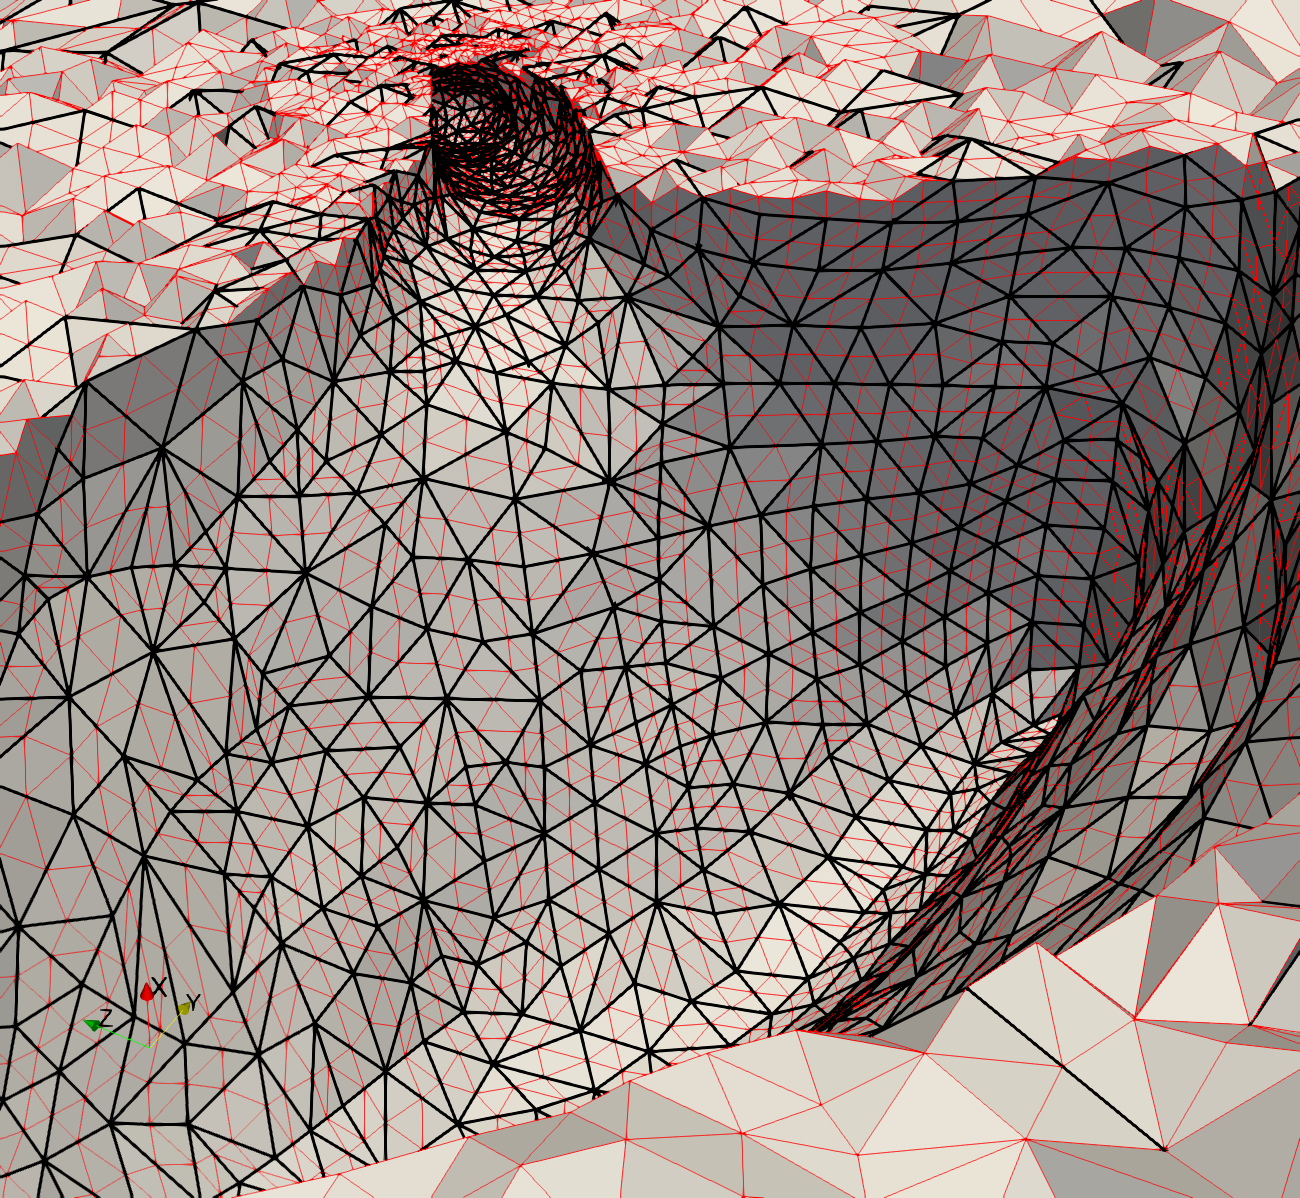
\includegraphics[width=0.5\textwidth]{img/aut_glial_nested}
\caption{Example of a nested mesh (red edges) obtained via a uniform
refinement of a base mesh (black edges) in three dimensions.}
\label{fig:aut_glial_nested}
\end{figure}

%%% DISCRETE ADJOINT APPROXIMATION
\subsection{Discrete Adjoint Approximation}

Let $\bs{R}^h : \mathbb{R}^n \to \mathbb{R}^n$ denote the residual form of
the system of nonlinear algebraic equations arising either from the Galerkin
\eqref{eq:aut_abstract_fem} or stabilized
\eqref{eq:aut_abstract_stabilized_fem}
model problem posed on the uniformly nested mesh. Let $\bs{u}^h_H :=
I^h_H \bs{u}^H$ denote the prolongation of the primal finite element solution
onto the richer space $\S^h$ via interpolation,
Let $J^h : \mathbb{R}^n \to
\mathbb{R}$ denote the discretization of the functional QoI on the
uniformly nested fine space. We approximate the adjoint problem
\eqref{eq:aut_abstract_adjoint} in a discrete manner
\cite{fidkowski2011review, venditti2000adjoint, venditti2002adjoint,
venditti2003adjoint}, by solving
%
%%
\begin{gather}
\left[ \frac{\partial \bs{R}^h}{\partial \bs{u}^h} \biggr|_{u^h_H}
\right]^T \bs{z}^h = \left[ \frac{\partial J^h}{\partial \bs{u}^h}
\biggr|_{u^h_H} \right]^T.
\label{eq:aut_discrete_adjoint}
\end{gather}
%
This allows us to automate the process of solving the adjoint problem, as
discussed below. Here $\bs{z}^h \in \mathbb{R}^n$ denotes the adjoint
solution vector on the nested discretization.

%%% AUTOMATED SOLUTION BASED ON RESIDUAL FORMULATION
\subsection{Automated Solution Based on Residual Formulation}

The construction of the Jacobian transpose matrix $\left[ \partial \bs{R}^h
/ \partial \bs{u}^h \right]^T$ is performed in the same automated manner as
the Jacobian for the primal problem. That is, for each element, we compute
consistent element tangent stiffness matrices via automatic differentiation
of element-level contributions to the residual vector. However, during the
\emph{scatter} phase of the template-based generic programming process,
we transpose the element-level tangent matrices and
sum them into global Jacobian adjoint matrix. The computation of the Jacobian
adjoint is done using the same templated code that is used to compute
the primal residual vector and the Jacobian matrix, as illustrated by
listings \ref{lst:presidual} and \ref{lst:stabresidual}.

Similarly, the construction of the functional derivative vector
$\left[ \partial J^h / \partial \bs{u}^h \right]^T$ is done by evaluating
derivatives of element-level contributions to the functional via automatic
differentiation. This results in element-level derivative vectors that are
then assembled into the global functional derivative vector. Listings
\ref{lst:aut_avg_u_qoi} and \ref{lst:aut_avg_vm_qoi} illustrate the
implementation of two quantities of interest in the Goal application. Once
the Jacobian transpose matrix and functional derivative vector have been
assembled, we solve the adjoint problem \eqref{eq:aut_discrete_adjoint} using
a sparse iterative solver in parallel.

%%% ERROR ESTIMATION
\section{Error Estimation}

%%% TWO LEVEL ERROR ESTIMATES
\subsection{Two-Level Error Estimates}

Following Venditti and Darmofal
\cite{venditti2000adjoint, venditti2002adjoint, venditti2003adjoint},
we review adjoint-based error estimation using two discretization levels.
The discrete residual form of the governing equations for a Galerkin
\eqref{eq:aut_abstract_fem} finite element method or a stabilized finite
element method \eqref{eq:aut_abstract_stabilized_fem} posed on the fine
space can be expressed as
%
%% aut_fine_resid
\begin{gather}
\bs{R}^h(\bs{u}^h) = \bs{0}.
\label{eq:aut_fine_resid}
\end{gather}
%

Taking Taylor expansions of the discrete residual $\bs{R}^h$ evaluated on the
fine space and the discrete functional $J^h$ evaluated on the fine space
about the point $\bs{u}^h_H$ yields
%
%% aut_residual_taylor
\begin{gather}
\bs{R}^h(\bs{u}^h) = \bs{R}^h(\bs{u}^h_H) +
\left[ 
\frac{ \partial \bs{R}^h }{ \partial \bs{u}^h} \biggr|_{\bs{u}^h_H}
\right]
(\bs{u}^h - \bs{u}^h_H) + \dots
\label{eq:aut_residual_taylor}
\end{gather}
%
and
%
%
%% aut_functional_taylor
\begin{gather}
J^h(\bs{u}^h) = J^h(\bs{u}^h_H) +
\left[
\frac{ \partial J^h } { \partial \bs{u}^h} \biggr|_{\bs{u}^h_H}
\right]
(\bs{u}^h - \bs{u}^h_H) + \dots
\label{eq:aut_functional_taylor}
\end{gather}
%
respectively.

Using equation \eqref{eq:aut_fine_resid}, the discretization error
between the two spaces can be approximated to first order as
%
%% aut_disc_error_approx
\begin{gather}
(\bs{u}^h - \bs{u}^h_H) \approx
- \left[
\frac{ \partial \bs{R}^h } { \partial \bs{u}^h } \biggr|_{\bs{u}^h_H}
\right]^{-1}
\bs{R}^h (\bs{u}^h_H ),
\label{eq:aut_disc_error_approx}
\end{gather}
%
which can then be substituted into the functional Taylor expansion
\eqref{eq:aut_functional_taylor} to obtain the so-called
\emph{adjoint weighted residual}
%
%% 
\begin{gather}
J^h(\bs{u}^h) - J^h(\bs{u}^h_H) \approx  - \bs{z}^h \cdot \bs{R}^h(\bs{u}^h_H)
\label{eq:aut_adjoint_weighted_residual}
\end{gather}
%
where $\bs{z}^h$ is the solution to the adjoint problem
\eqref{eq:aut_discrete_adjoint}.

%%% MODIFIED FUNCTIONAL ERROR ESTIMATE
\subsection{Modified Functional Error Estimate}

Assume that the QoI converges at the rate $k$, such that
$J - J^h(\bs{u}^h_H) = c H^k$ and $J - J^h(\bs{u}^h) = ch^k$,
where $J$ denotes the exact value of the QoI. If the fine space
is obtained via uniform mesh refinement, then the ratio of the fine mesh size
to the coarse mesh size is given as $\frac{h}{H} = \frac12$. Consider the ratio
%
%% aut_ratio
\begin{gather}
\begin{aligned}
\frac{ J^h (\bs{u}^h) - J^h(\bs{u}^h_H) }{ J - J^h(\bs{u}^h_H) }
&= \frac{\left[ J - J^h(\bs{u}^h_H) \right] -
\left[ J - J^h(\bs{u}^h) \right] }
{ J - J^h(\bs{u}^h_H) } \\
&= \frac{c H^k - ch^k}{c H^k} \\
&= 1 - \left( \frac{h}{H} \right)^k \\
&= 1 - \left( \frac12 \right)^k
\end{aligned}
\end{gather}
%
in the limit as $H \to 0$ \cite{fidkowski2011review}. We call this
ratio $\alpha := 1 - (1/2)^k$. Let $\eta$ denote an approximation
to the functional error $J - J^h(\bs{u}^h_H)$. Let $\I$
denote the effectivity index given by
%
%% aut_effectivity
\begin{gather}
\I = \frac{\eta}{ J - J^h(\bs{u}^h_H) }.
\label{eq:aut_effectivity}
\end{gather}
%
We would like to obtain error estimates $\eta$ that lead to
effectivity indices of $\I = 1$ as $H \to 0$. To this end, we recall
$J^h(\bs{u}^h) - J^h(\bs{u}^h_H) \approx - \bs{z}^h \cdot
\bs{R}^h(\bs{u}^h_H)$ from equation \eqref{eq:aut_adjoint_weighted_residual}
to obtain the scaled adjoint weighted residual error estimate
%
%% aut_error_estimate
\begin{gather}
\eta = - \frac{1}{\alpha} \bs{z}^h \cdot \bs{R}^h(\bs{u}^h_H).
\label{eq:aut_error_estimate}
\end{gather}

%%% ERROR LOCALIZATION FOR GALERKIN METHODS
\subsection{Error Localization for Galerkin Methods}

Following the approach of Richter and Wick
\cite{richter2015variational}, we introduce a partition of unity $\phi_i$, such that
$\sum_i \phi_i = 1$, into the weighting function slot for the
error estimate to localize the error. In this work, the partition of unity is
realized as linear Lagrange basis functions. This yields
local error contributions $\eta_i$ at the $n_{vtx}$ mesh
vertices in the mesh.  Let $z^h \in \V^h$ be the finite element
solution obtained by solving the discrete adjoint problem
\eqref{eq:aut_discrete_adjoint}. We assume that this solution
well approximates the continuous adjoint problem \eqref{eq:aut_abstract_adjoint},
such that $z \approx z^h$. Let $z^H$ denote the interpolant of $z^h$
onto the coarse space $\V^H$. Recalling the error representation
\eqref{eq:aut_abstract_galerkin_error} for Galerkin finite elements,
we obtain partition of unity-based correction indicators $\eta_i$ in the following
manner
%
%% aut_galerkin_localization
\begin{gather}
J(u) - J(u^H) \approx
\sum_{i=1}^{n_{vtx}}
\underbrace{
- \R_g( (z^h - z^H) \phi_i \; ; \; u^H).
}_{\eta_i}
\label{eq:aut_galerkin_localization}
\end{gather}

%%% ERROR LOCALIZATION FOR STABILIZED METHODS
\subsection{Error Localization for Stabilized Methods}

Error localization for the stabilized finite element formulation
\eqref{eq:aut_abstract_stabilized_fem} proceeds in the same manner as the
previous section. Let $z^h \in \V^h$ denote the finite element solution
obtained by solving the discrete adjoint problem
\eqref{eq:aut_discrete_adjoint} and let $z^H$ denote the interpolant
of $z^h$ onto the coarse space $\V^H$. Introducing a partition of unity into the
error representation \eqref{eq:aut_abstract_stabilized_error} for stabilized
finite element methods with the approximation $z \approx z^h$ yields
the vertex-based correction indicators $\eta_i$:
%
%% aut_stabilized_localization
\begin{gather}
J(u) - J(u^H) \approx
\sum_{i=1}^{n_{vtx}}
\underbrace{
- \R_g( (z^h - z^H) \phi_i \; ; \; u^H) +
\R_{\tau}( z^H \phi_i \; ; \; u^H).
}_{\eta_i}
\label{eq:aut_stabilized_localization}
\end{gather}

Once correction indicators $\eta_i$ have been evaluated, an approximate
upper bound $\hat{\eta}$ for the error is computed by summing the absolute
value of the error contributions over all mesh vetrices
%
%% aut_upper_bound
\begin{gather}
\hat{\eta} = \sum_{i=1}^{n_{vtx}} | \eta_i |.
\label{eq:aut_upper_bound}
\end{gather}

%%% AUTOMATED ERROR LOCALIZATION BASED ON RESIDUAL IMPLEMENTATION
\subsection{Automated Error Localization Based on Residual Implementation}

During the assembly of the adjoint problem
\eqref{eq:aut_discrete_adjoint}, the evaluation of element-level
contributions to the residual vector evaluated on the fine space
$\bs{R}^h(\bs{u}^h_H)$ are necessarily computed by the machinery
of forward automatic differentiation. Thus,
during the \texttt{scatter} phase for the adjoint problem computation,
we additionally sum element-level contributions to the fine residual
to assemble the global vector $\bs{R}^h(\bs{u}^h_H)$. This, along
with the solution $\bs{z}^h$ to the adjoint problem
\eqref{eq:aut_discrete_adjoint} provides enough
information to compute the adjoint-weighted residual estimate
\eqref{eq:aut_error_estimate} in an automated fashion.

Again, we let $z^h \in \V^h$ denote the finite element solution to
the discrete adjoint problem \eqref{eq:aut_discrete_adjoint} and let
$z^H$ denote the interpolant of $z^h$ onto the coarse space $\V^H$.
We refer again to Listings \ref{lst:presidual} and \ref{lst:stabresidual},
which illustrate implementations of Galerkin and stabilized semilinear
forms $\R_g$ and $\R_{\tau}$, respectively, in the Goal application.
Specifically, we remark that these residual evaluations contain
the evaluation of weighting functions and their derivatives, given with
calls to the methods \texttt{w->val(node)} and \texttt{w->grad(node, dim)},
respectively. To localize the error in an automated fashion, we override
the calls to these methods such that they return values of the adjoint
solution multiplied by a partition of unity. For instance, at a given
reference location $\bs{\xi}$ in a given element, the
partition of unity-based
weight for the Galerin residual $\R_g$ is computed as
%
\begin{gather}
\texttt{w->val(n)} = \left[ (z^h - z^H) \cdot \phi_n \right] \bigr|_{\bs{\xi}},
\end{gather}
%
and its corresponding gradient is computed as
%
\begin{gather}
\texttt{w->grad(n)} = \nabla \left[ ( z^h - z^H) \cdot \phi_n \right] \bigr|_{\bs{\xi}}.
\end{gather}
%
Similarly, for the stabilized residual $\R_{\tau}$, the
partition of unity-based adjoint
weight is computed as
%
\begin{gather}
\texttt{w->val(n)} = \left[ z^H \cdot \phi_n \right] \bigr|_{\bs{\xi}},
\end{gather}
%
and its corresponding gradient is computed as
%
\begin{gather}
\texttt{w->grad(n)} = \nabla \left[  z^H \cdot \phi_n \right] \bigr|_{\bs{\xi}}.
\end{gather}
%
In this manner, we have introduced partition of unity-based adjoint weights
that have the
same data type as the weights used for the computation of the primal and
adjoint problems.

Using the adjoint weights in the error localization evaluation results in
element-level residual vectors that correspond to contributions to the
localized correction indicators $\eta_i$.
During the \texttt{scatter} phase of the error localization evaluation, we
sum these element level contributions to the appropriate mesh vertices
to compute the localized correction indicators $\eta_i$.

%%% MESH ADAPTATION
\section{Mesh Adaptation}

Given localized correction indicators $\eta_i$ at mesh
vertices, we compute element-level correction indicators $\eta_e$ for
$e = 1,2,\dots, n_{el}$, where $n_{el}$ is the number of elements in the
coarse discretization, by interpolating the vertex-based indicators to
element centers and taking the result's absolute value.

We then specify a \emph{mesh size field} that defines the desired value
of edge lengths over the mesh. From a high-level, we would like to specify
this size field such that areas of the mesh that contribute strongly to
the error in the QoI are refined, and areas of the mesh that are
insensitive to the error are coarsened. Following Boussetta et al.
\cite{boussetta2006adaptive}, we specify a size field that attempts to
equidistribute the error in an output adapted mesh with $N$ target
elements. Let $p$ be the polynomial interpolant order for the chosen
finite element method. In the present setting, $p=1$. We first define
the global quantity $G$ as
%
%% aut_global_size_quantity
\begin{gather}
G = \sum_{e=1}^{n_{el}} ( \eta_e ) ^{\frac{2d}{2p+d}}.
\label{eq:aut_global_size_quantity}
\end{gather}
%
With this global quanity, new element sizes $H_e^{\text{new}}$ are
computed by scaling the previous element size $H_e$
%
%% aut_size_field
\begin{gather}
H_e^{\text{new}} = \left( \frac{G}{N} \right)^{\frac{1}{d}}
( \eta_e )^{\frac{-2}{2p + d}} H_e
\label{eq:aut_size_field}
\end{gather}
%
Finally, to prevent excessive refinement or coarsening in a single
adaptive step, we clamp the element size such that it is no
smaller than one quarter and no greater than twice the previous
element size. This clamping is performed to ensure that mesh adaptation
is being driven by accurate error indicators.
%
%% aut_size_clamping
\begin{gather}
\frac14 \leq \frac{H_e^{\text{new}}}{H_e} \leq 2.
\label{eq:aut_size_clamping}
\end{gather}

%%% QUANTITIES OF INTEREST
\section{Quantities of Interest}

In this section, we review three quantities of interest that we have
implemented in the Goal application. One benefit of the current automated
approach is that additional quantities of interest can be rapidly
prototyped and investigated with relative ease. Here, we refer to the
domain discretized by the finite element mesh as $\Omega$.

%%% POINT-WISE SOLUTION COMPONENT
\subsection{Point-Wise Solution Component}

First, we consider the evaluation of a component $u_i$ of the solution $u$
at a given spatial localtion $\bs{x}$. This functional can be expressed as
%
%% aut_pw_qoi
\begin{gather}
J(u) = \int_{\Omega} \delta ( \bs{x} - \bs{x}_0 ) \, u_i
\; \text{d} \Omega,
\label{eq:aut_pw_qoi}
\end{gather}
%
where $\delta$ is the Dirac delta function. We implement this quantity of
interest as a discrete delta function, such that the right-hand side for
the adjoint problem takes the form
%
%% aut_discrete_delta
\begin{gather}
\frac{\partial J^h}{\partial \bs{u}^h} =
\begin{bmatrix}
0 & 0 & \dots & 0 & 1 & 0 & \dots & 0 & 0
\end{bmatrix}.
\label{eq:aut_discrete_delta}
\end{gather}
%
For this implementation, a mesh vertex is always placed at the spatial
location $\bs{x}_0$, the QoI derivative vector is zeroed out, and we place a
one in the row of the QoI derivative vector that corresponds to the $i^{th}$
component of the solution at the vertex.

%%% AVERAGE SOLUTION OVER A SUBDOMAIN
\subsection{Average Solution Over a Sub-domain}

Next, we consider the average solution over a sub-domain
$\Omega_0 \subset \Omega$, which can be expressed as
%
%% aut_avg_u_qoi
\begin{gather}
J(u) = \int_{\Omega_0} \frac{1}{n_c} \sum_{i=1}^{n_c} u_i
\; \text{d} \Omega.
\label{eq:aut_avg_u_qoi}
\end{gather}
%
Here, $n_c$ denotes the number of components for the solution vector. As an
example, Listing \ref{lst:aut_avg_u_qoi} demonstrates the Goal implementation
for the QoI corresponding to the average displacement over a sub-domain.

\begin{lstlisting}[
float,
style=mystyle,
caption=Evaluation of the average displacement over a sub-domain,
label=lst:aut_avg_u_qoi]
template <typename ScalarT>
void AvgDisp<ScalarT>::at_point(
    apf::Vector3 const&, double w, double dv) {
  for (int i = 0; i < num_dims; ++i)
    this->elem_value += u->val(i) * w * dv;
  this->elem_value /= num_dims;
}
\end{lstlisting}

%%% AVERAGE VON-MISES STRESS OVER A SUBDOMAIN
\subsection{Average von-Mises Stress Over a Sub-domain}

Finally, specifically for mechanics problems, we consider the evaluation of
the von-Mises stress integrated over a sub-domain $\Omega_0 \subset \Omega$,
given as
%
%% aut_avg_vm_qoi
\begin{gather}
J(u) = \int_{\Omega_0} \sigma_{vm} \; \text{d} \Omega,
\label{eq:aut_avg_vm_qoi}
\end{gather}
%
where the von-Mises stress $\sigma_{vm}$ is defined as
%
%% aut_vm_defn
\begin{gather}
\sigma_{vm} := \sqrt{\frac32 \bs{\sigma}'_{ij} \bs{\sigma}'_{ij}}.
\label{eq:aut_vm_defn}
\end{gather}
%
Here summation over repeated indices is implied and
$\bs{\sigma}' = \bs{\sigma} - \frac13 \text{tr}(\bs{\sigma})\bs{I}$ denotes
the deviatoric part of the Cauchy stress tensor $\bs{\sigma}$. The von-Mises
stress is often used in yield criterion for elastoplastic constitutive models,
and is hence of particular interest for solid mechanics desing applications.

We note that this funciton $J(u)$ has sources of nonlinearities from the
deviatoric stress tensor $\bs{\sigma}'$ and further nonlinearites introduced
by the definition of the von-Mises stress, which includes the square of
deviatoric stress components and a square root operation. The linearization
and implementation of this QoI, as required for adjoint-based error
estimation, would be cumbersome at best without some kind of automated
approach. In contrast, Listing \ref{lst:aut_avg_vm_qoi}
illustrates the simplicity of the relevant
\texttt{C++} code that implements integration point contributions to this
specific QoI in the Goal application.

\begin{lstlisting}[
float,
style=mystyle,
caption=Evaluation of the average von-Mises stress over a sub-domain,
label=lst:aut_avg_vm_qoi]
template <typename ScalarT>
void AvgVM<ScalarT>::at_point(
    apf::Vector3 const&, double w, double dv) {
  auto sigma = model->get_cauchy();
  ScalarT vm = compute_von_mises<ScalarT>(sigma);
  this->elem_value += vm * w * dv;
}
\end{lstlisting}

%%% RESULTS
\section{Results}

%%% POISSONS EQUATION
\subsection{Poisson's Equation}

As a first example, we investigate error estimation and mesh adaptation
in Poisson's equation for the model problem
%
%% aut_poisson
\begin{gather}
\begin{cases}
\begin{aligned}
- \nabla^2 u &= f \quad && \bs{x} \in \Omega, \\
u &= 0 \quad && \bs{x} \in \partial \Omega.
\end{aligned}
\end{cases}
\end{gather}
%
This model problem leads to the Galerkin finite element method: find
$u^H \in \V^H$ such that $\R_g(w^H; u^H) = 0$ for all $w^H \in \V^H$.
Here the residual $\R_g$ is defined as
%
%% aut_poisson_fem
\begin{gather}
\R_g(w^H; u^H) := (\nabla w^H, \nabla u^H) - (w^H, f),
\end{gather}
%
and the space $\V^H$ is given by
%
\begin{gather}
\V^H := \{ u^h \in H^1(\Omega) :
u^H = 0 \; \text{on} \; \partial \Omega \, , \,
u^H |_{\Omega_e} \in \mathbb{P}^1 \}.
\label{eq:aut_poisson_space}
\end{gather}
%
Here $\Omega_e$ denotes an element in a decomposition of the
domain $\Omega$ into $n_{el}$ non-overlapping elements such that
$\cup_{e=1}^{n_{el}} \Omega_e = \Omega$ and
$\Omega_i \cap \Omega_j = \varnothing$ if $i \neq j$.
Additionally,  $\mathbb{P}^1$ denotes the space of piecewise linear
polynomials.

The domain is chosen to be
$\Omega := [-1,1] \times [-1,1] \setminus
[-\frac12, \frac12] \times [-\frac12, \frac12]$ as shown in
Figure \ref{fig:aut_poisson_meshes}. The data is chosen to be
$f=1$ and we consider a point-wise
QoI of the form
$J(u) = \int_{\Omega} \delta(\bs{x} - \bs{x}_0) u \, \text{d} \Omega$,
where the point of interest $\bs{x}_0$ is chosen to be
$\bs{x}_0 = (0.75, 0.75)$. This problem was initially studied in
the reference \cite{dealiistep14}, where the QoI was determined
to have a reference value of $J(u) = 0.0334474 \pm 1e\mbox{-}7$.
Presently, we demonstrate that our automated approach can
reproduce the results for traditional adjoint-based error estimation
found in \cite{dealiistep14}.

\begin{figure}[ht!]
\centering
\begin{subfigure}{.36\textwidth}
\centering
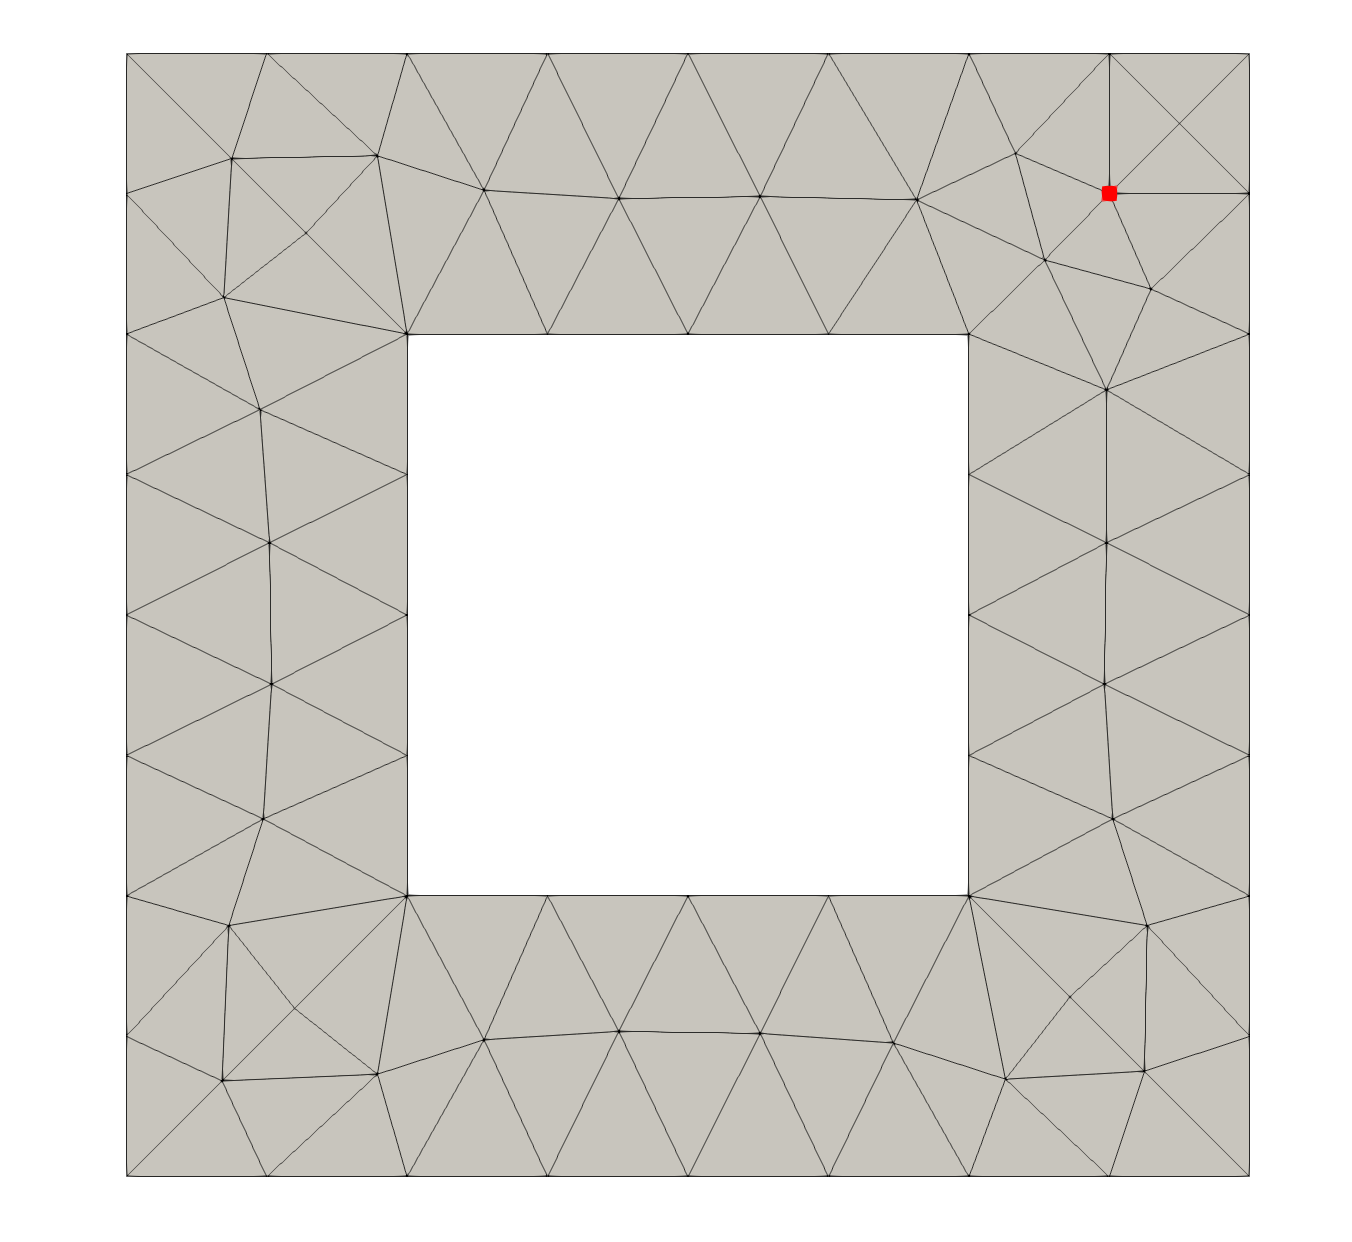
\includegraphics[width=.99\linewidth]{img/aut_squarehole_initial.png}
\end{subfigure}%
\begin{subfigure}{0.31\textwidth}
\centering
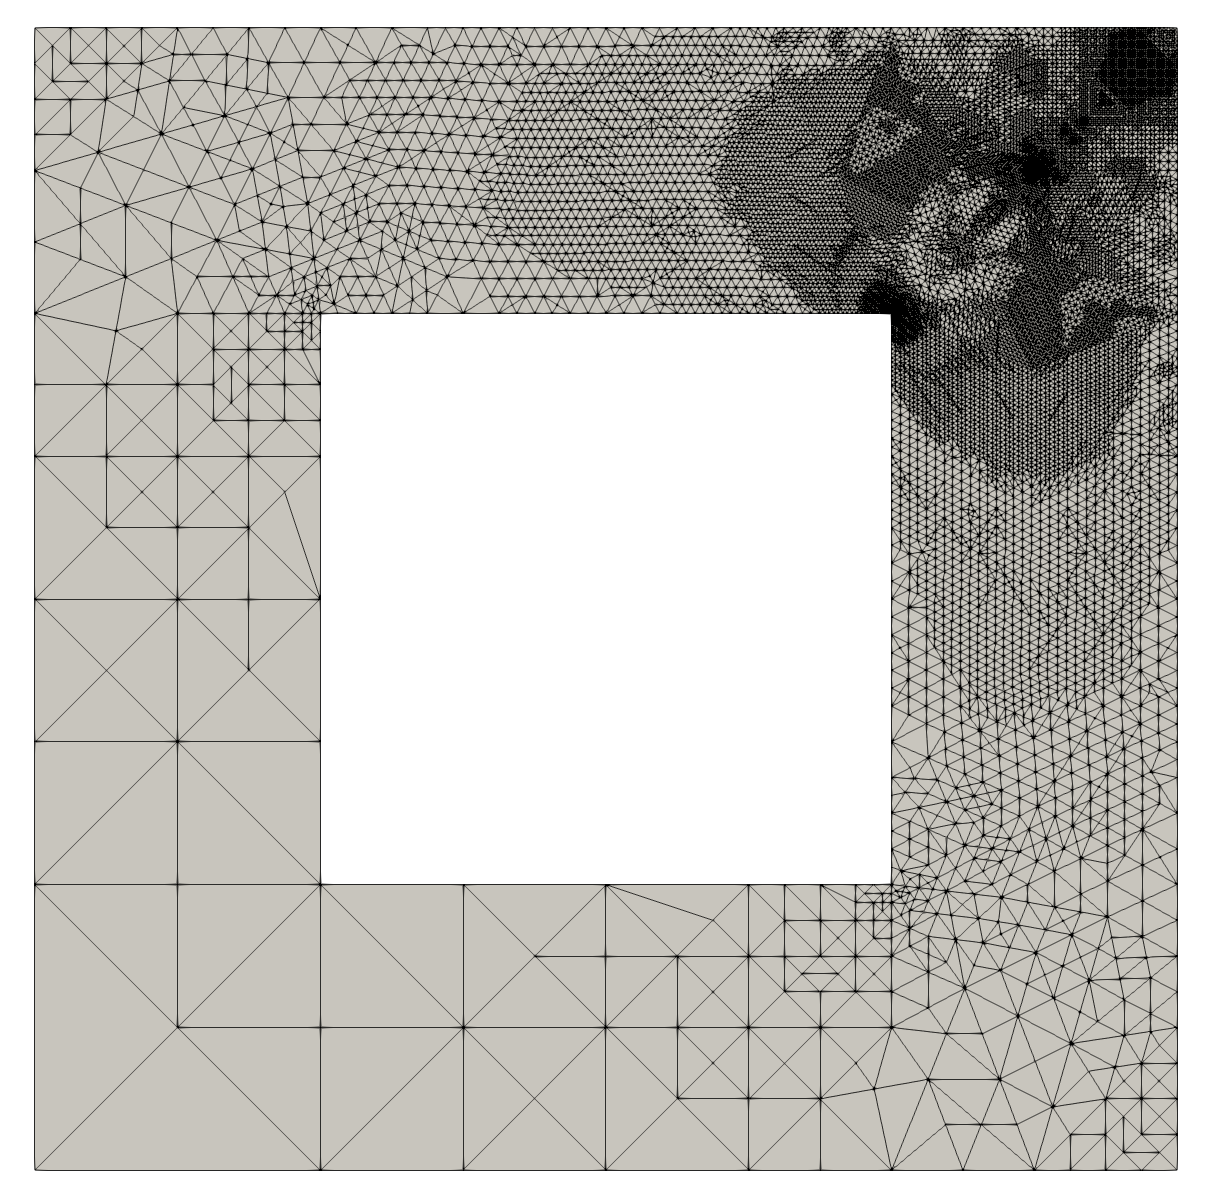
\includegraphics[width=.99\linewidth]{img/aut_squarehole_unif.png}
\end{subfigure}%
\begin{subfigure}{0.32\textwidth}
\centering
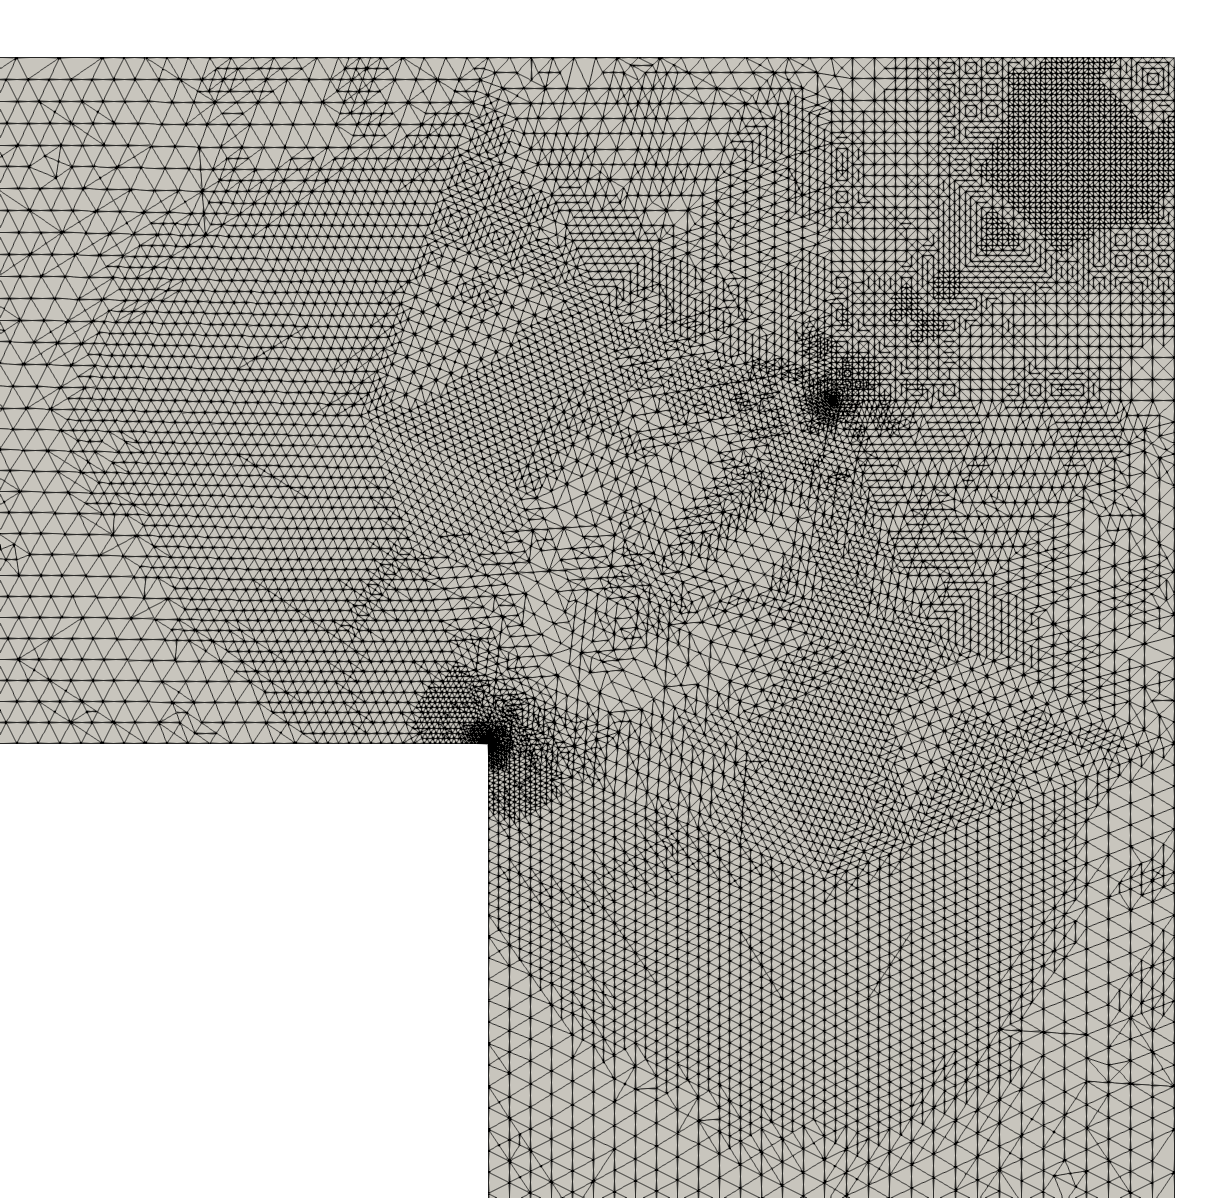
\includegraphics[width=.99\linewidth]{img/aut_squarehole_unif_close.png}
\end{subfigure}
\caption{Domain and initial mesh (left) for the Poisson's equation example
with the QoI point indicated in red, final adapted mesh (middle), and
a close up of the upper-right hand corner of the final adapted mesh (right).}
\label{fig:aut_poisson_meshes}
\end{figure}

Starting from the initial mesh shown in Figure \ref{fig:aut_poisson_meshes},
the steps:
%
\begin{gather*}
\text{Solve Primal} \rightarrow \text{Solve Adjoint} \rightarrow
\text{Estimate Error} \rightarrow \text{Adapt Mesh}
\end{gather*}
%
were performed seven times. The adaptive simulation was run using
4 MPI ranks. The mesh size field was set according to
equation \eqref{eq:aut_size_field} so that the target number of elements
is twice that of the current mesh. Figure \ref{fig:aut_poisson_meshes}
also shows the final adapted mesh resulting from this procedure. We remark
that the distribution of degrees of freedom in this mesh closely
resembles the results obtained in reference \cite{dealiistep14}.

%
%% aut_squarehole_effectivity
\begin{figure}[ht!]
\centering
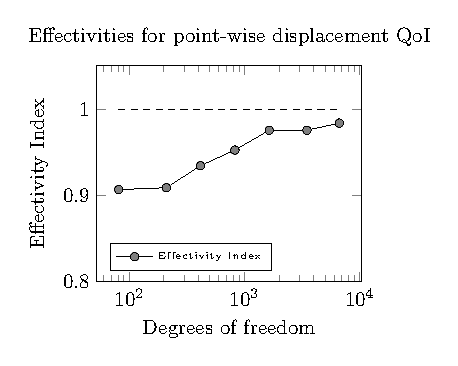
\includegraphics[width=.5\textwidth]{img/aut_squarehole_effectivity.pdf}
\caption{Effectivity indices for the adaptive Poisson's equation example.}
\label{fig:aut_squarehole_effectivity}
\end{figure}

We expect this functional to converge
at the rate $k=2$, such that the scaling factor $\alpha$ used in
the estimate \eqref{eq:aut_error_estimate} is given as
$\alpha = \frac34$. We consider the ``exact error''
$\E = J(u) - J(u^H)$ and the effectivity index
$\I = \frac{\eta}{\E}$, where $\eta$ is the estimate given by
equation \eqref{eq:aut_error_estimate}. Here we have placed quotations
around the term exact error because we have only approximated the
exact value of the QoI $J(u)$, and not truly recovered its exact value.
Figure \ref{fig:aut_squarehole_effectivity} plots the effectivity index
$\I$ versus the number of degrees of freedom in the adaptive
process. This plot demonstrates the ability of the error
estimate to recover the ``exact error'' as $H \to 0$.

%
%% aut_squarehole_error
\begin{figure}[ht!]
\centering
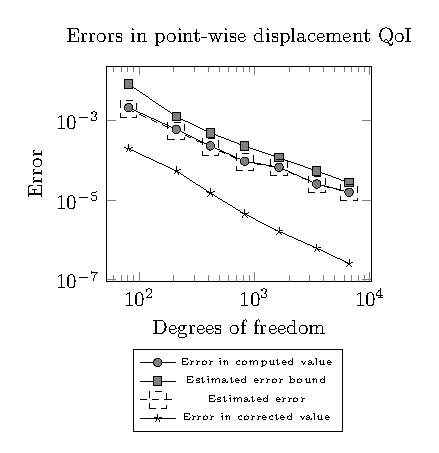
\includegraphics[width=.5\textwidth]{img/aut_squarehole_error.pdf}
\caption{Errors for the point-wise QoI for the adaptive Poisson's equation
example.}
\label{fig:aut_squarehole_error}
\end{figure}

Figure \ref{fig:aut_squarehole_error} displays the evolution of
various during the adaptive process. The ``exact error'' $\E$
and the estimated error $\eta$ are very close, as previously
demonstrated by the effectivity index $\I$. Additionally, the
approximated upper bound on the error $\hat{\eta}$ overestimates
the error, but not to a large degree. This provides some indication
that the correction indicators are effective in that they do
not drastically overestimate error. Finally, we remark that an
improved \emph{corrected} QoI functional value can be
computed as $J^*(u^H) = J(u^H) + \eta$. Figure
\ref{fig:aut_squarehole_error} demonstrates that this corrected
value is nearly an order of magnitude more accurate than
the computed functional value $J(u^H)$ during the adaptive process.

%
%% aut_squarehole_convergence
\begin{figure}[ht!]
\centering
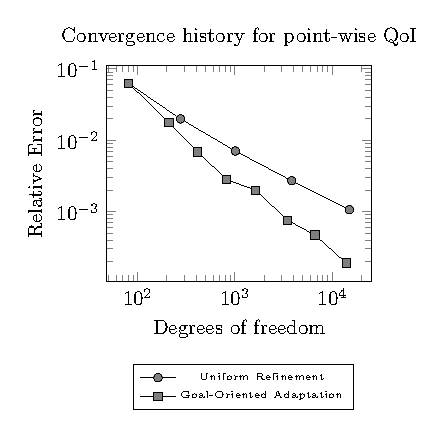
\includegraphics[width=.5\textwidth]{img/aut_squarehole_convergence.pdf}
\caption{Error convergence using uniform mesh refinement and adjoint-based
error estimation for the adaptive Poisson's equation example.}
\label{fig:aut_squarehole_convergence}
\end{figure}

Finally, Figure \ref{fig:aut_squarehole_convergence} demonstrates the
evolution of the ``exact error'' for two adaptive strategies.
The first strategy uniformly refines the mesh at each adaptive
step and the second strategy performs the adjoint-based adaptive scheme
developed in this work. We note that the error for the adjoint-based
adaptive scheme converges faster than the uniform refinement scheme.
Further, this convergence plot is consistent with the reference
\cite{dealiistep14}. 

%%% NONLINEAR ELASTICITY
\subsection{A Cell Embedded in a Matrix}

Recently, the automated approach developed in this paper was applied
to a stabilized mixed pressure-displacement finite element formulation
\cite{ramesh2005stabilized} for the governing equations of finite
deformation elasticity in a total Lagrangian setting
\cite{granzow2017adjoint} (see Chapter \ref{chap:mech}).
For two and three dimensional problems in
nonlinear elasticity, the automated approach was shown to effectively
estimate the error and provide improved error convergence rates via
adjoint-based mesh adaptation over uniform refinement.

In this section, the parallelization of a biomechanical application
presented in the reference \cite{granzow2017adjoint} is discussed. First,
the governing equations are briefly reviewed. For mixed pressure-displacement
formulations in the Goal application, the Galerkin residual is
defined as:
%
%% aut_mech_galerkin
\begin{gather}
\begin{aligned}
&\R_g(\bs{W}^H ; \bs{U}^H) := \\
&\int_{\Omega} \bs{P} : \nabla \bs{w}^H \, \text{d} \Omega +
\int_{\Omega} \left[ \frac{p^H}{\kappa} - \frac{1}{2 J}(J^2 - 1) \right] \;
q^H \, \text{d} \Omega -
\int_{\partial \Omega_h} \bs{h} \cdot \bs{w} \; \text{d} \Gamma,
\end{aligned}
\label{aut:mech_galerkin}
\end{gather}
%
and the stabilization residual is defined as:
%
%% aut_mech_stabilized
\begin{gather}
\R_{\tau}(\bs{W}^H ; \bs{U}^H) :=
\sum_{e=1}^{n_{el}} \int_{\Omega_e} \tau_e
(J \bs{F}^{-1} \bs{F}^{-T}) : (\nabla p^H \otimes \nabla q^H) \;
\text{d} \Omega.
\label{aut_mech_stabilized}
\end{gather}
%
Here, $\bs{F}$ is the deformation gradient, $J := \text{det}(\bs{F})$,
$\bs{h}$ is an applied traction over the boundary $\partial \Omega_h$,
$\bs{P} := J \bs{\sigma} \bs{F}^{-T}$ is the first Piola-Kirchhoff
stress tensor, $\bs{\sigma}$ is the Cauchy stress tensor, $n_{el}$
is the total number of elements in the mesh, and $\tau_e :=
\frac{c_0 H_e^2}{2 \mu}$ is a mesh-dependent stabilization parameter,
where $c_0$ is a non-negative stability constant, $H_e$ denotes an
element mesh size and $\mu$ denotes the bulk modulus.
The Cauchy stress tensor is defined via a neo-Hookean constitutive
relationship.  The total
solution vector is defined as $\bs{U}^H := [\bs{u}^H, p^H]$, where
$\bs{u}^H$ corresponds to displacements and $p^H$ corresponds to
pressures. Similarly, the total weighting vector is defined as
$\bs{W}^H := [\bs{w}^H, q^H]$, where $\bs{w}^H$ denotes a weighting
function corresponding to displacements and $q^H$ is a weighting
function corresponding to pressures. For a complete
exposition, we refer the reader to Chapter \ref{chap:mech}.

%
%% aut_glial_geom
\begin{figure}[ht!]
\centering
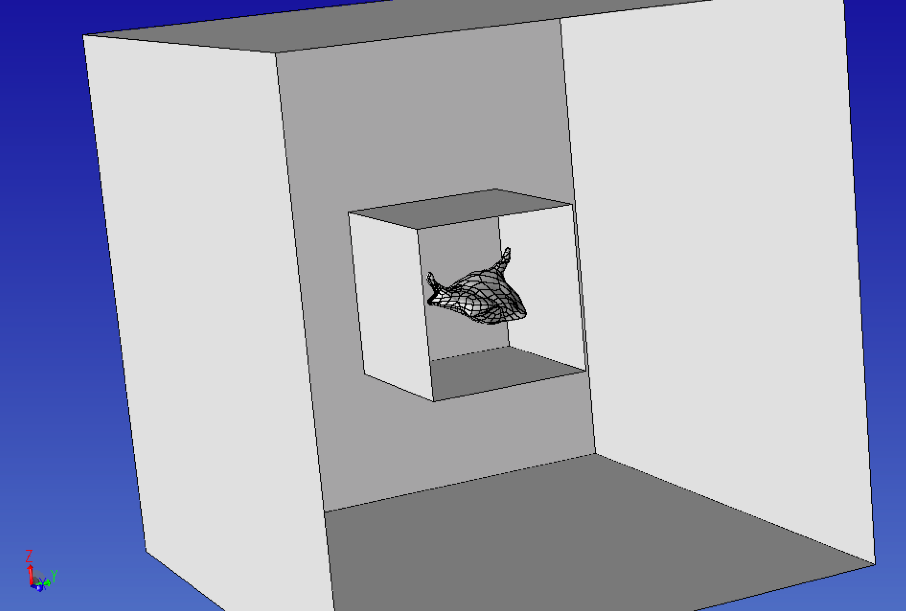
\includegraphics[width=.5\linewidth]{img/aut_glial_geom.png}
\caption{Domains for the microglial cell example.}
\label{fig:aut_glial_geom}
\end{figure}

We focus on a microglial cell with dimensions of about
$20 \mu m \times 20 \mu m \times 20 \mu m$ embedded in an extracellular
matrix of dimension $100 \mu \times 100 \mu m \times 100 \mu m$.
The QoI is chosen to be a local average displacement
$J(\bs{U}) = \int_{\Omega_0} \frac13 (u_x + u_y + u_z) \, \text{d} \Omega$,
defined over a box $\Omega_0$ with dimensions
$30 \mu m \times 30 \mu m \times 30 \mu m$
that bounds the microglial cell. Figure \ref{fig:aut_glial_geom} shows
the geometry defining the microglial cell, the bounding box
$\Omega_0$, and the extracellular matrix. The shear modulus
is defined as $\mu = 600$ Pa and Poisson's ratio is set to be
$\nu = 0.4999$.

To drive the problem, traction boundary conditions are imposed along
the surface of the microglial cell. The magnitude of the applied
traction $\bs{h}$ is defined to be 10 times the distance to the
center of the cell and its direction points inward towards the
cell center. This traction is consistent with observed physical
behavior \cite{dong2017recovery}. Displacements $u_x = 0$,
$u_y=0$, and $u_z=0$ are applied to the faces with constant
minimum $x$-coordinate value, constant minimum $y$-coordinate
value, and constant minimum $z$-coordinate value, respectively,
to constrain rigid body rotations and translations.

%
%% aut_glial_meshes
\begin{figure}[ht!]
\centering
\begin{subfigure}{.33\textwidth}
\centering
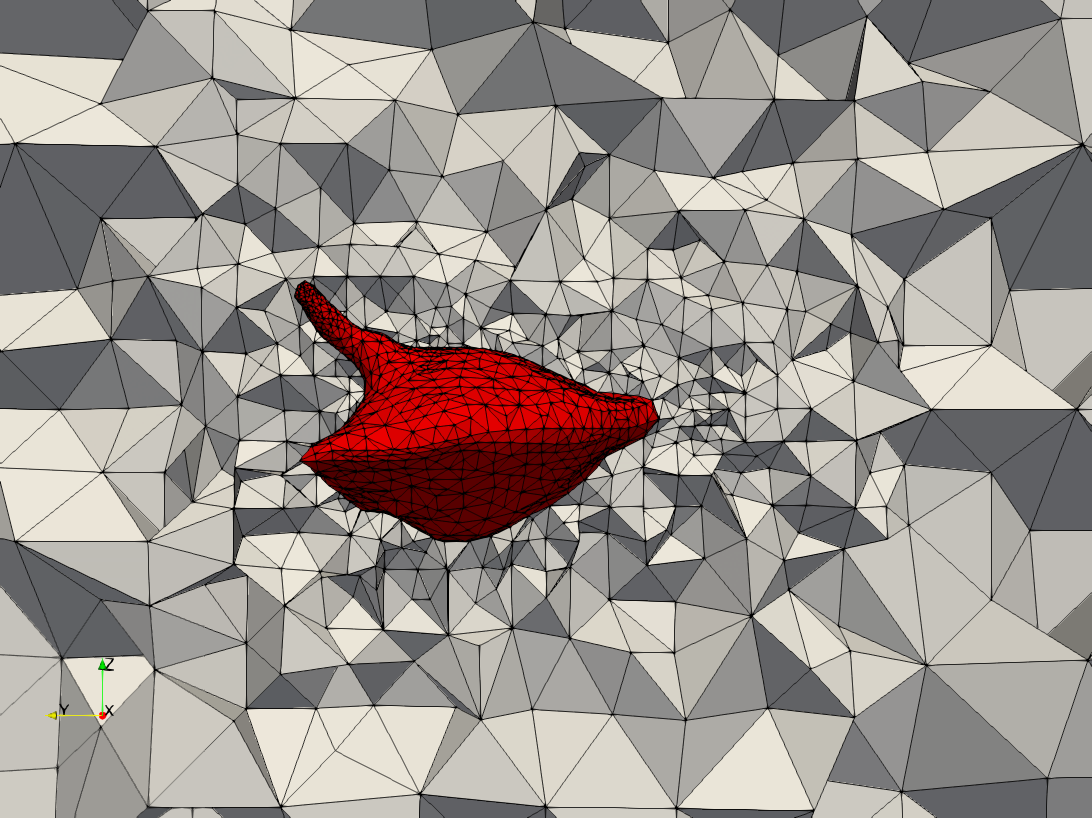
\includegraphics[width=.99\linewidth]{img/aut_glial_mesh0.png}
\end{subfigure}%
\begin{subfigure}{0.33\textwidth}
\centering
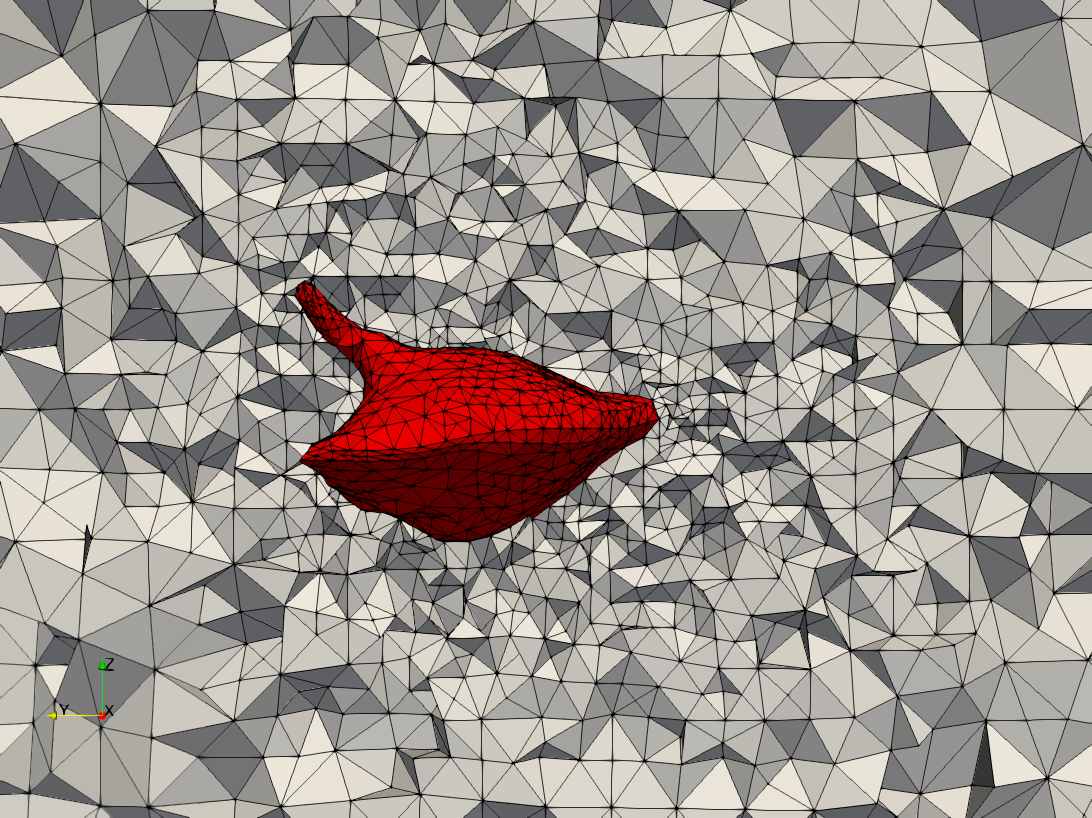
\includegraphics[width=.99\linewidth]{img/aut_glial_mesh5.png}
\end{subfigure}%
\begin{subfigure}{0.33\textwidth}
\centering
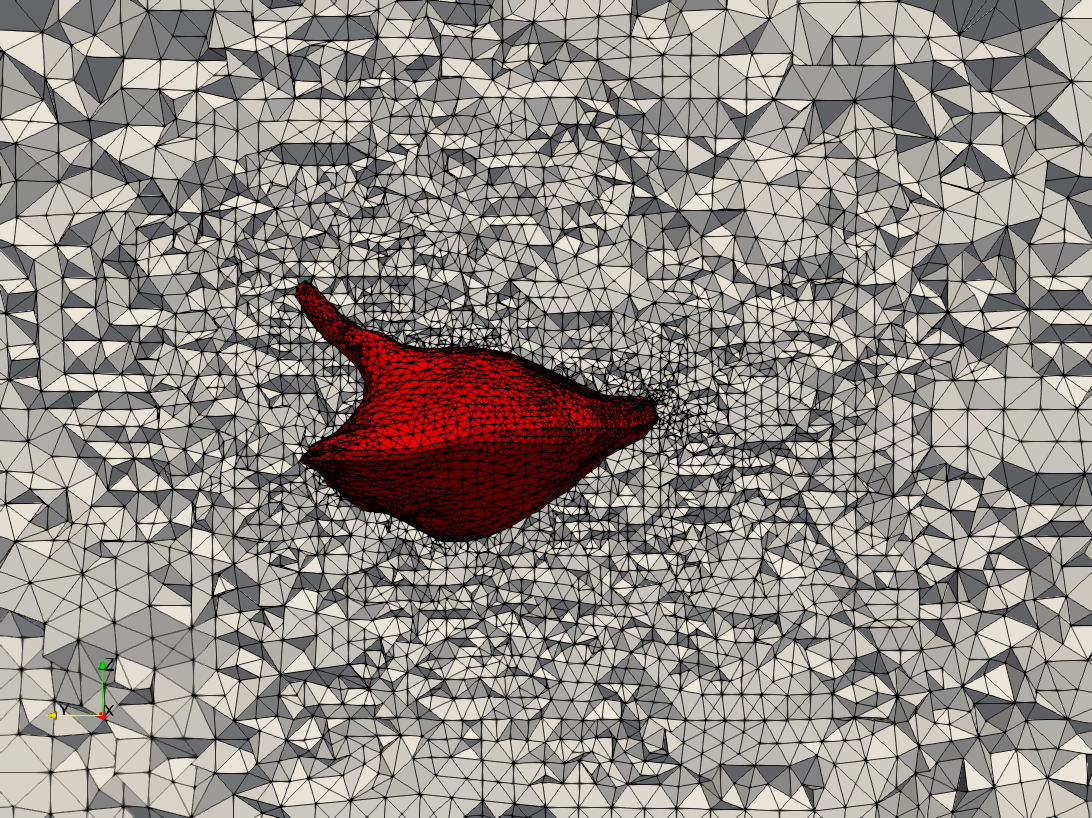
\includegraphics[width=.99\linewidth]{img/aut_glial_mesh10.png}
\end{subfigure}
\caption{A close-up of the initial mesh (left) the mesh after
5 adaptive iterations (center) and the final adapted mesh (right)
for the microglial cell example}
\label{fig:aut_glial_meshes}
\end{figure}

Figure \ref{fig:aut_glial_meshes} demonstrates an initial mesh,
which contains around $30,000$ degrees of freedom. From this initial
mesh, the steps
%
\begin{gather*}
\text{Solve primal PDE} \rightarrow
\text{Solve adjoint PDE} \rightarrow
\text{Localize error} \rightarrow
\text{Adapt mesh}
\end{gather*}
%
were successively performed $10$ times. During the adapt stage,
the mesh size field was set such that desired number of elements
$N$ in the output mesh is $1.5$ times the number of elements
in the previous mesh, according to equation \eqref{eq:aut_size_field}.
Figure \ref{fig:aut_glial_meshes} additionally demonstrates the adapted
meshes obtained at the fifth and final adaptive iteration.
In particular, both \emph{coarsening} and \emph{refinement} is performed
during the adaptive iterations.

\begin{figure}[ht!]
\centering
\begin{subfigure}{.5\textwidth}
\centering
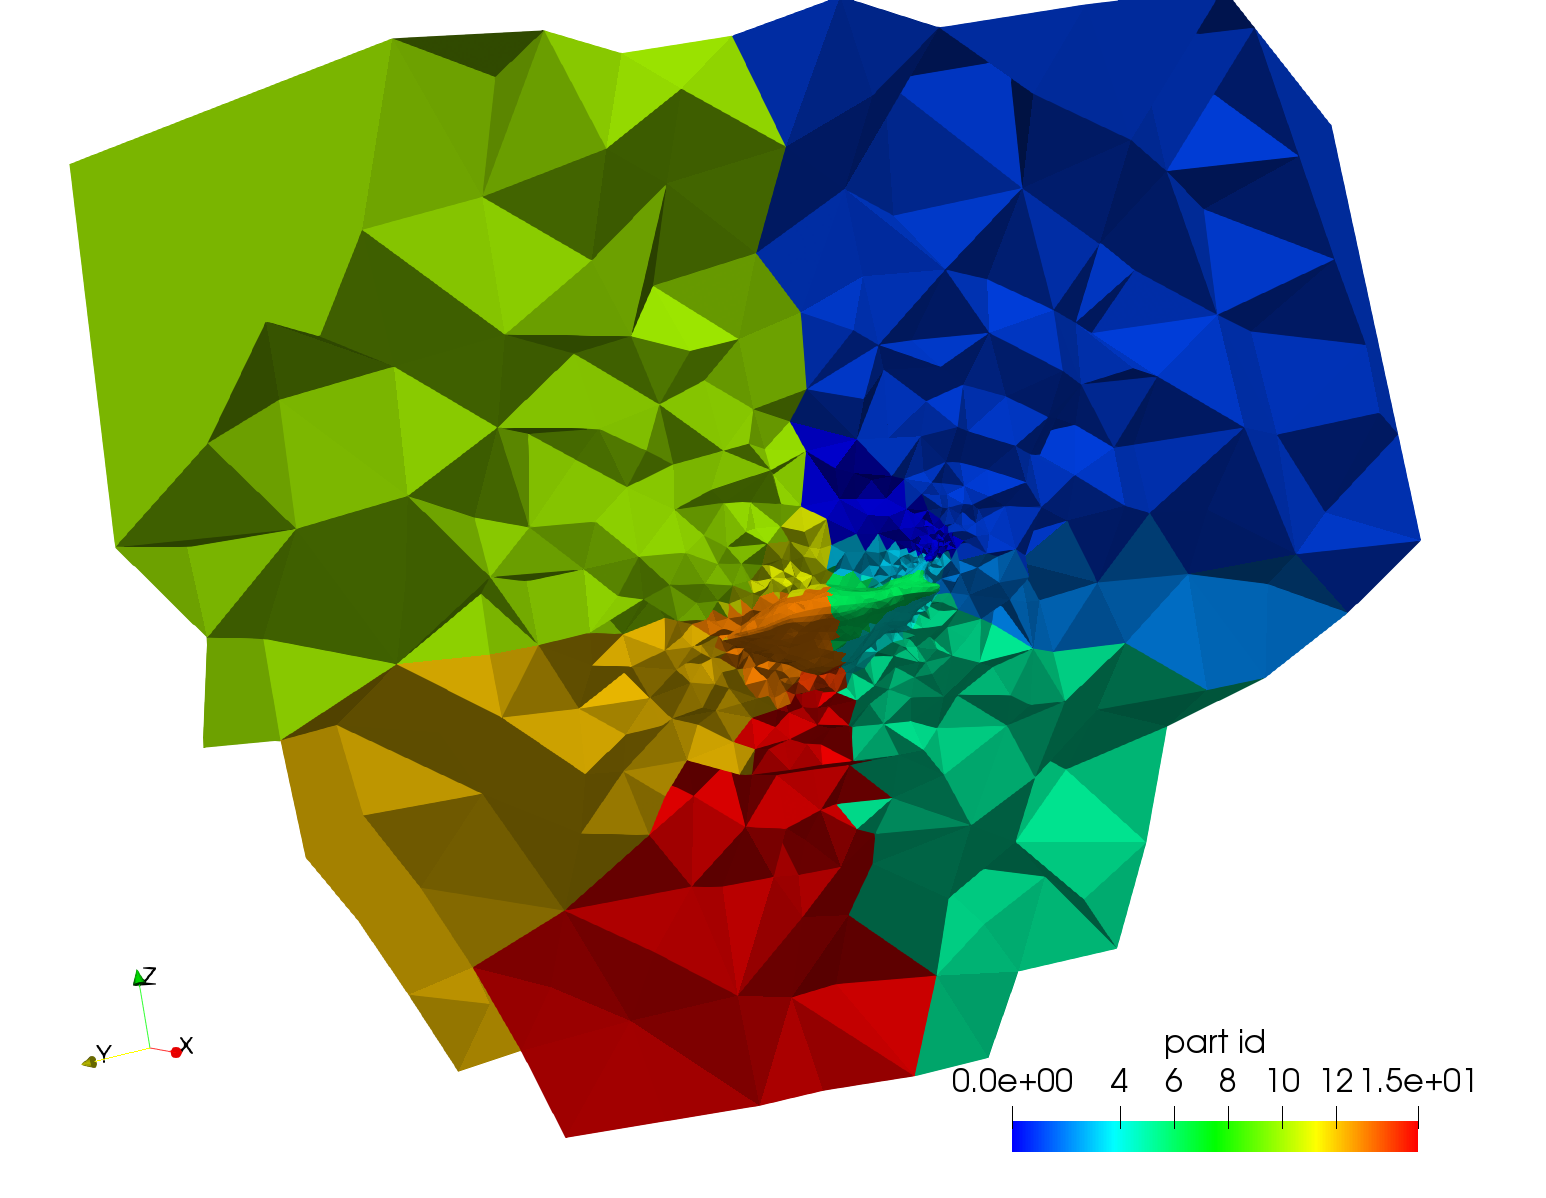
\includegraphics[width=.99\linewidth]{img/aut_glial_initial_parts.png}
\end{subfigure}%
\begin{subfigure}{0.5\textwidth}
\centering
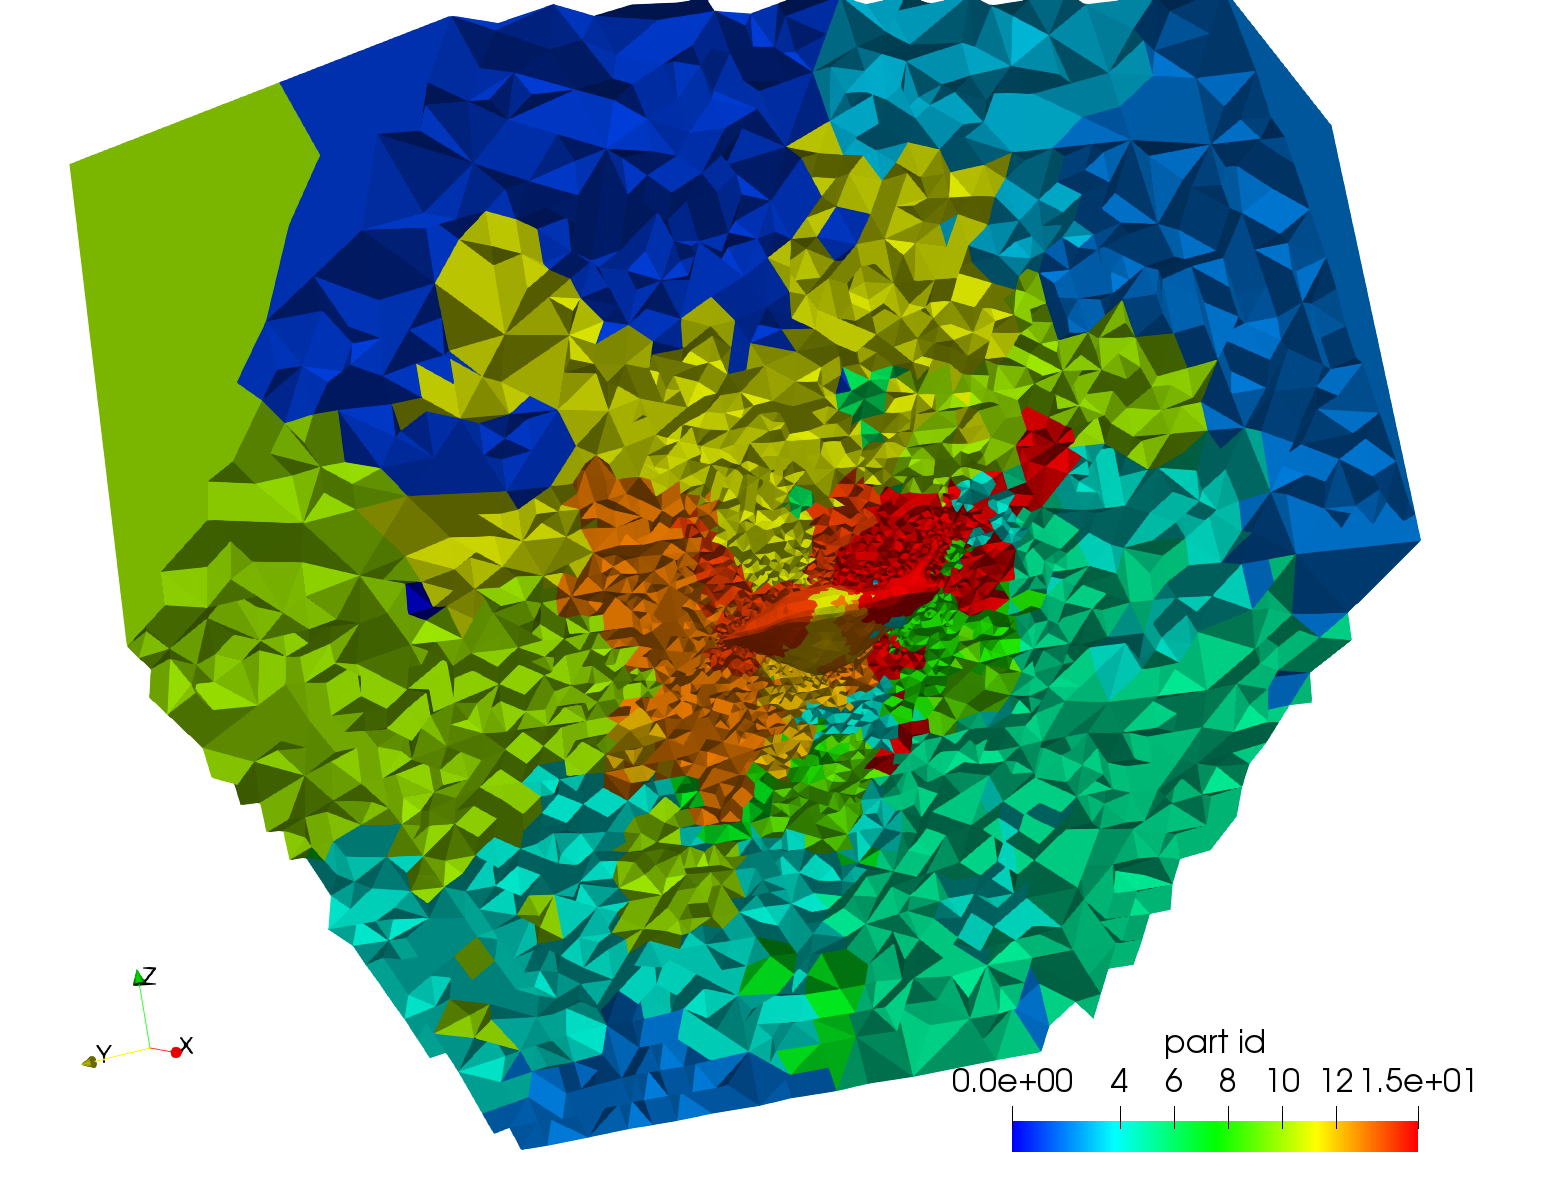
\includegraphics[width=.99\linewidth]{img/aut_glial_final_parts.png}
\end{subfigure}
\caption{The parallel mesh partitioning for the initial mesh (left)
and the final adapted mesh (right) for the microglial cell example}
\label{fig:aut_glial_parts}
\end{figure}

The problem was run using 16 MPI ranks. Figure \ref{fig:aut_glial_parts}
demonstrates the parallel partitioning for the initial mesh and for
the final adapted mesh obtained after 10 adjoint-based adaptive
iterations. To ensure partitioning quality, ParMA was
utilized to guarantee the imbalance of vertices and elements
across parallel partitions is no greater than $5\%$.

\begin{figure}[ht!]
\centering
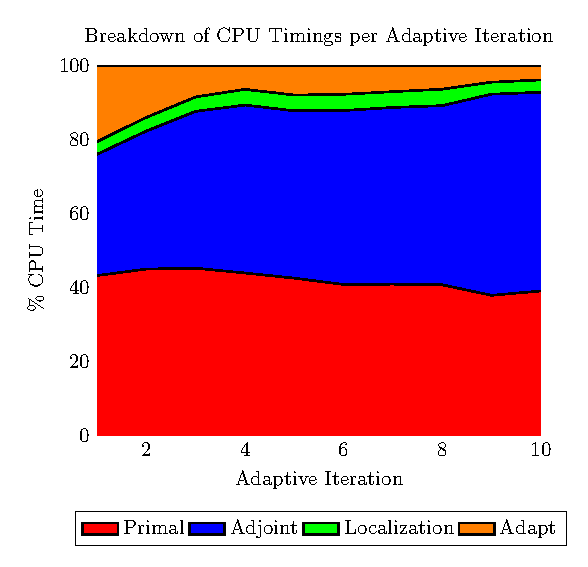
\includegraphics[width=0.4\linewidth]{img/aut_glial_timings.pdf}
\caption{Breakdown of the CPU time spent for each portion of
the adaptive process for the microglial cell example}
\label{fig:aut_glial_timings}
\end{figure}

Figure \ref{fig:aut_glial_timings} presents a breakdown of the
total percentange of CPU time spent on each step in the
adaptive analysis. For every adaptative iteration, the error
localization \eqref{eq:aut_stabilized_localization} takes only
a small percentage of the total CPU time, as it essentially amounts
to an evaluation of the residual vector the fine space. More
interestingly, mesh adaptation initially accounts for about
20 percent of the total CPU time but decreases as the adaptive
simulation progresses. This is explained by the fact that the initial
adaptive iteration requires more work to optimally distribute
the degrees of freedom for the functional QoI as compared to
subsequent adaptive iterations. In addition to refinement
and coarsening operations, the mesh adaptation step also
performs \emph{shape correction} to ensure elements are not
too heavily skewed \cite{li20053d}. Finally, we note that the
adjoint problem accounts for roughly 40 to 50 percent of the CPU time
over the course of the adaptive simulation. While process of
adjoint-based error estimation is not cheap for this example,
we provide two justifying remarks. First, this problem required only
3 to 4 Newton iterations for each primal solve. For constitutive
models with higher degrees of nonlinearity or for problems loaded to
higher strains, it is not uncommon for Newton's method to converge
in 7 to 10 iterations. In these scenarios, the relative cost of
adjoint-based error estimation is not as extreme.
Second, for this computational price, we have
achieved very accurate error estimates as shown in
Chapter \ref{chap:mech}.

%%% ELASTOPLASTICITY IN AN ARRAY OF SOLDER BALLS
\subsection{Elastoplasticity in an Array of Solder Joints}

In this section, we investigate the utility of adjoint-based mesh
adaptation for a thermomechanical analysis of an array of solder
joints used in microelectronics fabrication. We consider a
$6 \times 6$ array of solder joints sandwiched between two materials
with distinct thermomechanical properties
to model a portion of the process of `flip-chip'
manufacturing \cite{bloomfield2017component}. The full geometry
is shown in Figure \ref{fig:aut_solder_geom}. We consider
an elastoplastic constitutive model with a von-Mises yield
surface and linear isotropic hardening, as given by
Simo and Hughes \cite{simo2006computational} with a temperature
correction for the stress tensor \cite{li2017simulation}. The top
slab, solder joints, and bottom slab are modeled with the
distinct material properties given in reference
\cite{bloomfield2017component}.

To drive the problem, the entirety of the domain is cooled
from a reference temperature $T_{ref} = 393K$ to a
resting temperature of $T_{f} = 318K$ in a single load
step. The faces with minimum $x$, $y$, and $z$ coordinate
values were constrained to have zero displacements in
the $x$, $y$, and $z$ directions, respectively. As a
QoI, we consider the average von-Mises stress given by
equation \eqref{eq:aut_avg_vm_qoi} over three solder joints
shown in yellow in Figure \ref{fig:aut_solder_geom}.

\begin{figure}[ht!]
\centering
\begin{subfigure}{.5\textwidth}
\centering
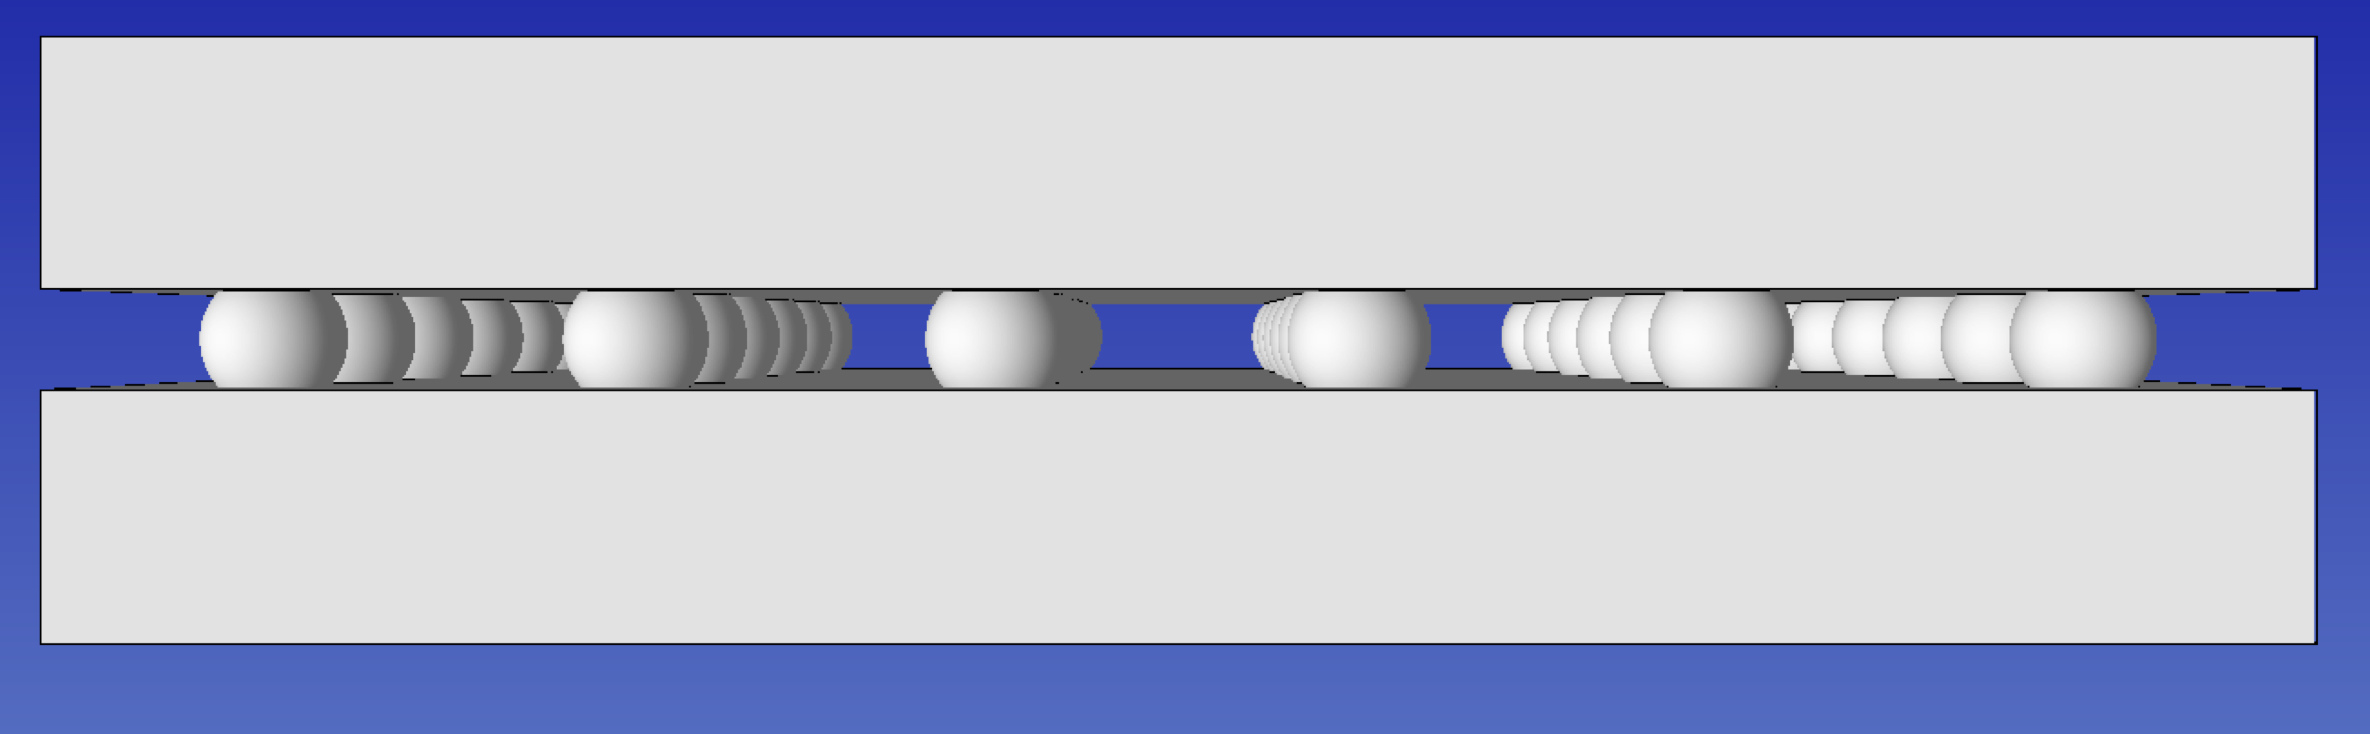
\includegraphics[width=.99\linewidth]{img/aut_solder_geom.png}
\end{subfigure}%
\begin{subfigure}{0.5\textwidth}
\centering
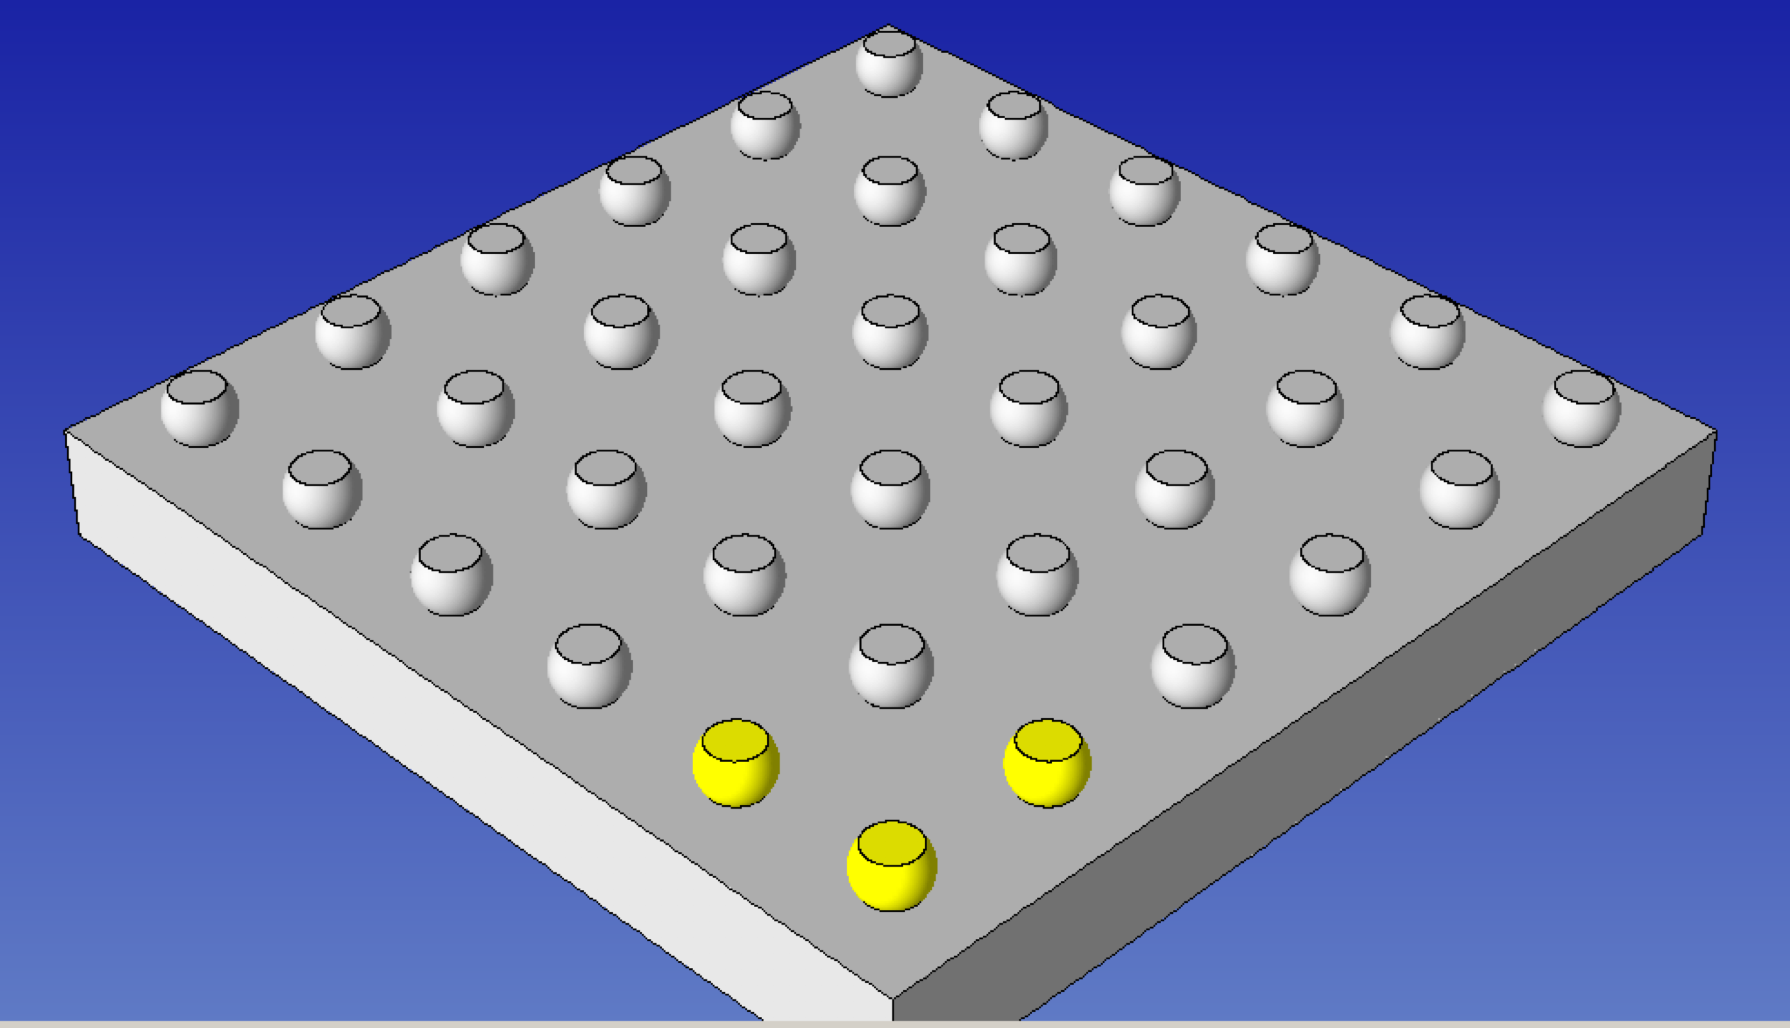
\includegraphics[width=.99\linewidth]{img/aut_solder_qoi_geom.png}
\end{subfigure}
\caption{The solder joint array geometry (left) and the
geometric specification of the average von-Mises QoI
(right).}
\label{fig:aut_solder_geom}
\end{figure}

The primal problem was solved on a sequence of uniformly refined
meshes, starting with an initial mesh with about 1 million
elements distributed over 16 MPI ranks, and finalizing with a
mesh with over half a billion elements distributed over
8192 MPI ranks. For each solve, the work load for each mesh
part (MPI rank) was held constant at approximately
$70,000$ elements. Figure \ref{fig:aut_weak_scaling}
demonstrates weak scaling timing results for various aspects
of the primal solve. In particular, we remark that the
assembly of the residual vector and Jacobian matrix scale
well as the number of MPI ranks increases. The preconditioning
routine shows a slight increase in time as the number of
MPI ranks increases, but this increase is not drastic.
The time to solve the linear system, however, does not scale
optimally. Improvements to parallel performance could likely
be made by more finely tuning the preconditioning and linear
solver routines for the specific problem, but this is outside
the scope of the present work.

\begin{figure}[ht!]
\centering
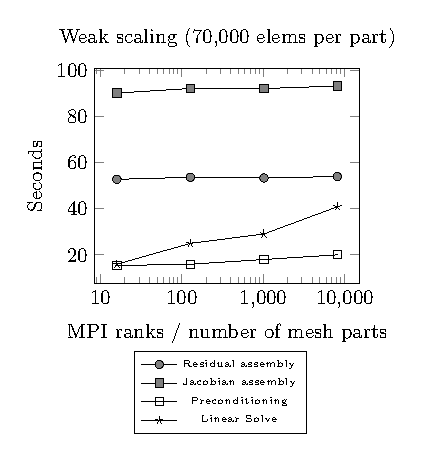
\includegraphics[width=0.5\linewidth]{img/aut_weak_scaling.pdf}
\caption{Weak scaling for the Goal application.}
\label{fig:aut_weak_scaling}
\end{figure}

The approximate QoI, $J^H(\bs{u}^H)$, was computed at each
primal solve. Using the QoI evaluations from the finest three meshes,
we performed Richardson extrapolation \cite{richardson1911approximate}
to obtain a more accurate representation of the QoI.
This value was given as $J(u) = 328.9$. We consider the extrapolated
value to be the ``true'' QoI value and measure errors with respect
to it. The expected convergence rate of the QoI is $k=1$, which is
confirmed by the Richardson extrapolation procedure.

\begin{figure}[ht!]
\centering
\begin{subfigure}{.33\textwidth}
\centering
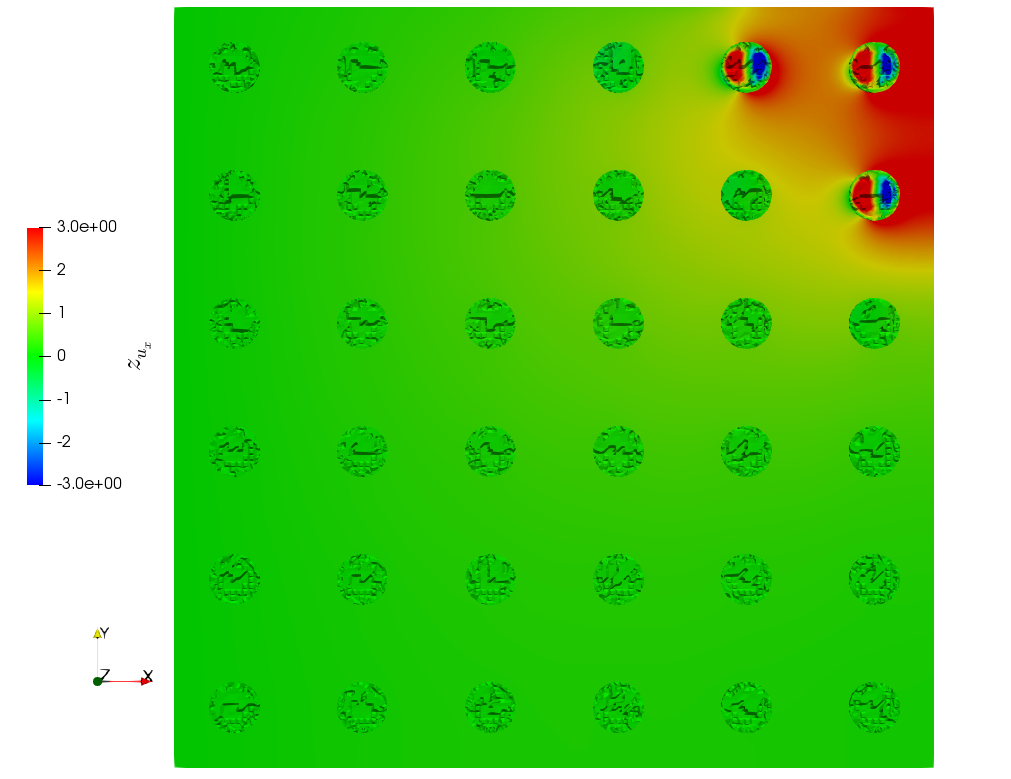
\includegraphics[width=.99\linewidth]{img/aut_solder_zux.png}
\end{subfigure}%
\begin{subfigure}{0.33\textwidth}
\centering
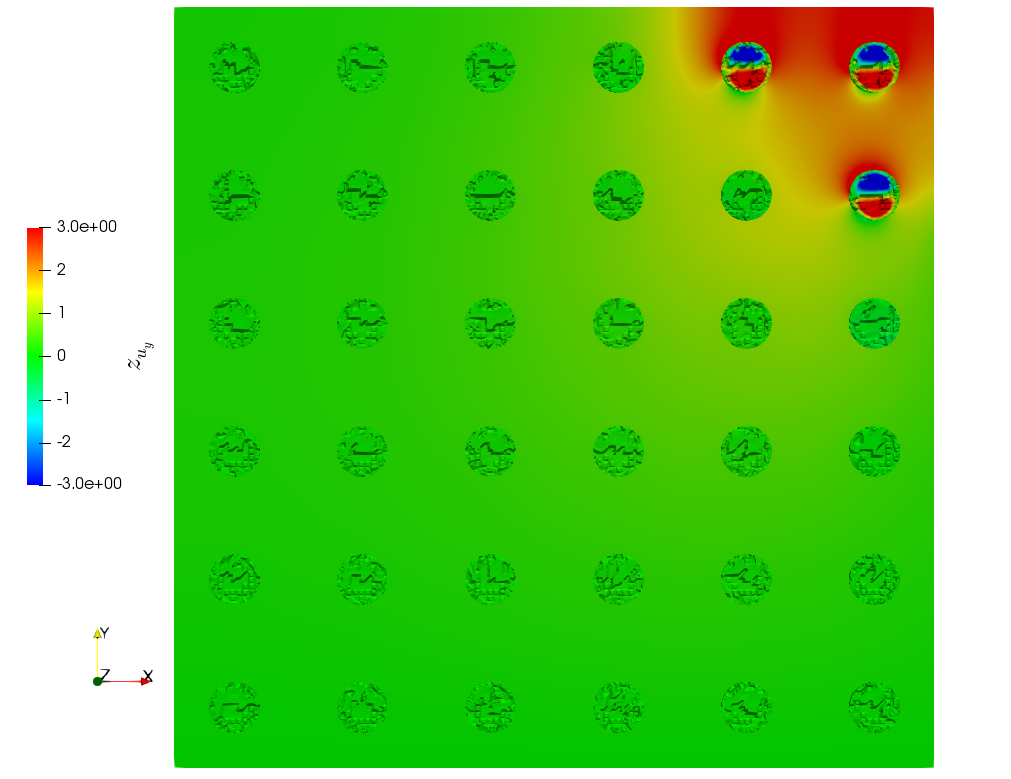
\includegraphics[width=.99\linewidth]{img/aut_solder_zuy.png}
\end{subfigure}%
\begin{subfigure}{0.33\textwidth}
\centering
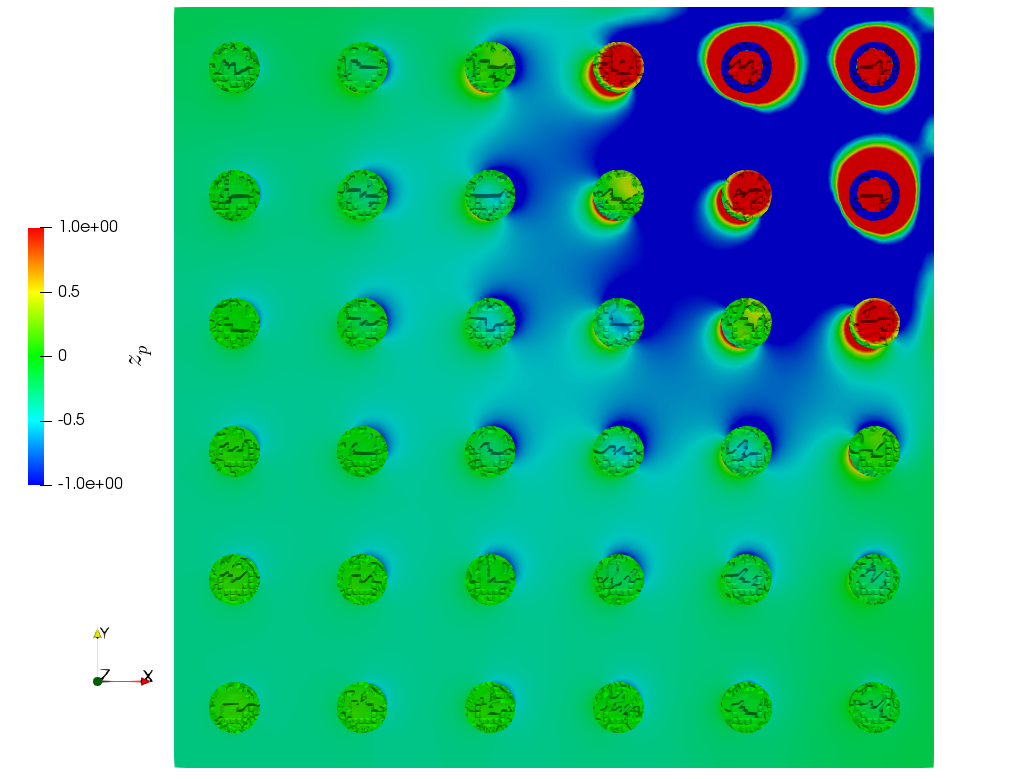
\includegraphics[width=.99\linewidth]{img/aut_solder_zp.png}
\end{subfigure}
\caption{The $x$-component of the adjoint displacement solution
(left), the $y$-component of the adjoint displacement solution
(center), and the pressure component of the adjoint solution
(right).}
\label{fig:aut_solder_adjoint}
\end{figure}

From the same initial mesh used in the weak scaling study,
we iteratively performed the steps:
%
\begin{gather*}
\text{Solve Primal} \rightarrow \text{Solve Adjoint} \rightarrow
\text{Estimate Error} \rightarrow \text{Adapt Mesh}
\end{gather*}
%
with a restart after each mesh adaptation using $128$,
$256$, and $512$ MPI ranks, such that the output number
of elements $N$ in the adapted mesh was targeted to be
$1$ million, $2$ million, and $4$ million elements,
respectively. Figure \ref{fig:aut_solder_adjoint} shows
different components of the adjoint solution obtained
during the adjoint-based adaptive process.
Figure \ref{fig:aut_solder_error} shows
the spatial distribution of the error for the given
QoI as computed by the adjoint-based error estimation process.
Unsurprisingly, the majority of the error is localized to the
area which geometrically defines the QoI. However, there are
also contributions to the error from nearby solder joints that
decrease as the distance from the 3 QoI solder joints
increases. These additional contributions to the error
are mostly gathered at the interface between solder
joints and the underlying material slab, where von-Mises
stress concentrations exist.

\begin{figure}[ht!]
\centering
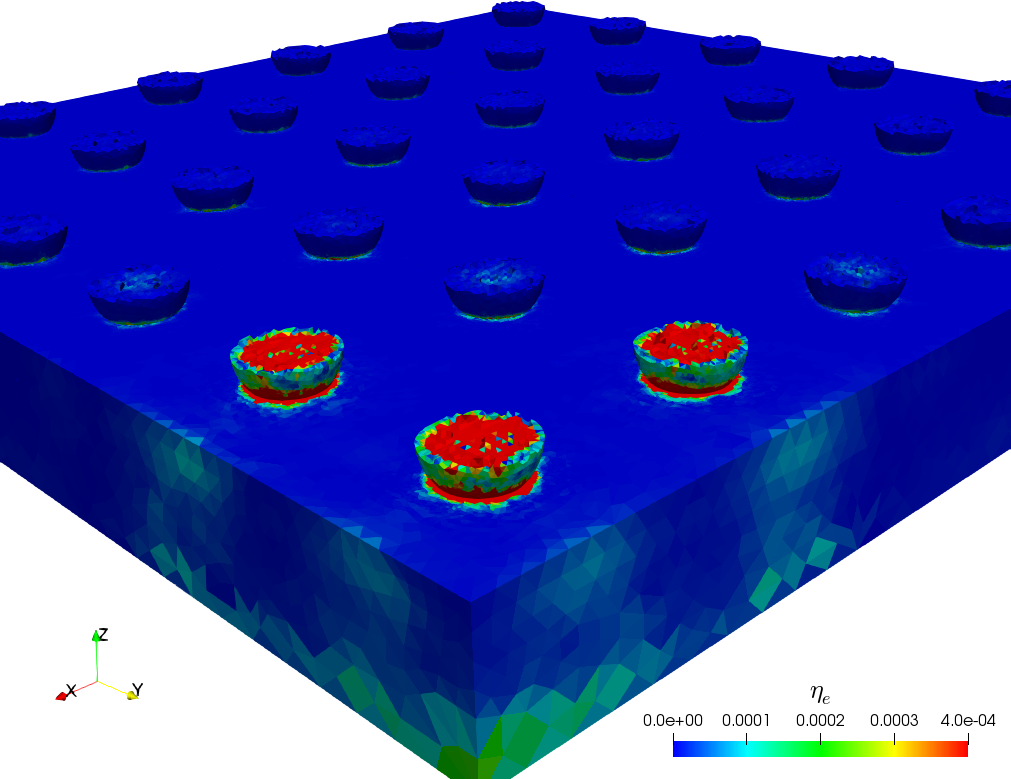
\includegraphics[width=.5\linewidth]{img/aut_solder_error.png}
\caption{The spatial distribution of errors as computed by
adjoint-based error estimation for the solder joint array.}
\label{fig:aut_solder_error}
\end{figure}

Figures \ref{fig:aut_solder_mesh} and \ref{fig:aut_solder_mesh2}
demonstrate the intial mesh used for the solder joint problem
and the final adapted mesh obtained via adjoint-based adaptation.
These figures clearly demonstrate that the 3 solder joints
that define the QoI sub-domain are heavily refined, as expected.
Additionally, notice that Figure \ref{fig:aut_solder_mesh}
demonstrates that there is refinement at the left-most solder joint,
which is not included in the geometric definition of the QoI.
The adjoint-based error estimation procedure indicates that
mesh must be refined in additional areas to accurately assess
the QoI.

\begin{figure}[ht!]
\centering
\begin{subfigure}{.5\textwidth}
\centering
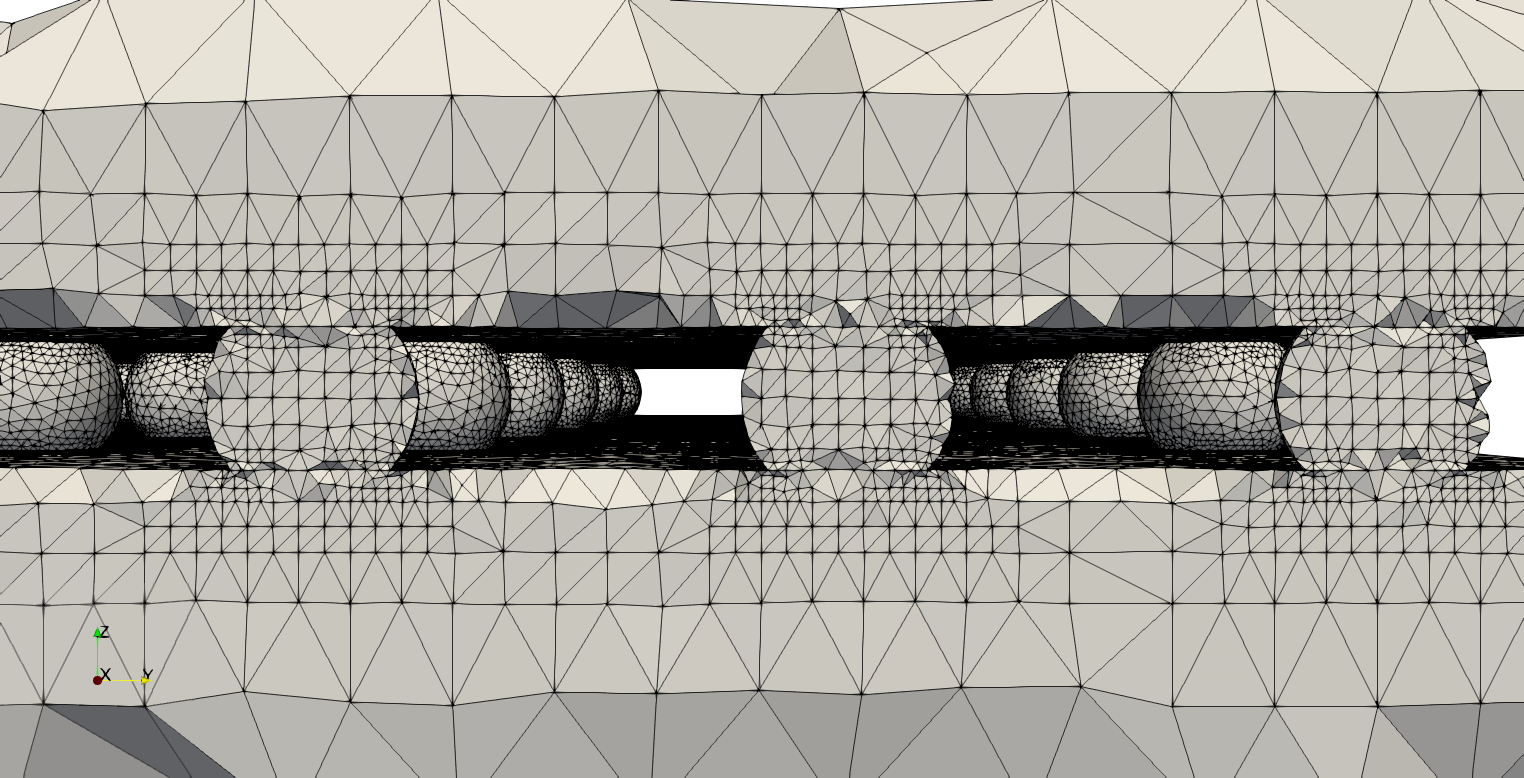
\includegraphics[width=.99\linewidth]{img/aut_solder_mesh_initial.png}
\end{subfigure}%
\begin{subfigure}{0.5\textwidth}
\centering
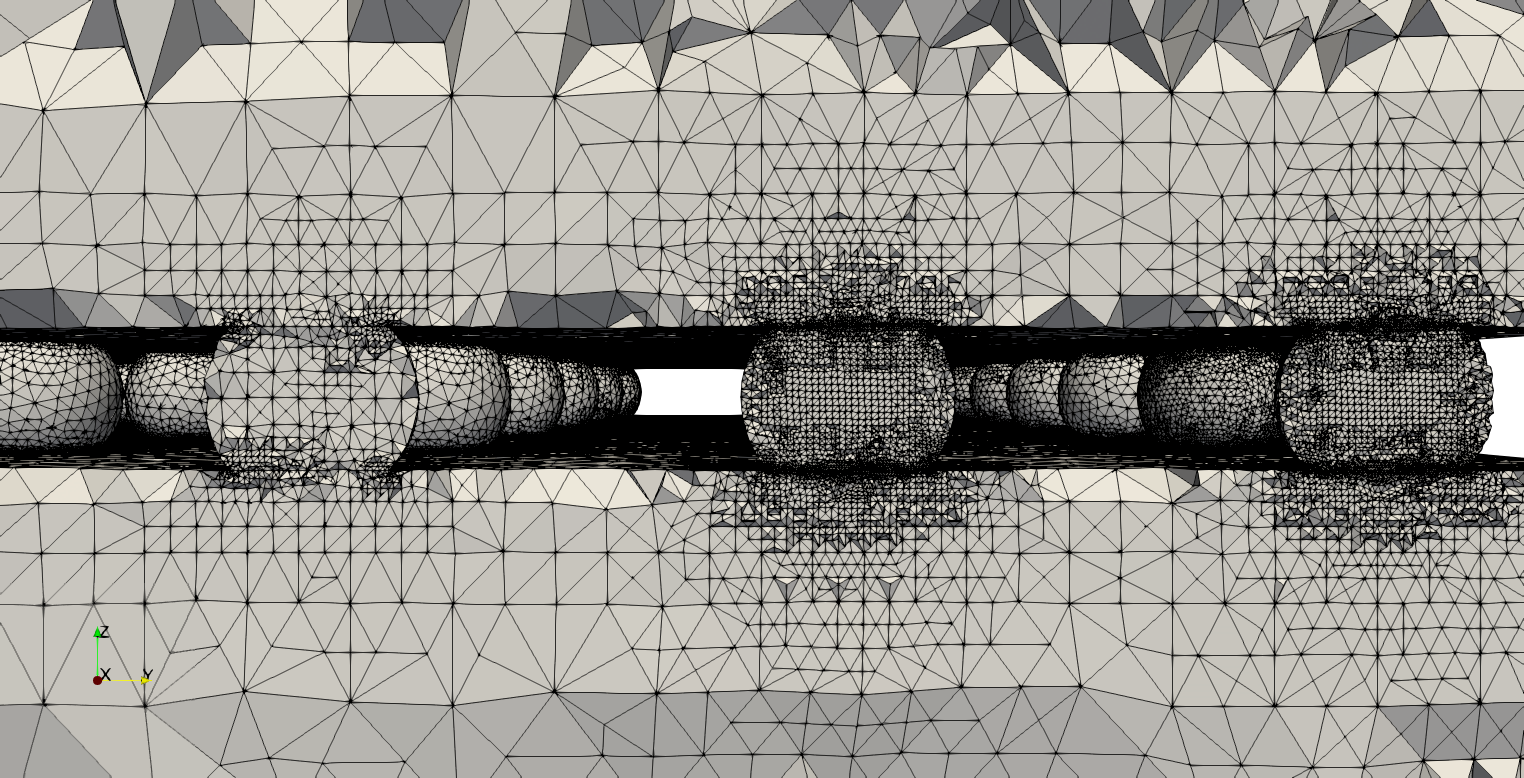
\includegraphics[width=.99\linewidth]{img/aut_solder_mesh_final.png}
\end{subfigure}%
\caption{Cross-sectional view of the initial mesh for the solder joint
geometry (left) and the final adapted mesh (right).}
\label{fig:aut_solder_mesh}
\end{figure}

\begin{figure}[ht!]
\centering
\begin{subfigure}{.5\textwidth}
\centering
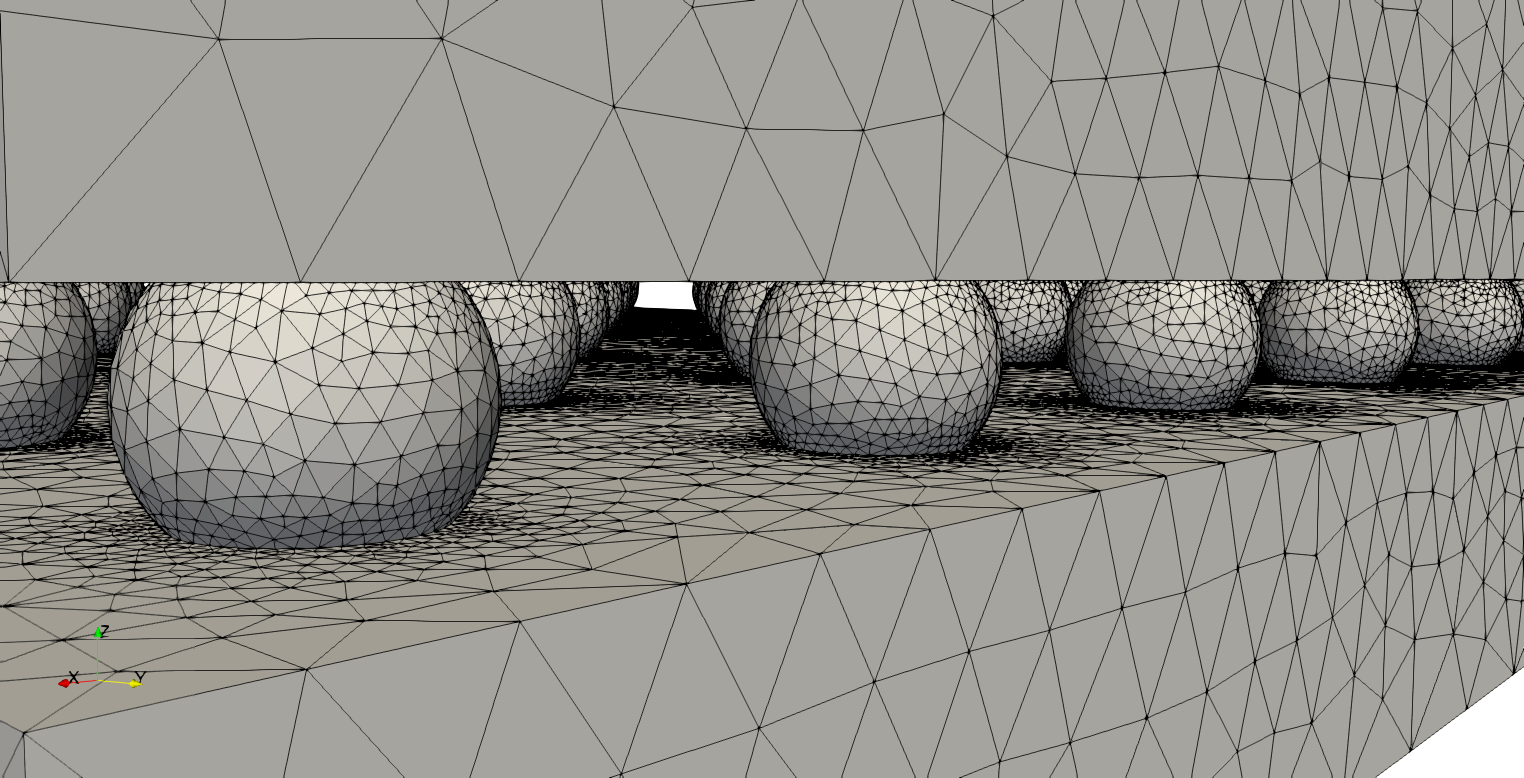
\includegraphics[width=.99\linewidth]{img/aut_solder_mesh_initial2.png}
\end{subfigure}%
\begin{subfigure}{0.5\textwidth}
\centering
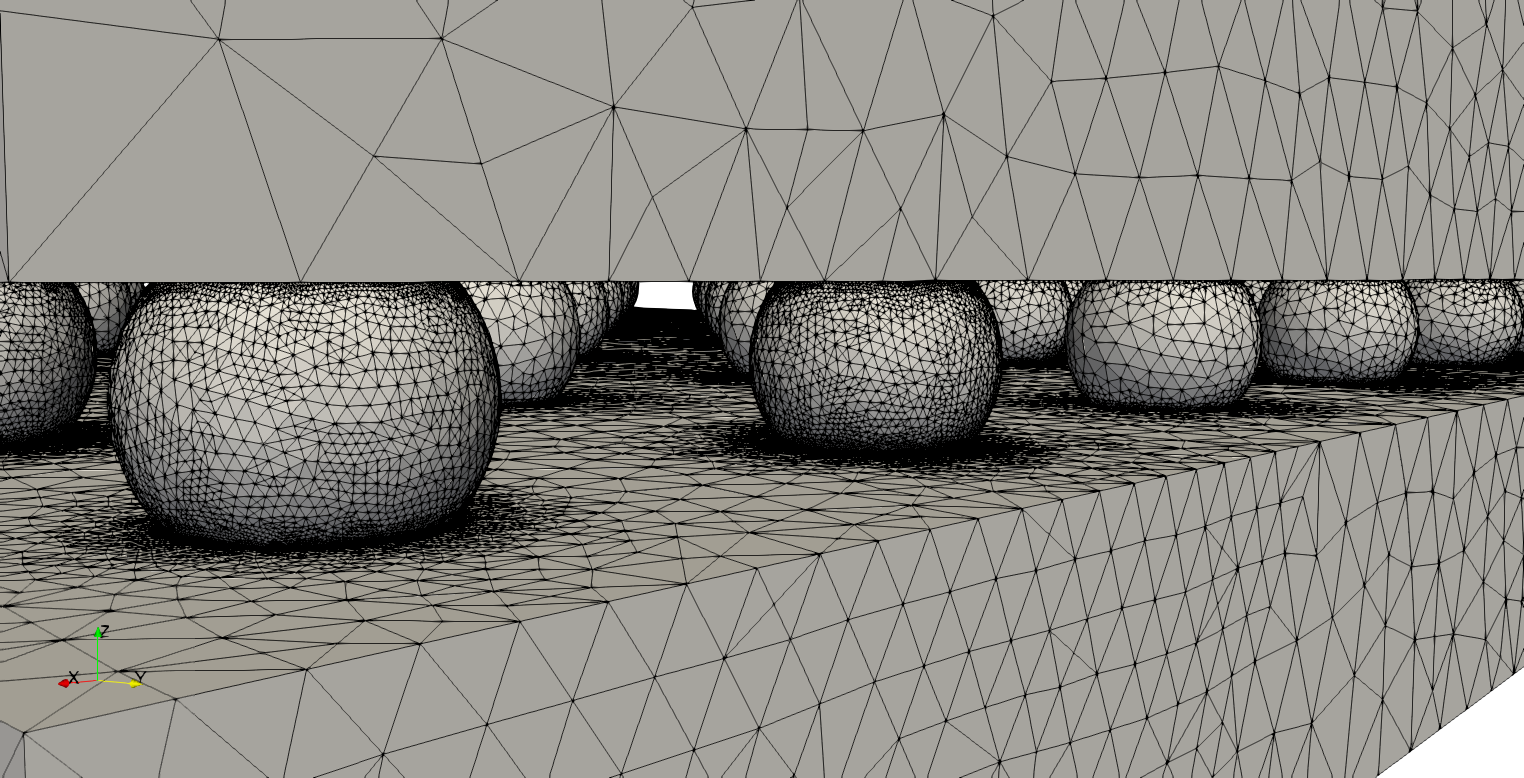
\includegraphics[width=.99\linewidth]{img/aut_solder_mesh_final2.png}
\end{subfigure}%
\caption{The initial mesh for the solder joint geometry (left) and the
final adapted mesh (right).}
\label{fig:aut_solder_mesh2}
\end{figure}

Figure \ref{fig:aut_solder_convergence} demonstrates the
convergence history of the error in the functional QoI,
as defined by the difference of the QoI obtained via
Richardson extrapolation and the QoI approximated by the
finite element solution. We compare the convergence for
two adaptive schemes, one achieved by successive uniform
refinements of the mesh and the other achieved by adjoint-based
error estimation. After 4 adaptive iterations, the adjoint-based
adaptive procedure achieves nearly the same degree of accuracy
as the uniform refinement procedure with two orders of
magnitude fewer degrees of freedom.

\begin{figure}[ht!]
\centering
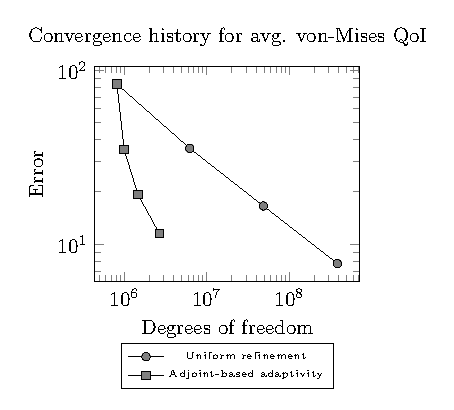
\includegraphics[width=0.5\linewidth]{img/aut_solder_convergence.pdf}
\caption{Error convergence histories for the solder joint example problem
with the average von-Mises stress QoI.}
\label{fig:aut_solder_convergence}
\end{figure}

Finally, we remark that automated parallel adaptive workflows
have been developed in reference \cite{bloomfield2017component}.
As an avenue for future investigation, adjoint-based error estimation
could be folded into these automated workflows.
In particular, an automated primal analysis could be used to inform
the actual selection of the QoI itself, which could then be accurately
assessed using adjoint-based error estimation.

%%% CONCLUSIONS
\section{Conclusions}

In this work, we have developed an automated approach for
adjoint-based error estimation and mesh adaptation for
execution on parallel machines. We have developed this approach
to be applicable to both Galerkin and stabilized finite
element methods. To realize this approach, we have extended
the concept of \emph{template-based generic programming} for
PDE models to include the automatic localization of error
contributions using a partition of unity-based
localization approach. We have demonstrated that this approach
is effective for a variety of example applications, including
nonlinear elasticity and elastoplasticity.

\chapter{IMAGE DRIVEN MACHINE LEARNING METHODS FOR MICROSTRUCTURE RECOGNITION}
\label{chap:COMMAT}

\let\thefootnote\relax\footnotetext{
This chapter previously appeared as:
A. Chowdhury, E. Kautz, B. Yener, and D. Lewis. "Image driven machine learning methods for microstructure recognition."  \emph{Computational Materials Science}, vol. 123 pp. 176-187, 2016.}



%%% INTRODUCTION
\section{Introduction}
\label{intro}

Materials characterization is a critical aspect of the material design and discovery process.  Recently, there has been much research in the field of materials informatics, a growing research area in which information technology and data science methods are used to interpret and analyze material data in order to accelerate the material discovery, design, and development process \cite{xu2015machine, Rodgers2006, Broderick2008, ferris2007materials, Kalidindi2011}.  Currently, material design relies on chance discoveries and follows a classical synthesis-characterization-theory-computation approach \cite{SergeiV.Kalinin2015}.  Further, there is a heavy reliance on individual researcher background and experience which introduces significant bias and potentially error into the process of microstructure recognition, interpretation, and characterization. 
%
For example, quantification of microstructures traditionally is done using stereological measurements.  Bias is introduced into stereological measurements through the requirement that an expert must first recognize and identify key microstructural features (inclusions, grains, or phases).  This bias can be caused by a variety of factors, such as an individual's background, education, and experiences \cite{SergeiV.Kalinin2015}.  

Although there have been recent advances in the field of quantitative microstructural science, there is still a heavy dependence on expert knowledge to identify what microstructural features are of interest for quantification \cite{DeCost2015}. Therefore it is desirable to expand upon work previously presented by DeCost and Holm in Reference \cite{DeCost2015}, and further explore methods of quantitative microstructure representations which do not require \textit{a priori} knowledge of microstructural features of interest or significance \cite{SergeiV.Kalinin2015}. This work aims to leverage existing computer vision and machine learning techniques specifically for the challenge of microstructure recognition.  While the overlap between computer vision, machine learning, and materials science is currently small \cite{SergeiV.Kalinin2015}, this work is a step towards increasing cross-disciplinary studies that challenge the current paradigm for microstructure characterization. 
%

Dendritic morphologies were chosen for this small case-study since dendrites are a well-characterized microstructural feature that exists in a variety of material systems (from single to multi-component).  Size, shape, and spacing of dendrites vary depending on solidification behavior and chemistry, thus micrographs of this single feature can vary widely.  The sample preparation and imaging methods used also contribute to the variety of micrographs produced from dendritic microstructures. Despite this variability in image data, it is still possible for human experts to look at a micrograph that contains dendrites and identify that it contains this microstructural feature, even though different orientations of dendrites (transverse or longitudinal) look distinctly different.  

Computer vision and machine learning methods were applied to the task of identifying a particular microstructural feature of interest (dendrites) from micrographs that do not contain this particular feature (just as a human expert would identify that a micrograph contains dendrites).  This recognition task is referred to in this work as Task 1.  Task 1 is a high-level microstructure recognition task in the sense that dendrites are a type of microstructural feature that are not specific to a material system.  A second classification task (referred to here as Task 2) was also completed, and involved distinguishing between longitudinal and transverse cross-sectional views of dendritic microstructures. This task may be viewed as a logical next step following the identification of dendrites in Task 1. If the micrograph from Task 1 was identified as a dendrite, then a second binary classification task was performed, with the goal of distinguishing between two different cross-sectional views.

The contribution in this work is to investigate multiple computer vision and machine learning methods for microstructure recognition. We hypothesize that the approach and methods presented here can be generalized, and thus applied to a variety of microstructure recognition tasks that act as a necessary first step in characterization of a material system.
%-----------------------------------------

\section{Alloy Fabrication and Sample Preparation}
\label{sample_prep}

The alloy fabrication, processing, and metallographic sample preparation procedure followed to obtain images used in this work was based on the process detailed in References \cite{Schaefer2005} and \cite{Mao2014} and is summarized here. 
%

A Materials Research Furnaces (MRF) three probe arc melter was used to fabricate alloys of varying Sn-Ag-Cu compositions.  After melting alloys were allowed to solidify and were then prepared for directional solidification (DS).  The solidified buttons were placed in a beaker on a hot plate.  The button was re-melted while constantly being purged with Ar gas to minimize sample oxidation. The alloy melt was then transferred into a 4 mm inner diameter quartz ampule with a mechanical pump.  The rods were allowed to cool, then removed from the ampule, and placed in a larger quartz ampule (5 mm inner diameter) for DS.  This ampule was then back-filled with Ar gas, sealed using a hydrogen torch, and inserted into the DS furnace.

DS was performed using a Bridgman-type apparatus in order to refine alloy microstructure.  The tube furnace in this apparatus is a Thermolyne Type-21100 fitted with an Omega temperature controller.
Following DS, alloys were removed from the quartz ampule, and small sections from the middle third of the rod were mounted in epoxy for metallographic sample preparation.  Sections were mounted such that transverse and longitudinal orientations of $\beta$-Sn dendrites could be viewed.  Samples were ground using silicon carbide (SiC) papers to 600 grit, then polished using 9, 3, and 1 $\mu$m diamond slurries.  Colloidal silica was used as the final polishing step and as a chemical etchant so that the dendritic microstructure would be readily visible using light optical microscopy.

%----------------------------------------------------------------------------------
\section{Image Data Sets}
\label{data_sets}

Image data used in this study includes micrographs taken over a span of approximately three years by students in the Lewis Research Group in the Materials Science and Engineering Department at Rensselaer Polytechnic Institute (RPI).  All images taken by Lewis Research Group members are of solder alloys with dendritic microstructures.  These alloys were manufactured, processed, and imaged at RPI, and a representative process of sample preparation was presented in Section \ref{sample_prep}.  In order to supplement micrographs obtained at RPI, micrographs from the publicly available Dissemination of Information Technology for the Promotion of Materials Science (DoITPoMS) library \cite{Barber2003} were used. Example images used in classification are provided in Figure \ref{fig:example_images}.   

Images were grouped into two data sets: Data Set 1 and Data Set 2, corresponding to classification Tasks 1 and 2 respectively. Data Set 1 is comprised of micrographs with and without dendritic morphologies.  This data set includes all images with dendrites (longitudinal and transverse cross-sections) from both the Lewis Group and the DoITPoMS micrograph library \cite{Barber2003}.  All micrographs that do not depict dendritic morphologies were obtained from the DoITPoMS library.  Data Set 1 includes 528 images that are each 227 by 227 square pixels. 264 original images were used in making Data Set 1 (132 micrographs containing dendrites and 132 micrographs without dendrites). Each original image is 270 by 500 pixels but includes a scale bar that interferes with feature extraction, therefore each image was cropped to yield two 227 by 227 square pixel images.  Thus, 528 images were used for classification. 

Data Set 2 is a subset of Data Set 1, and is comprised of micrographs that only contain dendrites, where each micrograph is either a transverse or longitudinal cross-sectional view.  Micrographs used in this data set include both images from the Lewis Group and the DoITPoMS micrograph library.  Data Set 2 contains a total of 188 images that are each 227 by 227 square pixels. As was done for Data Set 1, original images were cropped to remove the scale bar: 47 micrographs of each longitudinal and transverse sections (total of 94 original images) were cropped to create a 188 images used for classification.
%
\begin{figure}
  \begin{centering}
 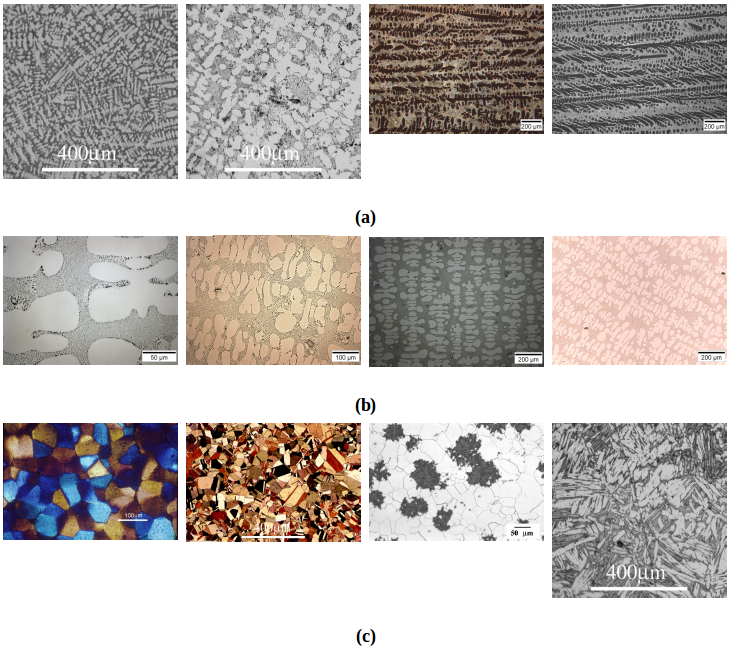
\includegraphics[scale=0.55]{img/example_images_v2.png}
 \caption{Examples of micrographs used in classification.  Micrographs shown in (a) and (b) are longitudinal and transverse cross-sectional views of dendrites, whereas micrographs in (c) do not contain dendrites.  Micrographs in (a), (b) and (c) were used in Task 1, and micrographs in (a) and (b) were used in Task 2.}
 \label{fig:example_images}
 \end{centering}
\end{figure}
%-----------------------------------------
\section{Approach}
\label{approach}
%
The general approach applied to the task of micrograph classification involved feature extraction and feature selection (dimensionality reduction) to compute feature vectors that were then used for training, validating, and testing various classification models.  The same approach was applied to both Data Sets 1 and 2 and is shown schematically in Figure \ref{fig:approach_overview}.

Feature extraction is the first step in the process of classifying micrographs.  Feature extraction starts with feature detection, where features in an image are local regions of pixels that include an `interesting' part of a microstructure, such as a corner, edge, or blob-like object. Features detected using computer vision algorithms are not necessarily semantically meaningful, however are pixel patterns that are mathematically repeatable and recognizable, thereby making the region a good feature. Detected features are then described (or represented) in the form of a vector, called a feature vector. A feature vector is comprised of a set of detected features in the image, and each image can thus be described or represented by a feature vector.  Multiple feature extraction methods were tested in this work in order to compare classification accuracies of different image representations.   
%

These feature vectors, derived in the process of feature extraction, have high dimensionality and in this work feature selection was performed after feature extraction for computational efficiency and to preclude the curse of dimensionality \footnote{The phrase `curse of dimensionality' refers to issues associated with increasing data dimensionality in Euclidean space.  Behavior of algorithms in low dimensional space, such as in three dimensions, may not generalize well to a higher dimensional space \cite{Keogh2010}.}.  Feature selection involves reducing the length of the feature vector while still retaining image information.  For example, if a feature vector is sparse, dimensionality reduction would involve reducing the sparsity of this vector.  Different dimensionality reduction methods were applied to test how each technique impacted classification accuracies.   

After feature extraction and selection, various classification models were trained, validated, and tested.  A 5 fold cross validation split was used for each data set.  This split was selected in order to minimize variance in model parameters%(determined via five-fold cross-validation on each of the 5 training folds), 
, and to avoid over-fitting.  These validation accuracies were then averaged and the standard deviation was calculated in order to evaluate model stability.  
%
\begin{figure}
  \begin{centering}
 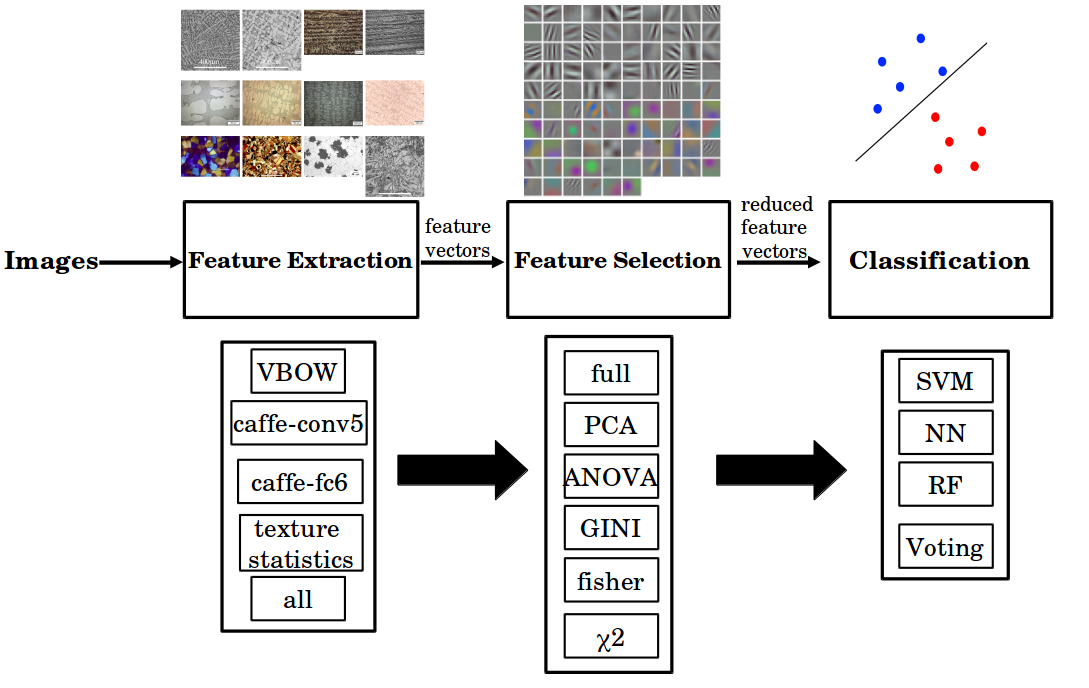
\includegraphics[scale=0.4]{img/flowchart_approach_updated.png}
 \caption{Overview of approach used in classification of micrograph data.  The approach summarized here shows 140 different combinations of feature extraction, feature selection and classification methods completed.  The same approach presented here was completed first for Task 1 (Data Set 1), then for Task 2 (Data Set 2).}
 \label{fig:approach_overview}
 \end{centering}
\end{figure}
%
We performed analysis on the two datasets (described in Section \ref{data_sets}) in the form of two classification tasks: Task 1 and Task 2. The relationship between these tasks is depicted in Figure \ref{fig:tasks_flowchart}. 

%Flowchart made using tikz
\begin{figure}
\centering

\begin{adjustbox}{width=\textwidth,height=0.75\textheight,keepaspectratio}
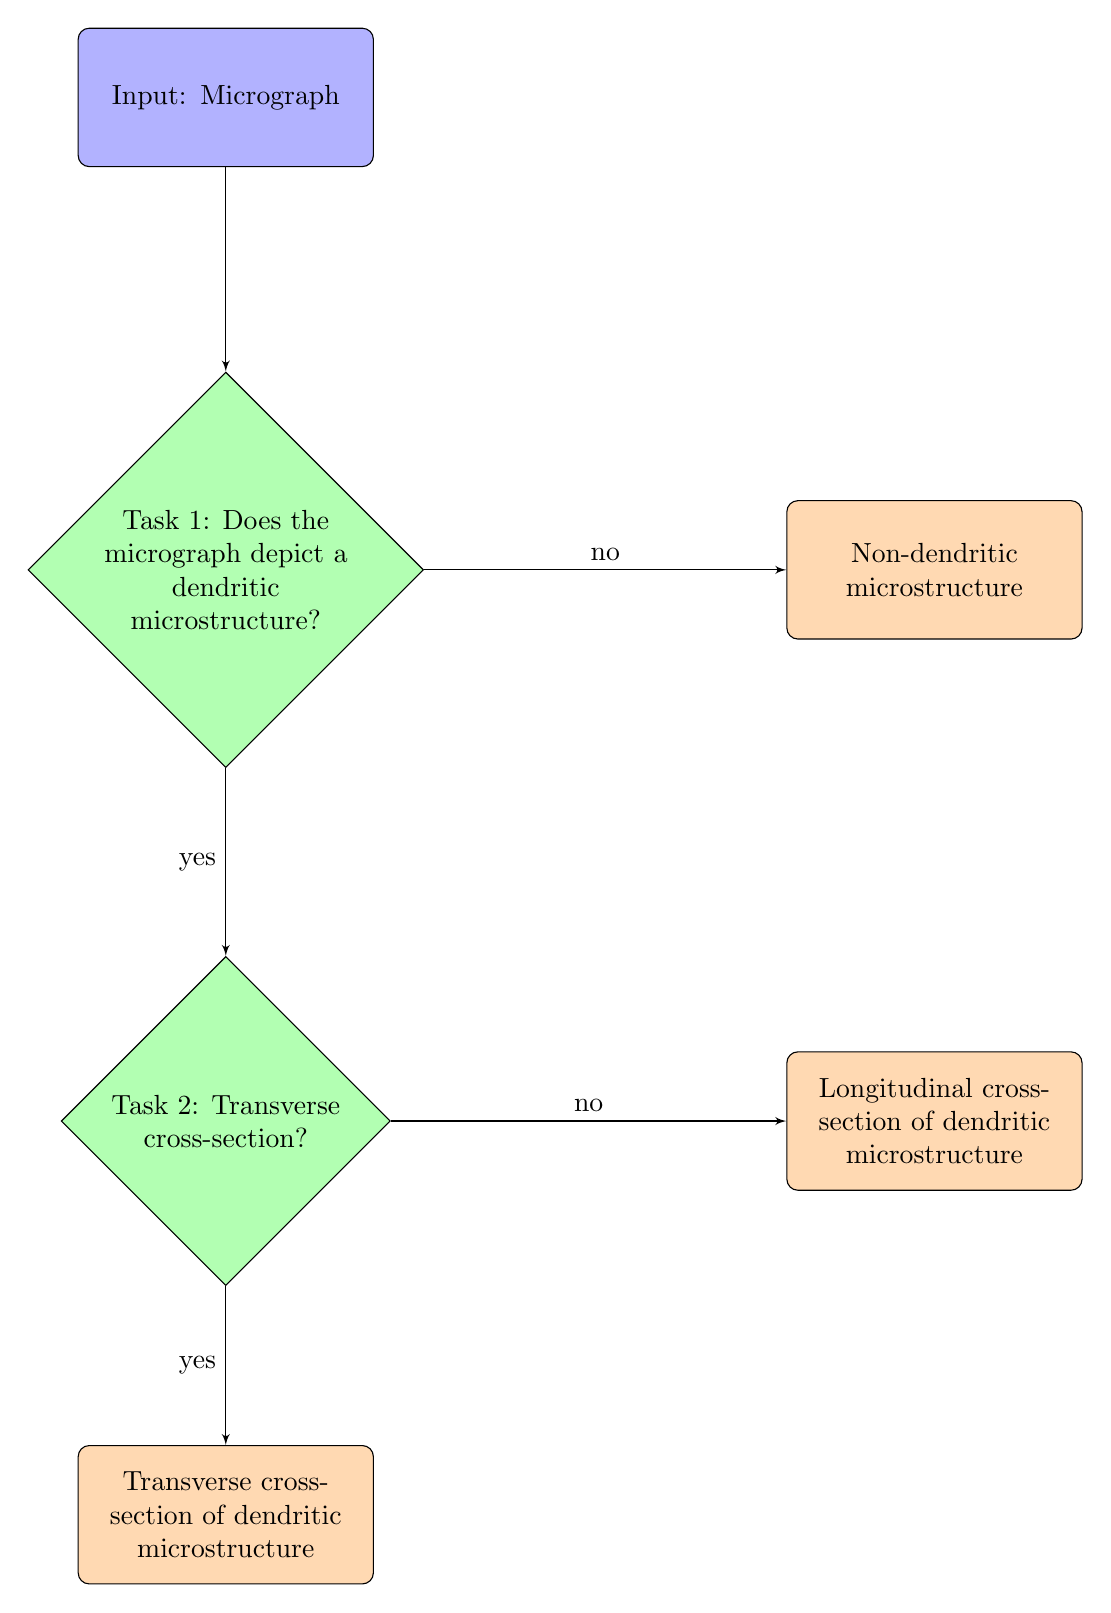
\begin{tikzpicture}
[node distance =  5cm]
    % Place nodes
    \node [input] (input) {Input: Micrograph};
    \node [decision, below of=input,yshift=-1cm] (task1) {Task 1: Does the micrograph depict a dendritic microstructure?};
    \node [decision, below of=task1,yshift=-2cm] (task2) {Task 2: Transverse cross-section?};
    \node [process, below of=task2,yshift=0cm] (trans) {Transverse cross-section of dendritic microstructure};
    
    \node [process, right of=task1, xshift=4cm] (nondendrite) {Non-dendritic microstructure};
    \node [process, right of=task2, xshift=4cm] (long) {Longitudinal cross-section of dendritic microstructure};
 
    % Draw edges
   \path [line] (input) -- (task1);
   \path [line] (task1) -- node [anchor=east] {yes} (task2);
   \path [line] (task2) -- node [anchor=east] {yes} (trans);
   \path [line] (task1) -- node [anchor=south]{no} (nondendrite);
   \path [line] (task2) -- node [anchor=south]{no} (long);

\end{tikzpicture}
\end{adjustbox}
\caption{Flowchart of microstructure recognition tasks, referred to here as Task 1 and Task 2.  Tasks 1 and 2 are both binary classification tasks.  Task 1 involves distinguishing between micrographs that depict dendritic morphologies from those that do not contain this particular microstructural feature.  From micrographs identified as containing dendrites (completed in Task 1), Task 2 involves distinguishing between different cross-sectional views (longitudinal or transverse) of dendritic microstructures.}
\label{fig:tasks_flowchart}
\end{figure}
%----------------------------------------------------------------------------------
\section{Computer Vision and Machine Learning Methods}
\label{methods}

As previously introduced in Section \ref{approach}, multiple feature extraction and selection methods were tested with various classifiers in order to evaluate the best methods to apply to microstructure recognition tasks.  The methods applied in this work are discussed in additional detail in Sections \ref{feature_extraction} - \ref{classification}.  Additionally, Section \ref{related_work} provides a brief overview of computer vision and machine learning methods applied to other research in the field of materials science. 

\subsection{Feature extraction}
\label{feature_extraction}

Feature extraction methods applied in this work are texture and shape statistics (which include Haralick texture features \cite{Haralick1973}, histogram of oriented gradients (HoG) \cite{Dalal2005}, local binary patterns (LBP) \cite{Ojala2002}, Hu moments \cite{Hu1962,Otsu1975}, Zernike Moments \cite{Khotanzad1990},threshold adjacency statistics \cite{Lievers2004}), visual bag of words (VBOW) \cite{Yang2007,Bay2006}, and pre-trained convolutional neural networks (CNN's).  We used the publicly available Caffe framework \cite{Jia2014} for all experiments involving pre-trained CNN's. The network was based on the architecture of Krizhevsky \textit{et al.} for ImageNet \cite{Krizhevsky2012}.  The approach of using a pre-trained network was taken in this case-study because this is a good first step that does not require training to determine model parameters, which would be a difficult task with the small data sets used in this study \cite{Jia2014}. 
  
Texture and shape statistics involve multiple feature extraction algorithms (previously listed) that operate on image texture and shape of objects within the image.  These methods are introduced below:   

Haralick features \cite{Haralick1973} are calculated using gray-level co-occurrence matrices (\textit{G$_{ij}$}, shown below) which are square matrices of size \textit{N$_g$} x \textit{N$_g$}, where \textit{N$_g$} is the number of gray levels in an image:
\\
\begin{equation}
%\[
G_{ij}=
  \begin{bmatrix}
    p(1,1) & p(1,2) & \cdots       & p(1,N_{g}) \\
    p(2,1) & p(2,2) &  \cdots      & p(2,N_{g}) \\
     \vdots &  \vdots &  \ddots    &  \vdots          \\
    p(N_{g},1)  & p(N_{g},2) & \cdots & p(N_{g},N_{g}) 
  \end{bmatrix}
%\]
\end{equation}
\\
Each matrix element, $ \ [i,j]\ $, is calculated by counting the number of times a pixel with value \textit{i} is adjacent to pixel with value \textit{j}.  When considering a square pixel image, there are four directions for which a gray-level co-occurrence matrix can be calculated: horizontal, vertical, left diagonal, and right diagonal.  Haralick texture statistics can be calculated based on the four gray-level co-occurrence matrices from each of these four directions. Haralick features thus describe the texture of an image. Fundamentally, texture is the arrangement of a certain feature or property, relative to the environment. In images, texture is the spatial distribution (arrangement) of gray-level variations in an image. Haralick features, computed from image gray-level co-occurrence matrices, capture texture patterns in an image. 

The histogram of oriented gradients (HoG) \cite{Dalal2005} method describes an image with a set of histograms of gradient orientations from local regions of an image (referred to as cells).  Each histogram reports the number of times a gradient orientation occurs in a given cell.  In general, an image gradient is a two-vector that points in the direction of the greatest rate of change.  The two components in the gradient vector include the gradient magnitude, $M(x,y)$, and the gradient orientation, $\alpha$$(x,y)$: 

\begin{equation}
%\[ M(x,y) = \sqrt{g_{x}^2+g_{y}^2} \]
M(x,y) = \sqrt{g_{x}^2+g_{y}^2}
\end{equation}
%\\
\begin{equation}
%\[ \alpha(x,y) = \tan^{-1}({\frac{g_{x}}{g_{y}}})\]
\alpha(x,y) = \tan^{-1}({\frac{g_{y}}{g_{x}}})
\end{equation}
\\
where $g_{x}$ and $g_{y}$ are the x and y components of the gradient respectively.  The normalized histograms of each cell are concatenated to form a descriptor vector for each image.  The greater the number of bins, the more detailed the histogram, and thus feature vector.

Local Binary Patterns (LBP) \cite{Ojala2002} method also describes the texture of an image.  Each image is split into cells and the neighborhood of each pixel (in each cell) is thresholded.  The neighborhood surrounding each pixel is defined by the pixel's eight nearest neighbors. When the center pixel intensity value is greater than its neighbor, the pixel value is changed to 0, otherwise the pixel value is 1. For each pixel, an 8-digit binary number, which can be referred to here as a label, is created. A histogram is created for each cell that reports the frequency of each label. The histograms for each cell are normalized, then all histograms are concatenated to yield a feature vector for the entire image. 

%A label is assigned by the operator to every pixel of an image by thresholding the neighborhood of each pixel with the center pixel value and using this result as a binary number. The local neighborhood is defined as a set of sampling points evenly spaced on a circle centered at the pixel to be labeled. Interpolation techniques are used when a sampling point does not fall on the center of the pixel.
%---------------------------------------------------------------------------------------------------------
Hu moments \cite{Hu1962,Otsu1975} are shape-based feature descriptors that describe, characterize, and quantify shapes of objects in an image.  
Hu moments are based on geometric moments, defined by $m_{p,q}(x,y)$: 

\begin{equation}
%\[ 
m_{p,q}(x,y) = \int_{-\infty}^{\infty} \int_{-\infty}^{\infty} x^{p} y^{q}f(x,y) dxdy
%\]
\end{equation}
\\
Since images are a collection of pixels, the moment of an image must be expressed in terms of summations instead of integrals, as follows: 
\begin{equation}
%\[ 
m_{p,q}(x,y) = \sum_{-\infty}^{\infty} \sum_{-\infty}^{\infty} x^{p} y^{q}f(x,y) dxdy
%\]
\end{equation}
\\

From the above equation, the area of an image would simply be defined by the 0th moment.  The centroid of an image can also be defined using this concept of geometric moments, as follows: 
\begin{equation}
%\[ 
(\bar{x},\bar{y}) = (\frac{m_{10}}{m_{00}} , \frac{m_{01}}{m_{00}})  
%\]
\end{equation}
\\
When moments are taken with respect to an image centroid, the moments are translation invariant, therefore a geometric moment can be defined relative to the centroid by $\mu_{p,q}(x,y)$:  
\begin{equation}
%\[ 
\mu_{p,q}(x,y) = \sum_{-\infty}^{\infty} \sum_{-\infty}^{\infty} (x-\bar{x})^{p}(y-\bar{y})^{q}f(x,y)dxdy 
%\]
\end{equation}
Hu derived seven moment invariants from the geometric moment equation, $\mu_{p,q}(x,y)$, that are invariant to scale, translation, and in-plane rotation and can be computed from a binary image. 
\\

In order to compute Hu moments, a binary image must be used.  A binary image was generated from the gray scale input images, by thresholding each image using Otsu's adaptive threshold algorithm \cite{Otsu1975}, which is a global thresholding method that selects the optimal threshold value based on the image histogram. Otsu's algorithm assumes the gray scale intensities of an image follow a bi-modal distribution with two classes, and the threshold value is selected to maximize the inter-class variance. Hu moments were computed based on connected components of pixels in the binary image.   \\

%-----------------------------------------
Zernike moments \cite{Khotanzad1990} are similar to Hu moments in that they describe the shape of objects in an image.  An important difference between Hu and Zernike moments is that Zernike polynomials are orthogonal basis functions for Zernike moments.  The use of orthogonal polynomials makes Zernike moments rotation invariant, and more robust to noise and minor variations in shape than Hu moments. Zernike moments are also calculated from a thresholded (binary) image.

%-----------------------------------------
Threshold adjacency statistics \cite{Lievers2004} are calculated from thresholded binary images. Three different binary images are generated from the original, using three different threshold values.  For each white pixel in an image, the number of neighboring white pixels is counted \cite{Klinger2012}.  The first statistic is the number of white pixels with no white neighbors.  The second statistic is the number of white pixels with one white neighbor.  The number of white pixels with white pixel neighbors up to eight is counted (where there are eight nearest neighbor for each pixel in an image).  Such statistics can be combined to create a feature vector that is subsequently used to distinguish and classify images.   

All texture and shape statistics used in feature extraction (Haralick texture features, HoG, LBP, Hu and Zernike moments, and threshold adjacency statistics) were used to create a 1,775 dimensional feature vector for each image that represents texture and shape of objects within the image. 

In addition to texture and shape statistics, Visual Bag of Words (VBOW) \cite{Yang2007,Bay2006} was also used for feature extraction. 
The VBOW technqiue is inspired from the  `bag of words' method used in document classification, where documents are considered as unordered sets of words. The corresponding words in the domain of image processing are local image features. These word descriptors are constructed around key points located by the Speeded Up Robust Features (SURF) \cite{Bay2006} key points detection algorithm.  These key points are extracted at regular locations at different scales making them very robust. The key point descriptors are categorized using a vector quantization technique such as $k$-means. The output of this discretization is a dictionary. Each image can therefore be encoded in the form of a histogram. This is done by extracting feature descriptors from the image, followed by finding the corresponding words to which the key points correspond to in the dictionary. The VBOW representation produced a 100-dimensional feature vector which was the pre-selected vocabulary size of the model.

A pre-trained convolutional neural network (CNN) model (trained on the Imagenet database) was also used in feature extraction. The ImageNet database contains 1.2 million images with 1000 categories. Here, the fifth and sixth layers of the pre-trained neural network were extracted and then used as feature descriptors for micrographs.
The sizes of the feature representation obtained from the pre-trained ImageNet model were 43,264 and 4,096 for the fifth layer (caffe-conv5) and sixth layer (caffe-fc6) respectively.  

Thus, for each image a feature vector was computed using each method described above. Concatenation of all computed feature vectors yielded a single vector which is referred to as \textgravedbl all\textacutedbl \ in Section \ref{results}.  Feature selection (dimensionality reduction) and classification was then performed using feature vectors from each method and the combined (concatenated) feature vector.     

\subsection{Dimensionality reduction}
\label{dimensionality_reduction}

Most of the image descriptors obtained from feature extraction methods lie in a high dimensional space (e.g. 1 x 43,264 for caffe-conv5).  Therefore it becomes necessary to employ dimensionality reduction techniques to bypass the curse of dimensionality \cite{curse}, and to improve computational efficiency.  The process of reducing feature vector dimensionality is called dimensionality reduction, or feature selection. Six different dimensionality reduction techniques were tested in this work: principle component analysis (PCA) \cite{pca}, ANOVA $F$-statistic (ANOVA) \cite{anova}, ${\chi}^2$ method \cite{chi}, Fisher score \cite{fisher}, and Gini index \cite{gini}. A brief description of each method is provided in this section. 

Principle component analysis (PCA)\cite{pca} is a feature transformation technique that uses orthogonal transformation to convert a set of observations of correlated variables to linearly uncorrelated ones. These orthogonal components are called principal components. In our work, we use only those principal components which account for 95 \% of the variance in the data. PCA can be thought of as a transformation that reveals the structure of the data in a way that best explains the variance in the data. The drawback of this technique is that the features obtained after reduction are linear combinations of the original feature variables which occupy a different vector space than the original variables. 

In addition to PCA, the Analysis of Variance (ANOVA) $F$-statistic \cite{anova} was used in feature selection. A one-way ANOVA F-test tests whether or not the different classes of the response variable have the same mean as the predictor variables. The $p$-value is calculated based on the $F$-statistic. These scores are then sorted in descending order and the features corresponding to the 30\textsuperscript{th} percentile are selected for analysis.

The ${\chi}^2$ test is used in statistics to test the independence of two events. In the domain of feature selection, it is used to test whether the occurrence of a particular variable and class are independent. The ${\chi}^2$ scores are ranked and the scores corresponding highest scores within the 30\textsuperscript{th} percentile are selected.

The idea behind the Fisher score is to find a subset of features such that the distance between data points in different classes is as large as possible and the distance between data instances in the same class are as small as possible. We select the features that correspond to the 30\textsuperscript{th} percentile of the highest Fisher scores.

%The idea behind the Minimum Redundancy Maximum Relevance (mrMR) \cite{mrmr} method was originally proposed by Pang et al. who proposed a feature selection technique that uses the mutual information criterion to score features. The key concept in  this feature selection procedure is to penalize a feature's relevancy by its redundancy in the presence of other selected features. The relevance of a feature subset is defined as the average value of the mutual information values between each individual feature and a particular class, whereas redundancy is the average of all the mutual information values between features. The mrMR criterion is therefore a combination of these two criteria (relevance and redundancy), which is defined as an optimization problem. The corresponding features which maximize the mrMR criterion are selected in this algorithm.

The Gini index \cite{gini} is an impurity splitting method, where impurity is calculated based on the probability that any sample belongs to a particular class. The minimum value of the index is 0, indicating that all of the members of the set belong to the same class, allowing for maximum useful information to be obtained. The opposite is true of samples in the set that are equally distributed in each class. The 30\textsuperscript{th} percentile threshold is used for selecting the features corresponding to Gini index scores.

\subsection{Classification}
\label{classification}

Classification was performed on Data Sets 1 and 2 using four different methods: support vector machine (SVM) \cite{svm}, random forest (RF)  \cite{rf}, nearest neighbor (NN)  \cite{nn}, and voting  \cite{voting}. SVM, NN, and Naive Bayes \cite{nb} models were used as components of the voting classifier.  Multiple classification algorithms were tested in order to determine which is the most accurate for micrograph classification. The classifiers applied to this case study were selected as representative models that have proven to yield high classification accuracies in other application areas, such as email filtering, text classification and more \cite{Kotsiantis2007}.  

Support vector machines (SVMs) \cite{svm} are discriminative (or margin based) classifiers. A SVM constructs a hyperplane in high dimensional space that may be used for classification. The hyperplane is selected such that the distance from it to the nearest data point on each side is maximized, referred to as the maximum margin hyperplane. We perform both linear and non-linear classification. We perform linear SVM classification on the original feature space and the non-linearity is introduced by the radial basis function (RBF) kernel for transforming data points to an infinite dimensional space. Our approach is to experiment with different learning algorithms. Therefore, we choose a representative algorithm from particular families of learning algorithms. The RBF kernel has proven to be a good representation for non-linear kernels. Linear SVM is referred to here as SVM-L, and non-linear SVM using a RBF is referred to as SVM-RBF.   

In addition to SVMs, nearest neighbor (NN) \cite{nn} classifier (an instance based classifier) was tested. The NN classifier assigns a test instance to a class based on the majority vote among the classes of the k-nearest neighbors of the training instances to the test instance. In our analysis, we selected k using five-fold cross validation. 

Random Forest (RF) classifiers \cite{rf}, also used in this work, are comprised of multiple decision trees and are therefore ensemble-based classifiers. A decision tree is a classification model that consists of a series of questions about the attributes of a data set, answers (such as yes or no), and follow-up questions. This series of questions is organized in a hierarchical manner and consists of edges that are connected to different types of nodes, including a root node, internal nodes, and leaf nodes. A root node has no incoming edges and zero or more outgoing edges.  An internal node has one incoming edge and two or more outgoing edges. A leaf node (also referred to as a terminal node) has one incoming edge and no outgoing edges. Each leaf node is assigned a label, and all internal and root nodes are assigned test conditions.  In order to perform classification using a decision tree model, a path is followed from root to terminal nodes.  This process will involve applying different test conditions, obtaining an answer, and moving to another internal node, and repeating this general process until a leaf/terminal node is reached.  The path followed in a decision tree model will yield a class label for a given data instance. Classification using RF is dependent on the prediction of class label from multiple decision trees. Each tree in the model gives a class label, and the RF chooses the class with the most votes among the decision trees. 
%-----------------------------------------
Similar to RF, the voting classifier \cite{voting} is also an ensemble-based classifier that is based on majority voting among various classification modules. With RF, the modules were decision trees, and in this work we perform voting among three independent algorithms: SVM-RBF, NN and Naive Bayes. \\

Naive Bayes is a classifier model that depends on the inherent distribution of the training data set, and is thus categorized as a generative classifier.  The Naive Bayes classifier uses Bayes' probability model and a decision rule to predict class of a data instance, where in this work each data instance is an image.    

%probability
Naive Bayes is a statistical classifier that uses the concept of posterior probability for classification of new data instances.  Each new data instance is assigned the class label that has the highest posterior probability. For a given set of variables $X={x_{1}, x_{2}...x_{d}}$, the posterior probability for event $C_{j}$ is calculated from the set of possible outcomes, $C={c_{1}, c_{2}, ... c_{d}}$, where the set of possible outcomes is all class labels. Bayes' rule defines posterior probability of a class label (the probability $X$ belongs to $C_{j}$) as:
%Bayes Rule 
\begin{equation}
p(C_{j}|x_{1}, x_{2}, ... x_{d}) \propto p(x_{1}, x_{2}, ...x_{d} | C_{j})p(C_{j})
\end{equation}

where $p(C_{j}|x_{1}, x_{2}, ... x_{d})$ is the posterior probability of class label $C_{j}$. Posterior probability can be re-written, given that conditional probabilities of independent variables are assumed to be statistically independent: 

\begin{equation}
p(C_{j}|X) \propto \prod_{k=1}^{d} p(C_{j}) p(x_{k}|C_{j})
\end{equation}

Using the Naive Bayes classifier, the new data instance $X$ is classified by the class label $C_{j}$ that has the highest posterior probability. In addition to the probability model defined above, the maximum \textit{a posteriori} decision rule is applied for classification, meaning the hypothesis that is most probable is selected as the class label.
%-----------------------------------------

Classification was completed using each of the methods detailed above, for the full data set in addition to the reduced data sets obtained by the different feature selection techniques detailed in Section \ref{dimensionality_reduction}.  Model parameters were determined using five-fold cross-validation.  

In order to determine model accuracy and stability, average classification accuracies and standard deviations were calculated for every possible combination of classification, feature extraction, and feature selection method used.  Average classification accuracies were calculated by taking the average of 5 fold cross validation of the dataset. The parameters of each algorithm were selected using the training fold of each split. Therefore the parameters were selected using another 5 fold cross validation of the training set and the training set was re-trained using the best combination of the parameters and the test accuracy on the remaining validation fold was calculated. This was performed 5 times and the average and standard deviation of the 5-fold validation accuracies was calculated.
%---------------------------------------------------------------------------------
%Methods that have been applied in the field of materials science and engineering....

\subsection{Related Work in Materials Science}
\label{related_work}

The methods discussed here are well established in the computer vision and machine learning disciplines, however only a select few have been previously applied to materials science and engineering challenges.  Shape descriptor methods, such as Hu moment invariants, have previously been used to quantitatively describe microstructures for subsequent classification \cite{Pattan2010, Prakash2011, Kumara,MacSleyne2008,Sluytman2012}.  
%
Specific applications of Hu moments in the field of materials science include automated classification of precipitate shapes in a two-phase microstructure \cite{MacSleyne2008}, classification of cast iron microstructures \cite{Pattan2010,Prakash2011,Kumara}, and analysis of precipitate shapes in nickel-based superalloys \cite{Sluytman2012}.\\

%
Additionally, the Visual Bag of Words feature extraction method with a Support Vector Machine classifier were used for multi-class classification of microstructures by DeCost and Holm \cite{DeCost2015}, as previously mentioned in Section \ref{intro}. 

%----------------------------------------------------------------------------------------------------------------------------
\section{Selection of Model Parameters}
Each algorithm involved in our experimentation has their own set of parameters. Some of the parameters are set \textit{a priori} and some are tuned using 5-fold cross-validation. Since we used cross validation to set the parameters for each combination of feature extraction, feature selection and classifier, there is no specific setting for each individual parameter for the algorithm. This approach of using 5-fold cross-validation to set parameters generates results that are more robust and thus more accurate with respect to each particular combination of feature extraction, feature selection, and classifier. We do a grid search over the parameter space using 5-fold cross-validation to estimate the best setting of the different parameters. Such parameters include number of neighbors in the nearest neighbor classifier, the SVM margin parameter ($C$), the RBF kernel parameter  ($\gamma$), the number of trees or estimators in the random forests classifier. The parameters found by cross-validation are presented in detail in the supplementary article to this paper.

We also set a number of parameters before the experiments are run to limit the number of parameters to tune using cross-validation. Such set parameters include the those listed in Table \ref{tab:parameters}. 

%The Hessian threshold for the SURF detector was set to 500. The dictionary size for Visual Bag of Words was set to 100. The radius of the local binary patterns was set to 5 and the number of points to 10. The radius for Zernike moments was set to 5. 

%\begin{table}[H]
%\centering
%%\renewcommand{\arraystretch}{1}
%\captionsetup{justification=centering}
%\caption{Feature extraction parameters selected for use in experimentation.}
%\label{tab:parameters}
%%\resizebox{\linewidth}{!}{
%\begin{tabular}{|c|c|} \hline
%
%\textbf{Parameter}	&	\textbf{Value}	\\	\hline
%Hessian threshold for SURF detector & 500 \\ \hline
%Dictionary size for VBOW & 100 \\ \hline
%Radius of LBP & 5\\ \hline
%Number of points in LBP & 10 \\ \hline 
%Radius for Zernike moments & 5 \\ \hine
%\hline
%\end{tabular}
%%}
%\end{table}


Default values were used for other parameters. We set the parameters in the feature extraction algorithms because this would represent a consistent test bed for the thorough computational experimentation over the feature selection and classification algorithms.

\section{Software and Hardware Specifications}
All of our experimentation was carried out with Python version 2.7 with the help  of various open-source libraries. The opencv, scipy, skimage, numpy, mahotas and caffe packages (compatible with the Python version used in this work) were used for feature extraction. The skfeature library was used for experimentation with the various feature selection algorithms. The sklearn package was used for the various learning algorithms.

The hardware used for experimentation was a 3.3 GHz 4 core Intel i5 CPU.
%----------------------------------------------------------------------------------
\section{Results and Discussion}
\label{results}

This section reports the results from applying multiple feature extraction, feature selection, and classification methods to the task of micrograph recognition.    
%
Performance comparisons between feature extraction, selection, and classification methods are presented in Sections \ref{Task1} and \ref{Task2}.  The success of different methods are compared based on the mean classification accuracies and standard deviations.
%
Results are presented in the form of tables, where each table compares all possible combinations of the three modalities (i.e. feature extraction, feature selection, and classification) that yield the maximum classification accuracy.  The tables presented here summarize a large set of results that are provided in a supplement to this article. 

%--------------------------------------------------------------
\subsection{Task 1 - Dendritic versus non-dendritic microstructures}
\label{Task1}

Table \ref{tab:FE_Task1} reports the feature extraction methods that yielded maximum classification accuracies for each combination of feature selection and classifier tested.  It is clear from Table \ref{tab:FE_Task1} that caffe-fc6 was the most effective feature extraction method because the majority of the maximum classification accuracies in Table \ref{tab:FE_Task1} were computed using feature vectors obtained using caffe-fc6.  These results suggest that microstructure image data is represented well using pre-trained neural networks (a type of deep learning algorithm), and this feature extraction method generalizes well.  

It is also important to note that caffe-fc6 was not re-trained on Data Sets 1 and 2 used in this case study.  The pre-trained weights determined via training on the millions of natural images in the ImageNet database were used, which were successfully applied to feature extraction here.  This result is significant because in using a pre-trained neural network, no large database (i.e. millions) of micrographs was needed.  The use of the sixth  layer (fully connected) from the Caffe network \cite{Jia2014} for feature extraction (caffe-fc6) resulted in superior classification performance over other feature extraction methods such as VBOW and texture and shape statistics for Task 1. 

It is suggested that caffe-fc6 produced higher classification accuracies overall than VBOW and texture and shape statistics for Task 1 based on the difference in image representations (in the form of feature vectors) between each method.  
%
Furthermore, caffe-fc6 provided a more accurate image representation than caffe-conv5 (the 5th convolution layer of the Caffe network).  This result could be due to the fact that features extracted from the sixth layer  was more representative of the image dataset. 

%--------------------------------------------------
%updated 06/10/16
\begin{table}[H]
\centering
\renewcommand{\arraystretch}{1}
\captionsetup{justification=centering}
\caption{Feature extraction methods and corresponding classification accuracies (in \%), that contributed to the maximum classification accuracy for each combination of feature selection and classification method tested for Task 1.}
\label{tab:FE_Task1}
\resizebox{\linewidth}{!}{
\begin{tabular}{|c|c|c|c|c|c|} \hline
	 & 	\multicolumn{5}{|c|}{\textbf{Classifier}} 									\\	\hline
\textbf{Feature }	&		&		&		&		&		\\	
\textbf{Selection}	&	\textbf{SVM-L}	&	\textbf{SVM-RBF}	&	\textbf{NN}	&	\textbf{RF}	&	\textbf{Voting}	\\	\hline
\multirow{2}{*}{\textbf{Full}}	&	\textbf{caffe-fc6}	&	\textbf{caffe-fc6}	&	\textbf{caffe-fc6}	&	\textbf{caffe-fc6}	&	\textbf{caffe-fc6}	\\	
	&	90.52 $\pm$ 4.9	&	90.52 $\pm$ 4.9	&	 87.69 $\pm$ 4.69	&	87.88 $\pm$ 6.19	&	89.02 $\pm$ 5.54	\\	\hline
\multirow{2}{*}{\textbf{PCA}}	&	\textbf{caffe-fc6}	&	\textbf{caffe-fc6}	&	\textbf{caffe-fc6}	&	VBOW 	&	\textbf{caffe-fc6}	\\	
	&	89.03 $\pm$ 3.58	&	89.03 $\pm$ 3.58	&	89.96 $\pm$ 2.53	&	87.88 $\pm$ 1.84	&	88.64 $\pm$ 3.09	\\	\hline
\multirow{2}{*}{\textbf{ANOVA}}	&	\textbf{caffe-fc6}	&	\textbf{caffe-fc6}	&	\textbf{caffe-fc6}	&	\textbf{caffe-fc6}	&	\textbf{caffe-fc6}	\\	
	&	90.91 $\pm$ 4.32	&	90.91 $\pm$ 4.32	&	87.31 $\pm$ 3.23	&	87.13 $\pm$ 5.35	&	91.85 $\pm$ 4.25	\\	\hline
\multirow{2}{*}{$\mathbf{{\chi}^2}$}	&	\textbf{caffe-fc6}	&	\textbf{caffe-fc6}	&	\textbf{caffe-fc6}	&	caffe-conv5 	&	\textbf{caffe-fc6}	\\	
	&	90.54 $\pm$ 3.99	&	 90.54 $\pm$ 3.99	&	87.3 $\pm$ 3.73	&	87.49 $\pm$ 4.5	&	90.53 $\pm$ 4.96	\\	\hline
\multirow{2}{*}{\textbf{fisher}}	&	\textbf{caffe-fc6}	&	\textbf{caffe-fc6}	&	\textbf{caffe-fc6}	&	texture-statistics 	&	texture-statistics 	\\	
	&	89.01 $\pm$ 5.82	&	 89.01 $\pm$ 5.82	&	89.58 $\pm$ 5	&	87.5 $\pm$ 6.1	&	89.58 $\pm$ 5.76	\\	\hline
\multirow{2}{*}{\textbf{GINI}}	&	texture-statistics 	&	texture-statistics 	&	\textbf{caffe-fc6}	&	texture-statistics 	&	caffe-conv5 	\\	
	&	89.01 $\pm$ 4.05	&	89.01 $\pm$ 4.05	&	89.39 $\pm$ 4.64	&	87.5 $\pm$ 5.46	&	89.58 $\pm$ 6.32	\\	\hline

\end{tabular}}
\end{table}
%----------------------------------------------------------------------------------

Feature selection was also investigated in order to determine if there was an overall best method for dimensionality reduction, and results are provided in Table \ref{tab:FS_Task1}.  From results presented here, there is no one feature selection method that provided maximum classification accuracies for the majority of feature extraction and classifier combinations tested.  This result could be attributed to the variability in the micrographs that do not depict dendrites (in Data Set 1).  The micrographs selected as depicting non-dendritic morphologies are not all from the same material system and there is no common microstructural feature amongst this class. 

The results also show that the feature selection method is sensitive to the types of feature extraction techniques and classifier models applied. Therefore, choice of dimensionality reduction should depend on the methods used for classification and feature extraction.

	
%-----------------------------------------------------------------------
%updated 06/09/16 - no mrmr in this table, no changes needed
\begin{table}[H]
\centering
\renewcommand{\arraystretch}{1}
\captionsetup{justification=centering}
\caption{Feature selection methods and corresponding classification accuracies (in \%), that contributed to the maximum classification accuracy for each combination of feature extraction and classification method tested for Task 1.}
\label{tab:FS_Task1}
\resizebox{\linewidth}{!}{
\begin{tabular}{|c|c|c|c|c|c|} \hline

	&	\multicolumn{5}{|c|}{\textbf{Classifier}} 									\\	\hline
\textbf{Feature }	&		&		&		&		&		\\	
\textbf{Extraction}	&	\textbf{SVM-L}	&	\textbf{SVM-RBF}	&	\textbf{NN}	&	\textbf{RF}	&	\textbf{Voting}	\\	\hline
\multirow{2}{*}{\textbf{VBOW}}	&	Full 	&	Full	&	Full	&	PCA	&	Full 	\\	
	&	86.93 $\pm$ 2.09	&	 86.93 $\pm$ 2.09	&	 84.45 $\pm$ 3.16	&	 87.88 $\pm$ 1.84	&	85.4 $\pm$ 3.53	\\	\hline
\multirow{2}{*}{\textbf{caffe-fc6}}	&	ANOVA 	&	ANOVA	&	PCA	&	Full	&	ANOVA	\\	
	&	90.91 $\pm$ 4.32	&	 90.91 $\pm$ 4.32	&	 89.96 $\pm$ 2.53	&	 87.88 $\pm$ 6.19	&	91.85 $\pm$ 4.25	\\	\hline
\multirow{2}{*}{\textbf{caffe-conv5}}	&	ANOVA 	&	ANOVA	&	ANOVA	&	${\chi}^2$	&	${\chi}^2$	\\	
	&	89.96 $\pm$ 6.11	&	89.96 $\pm$ 6.11	&	 85.04 $\pm$ 4.48	&	 87.49 $\pm$ 4.5	&	90.15 $\pm$ 5.08	\\	\hline
\multirow{2}{*}{\textbf{texture-statistics}}	&	${\chi}^2$	&	${\chi}^2$	&	fisher	&	fisher	&	${\chi}^2$	\\	
	&	 89.96 $\pm$ 5.37	&	89.96 $\pm$ 5.37	&	 89 $\pm$ 5.74	&	 87.5 $\pm$ 6.1	&	89.78 $\pm$ 4.82	\\	\hline
\multirow{2}{*}{\textbf{combined}}	&	${\chi}^2$	&	${\chi}^2$	&	fisher	&	GINI	&	${\chi}^2$	\\	
	&	89.96 $\pm$ 5.37	&	89.96 $\pm$ 5.37	&	 89 $\pm$ 5.74	&	86.74 $\pm$ 5.51	&	89.78 $\pm$ 4.8	\\	\hline

\end{tabular}}
\end{table}

%--------------------------------------------------------------------------------

Performance comparisons of classification models were also done for Task 1, and results are provided in Table \ref{tab:Classifier_Task1}.  Linear SVM (SVM-L) provides maximum classification accuracies for over 50\% of the possible feature extraction and selection combinations, indicating that this model generalizes well.
%%ARITRA- DOES THIS MAKE SENSE?: 
This result also demonstrates that the data is linearly separable and use of a Gaussian kernel is not necessary for Task 1. 

%--------------------------------------------------------------
%updated 06/10/16
\begin{table}[H]
\centering
\renewcommand{\arraystretch}{1}
\captionsetup{justification=centering}
\caption{Classification methods that contributed to the maximum classification accuracy (in \%) for each combination of feature extraction and feature selection method tested for Task 1.}
\label{tab:Classifier_Task1}
\resizebox{\linewidth}{!}{
\begin{tabular}{|c|c|c|c|c|c|} \hline
	&	\multicolumn{5}{|c|}{\textbf{Feature Extraction}} 									\\	\hline
\textbf{Feature }	&		&		&		&		&		\\	
\textbf{Selection}	&	\textbf{VBOW}	&	\textbf{caffe-fc6}	&	\textbf{caffe-conv5}	&	\textbf{texture-statistics}	&	\textbf{combined}	\\	\hline
\multirow{2}{*}{\textbf{Full}}	&	\textbf{SVM-L}	&	\textbf{SVM-L}	&	RF 	&	\textbf{SVM-L}	&	\textbf{SVM-L}	\\	
	&	 86.93 $\pm$ 2.09	&	90.52 $\pm$ 4.9	&	87.12 $\pm$ 4.37	&	 87.88 $\pm$ 3.98	&	 87.88 $\pm$ 3.98	\\	\hline
\multirow{2}{*}{\textbf{PCA}}	&	RF 	&	NN 	&	\textbf{SVM-L}	&	\textbf{SVM-L}	&	\textbf{SVM-L}	\\	
	&	87.88 $\pm$ 1.84	&	89.96 $\pm$ 2.53	&	87.3 $\pm$ 4.43	&	 88.64 $\pm$ 3.32	&	88.64 $\pm$ 3.32	\\	\hline
\multirow{2}{*}{\textbf{ANOVA}}	&	RF 	&	Voting	&	\textbf{SVM-L}	&	\textbf{SVM-L}	&	\textbf{SVM-L}	\\	
	&	83.72  $\pm$ 1.99	&	 91.85  $\pm$ 4.25	&	89.96  $\pm$ 6.11	&	89.78  $\pm$ 5.76	&	89.78  $\pm$ 5.76	\\	\hline
\multirow{2}{*}{$\mathbf{{\chi}^2}$}	&	\textbf{SVM-L}	&	\textbf{SVM-L}	&	Voting	&	\textbf{SVM-L}	&	\textbf{SVM-L}	\\	
	&	80.29 $\pm$ 3.58	&	90.54 $\pm$ 3.99	&	 90.15 $\pm$ 5.08	&	89.96 $\pm$ 5.37	&	89.96 $\pm$ 5.37	\\	\hline
\multirow{2}{*}{\textbf{fisher}}	&	\textbf{SVM-L}	&	NN 	&	Voting 	&	Voting	&	Voting	\\	
	&	78.4 $\pm$ 1.64	&	89.58 $\pm$ 5	&	89.57 $\pm$ 6.5	&	 89.58 $\pm$ 5.76	&	 89.58 $\pm$ 5.76	\\	\hline
\multirow{2}{*}{\textbf{GINI}}	&	Voting	&	NN	&	Voting	&	\textbf{SVM-L}	&	\textbf{SVM-L}	\\	
	&	 77.82 $\pm$ 2.85	&	 89.39 $\pm$ 4.64	&	 89.58 $\pm$ 6.32	&	 89.01 $\pm$ 4.05	&	 89.01 $\pm$ 4.05	\\	\hline

\end{tabular}}
\end{table}

%--------------------------------------------------------------
\subsection{Task 2 - Longitudinal versus transverse cross-sectional views of dendrites} 
\label{Task2}
%--------------------------------------------------------------

Similar performance comparisons presented for Task 1 in Section \ref{Task1} were also completed for Task 2 (longitudinal vs. transverse cross-sectional views of dendrites).  A similar result was observed when feature extraction methods were evaluated, where caffe-fc6 represented micrographs well. 

Again, features extracted using pre-trained neural networks dominates Table \ref{tab:FE_Task2}. This result shows that the features extracted from the sixth, fully connected layer in the Caffe network (caffe-fc6) have meaningful and distinguishable characteristics in terms of microstructural images.  
%
Although the majority of the maximum classification accuracies used features extracted via caffe-fc6, even higher values for classification accuracy were obtained using texture statistics and caffe-conv5 with a a linear SVM classifier. Classification accuracies obtained via SVM-L varied based on the feature selection method used, however the overall classification accuracies were highest for this classifier with features computed from either texture statistics or caffe-conv5.  %These feature extraction methods, used in conjunction with various feature selection techniques and SVM-L could have resulted in higher classification accuracies due to.........
%
One major disadvantage of using texture statistics for feature extraction is that this method is a combination of multiple different feature detectors, and required prior knowledge of various techniques, that all perform differently depending on shape and texture of input data. 
%
The success of SVM as a classifier is subsequently discussed in additional detail.  

%---------------------------------------------------------------
%updated 06/10/16 - mrMR removed
\begin{table}[H]
\centering
\renewcommand{\arraystretch}{1}
\captionsetup{justification=centering}
\caption{Feature extraction methods and corresponding classification accuracies (in \%), that contributed to the maximum classification accuracy for each combination of feature selection and classification method tested for Task 2.}
\label{tab:FE_Task2}
\resizebox{\linewidth}{!}{
\begin{tabular}{|c|c|c|c|c|c|} \hline
	 & 	\multicolumn{5}{|c|}{\textbf{Classifier}} 									\\	\hline
\textbf{Feature }	&		&		&		&		&		\\	
\textbf{Selection}	&	\textbf{SVM-L}	&	\textbf{SVM-RBF}	&	\textbf{NN}	&	\textbf{RF}	&	\textbf{Voting}	\\	\hline
\multirow{2}{*}{\textbf{Full}}	&	texture-statistics 	&	\multirow{14}{*}{\textbf{caffe-fc6:} 95.74 $\pm$ 3.73}	&	\multirow{14}{*}{\textbf{caffe-fc6:} 94.49 $\pm$ 1.46}	&	\textbf{caffe-fc6} 	&	\multirow{14}{*}{\textbf{caffe-fc6:} 94.99 $\pm$ 2.38 }	\\	
	&	95.79 $\pm$ 3.94	&		&		&	87.88 $\pm$ 1.64	&		\\	
\multirow{2}{*}{\textbf{PCA}}	&	texture-statistics 	&		&		&	VBOW 	&		\\	
	&	96.84 $\pm$ 3.07	&		&		&	87.88 $\pm$ 2.95	&		\\	
\multirow{2}{*}{\textbf{ANOVA}}	&	texture-statistics 	&		&		&	\textbf{caffe-fc6} 	&		\\	
	&	97.37 $\pm$ 3.33	&		&		&	87.13 $\pm$ 1.64	&		\\	
\multirow{2}{*}{$\mathbf{{\chi}^2}$}	&	caffe-conv5 	&		&		&	caffe-conv5 	&		\\	
	&	96.78 $\pm$ 2.63	&		&		&	87.49 $\pm$ 15.69	&		\\	
\multirow{2}{*}{\textbf{fisher}}	&	caffe-conv5 	&		&		&	texture-statistics 	&		\\	
	&	97.84 $\pm$ 2.65	&		&		&	87.5 $\pm$ 8.25	&		\\	
\multirow{2}{*}{\textbf{GINI}}	&	caffe-conv5 	&		&		&	texture-statistics 	&		\\	
	&	97.31 $\pm$ 2.42	&		&		&	87.5 $\pm$ 8.25	&		\\	\hline

\end{tabular}}
\end{table}

%----------------------------------------------------------------------------------
Results from comparing feature extraction and classifier combinations indicate that in many cases feature selection did not improve calculated classification accuracies, as was seen in Task 1 results.  This is shown in Table \ref{tab:FS_Task2} by the majority of maximum classification accuracies computed using the full feature vector. 
%
When SVM-L was used for classification, feature selection methods improved results.  The feature selection method used with SVM-L that yielded the maximum classification accuracy depended on the feature representation obtained in the feature extraction step. 
%
The same classification accuracies were obtained for each feature selection method, for a given feature extraction and classifier combination. In addition, the features extracted from the fifth layer (convolutional) in the pre-trained neural network perform poorly with respect to the other extraction methodologies. This can be attributed to the fact that caffe-conv5 produces the feature representation with the highest dimensionality which is an order of magnitude greater than the second largest feature vector (caffe-fc6). Therefore, features extracted using caffe-conv5 are not robust (i.e. they have low accuracy with high standard deviation).  Being lower in the network hierarchy of the CNN also means that the features may not be tuned properly to the task, and therefore features provide a less accurate image representation than features computed via caffe-fc6.  
%----------------------------------------------------------------------------------
\begin{table}[H]
\centering
\renewcommand{\arraystretch}{1}
\captionsetup{justification=centering}
\caption{Feature selection methods, and corresponding classification accuracies (in \%), that contributed to the maximum classification accuracy for each combination of feature extraction and classification method tested for Task 2.}
\label{tab:FS_Task2}
\resizebox{\linewidth}{!}{
\begin{tabular}{|c|c|c|c|c|c|} \hline
	&	\multicolumn{4}{|c|}{\textbf{Classifier}} 							\\	\hline		
\textbf{Feature }	&		&		&		&		&		\\	
\textbf{Extraction}	&	\textbf{SVM-L}	&	\textbf{SVM-RBF}	&	\textbf{NN}	&	\textbf{RF}	&	\textbf{Voting}	\\	\hline
\multirow{2}{*}{\textbf{VBOW}}	&	ANOVA 	&	\textbf{Full}	&	\textbf{Full}	&	PCA 	&	\textbf{Full}	\\	
	&	96.32 $\pm$ 2.68	&	93.73 $\pm$ 3.96	&	 92.73 $\pm$ 3.91	&	87.88 $\pm$ 2.95	&	93.98 $\pm$ 3.09	\\	\hline
\multirow{2}{*}{\textbf{caffe-fc6}}	&	GINI 	&	\textbf{Full}	&	\textbf{Full}	&	\textbf{Full}	&	\textbf{Full}	\\	
	&	96.78 $\pm$ 2.63	&	95.74 $\pm$ 3.73	&	94.49 $\pm$ 1.46	&	87.88 $\pm$ 1.64	&	94.99 $\pm$ 2.38	\\	\hline
\multirow{2}{*}{\textbf{caffe-conv5}}	&	fisher 	&	\textbf{Full}	&	\textbf{Full}	&	${\chi}^2$	&	\textbf{Full}	\\	
	&	97.84 $\pm$ 2.65	&	84.46 $\pm$ 13.6	&	77.19 $\pm$ 14.62	&	 87.49 $\pm$ 15.69	&	78.45 $\pm$ 16.66	\\	\hline
\multirow{2}{*}{\textbf{texture-statistics}}	&	ANOVA 	&	\textbf{Full}	&	\textbf{Full}	&	fisher 	&	\textbf{Full}	\\	
	&	97.37 $\pm$ 3.33	&	93.23 $\pm$ 11.58	&	94.24 $\pm$ 5.03	&	87.5 $\pm$ 8.25	&	93.73 $\pm$ 11.09	\\	\hline
\multirow{2}{*}{\textbf{combined}}	&	ANOVA 	&	\textbf{Full}	&	\textbf{Full}	&	GINI 	&	\textbf{Full}	\\	
	&	97.37 $\pm$ 3.33	&	89.97 $\pm$ 9.08	&	87.97 $\pm$ 9.02	&	86.74 $\pm$ 2.98	&	84.46 $\pm$ 14.08	\\	\hline

\end{tabular}}
\end{table}

%-------------------------------------------------------------------------------------

Lastly, classification models were evaluated for each combination of feature extraction and feature selection with results presented in Table \ref{tab:Classifier_Task2}. SVM-L provided maximum accuracy with feature vectors calculated from the majority of feature extraction and selection methods.  Linear SVMs again yield the majority of maximum classification accuracies in this table (similar to Table \ref{tab:FE_Task1}, which shows that this classifier has the most distinguishable capacity among the different models tested. 

%For each feature extraction and selection combination, there is a single classifier that yielded the maximum classification accuracy (SVM-L). 
%The interesting trend in the results is that the classifiers are sensitive to the feature extraction techniques used. This trend may indicate that some classifiers are better adept at distinguishing the data depending on what feature extraction technique is implemented.

%Classification accuracies obtained via SVM-L varied based on the feature selection method used, however, overall the classification accuracies were highest for this classifier. 
%----------------------------------------------------------------
%-------------------------------------------------------------------------
%updated 06/10/16 -mrMR removed
\begin{table}[H]
\centering
\renewcommand{\arraystretch}{1}
\captionsetup{justification=centering}
\caption{Classification models that yielded the maximum classification accuracy (in \%) for each combination of feature extraction and feature selection method tested for Task 2.}
\label{tab:Classifier_Task2}
\resizebox{\linewidth}{!}{
\begin{tabular}{|c|c|c|c|c|c|} \hline
		&	\multicolumn{5}{|c|}{\textbf{Feature Extraction}} 									\\	\hline
\textbf{Feature }		&		&		&		&		&		\\	
\textbf{Selection}		&	\textbf{VBOW}	&	\textbf{caffe-fc6}	&	\textbf{caffe-conv5}	&	\textbf{texture-statistics}	&	\textbf{combined}	\\	\hline
\multirow{2}{*}{\textbf{Full}}		&	\textbf{SVM-L} 	&	SVM-RBF	&	\textbf{SVM-L} 	&	\textbf{SVM-L} 	&	\textbf{SVM-L} 	\\	
		&	95.26 $\pm$ 3.07	&	95.74 $\pm$ 3.73	&	88.57 $\pm$ 12.67	&	95.79 $\pm$ 3.94	&	95.79 $\pm$ 3.94	\\	\hline
\multirow{2}{*}{\textbf{PCA}}		&	\textbf{SVM-L} 	&	\textbf{SVM-L} 	&	\textbf{SVM-L} 	&	\textbf{SVM-L} 	&	\textbf{SVM-L} 	\\	
		&	94.21 $\pm$ 3.07	&	96.29 $\pm$ 3.56	&	96.29 $\pm$ 2.09	&	96.84  $\pm$ 3.07	&	96.84  $\pm$ 3.07	\\	\hline
\multirow{2}{*}{\textbf{ANOVA}}		&	\textbf{SVM-L} 	&	\textbf{SVM-L} 	&	\textbf{SVM-L} 	&	\textbf{SVM-L} 	&	\textbf{SVM-L} 	\\	
		&	96.32 $\pm$ 2.68	&	96.26 $\pm$ 3.19	&	91.9 $\pm$ 6.58	&	97.37 $\pm$ 3.33	&	97.37 $\pm$ 3.33	\\	\hline
\multirow{2}{*}{\textbf{${\chi}^2$}}		&	\textbf{SVM-L} 	&	\textbf{SVM-L} 	&	\textbf{SVM-L} 	&	\textbf{SVM-L} 	&	\textbf{SVM-L} 	\\	
		&	94.74 $\pm$ 3.33	&	96.26 $\pm$ 3.19	&	96.78 $\pm$ 2.63	&	96.32 $\pm$ 3.16	&	96.32 $\pm$ 3.16	\\	\hline
\multirow{2}{*}{\textbf{fisher}}		&	\textbf{SVM-L} 	&	SVM-RBF 	&	\textbf{SVM-L} 	&	\textbf{SVM-L} 	&	\textbf{SVM-L} 	\\	
		&	94.15 $\pm$ 1.03	&	95.74 $\pm$ 3.73	&	97.84 $\pm$ 2.65	&	96.29 $\pm$ 2.67	&	96.29 $\pm$ 2.67	\\	\hline
\multirow{2}{*}{\textbf{GINI}}		&	Voting 	&	\textbf{SVM-L} 	&	\textbf{SVM-L} 	&	\textbf{SVM-L} 	&	\textbf{SVM-L} 	\\	
		&	93.98 $\pm$ 3.09	&	96.78 $\pm$ 2.63	&	97.31 $\pm$ 2.42	&	96.84 $\pm$ 3.07	&	96.84 $\pm$ 3.07	\\	\hline

\end{tabular}}
\end{table}

%-------------------------------------------------------------------------------------

Results presented here demonstrate that certain combinations of methods (feature extraction, selection and classification) yield higher classification accuracies than others.  
%Table \ref{tab:summary} summarizes key results from testing multiple feature extraction, selection and classification methods.  
The sixth fully connected layer in the Caffe network proved to represent micrograph data well for both tasks.  The feature selection method for Task 1 depended on which classification model was used.  For Task 2, the full feature vector yielded the maximum classification accuracies, thus feature selection did not appear to improve classification results for most classifiers tested.  For classification models tested, linear SVM yielded the best results (highest accuracy) for both Tasks 1 and 2.  

%-------------------------------------------------------

\section{Limitations}
\label{limitations}

In this work, pre-trained CNN's were used \cite{Krizhevsky2012}.  Training a convolutional neural network on the small amount of image data provided in Data Sets 1 and 2 (528 and 188 images, respectively) could prove difficult and potentially provide poor results in comparison to the results reported here. The reason for this is that deep neural networks require large image data sets for training because of their capacity to learn complex functions and are therefore prone to overfitting.  The CNN used in this work was previously trained on millions of natural images, allowing for the model to generalize well to new data instances. Even though the original dataset that the neural network was trained on primarily consisted of natural images, we can see (from high classification accuracies) that the features extracted on micrographs provide meaningful representations.

There are an infinite number of potential material microstructures in the realm of materials science.  Micrographs are two-dimensional images that represent a small sample of a three-dimensional microstructure, where `microstructure' refers to material structure on a nanometer to centimeter length scale.  Microstructures are formed from thermodynamic and kinetic processes, and depend on the crystal structure (atomic arrangement) of constituent elements.  Although the elements on the periodic table are fixed, there are numerous combinations of these elements that can be processed and studied. 

Let's first consider a material with a specific chemistry. There are various processes (annealing, quenching, cold working, etc.) that could yield a variety of microstructures.  Additionally, the processed sample could be sectioned in different ways (transverse versus longitudinal, for example), again impacting the microstructure visible for subsequent analysis.  There are also multiple imaging techniques available over a broad range of length scales (nanometer to centimeter).  Images generated from different techniques have different contrast, brightness, and ranges of grayscale intensities or RGB levels.  Expand this thought process to consider all possible material systems that can be generated from known elements with numerous imaging techniques (light optical microscopy, scanning electron microscopy, transmission electron microscopy, etc.).  The possible microstructures we can analyze in the form of image data seems endless.  

Therefore, the variety in micrographs used for materials characterization is vast, which is why expert knowledge and experience is relied on for such tasks as recognition, interpretation, and characterization.  Training an algorithm to perform such classification/characterization tasks on diverse micrograph data sets is a challenge not only in organizing a data set for training, validation, and testing, but in obtaining reasonably good classification results (greater than random).  The limitation presented here, is in the inherent variability of micrograph data, which could make classification tasks challenging, particularly if only a small data set is available for training and testing.  

%----------------------------------------------------------------------------------
\section{Conclusions}
\label{conclusions}

Computer vision and machine learning methods were successfully applied to the challenge of recognizing specific microstructural features of interest (e.g. dendrites) with varying magnifications, chemistries, and orientations.
%
Two binary classification tasks were performed: classification between micrographs with and without dendrites (Task 1), and classification between longitudinal and transverse cross-sectional views of dendrites (Task 2).  Data sets for Task 1 and Task 2 were 528 and 188 total images respectively. We are able to distinguish between microstructural images in terms of the presence of dendrites. A further refinement of the images can also be performed amongst the dendritic micrographs with respect to their cross-section, as shown in Figure \ref{fig:tasks_flowchart}. %The relationship between the two tasks is clearly shown here.
%
\\
Feature extraction and dimensionality reduction techniques were utilized in order to represent micrographs in the form of feature vectors.  Classification was then performed using support vector machines (linear and non-linear), voting, nearest neighbor, and random forest models.
%
For each model, classification accuracy was calculated for full and reduced feature vectors, for each feature extraction and selection method tested. 
\\

Results demonstrated that pre-trained neural networks represented micrographs well, and required no previous knowledge of the nature of shapes or object within the images. Furthermore, when pre-trained neural networks were used in feature extraction the highest classification accuracies for the majority of classifier and feature selection methods tested were achieved. Thus pre-trained neural networks generalize well. 
%
Maximum classification accuracies of 91.85 $\pm$ 4.25\% and 97.37$\pm$ 3.33\% were obtained for Tasks 1 and 2 respectively. 
%
While computer vision and machine learning methods have previously been applied to microstructure image data \cite{DeCost2015, Impoco2015, XuH2015, Bostanabad2016, Taffese2015}, pre-trained deep neural networks have not yet been explored for this particular application, but have proven successful in other image recognition tasks \cite{Guo2016}.  \\

%
Recognition of microstructural features traditionally requires expert knowledge of the particular material system under consideration.  The image-driven machine learning approach to micrograph classification presented here challenges this paradigm.  

%----------------------------------------------------------------------------------
\section{Future Work}
\label{future_work}

Neural networks are a promising feature extraction method for micrograph representation that could be further developed for application in more sophisticated characterization techniques, thereby eliminating the requirement of expert knowledge for recognition, interpretation, and characterization of microstructrural image data.  
%
Future work related to the exploratory study presented here, could involve application of pre-trained CNN's to more diverse micrograph data sets, or higher-level characterization tasks, such as average grain size measurement or calculating area fraction of a second phase.  
Furthermore, we would also like to incorporate deep learning algorithms on larger and more diverse micrograph classification tasks.
%----------------------------------------------------------------------------------
\section*{Acknowledgments}
\label{acknowledgments}
This work was is supported by the NSF under Grant \#1056704 through the Metals and Metallic Nanostructures Program of the Division of Materials Research, and Grant \#1302231 through the Information Integration and Informatics Program of the Division of Information and Intelligent Systems.   
%
The authors wish to acknowledge Mr. Jesse Werden and Dr. Jie Mao for some of the image data used in this work. 
%
Additionally, the authors thank the reviewers for providing thoughtful and thorough comments that contributed to the quality and clarity of the manuscript. 

\chapter{BLOOD VESSEL CHARACTERIZATION USING VIRTUAL 3D MODELS AND CONVOLUTIONAL NEURAL NETWORKS IN FLUORESCENCE MICROSCOPY}
\label{chap:ISBI}

\let\thefootnote\relax\footnotetext{
This chapter previously appeared as:
A. Chowdhury, D.~V. Dylov., Q. Li, M. MacDonald, D.~E. Meyer, M. Marino and A. Santamaria-Pang, "Blood vessel characterization using virtual 3D models and convolutional neural networks in fluorescence microscopy" \emph{IEEE International Symposium on Biomedical Imaging}, pp. 629-632, 2017}

%%% INTRODUCTION
\section{Introduction}

Characterizing the morphology of vasculature in digital pathology is an important step in defining the microenvironment within brain tissue samples. In particular, understanding the geometry of vessel configuration and its changes during a disease may provide deeper insight into the progression of neuropathological degenerative diseases such as Alzheimer\'s disease. Images acquired using 20x object from immunofluorescent (IF) stained 6 um tissue sections with collagen IV antibody are used in this work.  We attempt to characterize three different types of blood vessel morphologies which are found in relative abundance in our image data set. They are singular blood vessels with no visible lumen, singular blood vessels with a distinct lumen and blood vessels appearing as a pair; which we have named \textit{RoundLumen-}, \textit{RoundLumen+}, and \textit{Twins} correspondingly.
In this work, we show that it is possible to characterize blood vessels using convolutional neural networks (CNN) as opposed to traditional image processing techniques which involve segmentation and hand-crafted feature extraction. Instead, here we use pre-trained CNN to extract features from the images. This technique of deep transfer learning is compared to the visual bag of words (VBW) method for feature extraction \cite{yang2007evaluating}. We conclude from the results that the features from pre-trained CNN are able to distinguish the morphologies of blood vessels better than the standard VBW method. 
Additionally, our work also shows that the construction of 3 dimensional (3D) virtual models of vasculature using parametric methods is a promising tool for dealing with infrequent scenarios in vascular analysis of brain tissue section. Acquisition of natural training samples is a time consuming and labor intensive process. Deep learning requires abundant training data for tuning the large number of parameters of the various inherent models. If a certain class is imbalanced then the classification models could become prone to biased outcomes. The construction of 3D parametric models, presented here tackles these issues and creates a balanced high-fidelity classification model. 
In this study, we built a basic 3D vasculature model using our prior knowledge of blood vessel geometry, as guided by a pathologist. The 3D vasculature was repeatedly sliced at various angles and orientations to obtain 2D samples for training the machine learning model, thereby mimicking the physical sectioning of tissue during sample preparation for microscopy. In addition, a filtering technique was then used to fine-tune the virtual data to reflect the variability present in the naturally acquired samples. We train three models based on: virtual data, natural data and a mixture of both. The models are then tested on a reserved, independent portion of the naturally occurring data, with a hierarchical classification being performed to demonstrate a proof of concept. 
The first classification task involves distinguishing between singular blood vessels (\textit{RoundLumen}) and pair of blood vessels (\textit{Twins}). The second task of finer granularity is the classification between \textit{RoundLumen-} and \textit{RoundLumen+}. We report various metrics for both the classification tasks and observe that the artificial data improves upon the model trained from only the natural data.
As far as we know, this is the first attempt to model vasculature using parametric 3D geometric methods exclusively. Statistical 2D and 3D shape models have been used extensively in medical image segmentation as detailed in \cite{heimann2009statistical}. However, these models use the training samples to statistically find a model of the object of interest. We do not generate virtual 2D models because we believe that we can obtain more variability in the training data by sectioning from the 3D models. Additionally, the 3D models may be extended to various other modalities in medical imaging. 

%%% Data
\section{Data}

This section provides a detailed explanation of the different morphologies of blood vessels that are explored in this study. The first subsection is a description of the natural data curated from actual postmortem human tissue samples. The second subsection involves the description of the virtual 3D model of blood vessels which are used for generating samples for training the convolutional neural networks.

\subsection{Natural data}
FFPE Postmortem brain tissue samples from ten subjects with neurological disorders underwent sequential IF-multiplexing and fluorescent imaging. For each subject, approximately 25 images were acquired.   This involves a cycling process of tissue section staining with 2-3 dye-labeled antibodies, imaging, dye inactivation and repeated staining with a new set of dye-labeled antibodies. Images underwent illumination correction, registration, stitching and auto-fluorescence subtraction. Collagen IV was used as a marker to detect all blood vessels. An image overlay is shown in Fig. \ref{fig:morphologies}.

\begin{figure}[ht!]
\centering
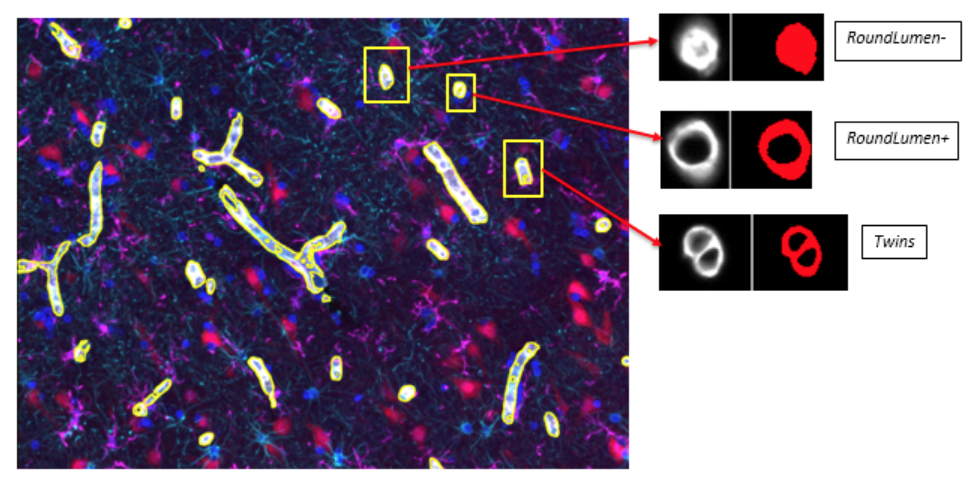
\includegraphics[width=1.0\textwidth]{img/morphologies}
\caption{Depiction of the different morphologies in the natural data with respect to a multichannel image, overlaid with different protein markers. The three types of morphologies analyzed in this study is represented on the right.}
\label{fig:morphologies}
\end{figure}

The number of instances of the three different types of morphologies are depicted in Table \ref{table:classes}.
\begin{table}[ht!]
\caption{Distribution of vascular morphologies}
\centering
\begin{tabular}{ | c | c |} 
\hline
\textit{RoundLumen-} & 689 \\ 
\hline
\textit{Roundlumen+} & 3427 \\ 
\hline
\textit{Twins} & 266 \\ 
\hline
Total & 4382 \\ 
\hline
\end{tabular}
\label{table:classes}
\end{table}

\subsection{Virtual data}
The construction of the artificial model starts with defining a set of control points in three dimensional Cartesian coordinates. The control points reflect the basic structure that the blood vessel is supposed to represent. This is followed by interpolating between the points using a 3D cubic spline interpolator. This forms the skeleton or the center line that represents the center or the lumen of the blood vessel and is shown in Fig. 2(a). The 3D volume of the blood vessel is constructed after this step. We first define a number of parameters; the inner radius of the blood vessel (r); the outer radius (R). The number of sampling points along the spline (N); the number of sampling points in the radial direction (Nr). At each sampling point; we define a circular disk along the z-axis; by randomly perturbing the values of r and R. We also define an intensity model for the blood vessels depicted in Eq. \ref{eq:1}. From the natural images, it seems that the intensity is high in the periphery of the blood vessel and decays towards the lumen and as we move away from the periphery. We model this using an exponential decay in the following form:

\begin{equation}
I(d) = I_{max} \exp(- \alpha |r\prime - d|)
\label{eq:1}
\end{equation}


where, $I_{max}$  is the maximum intensity, is the calibration coefficient (in mm-1 units), $r\prime=(R+r)/2.$ $d$ is the distance from the center of the lumen. At each point on the disc, we define the voxel density as a normal distribution with mean $I(d)$ and standard deviation 0.01. This is followed by formulating the rotation matrix by calculating the angle between the tangent to the spline at that sampling point and the z-axis. The points corresponding to each point on the disc are therefore mapped or rotated along the curve by multiplying the coordinates with the rotation matrix. An example of this rotation is depicted in Fig. \ref{fig:3D_model}(b). We then discretize the coordinates such that we obtain an actual 3D image in the form of an array. This is depicted in Fig. \ref{fig:3D_model}(c). The intensity values are normalized and assigned to the corresponding discretized points in the 3-dimensional array. The volume rendered version of the 3D image is depicted in Fig. \ref{fig:3D_model}(d). Therefore, by changing the parameters of the model we can build several different 3D images and slice it at various angles to mimic the natural tissue cross sections at various depths and angles. Some examples the various models are depicted in Fig. \ref{fig:slicer}.

\begin{figure}[ht!]
\centering
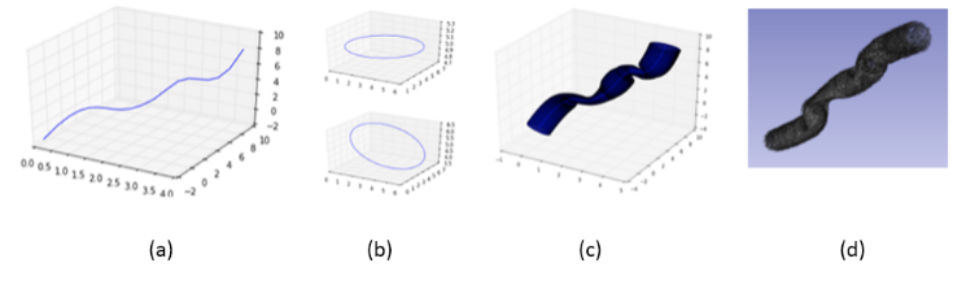
\includegraphics[width=1.0\textwidth]{img/3D_model}
\caption{Development of the 3D virtual model}
\label{fig:3D_model}
\end{figure}

\begin{figure}[ht!]
\centering
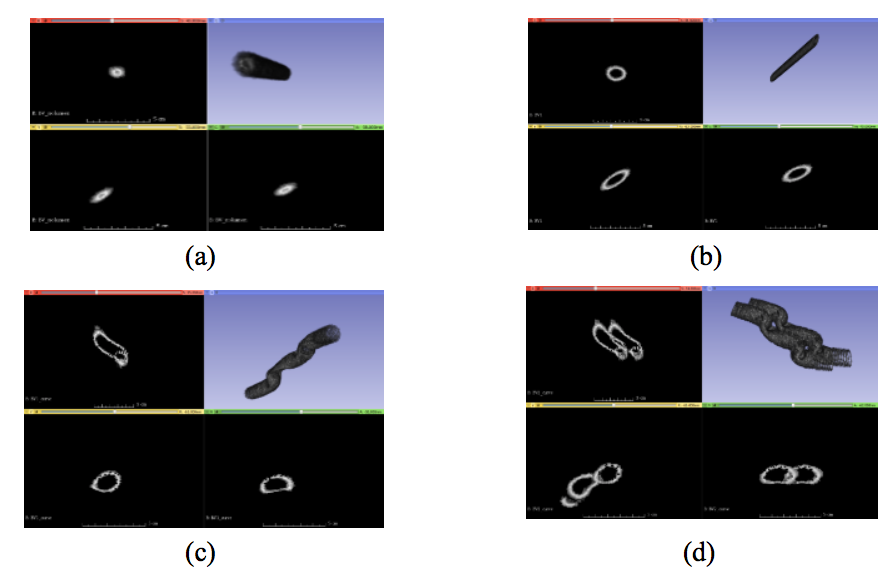
\includegraphics[width=1.0\textwidth]{img/slicer}
\caption{3D virtual models and their corresponding projections along different planes of view (a) Linear model of \textit{RoundLumen-} (b) Linear model of \textit{RoundLumen+} (c) Non-linear model of \textit{RoundLumen+} (d) Non-linear model of \textit{Twins}}
\label{fig:slicer}
\end{figure}

The process of construction of the different types of morphologies in blood vessels is the same as that explained above. Fig.  \ref{fig:slicer}(a) is a blood vessel with a no lumen (\textit{RoundLumen-}) and a linear skeleton. The control points are chosen such that they lie on the major diagonal of the unit cube; i.e. on the line x=y=z in Cartesian coordinates.  Figures  \ref{fig:slicer}(b) and  \ref{fig:slicer}(c) are blood vessel with a single lumen having linear and non-linear structures respectively. Fig.  \ref{fig:slicer}(d) is a model of a \textit{Twin}. As we can see from the cross-sectional views, we obtain different types of morphologies that are similar to actual morphologies in the natural images. A very simple way of creating these multi-vessel structures is by perturbing or shifting the sampling points of the skeleton along a random direction. For example; to come up with a model of \textit{RoundLumen-}, we simply set the inner radius r to 0. As shown in Fig. 3; the different morphologies that commonly occur naturally can be generated. As explained in the introduction; this serves as a viable alternative to using natural data for training convolutional networks.

\section{Methods}

A convolutional neural network is a type of artificial neural network in which are inspired by the organization of the 
animal visual cortex. CNNs consist of multiple neuron collections which process portions of the input image called receptive fields. The outputs are then tiled so that the input regions overlap and this in turn produces a better representation of the original image. This is what makes CNNs translation invariant. 
The CNN is made up of four types of layers: the input layer, the convolutional layer, the non-linear layer, the pooling layer; and the fully connected layer. The input layer is where the networks accept the images.  The images consist of raw pixel values depicted by width, height and the number of channels.  The convolutional layer will compute the output of the neurons that are connected to local regions in the input, each computing a dot product between their weights and a receptive field. The non-linear layer is the activation function responsible for introducing the non-linearity in the model. The various types of non-linear functions include the sigmoid, the tanh, and the rectified linear unit. The pooling layer performs a down sampling operation. The high-level reasoning in the neural network is done by fully connected layers.  Their activations can be performed by simple matrix multiplication.
In this work, we use the pre-trained convolutional neural networks as a feature extractor. This network consists of weights trained on the ImageNet dataset. We extract the 6th layer in the network which is a 4096-dimensional vector as a representation of the image. This may be considered as a transfer learning model because we transfer the weights learnt from another domain to blood vessel recognition. We use a pre-trained neural network called AlexNet \cite{krizhevsky2012imagenet} to extract features from the data. 

We perform an experiment to show that pre-trained CNNs are efficient in representing the vascular morphology. The experiment is performed on the natural data where 33 \% of the data is held out as test data and the rest is used for training. Two models are developed. One of them uses the visual bag of words (VBW) \cite{yang2007evaluating} feature extraction method to extract the features; the other uses the AlexNet architecture to extract the features. A three-class classification (one vs rest) is performed using the logistic regression classifier. The accuracy, f1-score, precision and recall calculated on the same test data are reported for comparison.

\begin{table}[ht!]
\centering
\caption{Comparison of feature extraction methodologies}
\begin{tabular}{ | c | c | c | c | c |} 
\hline
Feature extractor  & Accuracy	& f1-score	 & Precision & Recall \\ 
\hline
\textit{AlexNet} & 91.92 & 91.93 & 91.98 & 91.92 \\ 
\hline
\textit{VBW} & 78.38	& 77.38 & 	76.71 & 78.38 \\
\hline
\end{tabular}
\label{table:FE}
\end{table}

The results in Table \ref{table:FE} show that pre-trained convolutional neural networks are a good choice for representation of vascular morphology.

\section{Experiments and results}
Features are extracted using the AlexNet architecture which is trained on the ImageNet \cite{deng2009imagenet} database. The weight parameters are used to extract the features in a feedforward manner. This is called transfer learning. 33 \% of the natural data is held out as test data. All the experiments are performed on this dataset for maintaining consistency in the results. 
A filtering technique is introduced to appropriately extract slices from the 3D volumes. This is done by obtaining the probabilities of the artificial data using a model trained on the natural training data. The probabilities of the corresponding images are then sorted and the images with the highest probabilities are selected. This is a way to boost the artificial model.  The filtered virtual data is then used to retrain the classifier. Examples of both the natural and artificial data are represented in the Fig. \ref{fig:slices}.

\begin{figure}[ht!]
\centering
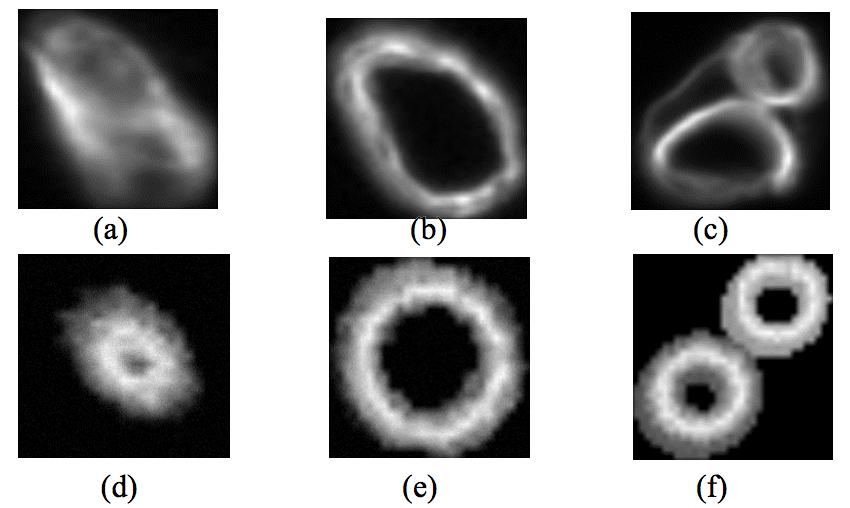
\includegraphics[width=1.0\textwidth]{img/slices}
\caption{ Examples of vessel classes \textit{RoundLumen-} (a/d), \textit{RoundLumen+} (b/e) and \textit{Twins} (c/f) for natural (a/b/c) and virtual data (d/e/f)}
\label{fig:slices}
\end{figure}

A hierarchical classification is performed to first classify the single blood vessels from blood vessels that bundled in pairs i.e \textit{RoundLumen} vs \textit{Twins}. The second classification task involves distinguishing between \textit{RoundLumen-} and \textit{RoundLumen+}. We perform three different types of training to demonstrate our proposed methods. The first type of training is done with only the naturally occurring data. The second type of training data consists only of the artificial data that has been filtered by the natural model as explained before. Finally, the third type consists of both the artificial and natural training samples. We refer to this as Mixed. All the results are reported on the held out 33 \% of the natural data. The accuracy, f1-score, precision, recall and receiver operating characteristic (ROC), and precision-recall (PR) curves are reported in the following tables and figures for each of the two classification tasks. 

\begin{table}[ht!]
\centering
\caption{Results of binary classification between \textit{RoundLumen} and \textit{Twin}}
\begin{tabular}{ | c | c | c | c | c |} 
\hline
Data & Accuracy & f1-score & Precision & Recall \\ 
\hline
\textit{Artificial} & 92.81& 59.36	& 45.24 & \textbf{86.36} \\ 
\hline
\textit{Natural} & 96.34& 71.03& 68.42& 73.86 \\
\hline
\textit{Mixed} & \textbf{97.71} & \textbf{81.76} & \textbf{79.57} & 84.01 \\
\hline
\end{tabular}
\label{table:results}
\end{table}


\begin{figure}[ht!]
    \centering
    \begin{subfigure}[t]{0.5\textwidth}
     \centering
       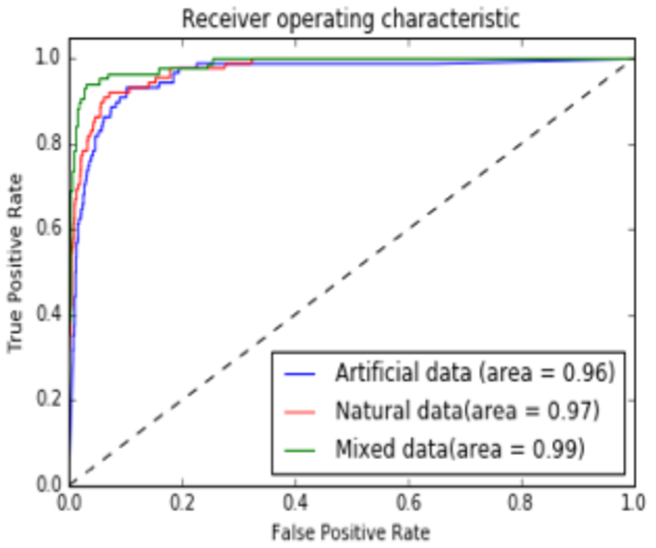
\includegraphics[width=1.0\linewidth]{img/single_twins_ROC.pdf}
  \caption{ROC curve}
        \label{fig:ROC1}   
    \end{subfigure}%
    \begin{subfigure}[t]{0.5\textwidth}
        \centering
          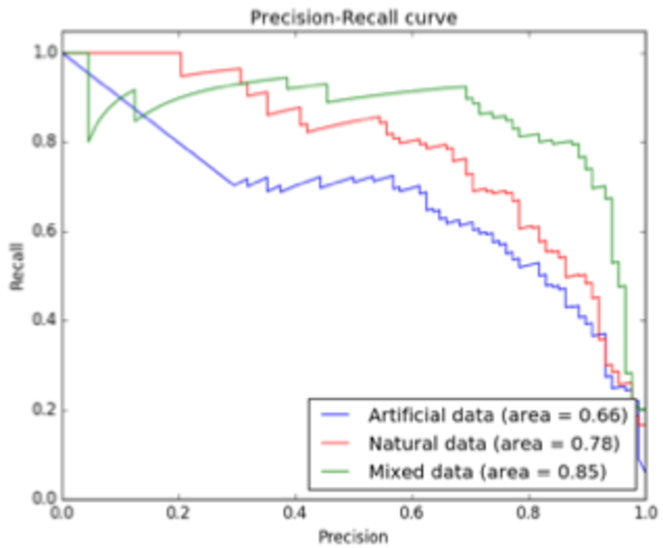
\includegraphics[width=1.0\linewidth]{img/single_twins_PRC.pdf}
  \caption{PR curve }
        \label{fig:PRC1}
    \end{subfigure}%
    \caption{Plots of the receiver operating characteristics (ROC) curve and the precision recall (PR) curve of the classification between \textit{RoundLumen} and \textit{Twins} along with the area under the curves (AUC) for the three experiments denoted as legends in the plots. From the nature of the curves, and the values of the AUC, we conclude that combining the using \textit{mixed} data performs better than using the \textit{Natural} data or the \textit{Artificial data} in isolation.}
    \label{fig:ROC_PRC1}
\end{figure}


\begin{table}[ht!]
\centering
\caption{Results of binary classification between \textit{RoundLumen-} and \textit{RoundLumen+}}
\begin{tabular}{ | c | c | c | c | c |} 
\hline
Data & Accuracy & f1-score & Precision & Recall \\ 
\hline
\textit{Artificial} & 98.38 & 99.02 & 99.38 & 98.67 \\ 
\hline
\textit{Natural} & 96.34& 71.03& 68.42& 73.86 \\
\hline
\textit{Mixed} & \textbf{98.60} &  \textbf{99.16} & \textbf{99.29} & \textbf{99.03} \\
\hline
\end{tabular}
\label{table:results1}
\end{table}


\begin{figure}[ht!]
    \centering
    \begin{subfigure}[t]{0.5\textwidth}
     \centering
       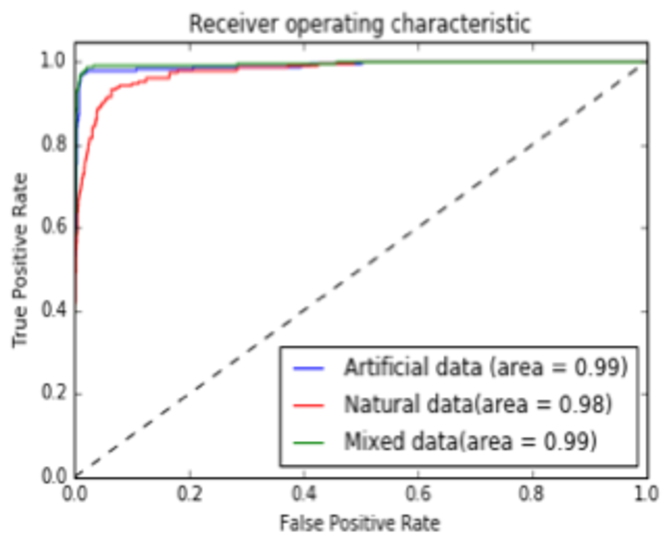
\includegraphics[width=1.0\linewidth]{img/roundlumens_ROC.pdf}
  \caption{ROC curve}
        \label{fig:ROC2}   
    \end{subfigure}%
    \begin{subfigure}[t]{0.5\textwidth}
       \centering
          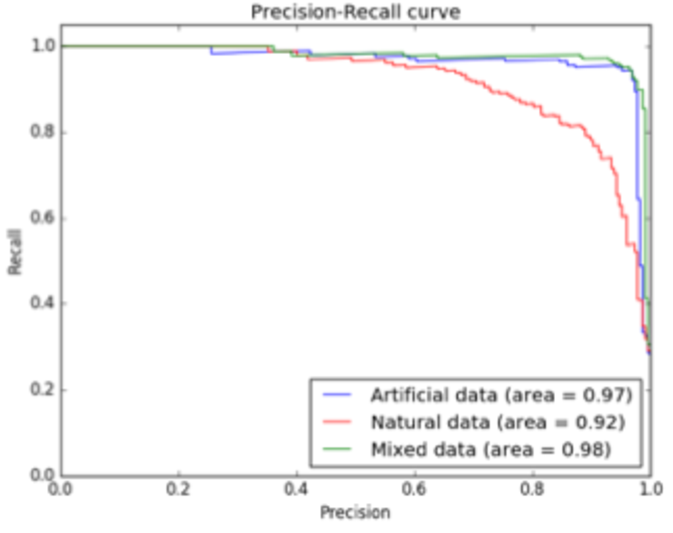
\includegraphics[width=1.0\linewidth]{img/roundlumens_PRC.pdf}
  \caption{PR curve }
        \label{fig:PRC2}
    \end{subfigure}%
    \caption{Plots of the receiver operating characteristics (ROC) curve and the precision recall (PR) curve of the classification between \textit{RoundLumen+} and \textit{RoundLumen-} along with the area under the curves (AUC) for the three experiments denoted as legends in the plots. From the nature of the curves, and the values of the AUC, we conclude that combining the using \textit{mixed} data performs better than using the \textit{Natural} data or the \textit{Artificial data} in isolation.}
    \label{fig:ROC_PRC2}
\end{figure}

The ROC and PR curves are calculated using the minority class in both the classification tasks, i.e. \textit{Twins} for the first classification task and \textit{RoundLumen-} for the second task.
From Table \ref{table:results}, we can see that the artificial data captures the differences between the two classes. It is also able to identify \textit{Twins}, which is the minority class in Task 1, from the high recall. Therefore, the results are boosted when we combine both the artificial and natural data. In addition, the ROC and PR curves in Figs. \ref{fig:ROC_PRC1} confirms our hypothesis that virtual data may be used for building the models. The naturally trained model performs better than the virtual trained model. However, as we can see from the ROC curves, the model built from the mixed data improves the performance. Table \ref{table:results1} and Fig.  \ref{fig:ROC_PRC2} presents the corresponding results for the second classification task. In this case, we see that the virtual data performs better than the natural data and boosts the performance when trained on its own or in union with the natural data.

\section{Conclusions}
We have shown that the use of deep learning algorithms  trained with a mixture of virtual and natural data  results in a more accurate prediction of vasculature morphologies than the use of standard feature extraction methods (such as visual bag of words). The methodology of complementing natural data with synthetic samples holds potential for becoming a standard approach in deep learning with unbalanced datasets. In neuroscience, it could be applied to help elucidate the underlying mechanisms of common neurological degenerative diseases.
\chapter{A MACHINE LEARNING APPROACH TO QUANTIFYING NOISE IN MEDICAL IMAGES}
\label{chap:automated}

\let\thefootnote\relax\footnotetext{
This chapter previously appeared as:
A. Chowdhury, K.~S. Aggour, S.~M. Gustafson, B. Yener,
``A Machine Learning Approach to Quantifying Noise in Medical Images.''
\emph{Medical Imaging 2016: Digital Pathology},
vol. 9791, pp. 979110U, 2016.}

%%% INTRODUCTION
\section{Introduction}

As advances in medical imaging technology are resulting in significant growth of biomedical image data, new techniques are needed to automate the process of identifying images of low quality. Automation is needed because it is very time consuming for a domain expert such as a medical practitioner or a biologist to manually separate good images from bad ones. While there are plenty of de-noising algorithms in the literature, their focus is on designing filters which are necessary but not sufficient for determining how useful an image is to a domain expert.
Thus a computational tool is needed to assign a score to each image based on its perceived quality. In this paper, we introduce a machine learning-based score and call it the Quality of Image (QoI) score. The QoI score is computed by combining the confidence values of two popular classification techniques support vector machines (SVMs) and Na�ve Bayes classifiers.
We test our technique on clinical image data obtained from cancerous tissue samples. We used 747 tissue samples that are stained by four different markers (abbreviated as CK15, pck26, E\_cad and Vimentin) leading to a total of 2,988 images. The results show that images can be classified as good (high QoI), bad (low QoI) or ugly (intermediate QoI) based on their QoI scores. Our automated labeling is in agreement with the domain experts with a bi-modal classification accuracy of 94 \%, on average. Furthermore, ugly images can be recovered and forwarded for further post-processing.

%%% Data
\section{Data}

The data we use is in the form of microscopic images. The colon cohort in this analysis was collected from the Clearview Cancer Institute of Huntsville Alabama from 1993 until 2002, with 747 patient tumor samples collected as formalin-fixed paraffin-embedded specimens. The median follow-up time of patients in this cohort is 4.1 years, with a maximum of over ten years. Stage 2 patients comprise 38 \% of this cohort, stage 1 and 2 combined are 65 \% of the total patients. We have stained and processed 747 CRC subjects described above on tissue microarrays for 63 target proteins of consequence to cancer biology and ancillary image processing and analysis. A full description of materials and methods was described recently in \cite{gerdes2013highly}.
The images are stained with four different markers. The markers are Ecadherin (E\_cad), pan-Keratin (pck26), Keratin15 (CK15) and Vimentin. The first three markers stain epithelial cells in the tissue, while Vimentin stains mesenchymal cells - a complementary set of cells in the image obtained from the same tissue sample, as shown in Fig. 1. The raw dataset consists of 747 tissue samples and each tissue sample has four images from each marker; resulting in a total of 2,988 images. Since images with the Vimentin marker provides complementary information to the other three markers; we do not use this marker for our analysis and prediction. We do, however, perform preliminary noise reduction on all four markers. The images marked with E\_cad have the least amount of noise associated with them. Images stained with pck26 and CK15 have more noise and undesirable artifacts in them.

\begin{figure}[H]
\centering
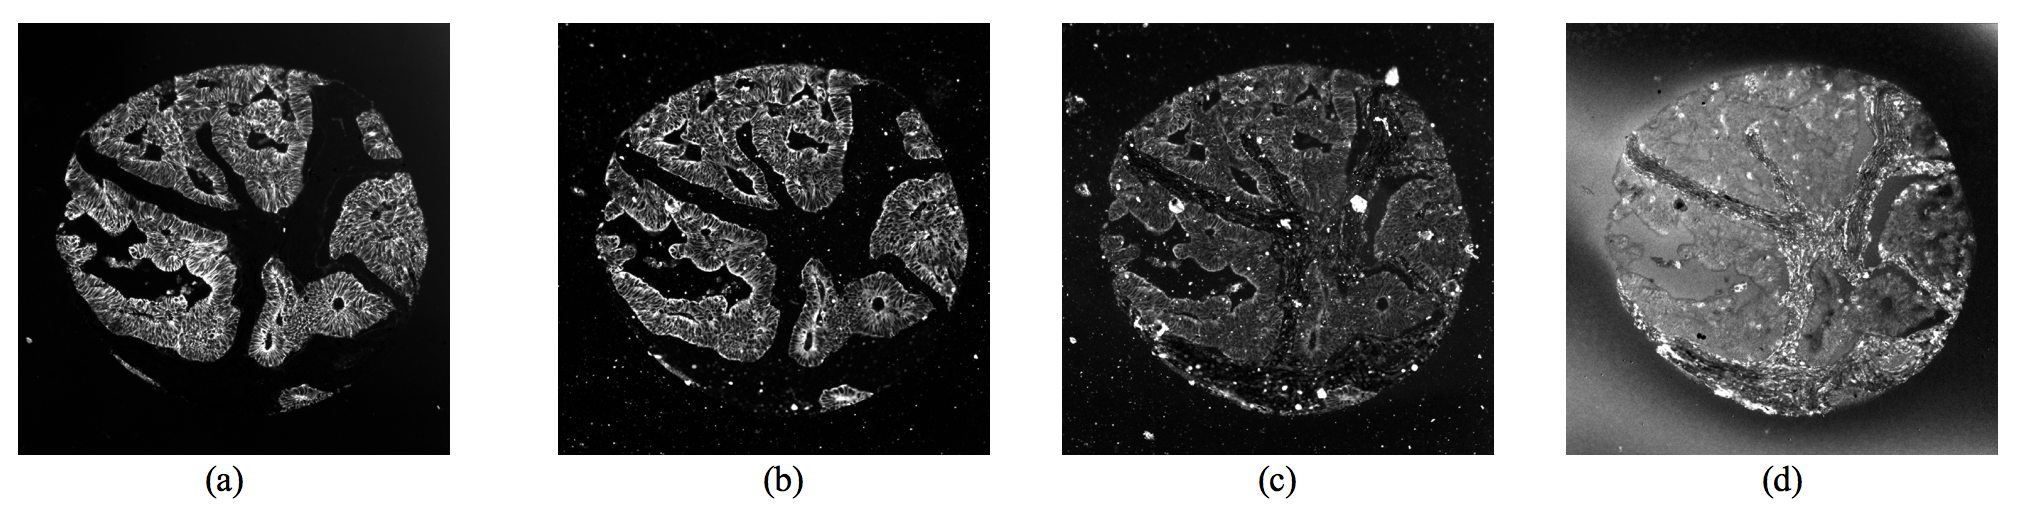
\includegraphics[width=1.0\textwidth]{img/SPIE_example_images}
\caption{Examples of a single colon tumor tissue sample stained with (a) E\_cad (b) pck26 (c) CK15 (d) Vimentin}
\label{fig:SPIE_example_images}
\end{figure}

\subsection{Preliminary noise reduction}
We perform preliminary noise reduction on all four types of images using two techniques. We remove salt and pepper noise using median filtering \cite{huang1979fast} followed by removal of white blob-shaped artifacts using intensity thresholding. Fig. \ref{fig:SPIE_noise_reduction} represents an example of the noise reduction on an image from CK15.  The QoI score (defined in the next section) increases by 67.85 \% on average after noise removal. This shows that the QoI score provides a more accurate estimate after noise removal has been performed. Hence, this step is essential in the process.

\begin{figure}[H]
\centering
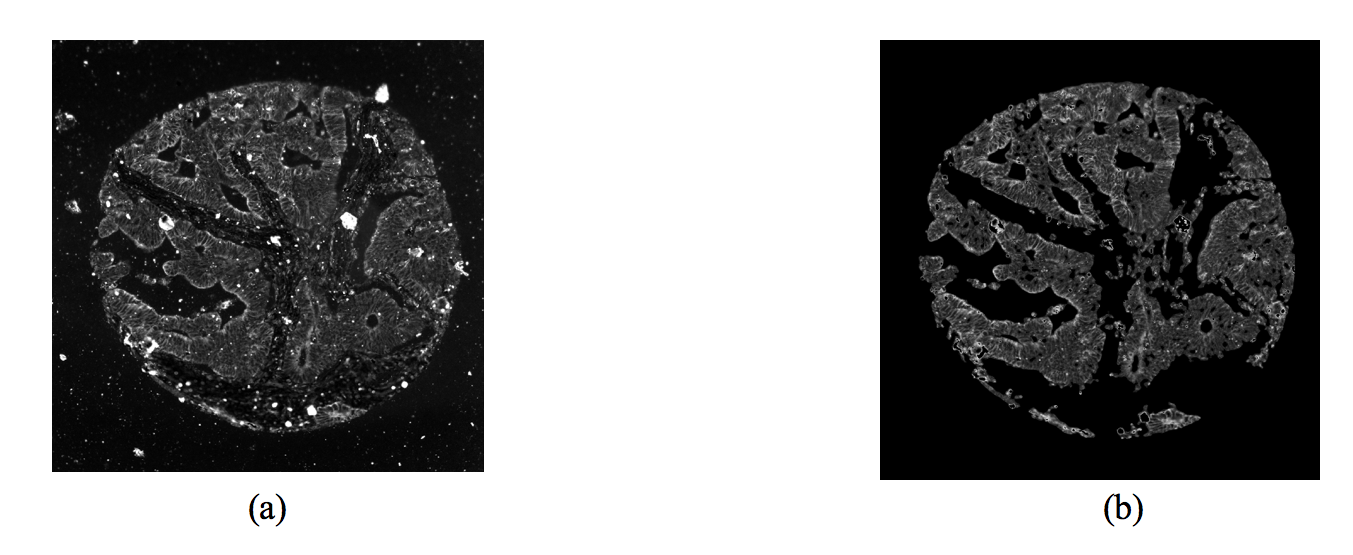
\includegraphics[width=0.9\textwidth]{img/SPIE_noise_reduction}
\caption{ Preliminary noise reduction on an image from CK15 (a) Original image (b) Noise-reduced image
}
\label{fig:SPIE_noise_reduction}
\end{figure}

\subsection{Combination of the three markers}
In addition to the three markers (CK15, pck26, and E\_cad) that we are working with; we use image analysis techniques to form a superimposition of the three markers in such a way that the different types of cells that the markers stain are all present in this one super image. We call this the combined marker. Diffusion like interference exists in the noisy images. The combined image is a way to reduce this kind of noise. The QoI score (defined in the next section) of the combined image is on an average higher (10.76 \%) than the QoI scores of images stained with the rest of the markers for a particular tissue sample. The superposition is performed after preliminary noise elimination. It is done by taking the minimum pixel intensity value among the three images in low intensity regions. We take the maximum intensity value in other regions. An example of this is shown in Fig. \ref{fig:SPIE_combination}. This combination increases the size of the data set; which is inherently imbalanced. It also aids in the recovery of images from the \textit{ugly} class based on the QoI results, as we shall see in the following section.

\begin{figure}[H]
\centering
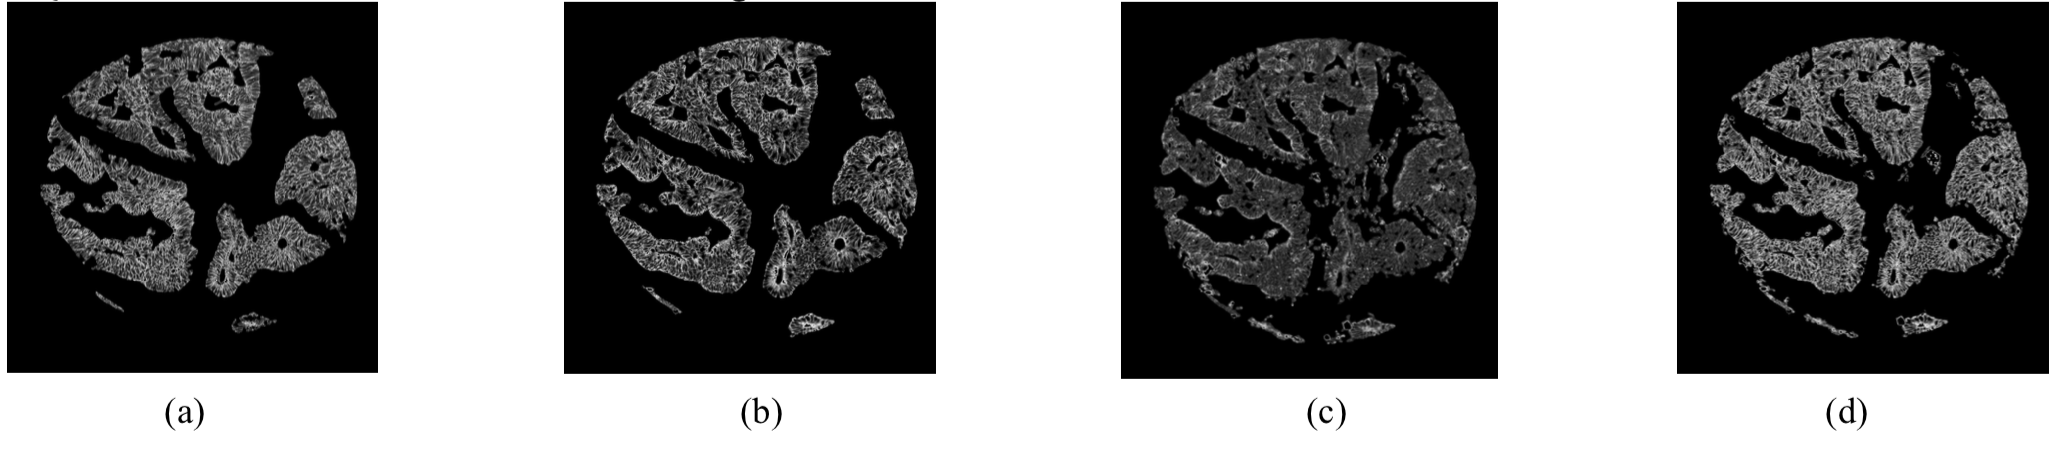
\includegraphics[width=1.0\textwidth]{img/SPIE_combined}
\caption{Images from (a) E\_cad, (b) pck26 and (c) CK15 are used to form the (d) Combined image}
\label{fig:SPIE_combination}
\end{figure}

\subsection{Feature extraction}

We quantify the information in the four markers (E\_cad, pck26, CK15 and Combined) by creating 24 domain-specific features. Features are based on gray-level intensity values, and texture information \cite{haralick1979statistical, haralick1973textural} in the images. 
%The features are shown in Table \ref{table:SPIE_features}.

%\begin{center}
%\begin{longtable}{ | m{6em} | m{10cm} |} 
%\caption{This table represents the various features extracted from the images. Features 9-23 are texture features based on the gray level co-occurence matrix of the image. The sum and difference features (features 14-20) are all measures of homogeneity and texture in the images. The information theoretic features are measures of correlation in the image. We embed a circular mask in the image to mimic the microscopic slide. This is what is meant as circle or circular mask whenever it is used in the formulation of a feature. More information about the features and their respective formulae can be found in \cite{haralick1979statistical, haralick1973textural}.}
% \hline
% Feature & Feature description \\ 
% \hline
% $1$ & Ratio of the size of the objects in the circle to area of the circle \\ 
% \hline
% $2$ & Ratio of the area of objects outside the circular mask to the area outside the circular mask \\  
% \hline
% $3$ & Mean of the gray level pixel values \\ 
% \hline
% $4$ & Second central moment (variance) of the gray level values in the image \\ 
% \hline
%$5$ & Third central moment (skewness) of the gray level values in the image \\ 
% \hline
%$6$ & Fourth central moment (kurtosis) of the gray level values in the image \\ 
% \hline
%$7$ & Energy of the image (quantifies the homogeneity in an image). \\ 
% \hline
%$8$ & Entropy of the image (measures the nonuniformity or complexity of the gray levels in the image) \\ 
% \hline
%$9$ & Texture entropy (measures the nonuniformity or complexity of the texture in the image) \\ 
% \hline
%$10$ & Angular second moment (a measure of homogeneity in the image) \\ 
% \hline
%$11$ & Inverse difference moment (a measure of local homogeneity in an image) \\ 
% \hline
%$12$ & Correlation (represents the linear dependencies of gray levels in the image) \\ 
% \hline
%$13$ & Contrast (a measure of how contrasting the gray level values are in the image) \\ 
% \hline
%$14$ & Sum of squares feature  \\ 
% \hline
%$15$ & Sum variance feature \\ 
% \hline
%$16$ & Sum entropy \\ 
% \hline
%$17$ & Difference average \\ 
% \hline
%$18$ & Difference variance \\ 
% \hline
%$19$ & Difference entropy \\ 
% \hline
%$20$ & Sum average \\ 
% \hline
%$21$ & Information theoretic feature  \\ 
% \hline
%$22$ & Information theoretic feature  \\ 
% \hline
%$23$ & Maximal correlation coefficient \\ 
% \hline
%$24$ & Average intensity of objects in the circle  \\ 
% \hline
% \endlastfoot
% \label{table:SPIE_features}
% \end{longtable}
%\end{center}
In addition to the features, labels are assigned to each image by domain experts based on the amount of noise in them. The label +1 is assigned if the image has some signal in it. This class is colloquially referred to as the \textit{good} class.  Images with a lot of noise in them where there is almost no signal are labelled as -1 or the \textit{bad} class.


\subsection{Data preprocessing}
We use 276x4 (1,104) images as the training set. The four markers (CK15, pck26, E\_cad, and combined) are used corresponding to each tissue sample. The rest of the images (1,884) are used for testing. The test and training sets were selected randomly, with 10-fold cross validation. The data is normalized such that the mean of every feature is 0 and standard deviation is 1.
Singular value decomposition (SVD) is performed to reduce the number of features from 24 such that it captures 95 \% of the information. This reduces the number of dimensions to 12.


\section{Methods and experiments}
In this section, we describe the methods that we used in our analysis of the images and also show the results that we achieved from the application of these methods on our data.

\subsection{Random undersampling}
The data in the two classes is imbalanced because the number of images in the \textit{good} class (images with high amount of signal) far outnumbers the number of instances in the \textit{bad} or noisy class. The ratio of imbalance is approximately 1:30. We perform random undersampling to redress the imbalance and ensure that the sizes of the two classes (good and bad) are the same.

\subsection{Classification and analysis}
We use two popular classification techniques - Support Vector Machines (SVM) and Na�ve Bayes classifiers. The accuracy of the Na�ve Bayes classifier for bi-modal classification on the test set is 96.38 \% and that of SVM is 91.27 \%.

\subsection{Quality of image score}
The models returned by the two classifiers are used to classify the test data as well as assign a score to each test image. The SVM classifier returns a margin value corresponding to each test point. This value is a representation of the distance of the instance from the classifier margin. The margin values are calibrated to fit a probability distribution using \cite{platt1999probabilistic}. The Na�ve Bayes classifier also returns a posterior probability that represents the membership of that point to that class. We combine these two values to form a score that is an indication of the quality of the image. We call this score the \textit{QoI score}. A high QoI score represents a high value of the signal and a small score value indicates that noise predominates the image. 
For image $i$, let $p_{i1}$and $p_{i2}$ be the probabilities returned by SVM and Na�ve Bayes classifiers respectively. Let $l_{i1}$ and $l_{i2}$ be corresponding labels returned the classifier models. The QoI score S is calculated as;

\begin{equation}
\begin{gathered} 
S \ =  \ \sqrt{p_{i1}p_{i2}} \ if \  l_{i1} = l_{i2}\\ 
     = \ 0.5 \ if \  l_{i1}  \neq l_{i2}\\ 
\end{gathered}
\label{eq:1}
\end{equation}

We take the geometric mean of the two scores that we get from each of the two classifiers, if the labelings are in agreement. A score of 0.5 is assigned if they are not. We tested other linear and non-linear functions as well. However, results were mostly invariant for these functions and we observed that the geometric mean was a better representation of the image quality. It is also intuitive that an image should be given the score 0.5 if the two classifiers do not predict the same thing. 
The scores of the test images are normalized such that they vary from 0 to 1; and they form a discrete distribution. The three sample images in Fig.5, (a), (b) and (c) received QoI scores of 0.9995, 0.5001, and 1.7595e-11 respectively using Eq. \ref{eq:1}.


\subsection{Defining the \textit{ugly} class}
In addition to the good and bad class, we observe that there exist some images, which have both quantities of signal and noise in relatively equal proportion. Classifying this kind of image as good or bad becomes very subjective. Therefore, it seems intuitive to define a third class, referred to as the ugly class. We define and extract this class based on the QoI scores in the following manner.
We plot histograms of these discrete distributions as shown in Fig. \ref{fig:ugly_distributions}. We can clearly see from the distributions that the scores form three distinct clusters. Therefore, we performed K-means clustering on the normalized score values with K=3. The cluster of images corresponding to the scores in the middle range is termed the ugly class. Images in the ugly class require further (possibly manual) processing. Thus, we are most interested in the images that are near the middle range, the images that we can recover. 
We threshold out the ugly images with the help of the middle cluster in K-means and using a threshold for scores. The thresholds are taken to be between 0.3 to 0.6. We have found that 7.22 \%, 9.77 \% and 29.30 \% of images in E\_cad, pck26 and CK15 respectively, lie in this middle cluster. The results are intuitive because the amount of noise increases progressively from E\_cad to CK15 to pck26. A number of things may be done with the images that belong to the ugly class. They may be forwarded to medical practitioners for inspection. Further noise elimination may also be performed, or as we have done, the ?combined? image could be used as a proxy for the images belonging to this ugly class. This is because the ?combined? image best captures the important information in the images stained with the three different markers.

 \begin{figure}[H]
\centering
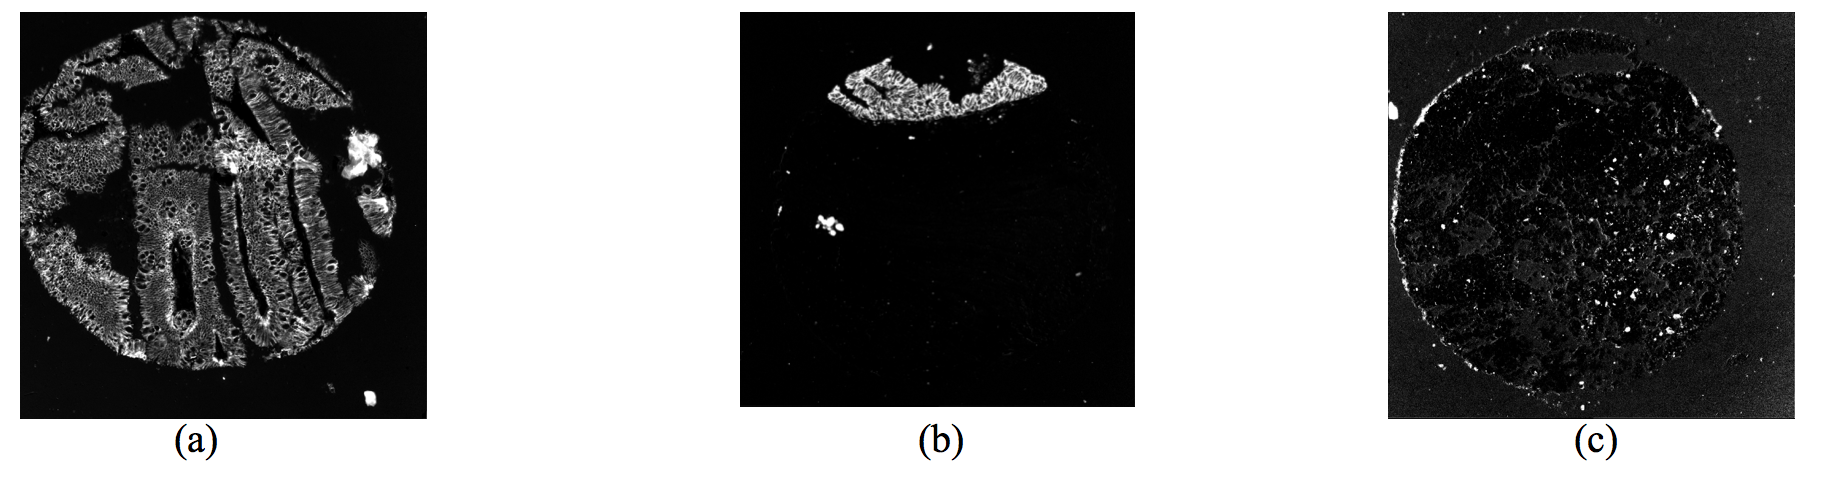
\includegraphics[width=1.0\textwidth]{img/ugly_samples}
\caption{Three sample images from E\_cad stained tissues}
\label{fig:ugly_samples}
\end{figure}

 \begin{figure}[H]
\centering
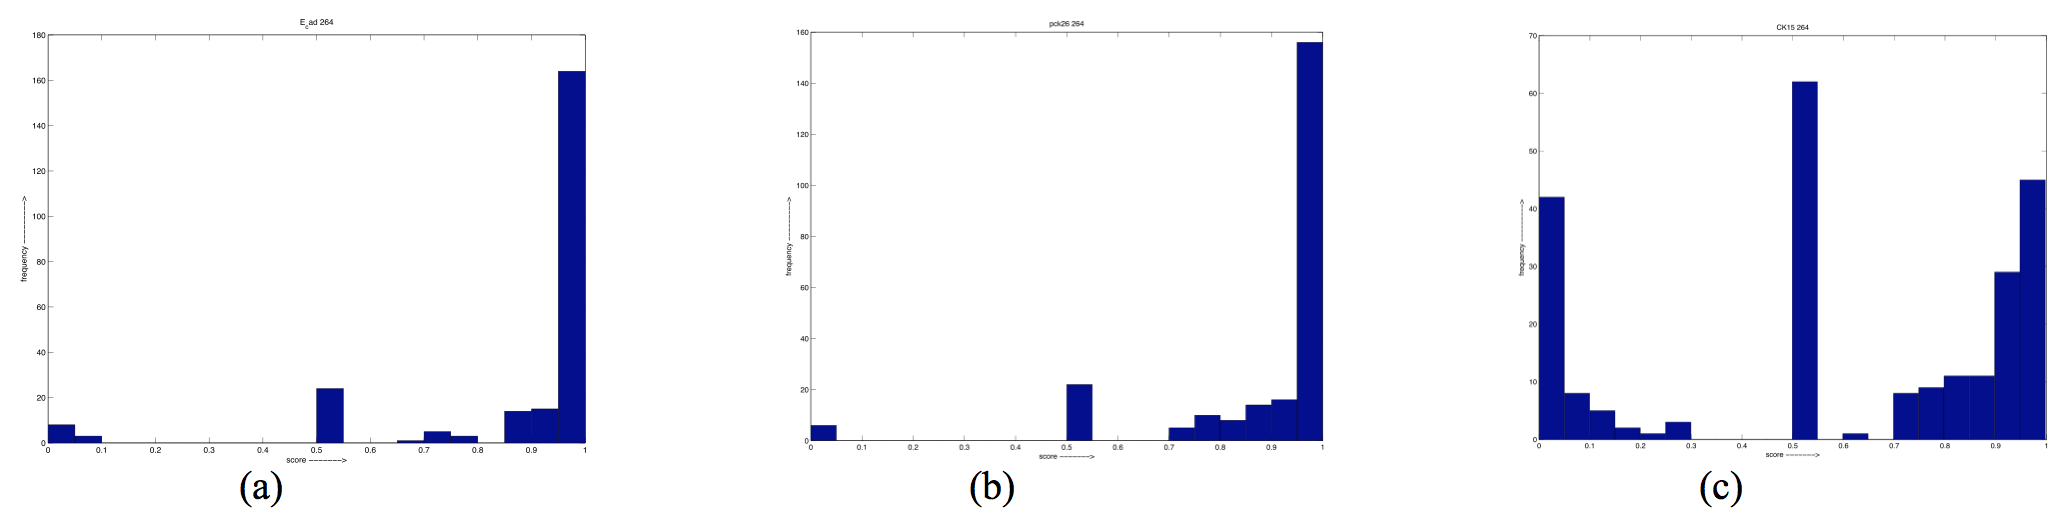
\includegraphics[width=1.0\textwidth]{img/ugly_distributions}
\caption{Discrete distributions of QoI scores for (a) E\_cad (b) pck26 (c) CK15}
\label{fig:ugly_distributions}
\end{figure}

\section{Conclusions}
We introduce in this paper a novel way to combine SVM and Na�ve Bayes classifiers to form an image quality score.  The score is based on the confidence of a data point with respect to the classifier margin; and the distribution of the data captured by the Na�ve Bayes classifier. Images that have high or low information content are easy to label as good or bad respectively. A labeling of the ugly class becomes dependent on the observer. Therefore computing a score is a more natural way of extracting this third class of images. The score helps us retrieve images that may have been discarded by a simple binary classification; or may have gone unnoticed by a human eye. Also, we use image analysis techniques to form a combined image that tries to capture the signal from all three markers.


%\chapter{A NON-UNIFORM REFINEMENT APPROACH
FOR SOLVING ADJOINT PROBLEMS IN FUNCTIONAL
ERROR ESTIMATION AND MESH ADAPTATION}
\label{chap:refine}

%%% INTRODUCTION
\section{Introduction}

Adjoint-based error estimation
\cite{becker2001optimal, giles2003adjoint,
pierce2004adjoint, venditti2000adjoint,
venditti2002adjoint,
venditti2003adjoint,
prudhomme1999goal,
prudhomme2003practical,
fidkowski2011review,
connors2013method}
is a tool used in numerical simulation
to estimate the discretization error
in physically meaningful output quantities.
Combined with mesh adaptation, adjoint-based error
estimation also provides the ability to control the discretization
error. The process of adjoint-based error estimation
relies on the introduction of an auxiliary
\emph{adjoint problem}, which is constructed using
the solution to the original or \emph{primal problem}
of interest.

To obtain meaningful error estimates,
the solution to the adjoint problem must be
enriched in some manner. That is, it is
necessary to obtain a representation of the
adjoint solution in a richer space compared
to the space used for the primal problem.
Several strategies are commonly
to obtain an enriched adjoint representation.
These approaches include
solving the adjoint problem in a globally higher
order polynomial space
\cite{fidkowski2011output},
solving the adjoint problem on a uniformly
refined mesh \cite{burstedde2009parallel},
solving the adjoint problem in the same space
as used for the primal problem
and solving local patch-wise problems least
squares problems \cite{nemec2007adjoint} or
by performing patch-wise higher-order interpolation
\cite{becker2001optimal},
and enriching the adjoint solution via
variational multiscale methods
\cite{granzow2017output}.

Solving the adjoint problem in a globally higher
order polynomial or on a uniformly refined mesh
is a computationally expensive proposition. On the
other hand, solving the adjoint problem in the same
space as used for the primal problem and enriching
it via local patch-wise problems may not be guaranteed
to yield a more accurate adjoint solution. In this
chapter, we propose a simple compromise and solve the
adjoint problem on meshes obtained via non-uniform
refinement.

The remainder of this chapter is structured as follows.
First, we review adjoint-based error estimation for
functional quantities using two discretization levels,
a \emph{coarse} space and a \emph{fine} space. We then
review three choices for the fine space, obtained
by refinement of the mesh used for the coarse space.
The first choice is the standard uniform refinement
method, while the other two approaches form the fine
space via non-uniform refinement. In each of these
sections, we discuss the algorithm utilized to generate
the fine space. We then investigate the these three
approaches for adjoint enrichment for Poisson's equation
and conclude with a summary of the results.

%%% OUTPUT ERROR ESTIMATION WITH TWO DISCRETIZATION LEVELS
\section{Error Estimation with Two Levels}

\subsection{Error Estimates}

Let $\V^h$ and $\V^H$ denote finite dimensional spaces
such that $\V^H \subset \V^h$. We refer to $\V^h$
and $V^H$ as the \emph{fine} space and the \emph{coarse}
space, respectively. Let $\bs{R}^H : \mathbb{R}^N \to \mathbb{R}^N$
denote the system of (potentially nonlinear) algebraic equations
arising from a finite element discretization of a PDE on the
coarse space $\V^H$, such that the solution vector
$\bs{u}^H \in \mathbb{R}^N$ satisfies
%
\begin{gather}
\bs{R}^H(\bs{u}^H) = 0.
\label{eq:refine_residual_coarse}
\end{gather}
%
Similarly, let $\bs{R}^h : \mathbb{R}^n \to \mathbb{R}^n$
denote the system of algebraic equations arising from a finite
element discretization of the same PDE on the fine space
$\V^h$, such that
%
\begin{gather}
\bs{R}^h(\bs{u}^h) = 0,
\label{eq:refine_residual_fine}
\end{gather}
%
where $\bs{u}^h \in \mathbb{R}^n$ is the solution vector on
the fine space and $n > N$.

Let $J^H : \mathbb{R}^N \to \mathbb{R}$ denote a discrete
representation of a physically meaningful functional quantity
on the coarse space $\V^H$, and similarly let
$J^h : \mathbb{R}^n \to \mathbb{R}$ denote the functional
approximated on the fine space $\V^h$. Let
$\bs{u}^h_H := \bs{I}^h_H \bs{u}^H$ denote the prolongation of
the coarse space solution $\bs{u}^H$ onto the fine space
$\V^h$ via interpolation, where
$\bs{I}^h_H : \V^H \to \V^h$.

The functional evaluated on the fine space $J(\bs{u}^h)$
can be expanded in a Taylor series approximation about the
prolonged coarse space solution $\bs{u}^h_H$ as
%
\begin{gather}
J^h(\bs{u}^h) = J^h(\bs{u}^h_H) +
\left[ \frac{\partial J^h}{\partial \bs{u}^h}
\biggr|_{\bs{u}^h_H} \right]
(\bs{u}^h - \bs{u}^h_H) + \dots
\label{eq:refine_functional_taylor}
\end{gather}
%
Similarly, the residual system of equations evaluated
on the fine space $\bs{R}^h(\bs{u}^h)$ can be expanded
about the prolonged coarse space solution $\bs{u}^h_H$ as
%
\begin{gather}
\bs{R}^h(\bs{u}^h) = \bs{R}^h(\bs{u}^h_H) +
\left[ \frac{\partial \bs{R}^h}{\partial \bs{u}^h}
\biggr|_{\bs{u}^h_H} \right]
(\bs{u}^h - \bs{u}^h_H) + \dots
\label{eq:refine_residual_taylor}
\end{gather}
%
Using the governing relation \eqref{eq:refine_residual_fine} in the
residual Taylor expansion \eqref{eq:refine_residual_taylor} suggests
a first order approximation for the discretization error between the
spaces:
%
\begin{gather}
(\bs{u}^h - \bs{u}^h_H) \approx
- \left[ \frac{\partial \bs{R}^h}{\partial \bs{u}^h}
\biggr|_{\bs{u}^h_H} \right]^{-1}
\bs{R}^h(\bs{u}^h_H).
\label{eq:refine_disc_error_approx}
\end{gather}
%
Inserting the error approximation \eqref{eq:refine_disc_error_approx}
into the functional Taylor expansion \eqref{eq:refine_functional_taylor}
suggests the error estimate:
%
\begin{gather}
J^h(\bs{u}^h) - J^h(\bs{u}^h_H) \approx
- \left[ \frac{\partial J^h}{\partial \bs{u}^h}
\biggr|_{\bs{u}^h_H} \right]
\left[ \frac{\partial \bs{R}^h}{\partial \bs{u}^h}
\biggr|_{\bs{u}^h_H} \right]^{-1}
\bs{R}^h(\bs{u}^h_H),
\end{gather}
%
which can be re-written in terms of an \emph{adjoint} variable
$\bs{z}^h$ as
%
\begin{gather}
J^h(\bs{u}^h) - J^h(\bs{u}^h_H) \approx
- \bs{z}^h \cdot \bs{R}^h (\bs{u}^h_H),
\label{eq:refine_adjoint_error}
\end{gather}
%
where $\bs{z}^h \in \mathbb{R}^n$ is the solution to the
so-called \emph{adjoint problem} given by
%
\begin{gather}
\left[ \frac{\partial \bs{R}^h}{\partial \bs{u}^h}
\biggr|_{\bs{u}^h_H} \right]^T
\bs{z}^h
=
- \left[ \frac{\partial J^h}{\partial \bs{u}^h}
\biggr|_{\bs{u}^h_H} \right]^T.
\label{eq:refine_adjoint_problem}
\end{gather}

\subsection{A Simple a-priori Analysis}

Consider that the functional of interest
converges at the rate $k$, such that
$J - J^h(\bs{u}^h_H) = c H^k$ and
$J - J^h(\bs{u}^h) = c h^k$,
where $J$ is the exact value of the functional
quantity of interest. Assume that the fine space
is obtained via refinement of the coarse space.
Consider the ratio
%
\begin{gather}
\frac{J^h(\bs{u}^h) - J^h(\bs{u}^h_H)}
{J - J^h(\bs{u}^h_H)} \approx
\frac{ - \bs{z}^h \cdot \bs{R}^h(\bs{u}^h_H)}
{J - J^h(\bs{u}^h_H)}
\end{gather}
%
which, as $H \to 0$, will tend towards \cite{fidkowski2011review}
%
%% refine_alpha
\begin{gather}
\alpha := 1 - \left( \frac{h}{H} \right)^k.
\label{eq:refine_alpha}
\end{gather}
%

Let $\eta$ denote our approximation to the
functional error $J - J^h(\bs{u}^h_H)$.
Let $\I$ denote the effectivity index
given by
%
\begin{gather}
\I = \frac{\eta}{J - J^h(\bs{u}^h_H)}.
\label{eq:refine_effectivity}
\end{gather}
%
We would like error estimates
$\E$ that lead to effectivity indices of
$\I = 1$ as $H \to 0$. To achieve this, we scale
the two-level adjoint weighted residual estimate
\eqref{eq:refine_adjoint_error} by the inverse
of the factor $\alpha$, such that
%
\begin{gather}
\eta = - \frac{1}{\alpha}
\bs{z}^h \cdot \bs{R}^h(\bs{u^h_H})
\label{eq:refine_error_approx}
\end{gather}

%%% CHOICES FOR THE FINE SPACE
\section{Choices for the fine space}

%%% UNIFORM REFINEMENT
\subsection{Uniform Refinement}

\begin{figure}[ht!]
\centering
\begin{subfigure}{.5\textwidth}
\centering
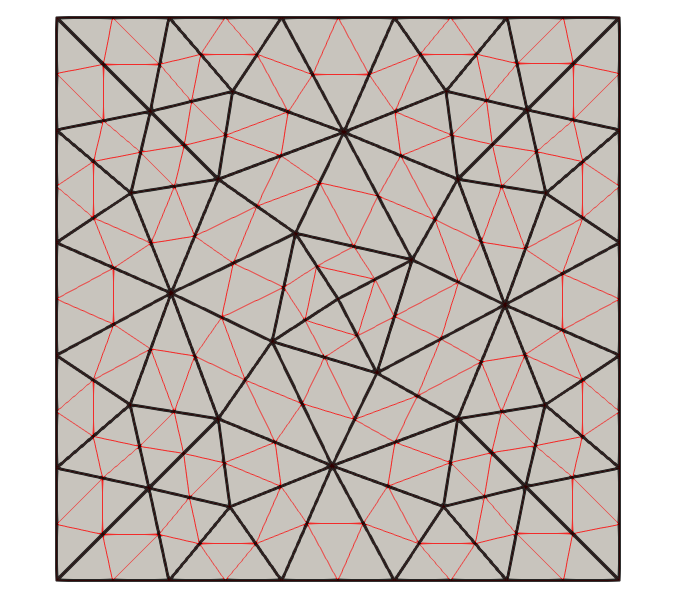
\includegraphics[width=.9\linewidth]{img/refine_unif_mesh.png}
\end{subfigure}%
\begin{subfigure}{.5\textwidth}
\centering
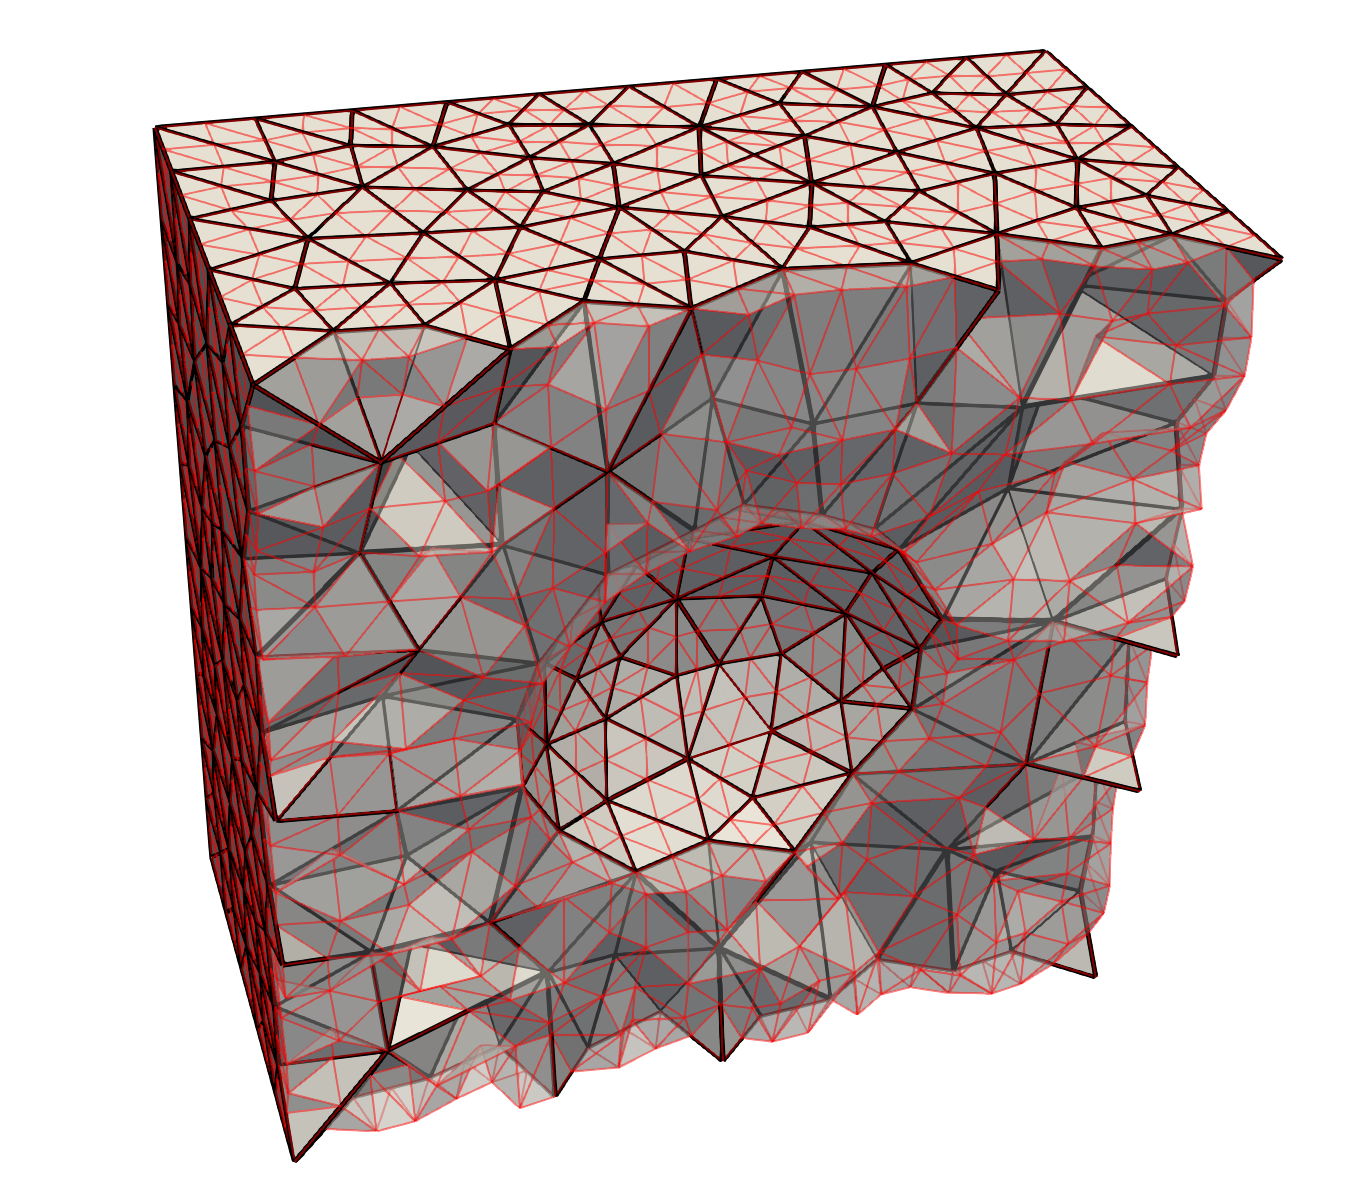
\includegraphics[width=.99\linewidth]{img/refine_unif_mesh_3D.png}
\end{subfigure}
\caption{Edges of a base mesh (black) and a nested mesh refined
with the Unif scheme (red) in two dimensions.}
\label{fig:unif_mesh}
\end{figure}

We first consider the traditional approach of using
a uniformly refined mesh to solve the adjoint problem.
We refer to this approach as the \textsc{Unif}
refinement approach.
To perform uniform refinement, every edge in the mesh
is marked for refinement. The algorithm for uniform
refinement is given in Algorithm \ref{alg:uniform_refine}.
Figure \ref{fig:unif_mesh} demonstrates an example of the
\textsc{Unif} refinement approach applied to a
base mesh. For the uniform refinement approach,
we naturally choose the ration $\frac{h}{H} = \frac12$,
leading to the scaling parameter
$\alpha = 1 - \left( \frac12 \right)^k.$

\begin{algorithm}
\caption{Uniform refinement algorithm}
\begin{algorithmic}
\For{ each edge $e$ in mesh $M$ }
\State mark edge $e$ for refinement.
\EndFor
\end{algorithmic}
\label{alg:uniform_refine}
\end{algorithm}

%%% LONG EDGE REFINEMENT
\subsection{Long Edge Refinement}

\begin{figure}[ht!]
\centering
\begin{subfigure}{.5\textwidth}
\centering
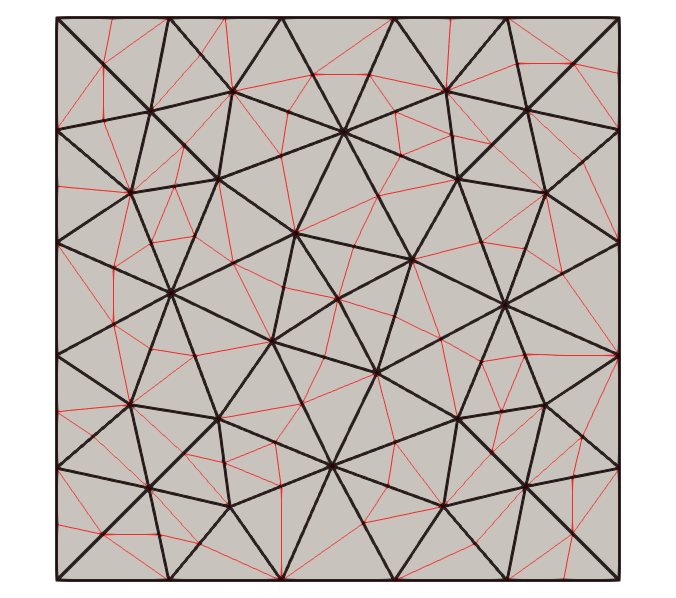
\includegraphics[width=.9\linewidth]{img/refine_long_mesh.png}
\end{subfigure}%
\begin{subfigure}{.5\textwidth}
\centering
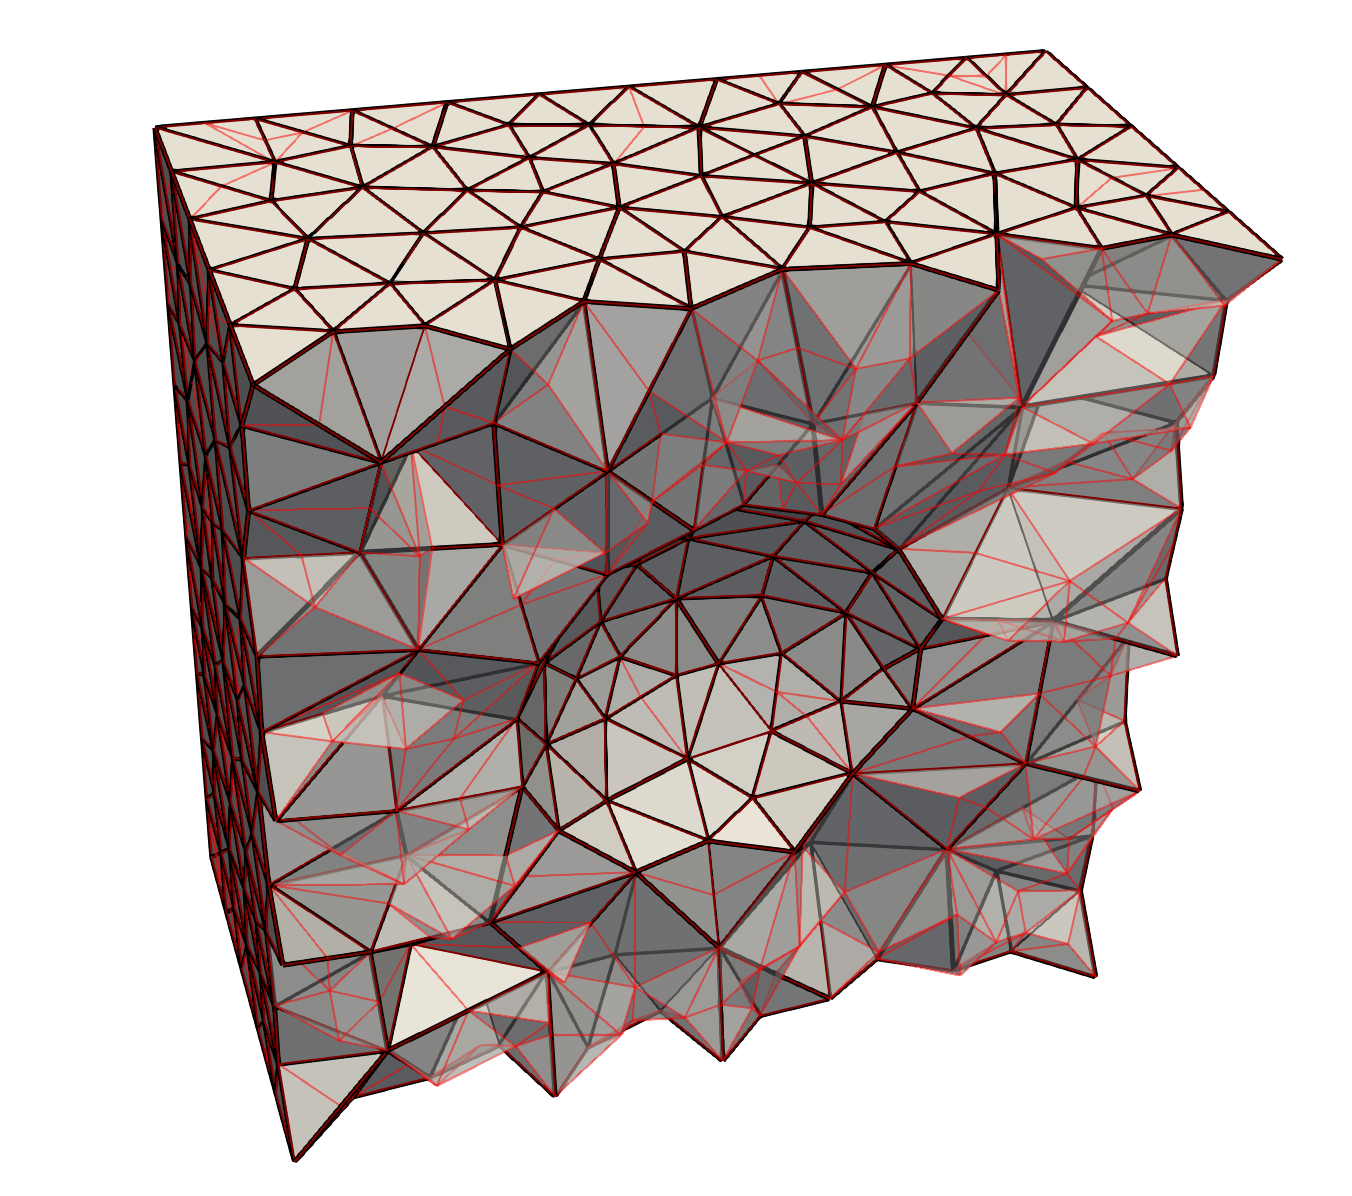
\includegraphics[width=.99\linewidth]{img/refine_long_mesh_3D.png}
\end{subfigure}
\caption{Edges of a base mesh (black) and a nested mesh refined
with the Long scheme (red) in two dimensions.}
\label{fig:long_mesh}
\end{figure}

Next, we consider an adaptive scheme that marks
the longest edge in each element for refinement.
We refer to this scheme as the Long edge
refinement scheme. The \textsc{Long} edge refinement
algorithm is outlined in Algorithm \ref{alg:long_refine}.
Figure \ref{fig:long_mesh} illustrates the
\textsc{Long} edge refinement algorithm applied to
a base mesh.

Not that, for the \textsc{Long} edge refinement
approach, some elements are split once, and others
are split multiple times. Thus, there is no global
single global ratio $\frac{h}{H}$. We approximate
this ratio by taking the average of all ratios
of nested element sizes to their parent element
size, given by
%
\begin{gather}
\frac{h}{H} \approx \frac{1}{n_{el}}
\sum_{e=1}^{n_{el}} \frac{h_e}{H_e},
\label{eq:refine_ratio}
\end{gather}
%
where $n_{el}$ is the total number of elements
in the nested mesh.

\begin{algorithm}
\caption{Long edge refinement algorithm}
\begin{algorithmic}
\For{ each element $el$ in mesh $M$ }
\For{ each edge $e$ in element $el$ }
\If { $e$ is longest edge in $el$ }
\State mark edge $e$ for refinement.
\EndIf
\EndFor
\EndFor
\end{algorithmic}
\label{alg:long_refine}
\end{algorithm}

%%% SINGLE EDGE REFINEMENT
\subsection{Single Edge Refinement}

\begin{figure}[ht!]
\centering
\begin{subfigure}{.5\textwidth}
\centering
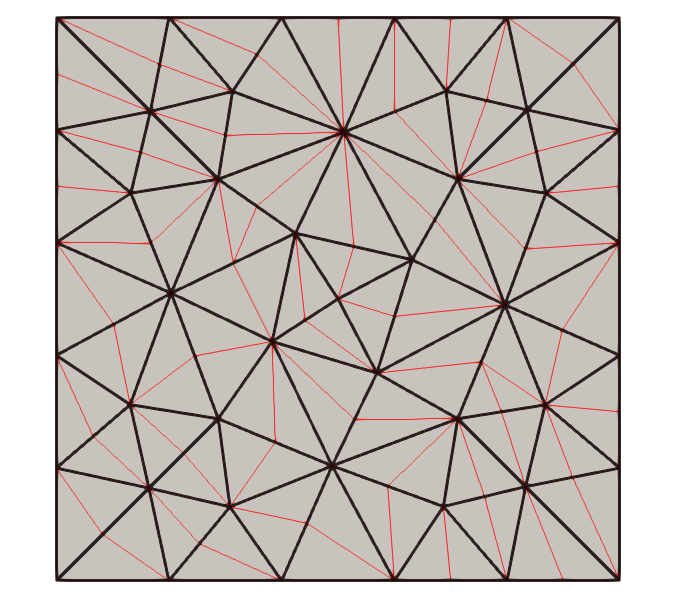
\includegraphics[width=.9\linewidth]{img/refine_single_mesh.png}
\end{subfigure}%
\begin{subfigure}{.5\textwidth}
\centering
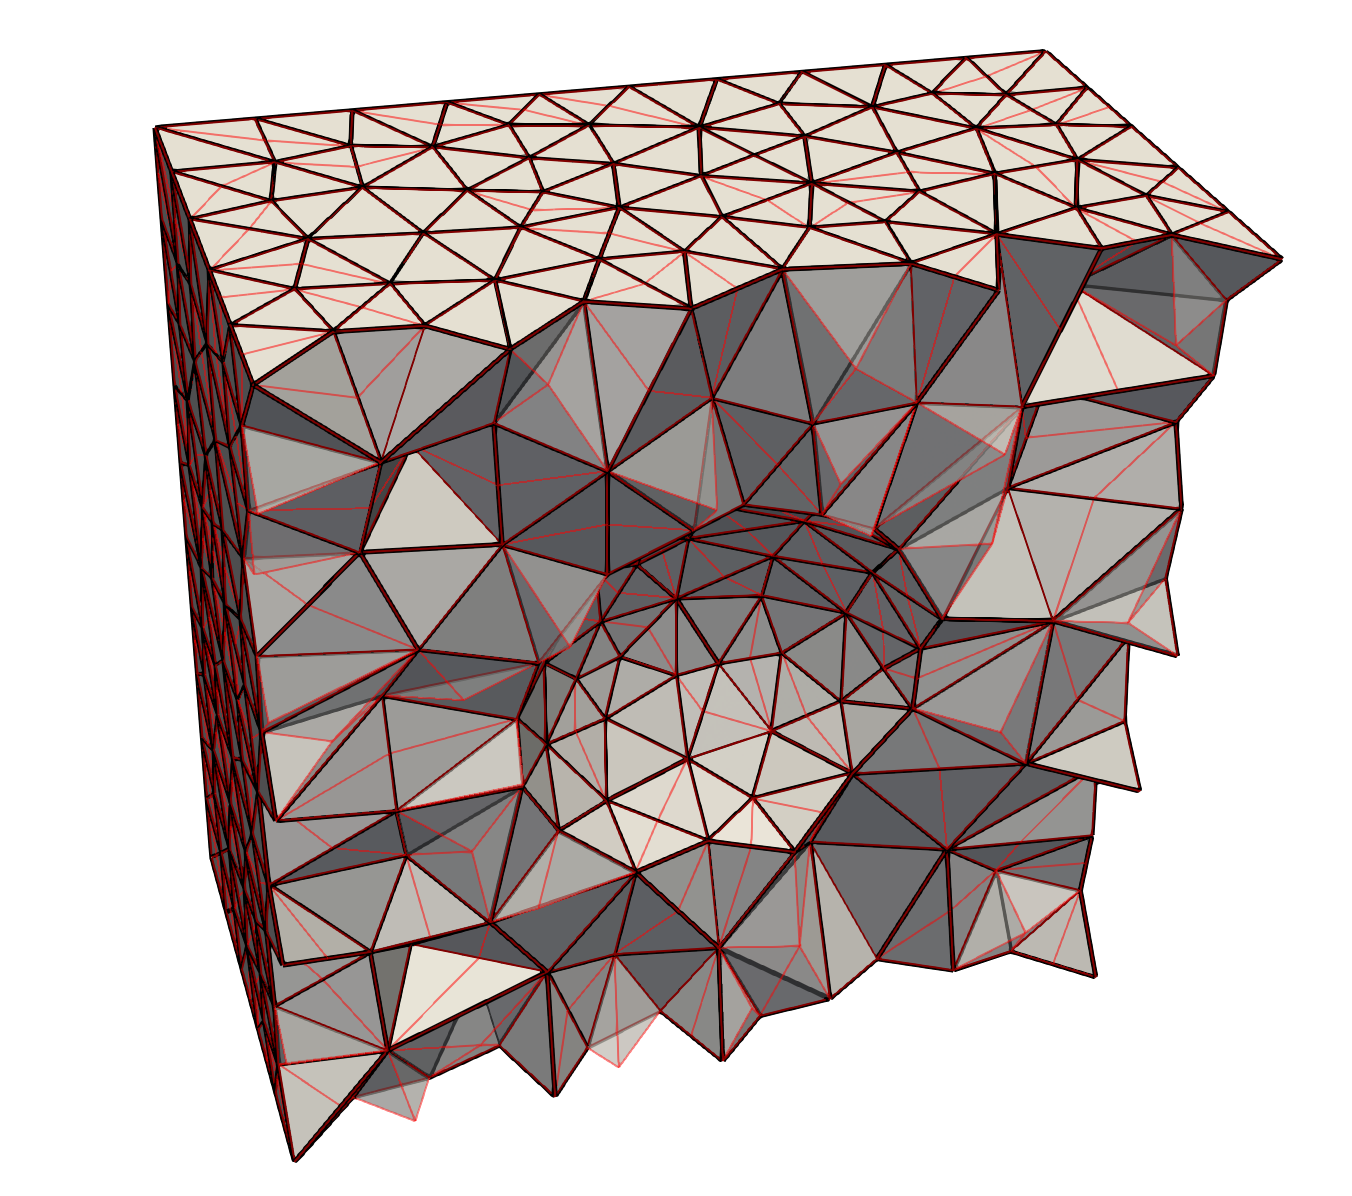
\includegraphics[width=.99\linewidth]{img/refine_single_mesh_3D.png}
\end{subfigure}
\caption{Edges of a base mesh (black) and a nested mesh refined
with the Single scheme (red) in two dimensions.}
\label{fig:single_mesh}
\end{figure}

Finally, we consider a cheap refinement alternative to
uniform refinement that attempts to only mark a single edge
in each element for refinement. We refer to this approach
as the \textsc{Single} edge refinement approach.
To perform single edge refinement, a traversal of all
edges in the mesh is performed. During this traversal,
the first edge encountered is marked for refinement
and the elements adjacent to that edge are tagged
as `visited'. As the edges in the mesh are traversed,
each element adjacent to the edge is checked to see
if it has already been encountered. If all adjacent
elements have not been encountered, then the edge
is marked for refinement.
After this process has completed, some elements may be
\emph{isolated}, in that they have still not been marked as `visited'.
Thus, for each element remaining that has not been marked as `visited',
we mark the first edge adjacent to the element for refinement.
The single edge refinement
algorithm is illustrated in \ref{alg:single_refine}.
Figure \ref{fig:single_mesh} demonstrates a mesh
resulting from the application of the single
edge refinement scheme. For the \textsc{Single}
scheme, we again approximate the ratio
$\frac{h}{H}$ with equation \eqref{eq:refine_ratio}.

\begin{algorithm}
\caption{Single edge refinement algorithm}
\begin{algorithmic}
\State initialize all elements to be `not visited'.
\For{ each edge $e$ in mesh $M$ }
\State let $S$ be the set elements adjacent to edge $e$.
\If{ each element in $S$ is `not visited' }
\State mark edge $e$ for refinement.
\For{ each element $el$ in $S$ }
\State mark element $el$ as `visited'.
\EndFor
\EndIf
\EndFor
\For{ each element $el$ in mesh $M$ }
\If{ $el$ is marked as `not visited' }
\State let $S$ be the edges adjacent to element $el$
\State mark the first edge $e$ in $S$ for refinement
\EndIf
\EndFor
\end{algorithmic}
\label{alg:single_refine}
\end{algorithm}

%%% MESH ADAPTATION
\section{Mesh Adaptation}

%%% ERROR LOCALIZATION
\subsection{Error Localization}

It is necessary to localize contributions to the 
total error $\eta$ to mesh entity level \emph{correction indicators}
to drive mesh adaptation. For finite volume and discontinuous
Galerkin finite element methods, it is common to consider the discrete
element-level adjoint weighted residuals of the form
$\bs{z}^h_e \cdot \bs{R}^h_e$, where the subscript $e$ denotes evaluations
over elements. However, for continuous finite elements, this approach
does not account for systematic inter-element cancellation
\cite{fidkowski2011review}, which could lead to a sub-optimal adaptive
strategy.

Traditonally, for continuous Galerkin finite element methods, the
error is localized by integrating the residual by parts to recover
strong form volumetric and jump contributions to the error over
element interiors and boundaries, respectively. Presently, we utilize
a localization strategy introduced by Richter and Wick
\cite{richter2015variational} that proceeds by introducing a
partition of unity $\phi_i$, such that $\sum_i \phi_i = 1$, into the
variational residual. In this localization, adjoint-weighted residual
error information from neighboring elements is gathered to mesh
vertices, leading to vertex-based correction indicators $\eta_i$,
for $i = 1, 2, \dots, n_{vtx}$. Here $n_{vtx}$ denotes the number
of vertices in the fine mesh. To obtain element-level correction
indicators $\eta_e$, where $e = 1,2, \dots, n_{el}$, for the $n_{el}$
elements in the space $\V^H$, we interpolate the vertex-based
indicators $\eta_i$ to element centers in the coarse mesh.
While a full discussion of this localization procedure is outside
of the scope of the present work, we refer readers to
\cite{richter2015variational, wick2016goal} to demonstrate how this
approach is utilized for Galerkin finite element methods and
\cite{granzow2017adjoint} to demonstrate how this approach is
utilized for stabilized finite element methods.

\subsection{Mesh Size Field}

Once element-level correction indicators $\eta_e$ have been obtained, we
drive conforming mesh adaptation by specifying a \emph{mesh size field}.
For isotropic mesh adaptation, which we presently consider, this mesh size
field defines the desired lengths of edges over the mesh. We utilize a mesh
size field as described by Boussetta et al. \cite{boussetta2006adaptive}
that attempts to equidistribute the error in an output adapted mesh with
$N$ target elements. From a high level, this size field will refine the mesh
in areas of the domain that contribute strongly to the error in the functional
and coarsens the mesh in areas of the domain that weakly contribute to the
error in the functional.

Let $p$ be the polynomial interpolant order for the chosen finite element
method. In the subsequent results section, we consider only $p=1$. We first
define the global quantity $G$ as
%
%% refine_global_size
\begin{gather}
G = \sum_{e=1}^{n_{el}} ( \eta_e ) ^{\frac{2d}{2p+d}}.
\label{eq:refine_global_size}
\end{gather}
%
From this global quanitty, we compute new element size $H_e^{\text{new}}$
by scaling previous element sizes $H_e$ according to the formula
%
%% refine_size_field
\begin{gather}
H_e^{\text{new}} = \left( \frac{G}{N} \right)^{\frac{1}{d}}
( \eta_e )^{\frac{-2}{2p + d}} H_e
\label{eq:refine_size_field}
\end{gather}

To ensure that mesh adaptation is being driven by accurate correction indicators
and to prevent excessive coarsening and refinement in a single adaptive step,
we additionally clamp new element sizes such that they are no smaller than one
quarter and no greater than twice the previous element size,
%
%% refine_clamping
\begin{gather}
\frac14 \leq \frac{H_e^{\text{new}}}{H_e} \leq 2.
\label{eq:refine_size_clamping}
\end{gather}

Presently, we make use of the PUMI \cite{ibanez2016pumi} software
for mesh adaptation purposes. This software uses a sequence of edge splits,
swaps, and collapses \cite{li20053d, alauzet2006parallel} to locally modify
the mesh to satisfy the input mesh size field.

%%% RESULTS
\section{Results}

%%% EFFECTIVITY INDICES FOR POISSONS EQUATION
\subsection{Effectivity Indices for Poisson's Equation}

As a first example, we investigate the effectivity of the error estimate
\eqref{eq:refine_error_approx} for the model problem:
%
%% refine_poisson
\begin{gather}
\begin{cases}
\begin{aligned}
- \nabla^2 u &= f \quad &&\bs{x} \in \Omega, \\
u &= 0  \quad &&\bs{x} \in \partial \Omega,
\end{aligned}
\end{cases}
\end{gather}
%
when using the \textsc{Unif}, \textsc{Long}, and \textsc{Single} approaches
to solve the adjoint problem \eqref{eq:refine_adjoint_problem}.
The model problem leads to the Galerkin finite element method: find
$u^H \in \V^H$ such that
%
%% refine_poisson_fem
\begin{gather}
(\nabla w^H, \nabla u^H) = (w, f) \quad \forall w^H \in \V^H,
\label{eq:refine_poisson_fem}
\end{gather}
%
where $(w,u) := \int_{\Omega} w u \, \text{d} \Omega$ denotes the $L^2$ inner
product over the space $\V^H$, defined as
%
%% refine_poisson_space
\begin{gather}
\V^H := \{ u^h \in H^1(\Omega) :
u^H = 0 \; \text{on} \; \partial \Omega \, , \,
u^H |_{\Omega_e} \in \mathbb{P}^1 \}.
\label{eq:refine_poisson_space}
\end{gather}
%
Here $\Omega_e$ denotes an element in a decomposition of the domain
$\Omega$ into $n_{el}$ non-overlapping elements such that
$\cup_{e=1}^{n_{el}} \Omega_e = \Omega$ and
$\Omega_i \cap \Omega_j = \varnothing$ if $i \neq j$.
Additionally,  $\mathbb{P}^1$ denotes the space of piecewise linear
polynomials.

We choose the domain $\Omega = [0,1] \times [0,1]$ and the data
to be $f = 2 \pi^2 \sin(\pi x) \sin(\pi y)$ such that the
exact solution is $u(x,y) = \sin(\pi x) \sin(\pi y)$.
We choose the functional quantity to be
$J(u) = \int_{\Omega} u \, \text{d} \Omega$, which has the exact
value $J(u) = \frac{4}{\pi^2}$.
With the proposed finite element method, we
expect the functional to converge at the rate
$k=2$, which we use to determine the scaling parameter
$\alpha$ as given by equation \eqref{eq:refine_alpha}.

The model problem was solved with mesh sizes
$H = \{\frac{1}{5}, \frac{1}{10}, \frac{1}{20},
\frac{1}{40}, \frac{1}{80}, \frac{1}{160} \}$.
For each chosen mesh size, the discrete
adjoint problem \eqref{eq:refine_adjoint_problem}
was solved on fine spaces $\V^h$
generated by the \textsc{Unif},
\textsc{Long}, and \textsc{Single} refinement
schemes. An error estimate for the three schemes
is then computed according to equation
\eqref{eq:refine_error_approx}.

\begin{figure}[ht!]
\centering
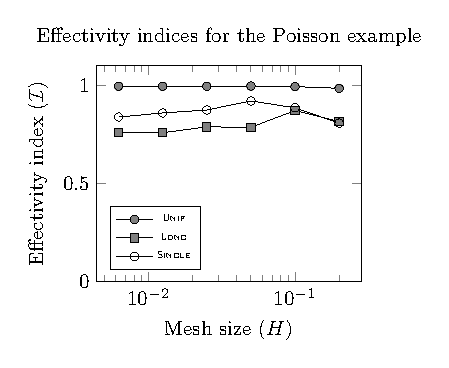
\includegraphics[width=0.5\textwidth]{img/refine_poisson_effectivity}
\caption{Effectivity indices using the Unif,
Long, and Single refinement schemes for
the Poisson example problem}
\label{fig:refine_poisson_effectivity}
\end{figure}

Figure \ref{fig:refine_poisson_effectivity} plots
the effectivity index \eqref{eq:refine_effectivity}
for each of the three schemes at each chosen
mesh size. Effectivity indices for the
baseline \textsc{Unif} method approach
$1$ in the limit as $H \to 0$ as expected. The effectivity
indices obtained using the two non-uniform refinement approaches,
\textsc{Long} and \textsc{Single}, are less accurate
and do not appear to be asymptotically correct.
This is perhaps not surprising, as we have considered a bulk
average for the ratio $\frac{h}{H}$ for these two schemes,
as shown in Table \ref{tab:refine_poisson_ratios}.

%
%% refine_poisson_ratios
\begin{table}[ht!]
\centering
\begin{tabular}{ | c | c | c | } \hline
$H$ & \textsc{Long} : $\frac{h}{H}$ & \textsc{Single} : $\frac{h}{H}$ \\ \hline \hline
$\frac{1}{5}$ & 0.6344 & 0.8198 \\ \hline
$\frac{1}{10}$ & 0.6323 & 0.8212 \\ \hline
$\frac{1}{20}$ & 0.6325 & 0.8204 \\ \hline
$\frac{1}{40}$ & 0.6490 & 0.8183 \\ \hline
$\frac{1}{80}$ & 0.6477 & 0.8202 \\ \hline
$\frac{1}{160}$ & 0.6467 & 0.8195 \\ \hline
\end{tabular}
\caption{Approximated mesh size ratios for the Long and
Single schemes for the first Poisson's equation example.}
\label{tab:refine_poisson_ratios}
\end{table}

However, even though the error estimates themselves obtained by
the \textsc{Long} and \textsc{Single} schemes may not be suitable
for application purposes, these schemes may still be suitable to
drive mesh adaptation at a cheaper cost than the full \textsc{Unif}
approach. For instance, Figure \ref{fig:refine_poisson_dofs}
demonstrates the decrease in the total number of degrees of
freedom for the adjoint problem for the \textsc{Long} and \textsc{Single}
schemes as compared to the \textsc{Unif} scheme. This motivates
us to consider an adaptive example for Poisson's equation in the
next section.

%
%% refine_poisson_dofs
\begin{figure}[ht!]
\centering
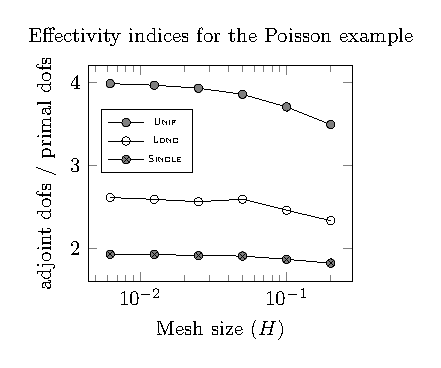
\includegraphics[width=0.5\textwidth]{img/refine_poisson_dofs}
\caption{Ratio of adjoint problem degrees of freedom to primal
problem degrees of freedom using the Unif,
Long, and Single refinement schemes
for the Poisson example problem}
\label{fig:refine_poisson_dofs}
\end{figure}

%%% Mesh Adaptation for Poisson's Equation
\subsection{Mesh Adaptation for Poisson's Equation}

In this example, we again consider the governing equations for Poisson's
equation, as given in the previous section. However, we now choose the
forcing function $f$ to be $f=1$ and the domain
$\Omega := [-1,1] \times [-1,1] \setminus
[-\frac12, \frac12] \times [\frac12, \frac12]$. Further, we consider
the point-wise quantity of interest
$J(u) = \int_{\Omega} \delta(\bs{x} - \bs{x}_0) u \, \text{d} \Omega$,
where the point of interest is chosen to be
$\bs{x}_0 = (0.75, 0.75)$. We again expect the functional to converge
at the rate $k = 2$. The domain and point-wise QoI location are show
in Figure \ref{fig:refine_poisson2_geom}. The value of the quantity
of interest was determined to have a value of $J(u) = 0.0334473
\pm 10e\mbox{-}7$ in the reference \cite{dealiistep14}.

%
%% refine_poisson2_geom
\begin{figure}[ht!]
\centering
\includegraphics[width=0.4\textwidth]{img/refine_squarehole_initial.png}
\caption{Geometry and initial mesh used for the second Poisson's
equation example with the point of interest shown in red.}
\label{fig:refine_poisson2_geom}
\end{figure}

We performed the steps:
\begin{gather*}
\text{Solve Primal} \rightarrow \text{Solve Adjoint} \rightarrow
\text{Estimate Error} \rightarrow \text{Adapt Mesh}
\end{gather*}
7 times, starting from the initial mesh shown in Figure
\ref{fig:refine_poisson2_geom}. We solve the adjoint problem with
three different methods on nested meshes obtained with the
\textsc{Unif}, \textsc{Long}, and \textsc{Single} refinement
schemes. At each adaptive step, the mesh size field was set
according to equation \eqref{eq:refine_size_field}, such that
the target number of elements $N$ is twice that of the current
mesh.

%
%% squarehole_convergence
\begin{figure}[ht!]
\centering
\includegraphics[width=.5\linewidth]{img/refine_squarehole_convergence.pdf}
\caption{Error evolution for adaptive schemes for the second Poisson's equation
example.}
\label{fig:squarehole_convergence}
\end{figure}

Figure \ref{fig:squarehole_convergence} illustrates the convergence
history for the error $J(u) - J(u^H)$ for the three adaptive schemes
obtained with the \textsc{Unif} (Goal Uniform), the \textsc{Long}
(Goal Long), and the \textsc{Single} strategies,
along with the error obtained by solving the primal problem with
successively uniformly refined meshes (Uniform). The rate of
convergence for the \textsc{Unif} scheme agrees with the
reference \cite{dealiistep14}. Additionally, the error for
both the \textsc{Long} and \textsc{Single} schemes converges at a
rate almost near the \textsc{Unif} scheme.

%
%% refine_unif_adapted
\begin{figure}[ht!]
\centering
\begin{subfigure}{.5\textwidth}
\centering
\includegraphics[width=.99\linewidth]{img/refine_squarehole_unif.png}
\end{subfigure}%
\begin{subfigure}{0.5\textwidth}
\centering
\includegraphics[width=.99\linewidth]{img/refine_squarehole_unif_close.png}
\end{subfigure}
\caption{The final adapted mesh using the Unif strategy to
solve the adjoint problem (left) and a close-up of the upper right-hand
corner of this mesh (right).}
\label{fig:refine_unif_adapted}
\end{figure}

Figure \ref{fig:refine_unif_adapted} illustrates the final adapted mesh
obtained using the \textsc{Unif} strategy to solve the adjoint problem.
The distribution of degrees of freedom in this mesh closely resemembles
the results obtained in reference \cite{dealiistep14}. However, using
the \textsc{Long} and \textsc{Single} to solve the adjoint problem
results in final adapted meshes that appear to be largely
unsuitable for application analysis, as shown in Figures
\ref{fig:refine_long_adapted} and
\ref{fig:refine_single_adapted}, even thought these meshes result
in more accurate functional evaluations as compared to uniform
refinement.

%
%% refine_long_adapted
\begin{figure}[ht!]
\centering
\begin{subfigure}{.5\textwidth}
\centering
\includegraphics[width=.99\linewidth]{img/refine_squarehole_long.png}
\end{subfigure}%
\begin{subfigure}{0.5\textwidth}
\centering
\includegraphics[width=.99\linewidth]{img/refine_squarehole_long_close.png}
\end{subfigure}
\caption{The final adapted mesh using the Long strategy to
solve the adjoint problem (left) and a close-up of the upper right-hand
corner of this mesh (right).}
\label{fig:refine_long_adapted}
\end{figure}

%
%% refine_single_adapted
\begin{figure}[ht!]
\centering
\begin{subfigure}{.5\textwidth}
\centering
\includegraphics[width=.99\linewidth]{img/refine_squarehole_single.png}
\end{subfigure}%
\begin{subfigure}{0.5\textwidth}
\centering
\includegraphics[width=.99\linewidth]{img/refine_squarehole_single_close.png}
\end{subfigure}
\caption{The final adapted mesh using the Single strategy to
solve the adjoint problem (left) and a close-up of the upper right-hand
corner of this mesh (right).}
\label{fig:refine_single_adapted}
\end{figure}

%%% CONCLUSIONS
\section{Conclusions and Outlook}

We have developed two alternative approaches to uniform refinement
for performing enriched adjoint solves in adjoint-based error estimation
with two discretization levels. We have applied this approach to
Poisson's equation and demonstrated that. While the number of
degrees of freedom for the adjoint solve for these two
alternative approaches decreases significantly when compared to the
more traditional approach of solving the adjoint problem on
a uniformly refined mesh, the present outlook indicates that
these approaches are not yet suitable for practical applications.
That is, when performing adjoint-based error estimation with the
two novel approaches, effectivity indices are not asymptotically.
Additionally, the meshes obtained with adaptive adjoint-based
analysis display largely qualitatively different features when
compared to the uniform refinement approach.

It is possible that more accurate error estimates could be
obtained by considering the total functional error as the sum
of element-level contributions
\begin{gather}
J^h(u^h) - J^h(u^h_H) \approx \sum_{e=1}^{n_{el}}
- \frac{1}{\alpha_e} \bs{z}^h_e \cdot \bs{R}^h_e(\bs{u}^h_H),
\end{gather}
where we have replaced the approximated ratio
\eqref{eq:refine_ratio} with the exact element-level
ratio, $\alpha_e = 1 - \left( \frac{h_e}{H_e} \right)^k$. Here, the
subscript $e$ denotes the element-level contributions
to the corresponding global quantity. Additionally, it is
possible that more suitable meshes may be obtained during
the adaptive process if some sort of size field smoothing
algorithm is utilized. We leave investigation into these
areas as a suggestion for future work.

\chapter{ALGORITHM SELECTION AND HYPERPARAMETER OPTIMIZATION BASED QUANTIFICATION OF ERROR CONTRIBUTION IN IMAGE CLASSIFICATION PIPELINES}
\label{chap:EP}

\let\thefootnote\relax\footnotetext{
This chapter has been submitted for publication:
A. Chowdhury, M. Magdon-Ismail, H. Su, and B. Yener. ``Algorithm selection and hyperparameter optimization based quantification of error contribution in image classification pipelines." \emph{IEEE International Conference on Data Mining}}
%%%%%%%%%%%%%%%%%%%%%%%%%%%%%%%%%%%%%%%%%%%%%%%%%%%%%%%%%%%%%%%%%%%%%%%%%%%%%%
%\section{Introduction and Motivation}
%%%%%%%%%%%%%%%%%%%%%%%%%%%%%%%%%%%%%%%%%%%%%%%%%%%%%%%%%%%%%%%%%%%%%%%%%%%%%%

\section{Introduction} 
\label{sec1}
In this chapter, we present a methodology to quantify the contributions of different components of an image classification pipeline in terms of the classification error. This is different to the last chapter where we introduced a methodology to quantify the error from the image samples acquired using acquisition techniques like microscopes.
Machine learning and data science has entered many domains of human effort in modern times. The number of self-reported data scientists has doubled in recent years \cite{harrison1995validity}. They have entered various domains including academia, industry and business among others. There has therefore been a demand for machine learning tools that are flexible, powerful and most importantly interpretable. The effective application of machine learning tools unfortunately requires an expert understanding of the frameworks and algorithms that are present in a machine learning pipeline. It also requires knowledge of the problem domain and understanding of the assumptions used in the analysis. In order for these tools to be used adequately by non-experts; additional tools must be developed for understanding and interpreting the results of the application of a data analytic pipeline on a domain specific problem.  

\begin{figure}[ht!]
    \centering
    \includegraphics[scale=0.5]{img/EP/generalized_pipeline}
    \caption{Representation of a machine learning pipeline. This is represented as a generalized directed acyclic graph. $S_i$ represents the $i$-th computational step in the pipeline and $A_{ij}$ represents the $j$-th algorithm in the $i$-th step. $X$ is the input dataset and $Y$ is the evaluation metric.}
    \label{fig:pipeline}
\end{figure}

Pipelines in machine learning and data science are commonly organized in the form of interdependent components. Such components that make up a data analytic pipeline include data preprocessing, feature extraction, feature transformation, model building and model evaluation among others. Such pipelines provide a natural way to organize such tasks, and they play a key part in the design and implementation of large scale data science projects. Machine learning toolboxes like scikit-learn \cite{pedregosa2011scikit}, RapidMiner \cite{mierswa2006yale} and Apache Spark \cite{spark2016apache} independently provide frameworks for implementing pipelines. Fig. \ref{fig:pipeline} shows a generic representation of data analytic pipelines. Each computational step of the pipeline $S_{i}$ consists of several algorithms ($A_{ij}$) to choose from. Each algorithm in the pipeline consists of its own hyperparameters $\theta_{ijk}$ that must be optimized for using the algorithm. Therefore, there are an exponential number of combinations of algorithms and hyperparameters in a given analytic pipeline skeleton. This then is an extremely computationally intensive task of optimizing the pipeline. Tuning this pipeline can be viewed as the optimization of an objective function that is noisy and expensive to evaluate. The input to the pipeline is the input dataset $X$, the pipeline $P$(consisting of the steps $S_{i}$, the algorithms $A_{ij}$ and corresponding hyperparameters $\theta_{ijk}$) and the output performance $Y$ such as validation error, accuracy, F1-score and cross-entropy loss among others, which are examples of the objective function.The goal of a data scientist is to find the best set of algorithms and hyperparameters in this pipeline that optimizes the objective function. This corresponds to finding an optimal path through the pipeline in Fig. \ref{fig:pipeline}.  Simple methods such as grid and random search \cite{bergstra2012random} have been used to tackle this problem. More complicated approaches such as Bayesian optimization \cite{snoek2012practical, zhang2016flash} have been used successfully for approaching more difficult problems. Pipeline optimization as a whole has also been approached using genetic algorithms \cite{olson2016evaluation, olson2016tpot, olson2016automating}.
We use grid search, random search and bayesian optimization methods for optimization of the pipeline and each individual path in it.  

Interpretation of machine learning pipelines is extremely important for their adoption in various domains. Domain experts prefer to understand how predictive decisions are made by the pipeline. Recently there has been an advent of models and techniques for improving the interpretability of machine learning. \cite{ribeiro2016model} introduces a model-agnostic method for interpreting the results complex machine learning algorithms. \cite{doshi2017towards} attempts at a definition of interpretability in this context and how it should be measured. \cite{koh2017understanding} uses influence functions to understand blackbox predictions. In this work, we attempt to provide an interpretation of machine learning pipelines in terms of the importance and sensitivity of components in the pipeline (steps, algorithms and hyperparameters) as opposed to the approaches which are geared toward interpretation of algorithms based on the dataset like \cite{koh2017understanding}. This includes understanding the predictions with respect to components of steps like feature extraction and feature transformation and also smaller components like individual hyperparameters. To our knowledge, this type of approach to interpretation has not been taken before.
To this end, we propose the understanding of the contribution of error in data analytic pipelines. We use the cross-entropy loss as the performance metric of the optimization algorithms and basis of error quantification in the image classification pipelines. Understanding the importance of the components in the predictive model is important for experts to design the data analytic pipelines. Experts can use the information from error contributions to focus attention on certain parts of the pipeline depending on the source of error. In addition, it also provides non-experts in machine learning insight into the predictions of the model. They can understand whether the error they are seeing are due to which component of the process. We introduce a methodology to quantify the contribution of error from different components of the data analytic pipeline, namely the computational steps and algorithms in the pipeline. 
% In addition, a model of error propagation is proposed in this work. This model represents the propagation of error from the computational steps in the pipeline starting from the first step that could be data preprocessing in Fig. 1 to the last step that is usually learning algorithms in a machine learning problem.  

Pipeline optimization methods and algorithms like grid search, random search \cite{bergstra2012random} and Bayesian optimization \cite{snoek2012practical} are used to optimize the pipeline for performing experiments with the error quantification methodology. We take two different approaches to optimization. The first is hyper-parameter optimization (HPO) where a computational path in Fig. \ref{fig:pipeline} is optimized. This is equivalent to a combined optimization of the hyperparameters of the algorithms on that path. The second type of optimization is denoted as combined algorithm selection and hyperparameter optimization (CASH). This term was introduced in \cite{thornton2013auto}. This is a more difficult problem, because the pipeline is optimized globally, in that the result of the optimization is a single optimized path that produces the best performance over all the paths in the machine learning workflow.  

We use four datasets to demonstrate the error quantification methodology. The machine learning problem is that of image classification. We show the performance of both the optimization frameworks (HPO and CASH) for the experiments. We show experimentally that CASH using random search can be efficiently used for quantification of errors from the different computational steps of the pipeline. In addition, HPO frameworks of both Bayesian optimization and random search provides  estimates of error contributions from the algorithms and hyperparameters in a particular path of the pipeline.
% We use the computationally efficient CASH framework of random search to perform experiments on the error propagation model. 
We demonstrate from the results that the error quantification methodology maybe used by both data science and domain experts to improve and interpret the results of image classification pipelines.  

The paper is organized as follows. Section \ref{sec2} describes the methods that are used in this work and the proposed methodology of error contribution. The experimental frameworks, datasets, results and discussion makes up section \ref{sec3}. This is followed by the conclusion in section \ref{sec4}.

\section{Foundations}
\label{sec2}
In this section we describe the optimization problem and methods that are used in this work. 
\subsection{Algorithm selection and hyper-parameter optimization}
\label{subsec_AS_HPO}
We approach the problem of optimization of the pipeline from two frameworks. In one framework, each path in the pipeline in Fig. \ref{fig:pipeline} is individually optimized. This essentially boils down to problem of hyper-parameter optimization (HPO)  because the hyperparameters of each algorithm are optimized for each individual path. In the second framework, the entire pipeline is optimized. This means that the algorithms and hyperparameters are optimized together. This is denoted as combined algorithm selection and hyper-parameter optimization (CASH).

\subsubsection{Hyper-parameter optimization (HPO)}
\label{subsubsec_HPO}
Let the \textit{n} hyperparameters in a path be denoted as $\theta_1, \theta_2, ..., \theta_n$, and let $\Theta_1, \Theta_2, ..., \Theta_n$ be their respective domains. The hyperparameter space of the path is  \textbf{$\Theta$} = $\Theta_1 \times \Theta_2 \times ... \times \Theta_n$.


When trained with $\emph{$\theta$} \in \textbf{$\Theta$}$ on data $D_{train}$, the validation error is denoted as \par
\noindent $\mathcal{L}(\theta, D_{train}, D_{valid})$. Using $k$-fold cross-validation, the hyperparameter optimization problem for a dataset $D$ is to minimize:
\begin{equation}
f^D(\theta) = \frac{1}{k}\sum_{i=1}^{k} \mathcal{L}(\emph{$\theta$}, D_{train}^{(i)}, D_{valid}^{(i)})
\label{eq:hpo}
\end{equation}
Hyperparameters $\theta_i$ may be numerical, categorical or conditional with a finite domain. The minimization of this objective function provides the optimal configuration of hyperparameters on a particular path in the pipeline in Fig. \ref{fig:pipeline}. The optimization of the objective function defined by Eq. \ref{eq:hpo} is very expensive. Depending on the type of hyper-parameter variables, the derivatives and convexity properties maybe unknown, and derivative free global optimization methods like Bayesian optimization and techniques like random search maybe used to tackle this problem.

\begin{figure}[ht!]
    \centering
    \includegraphics[scale=0.4]{img/EP/HPO}
    \caption{Hyper-parameter optimization in a data analytic pipeline. Each path in the pipeline is individually optimized.}
    \label{fig:HPO}
\end{figure}

\subsubsection{Combined algorithm selection and hyper-parameter optimization (CASH)}
\label{subsubsec_CASH}
We can define the CASH formulation using Fig. 1. Let there be $n$ computational steps in the pipeline. Each step $i$ in the pipeline consists of algorithms $A_i(\Theta_i)$, where $A_i(\Theta_i) = \{A_{i1}(\theta_{i1}), ..., A_{im_{i}}(\theta_{im_{i}})\}$, $m_{i}$ is the number of algorithms in step $i$, $A_{ij}$ represents the $j$-th algorithm in step $i$, and \textbf{$\theta_{ij}$} represents the set of hyperparameters corresponding to  $A_{ij}$. The entire space of algorithms and hyperparameters is therefore given by \par
\noindent $\mathcal{A} = A_1(\Theta_1) \times A_2(\Theta_2) \times ... \times A_n(\Theta_n)$. The objective function to be minimized for CASH is given by
\begin{equation}
f^D(A) = \frac{1}{k}\sum_{i=1}^{k} \mathcal{L}(\emph{A}, D_{train}^{(i)}, D_{valid}^{(i)}) 
\label{eq:cash}
\end{equation}
where, $A \in \mathcal{A}$ and other notations are the same as those introduced in the previous section.
Similar to the objective function defined over the hyperparameters in Eq. \ref{eq:hpo}, the optimization in Eq. \ref{eq:cash} is even more difficult due to the additional problem of algorithm selection. Again, the derivates may be impossible to compute and convexity properties may be completely unknown.

\begin{figure}[ht!]
    \centering
    \includegraphics[scale=0.4]{img/EP/CASH}
    \caption{Combined algorithm selection and hyper-parameter optimization in a data analytic pipeline. The algorithms and corresponding hyperparameters are optimized simultaneously.}
    \label{fig:CASH}
\end{figure}


\subsection{Optimization methods}
\label{optimization}
The critical step in HPO or CASH is to choose the set of trials in the search space, which is $\Theta$ for HPO and $\mathcal{A}$ for CASH. In this section, methods that are used in this paper for optimization of Eq. \ref{eq:hpo} and Eq. \ref{eq:cash} are described. Grid search, random search and Bayesian optimization are used in this work.
\subsubsection{Grid search}
\label{grid}
Grid search is the simplest of all methods for coming up with trials in the search space. The set of trials in grid search is formed by assembling every possible set of values in $\Theta$ (HPO) and $\mathcal{A}$ (CASH) and computing the validation loss for each. The configuration $\theta \in \Theta$ or $A \in \mathcal{A}$ that minimizes the validation loss $\mathcal{L}$ is chosen as the optimum configuration. Unfortunately grid search is computationally very expensive. For HPO, the number of trials corresponds to $\prod_{i=1}^n |\Theta_i|$, and for CASH this is $\prod_{i=1}^n |A_i(\Theta_i)|$. This product makes grid search suffer from the \textit{curse of dimensionality}. This is because the number of trials grows exponentially with the number of hyperparameters. However, grid search has certain advantages. Firstly, parallelization and implementation is trivial. In addition, grid search is robust in the sense that results maybe replicated easily. 

\subsubsection{Random search}
\label{random}
Random search is the optimization method where trial configurations are randomly sampled from the search space of $\Theta$ (HPO) or $\mathcal{A}$ (CASH). \cite{bergstra2012random} shows empirically and theoretically that randomly selecting trials is sufficiently accurate and more efficient than performing optimization using grid search. We also show similar results in this work.

\subsubsection{Bayesian optimization}
\label{bayesian}
Sequential model based Bayesian optimization (SMBO) \cite{hutter2011sequential} is the method of choice when it comes to optimization of complicated black-box functions. In a nutshell, it consists of two components. The first is a probabilistic model and the second is an acquisition function. The probabilistic model can be modelled using Gaussian processes (Spearmint) \cite{snoek2012practical}, random forests (SMAC) \cite{hutter2011sequential} and using density estimation with Tree-structured Parzen estimators (TPE) \cite{bergstra2011algorithms}. The acquisition function determines the future candidates or trials for evaluation. The acquisiton function is relatively cheap to evaluate compared to the actual objective function $f^D$. One of the most prominent acquisition functions is \textit{expected improvement} (EI) \cite{expected_improvement}. We use the sequential model-based algorithm configuration (SMAC) that uses random forests as the Bayesian optimization framework. This is because it can be used for optimizing conditional hyperparameter configurations. The choice is also based on empirical results in \cite{eggensperger2013towards}.

\section{Proposed methods}
\label{sec3}
In this section the proposed methodology for quantification of error contribution is presented. The method is independent of the optimization methods that maybe used for both the HPO and CASH formulations.

\subsection{Error contribution with the agnostic methodology}
\label{EQ}
Machine learning pipelines maybe understood and interpreted by quantifying the contribution of error from different parts of the pipeline. For example, it is useful for machine learning experts and domain experts to understand and identify where the source of the error is in a pipeline. Referring back to Fig. \ref{fig:pipeline}, if it was known that most of the error in the final result originated from feature extraction, then machine learning practitioners would devote more time and energy to coming up with better algorithms for feature extraction or fine-tuning the algorithms in that step to reduce the error. In addition, if it were possible to quantify the contribution of errors from certain algorithms or hyperparameters in the pipeline, then the data scientists would try to fine tune the algorithms in the pipeline or even try to replace the algorithms with better alternatives. 

We propose an \textit{agnostic} methodology for quantifying error contributions from different parts of the pipeline. It is quantified as the minimum error obtained by being agnostic to a particular component of the pipeline (computational step, algorithms or hyperparameters). We shall define what \textit{agnostic} refers to for both computational steps, algorithms and hyperparameters individually.

\subsubsection{Quantification of error from computational steps}
\label{subsubsec_eq_steps}
The \textit{agnostic} methodology maybe used for quantification of contributions from computational steps like feature extraction, data pre-processing and learning algorithms. Being \textit{agnostic} to a computational step means that the algorithms in that step are selected randomly for that step while the remaining pipeline is optimized. The average of the minimum errors obtained with each algorithm in the step used as the only algorithm in that particular step, provides an estimate of the agnostic error from a particular pipeline.  
More formally, the agnostic methodology is implemented for computational steps in the following manner. Using Fig. \ref{fig:pipeline} as a reference, let $n$ be the number of steps in the pipeline. Each step in the pipeline is denoted as $S_i$. $|S_i|$ is the number of algorithms in step $i$. $A_{ij}$ denotes the $j$-th algorithm in the $i$-th step. $E^*$ represents the minimum validation error found after optimization of the entire pipeline (using the CASH framework). $E_{A_{ij}}^*$ is the minimum  validation error found with $A_{ij}$ as the only algorithm in step $i$. The error contribution from step $i$, $EC_{S_i}^*$ is given by Eq. \ref{eq_step}.
\begin{equation}
\label{eq_step}
EC_{S_i}^* = \frac{1}{|S_i|}\sum_{z=1}^{|S_i|} E_{A_{ij}}^* - E^*,
\end{equation}
where, $i = {1, ..., n}, j = {1, ..., |S_i|}$
Taking the difference with respect to the global minimum in Eq. \ref{eq_step} provides an estimate of the error contribution from step $i$ of the pipeline. A large value of $EC_{S_i}^*$ would mean that step $S_i$ is important for the pipeline.

\subsubsection{Quantification of error from algorithms}
\label{subsubsec_eq_alg}
The \textit{agnostic} methodology for algorithms is implemented as follows. Similar to the \textit{agnostic} methodology for steps, we define the \textit{agnostic} methodology for algorithms. In this case, we focus on a single path in the pipeline in Fig. 1. Let's assume we are trying to quantify the error contribution of a particular algorithm $A_{ij}$ that lies on path $p$. Being $agnostic$ to $A_{ij}$ means we optimize everything else on the path except the algorithm. This means that we pick the hyperparameters $\theta_{ij}$ of algorithm $A_{ij}$ randomly while optimizing the rest of the algorithms on the path. This is formally calculated by taking the average of the optimum errors on the path for each configuration of $\theta_{ij}$. The minimum validation error on the path is then subtracted from this error to give us the error contribution from algorithm $A_{ij}$ on path $p$. These errors are computed using the results and the search trials on the CASH framework in section \ref{subsubsec_CASH}.

\begin{equation}
\label{eq_alg}
EC_{A_{ij}}^* = \frac{1}{|\theta_{ij}|}\sum_{z=1}^{|\theta_{ij}|} {E_{A_{ij}}^z}^* - {E_{A_{ij}^p}^*},
\end{equation}

where, $i = {1, ..., n}, j = {1, ..., |\theta_{ij}|}$, $|\theta_{ij}|$ represents the number of hyperparametric configurations of $A_{ij}$,  ${E_{A_{ij}}^z}^*$ is the minimum error obtained with the $z$-th configuration of $\theta_{ij}$ and $E_{A_{ij}^p}^*$ is the minimum error found over the path $p$ that consists of algorithm $A_{ij}$.


\subsubsection{Quantification of error from hyperparameters}
\label{subsubsec_eq_hyper}
The \textit{agnostic} methodology for hyperparameters is implemented as follows. In the case of hyperparameters, we focus on a single path similar to what we did for algorithms. Let's assume we are trying to quantify the error contribution of a particular hyper-parameter $\theta_{ijk}$ that lies on path $p$, i.e. the $k$-th hyper-parameter of the $j$-th algorithm in the $i$-th step of the pipeline. Being $agnostic$ to $\theta_{ijk}$ means we optimize everything else on the path except the hyper-parameter. This means that we pick the hyperparameter $\theta_{ijk}$ of algorithm $A_{ij}$ randomly while optimizing the rest of the hyperparameters on the path. This is formally calculated by taking the average of the optimum errors on the path for each configuration of $\theta_{ijk}$. The minimum validation error on the path is then subtracted from this error to give us the error contribution from hyper-parameter $\theta_{ijk}$ on path $p$. This is again computed using the HPO framework described in section \ref{subsubsec_HPO}.

\begin{equation}
\label{eq_hyper}
EC_{\theta_{ijk}}^* = \frac{1}{|\theta_{ijk}|}\sum_{z=1}^{|\theta_{ijk}|} {E_{\theta_{ijk}}^z}^* - {E_{A_{ij}^p}^*},
\end{equation}

where, $i = {1, ..., n}, j = {1, ..., |\theta_{ij}|}$, k = number of hyperparameters of algorithm $A_{ij}$. $|\theta_{ijk}|$ represents the number of configurations of $\theta_{ijk}$,  ${E_{\theta_{ijk}}^z}^*$ is the minimum error obtained with the $z$-th configuration of $\theta_{ijk}$ and $E_{A_{ij}^p}^*$ is the minimum error found over the path $p$ that consists of algorithm $A_{ij}$.


\section{Experiments and results}
\label{sec4}
In this section, we describe the experiments performed on the data analytic pipeline to quantify the error contributions from different components of the pipeline. Image classification is the data analytic problem chosen for demonstrating the error quantification experiments. A representation of an image classification pipeline is shown in Fig. \ref{fig:flowchart} in the form of a flowchart.  
\begin{figure}[ht!]
    \centering
    \includegraphics[scale=0.4]{img/EP/flowchart}
    \caption{Representation of an image classification pipeline. The pipeline consists of the steps represented by green ellipses and the outputs of each step represented by blue rectangles. In this work, we focus on the steps and outputs after pre-processing.}
    \label{fig:flowchart}
\end{figure}
In this work, we focus on real world scientific datasets from the domains of medical pathology and material science.  Therefore, the flowchart starts with a sample that is imaged with acquisition technology like a camera or a microscope. The image is then processed using image pre-processing algorithms like normalization and standardization. This may also include image segmentation algorithms. This is followed by feature extraction algorithms that extract useful information from the images. Sometimes, the features extracted are transformed to a different vector space using feature transformation (feature selection or dimensionality reduction) algorithms. The dataset is then divided into training and test datasets in a 80-20 split. Finally, classification algorithms like random forests \cite{breiman2001random} and support vector machines (SVM) \cite{cortes1995support} are used for learning in order to build a predictive model for the image classification problem. The performance of the pipeline is evaluated using classification metrics like F1-score, accuracy, precision and recall. We use the cross entropy loss on the validation data as the estimate of the out-of-sample error. This error is then used as a feedback to quantify the contribution of the errors from different components of the pipeline. The specific pipeline used in this work is shown in the following figure.

\begin{figure}[ht!]
    \centering
    \includegraphics[scale=0.3]{img/EP/pipeline}
    \caption{Representation of the image classification pipeline as a directed acyclic graph used in this work. This is an instantiation of the generalized data analytic pipeline in Fig. \ref{fig:pipeline}}
    \label{fig:images_pipeline}
\end{figure}

 The above figure shows the pipeline used in this work. There are 3 computational steps in this pipeline, namely feature extraction ($S_1$), feature transformation ($S_2$) and learning algorithms ($S_3$). The steps, algorithms and corresponding hyperparameters $A_{ij}(\theta_{ij})$ is described in Table \ref{table:algorithms_table}.

\begin{table}[ht!]
\centering
\caption{Algorithms and hyperparameters used in the image classification pipeline. The specific algorithms and corresponding \textit{hyperparameters} are defined in the last column}
\begin{tabular}{@{} |m{9.7em}|m{1.5cm}|m{8cm}| @{}} 
 \hline
 Step & $A_{ij}(\theta_{ij})$ & Definition \\ 
 \hline
 \multirow{3}{*}{Feature extraction} & $A_{11}(\theta_{11})$ & Haralick texture features (\textit{Haralick distance}) \\ 
 & $A_{12}(\theta_{12})$ & Pre-trained CNN trained on ImageNet \cite{deng2009imagenet} database with VGG16 \cite{simonyan2014very} network  \\
  & $A_{13}(\theta_{13})$ & Pre-trained CNN trained on ImageNet \cite{deng2009imagenet} database with Inception \cite{szegedy2016rethinking} network  \\
 \hline
 \multirow{3}{*}{Feature transformation} & $A_{21}(\theta_{21})$ & PCA ($whitening$) \cite{wold1987principal} \\
 & $A_{22}(\theta_{22})$ & ISOMAP (\textit{number of neighbors, number of components}) \cite{tenenbaum2000global} \\
 \hline
 \multirow{3}{*}{Learning algorithms} & $A_{31}(\theta_{31})$ & Random forests (\textit{number of trees, maximum features}) \cite{breiman2001random} \\
 & $A_{32}(\theta_{32})$ & SVM ($C, \gamma$) \cite{cortes1995support}\\
 \hline
 \end{tabular}
 \label{table:algorithms_table}
\end{table}
The algorithms defined in the table are selected for making up the components of the pipeline in Fig. \ref{fig:images_pipeline}. This is meant to serve as an example for demonstrating the experiments using the error contribution framework described in section \ref{sec3}. It can easily be generalized to any data analytic problem that involve pipelines. 

\subsection{Optimization frameworks}
\label{frameworks}
Experiments are performed using two optimization frameworks. These frameworks have been described in detail in Section \ref{subsec_AS_HPO}. 
The first global optimization framework is the CASH framework described in Section \ref{subsubsec_CASH}. Here, the pipeline is optimized as a whole including the algorithms, which are themselves considered as hyperparameters in this framework. The following figure is a representation of this. This is used for quantification of the contribution of error with respect to \textit{computational steps} in the pipeline.

The second framework is the hyperparameter optimization (HPO) framework where each path in the pipeline is optimized individually. This is described in detail in section \ref{subsubsec_HPO}. This framework is used for quantifying the contribution of error with respect to algorithms and hyperparameters in the each path of the pipeline.

Specifically, we choose the path \textit{haralick texture features} - \textit{PCA} - \textit{random forests} to demonstrate the error quantification approach for algorithms and hyperparameters.

\subsection{Datasets}
Four datasets from the domains of medicine and material science are used in this work. They are image datasets of breast cancer\cite{bilgin2007cell}, brain cancer \cite{gunduz2004cell}, and two datasets of microstructures in material science \cite{chowdhury2016image}. They are described in the following table.

\begin{table}[ht!]
\centering
\caption{Descriptions of the datasets used in this work}
\begin{tabular}{ |c|c| } 
 \hline
 Dataset (notation) & Distribution of classes \\ 
 \hline
 Breast cancer (\textit{breast}) \cite{bilgin2007cell} & \textit{benign}: 151, \textit{in-situ}: 93, \textit{invasive}: 202\\
 \hline
 Brain cancer (\textit{brain}) \cite{gunduz2004cell} & \textit{glioma}: 16, \textit{healthy}: 210, \textit{inflammation}: 107\\
 \hline
  Material science 1 (\textit{matsc1}) \cite{chowdhury2016image} & \textit{dendrites}: 441, \textit{non-dendrites}: 132 \\
 \hline
 Material science 2 (\textit{matsc2}) \cite{chowdhury2016image} & \textit{transverse}: 393, \textit{longitudinal}: 48 \\
 \hline
 \end{tabular}
\label{table:datasets}
\end{table}
The above table represents datasets from the scientific domain. These datasets have been chosen because they represent examples of real world datasets. They are noisy in the sense that they have artefacts in the images, are heavily imbalanced and are small in terms of number of samples. They are different from the very large datasets like ImageNet \cite{deng2009imagenet}, where deep learning techniques like convolutional neural networks have been shown to be superior. Even though deep neural networks represent an end-to-end workflow where the input image is fed into the network and the output classification is obtained at the other end, they may also be represented as pipelines, if the hyperparameters of the network are considered. \cite{shin2016deep} has shown that machine learning problems involving datasets from medical imaging may be solved using pre-trained and fine-tuned neural networks rather than training them from scratch. We have therefore used pre-trained models such as VGGnet \cite{simonyan2014very} and InceptionNet \cite{szegedy2016rethinking} as pre-trained feature extraction models that fit naturally in the pipeline framework described here for the purpose of illustrating the error quantification methodology.




\subsection{Error quantification experiments}
\label{eq_expts}
Experiments based on the quantification of error contributions framework described in section \ref{EQ} are presented here. The plots are of the error contribution values calculated using Eqs. \ref{eq_step}, \ref{eq_alg} and \ref{fig:eq_hyper} on the 4 datasets described in Table \ref{table:datasets}. 
\subsubsection{Experimental setting}
Optimization using the 3 algorithms in section \ref{optimization} is performed using the pipeline in Fig. \ref{fig:images_pipeline} on the 4 datasets in Table \ref{table:datasets}. The domain and possible values of the hyperparameters are described in the following table. 
The convergence criteria (a hyper-hyper-parameter) is set at 50 iterations of unchanging  function value for each of the optimization methods. The choice of the convergence criteria and hyperparameters are independent of the error quantification methods. Results maybe obtained by using any choice of values for these components. The continuous hyperparameters \textit{maximum features}, \textit{C} and $\gamma$ have been described specifically for comparison of the optimization methods with grid search. In general, discretization of the hyperparameters is not necessary for performing optimization.
\begin{table}[ht!]
\centering
\caption{Hyper-parameter domains corresponding the algorithms in Table \ref{table:algorithms_table} used by the optimization methods}
\begin{tabularx}{\linewidth}{ |X|X|X|X| } 
 \hline
 Algorithm & Hyper-parameter & Description & Values \\ 
 \hline
 Haralick texture feature & \textit{Haralick distance} & The Haralick distance to consider while computing the co-occurence matrix & [1, 2, 3, 4]\\
 \hline
 PCA & \textit{whitening} & Flag variable for whitening the data & [True, False]\\
 \hline
  ISOMAP & \textit{number of neighbors} & Number of neighbors to consider for each point & [3, 4, 5, 6, 7] \\
 \hline
 ISOMAP & \textit{number of components} & Number of co-ordinates for the manifold in ISOMAP algorithm & [2, 3, 4]\\
 \hline
 Random forests & \textit{number of estimators} & Number of trees in the forest & [8,  81, 154, 227, 300]\\
 \hline
 Random forests & \textit{maximum features} & The fraction of the total number of features to consider when looking for the best split & [0.3, 0.5, 0.7]\\
 \hline
 SVM & \textit{C} & Penalty parameter of the error term & [0.1, 25.075, 50.05, 75.025, 100.0] \\
 \hline
 SVM & $\gamma$ & Kernel coefficient for the radial basis function & [0.3, 0.5, 0.7] \\
 \hline
 \end{tabularx}
 
\label{table:hyper}
\end{table}
The error contribution values are obtained from the trials in the optimization methods described in Section \ref{sec2}. Grid search is only run once while the other algorithms are averaged over 5 runs with the mean and standard deviation shown in the following plots. These results are computed on the validation error (cross-entropy loss) obtained at the end of the pipeline. Random search and Bayesian optimization (using the SMAC algorithm) are implemented on both the frameworks described in Section \ref{frameworks}. The grid search results maybe used as the gold standard to compare the performance of other optimization algorithms. 

\subsubsection{Error contribution from computational steps}
The mean and standard deviation values of $EC_{S_i}$ calculated using Eq. \ref{eq_step} is represented in Fig. \ref{fig:eq_steps} for the 4 datasets in Table \ref{table:datasets}. The error is calculated using the formulation of $EC_{S_i}$ in section \ref{subsubsec_eq_steps}. We observe that most of the contribution comes from feature extraction algorithms. This means that it is most important to optimize the feature extraction step among the other steps as it is of most importance based on the plots. This confirms our intuitive belief that feature extraction algorithms are the most important components of a machine learning pipeline. 
\begin{figure}[ht!]
\centering
\begin{subfigure}{.5\textwidth}
  \centering
  \includegraphics[scale=0.37]{img/EP/agnostic_error_steps_breast.eps}
  \caption{\textit{breast}}
  \label{fig:eq_steps_breast}
\end{subfigure}%
\begin{subfigure}{.5\textwidth}
  \centering
  \includegraphics[scale=0.37]{img/EP/agnostic_error_steps_brain.eps}
  \caption{\textit{brain}}
  \label{fig:eq_step_brain}
\end{subfigure}
\begin{subfigure}{.5\textwidth}
  \centering
  \includegraphics[scale=0.37]{img/EP/agnostic_error_steps_matsc_dataset1.eps}
  \caption{\textit{matsc1}}
  \label{fig:eq_steps_matsc1}
\end{subfigure}%
\begin{subfigure}{.5\textwidth}
  \centering
  \includegraphics[scale=0.37]{img/EP/agnostic_error_steps_matsc_dataset2.eps}
  \caption{\textit{matsc2}}
  \label{fig:eq_steps_matsc2}
\end{subfigure}
\caption{Plots of error contributions from computational steps in the pipeline. The x-axis represents the steps in the pipeline - feature extraction, feature transformation and learning algorithms. The y-axis shows the values of the contributions from the corresponding steps in the pipeline. The maximum contribution in terms of error is from the feature extraction step in the pipeline. Random search (blue) follows the behavior of grid search (red) more accurately than Bayesian optimization (yellow). Hence, random search maybe used to quantify the error contributions instead of grid search.}
\label{fig:eq_steps}
\end{figure}

Let us look at Fig. \ref{fig:eq_steps_breast} (contribution of the steps on the \textit{breast}) as an example. Here we see that the contribution from the steps reduces in magnitude as we move towards the end of the pipeline. This trend is quantified by all of the three methods - grid search, random search and Bayesian optimization. However, Bayesian optimization is not able to capture the contribution from feature transformation as accurately as random search with respect to grid search.
 The standard deviation of grid search is 0 because it was only run once for each dataset due to the time required for computation and also because of the robustness of the grid search method (the results don't change because we try out every single configuration). We observe from the results, that random search follows the behavior of grid search. It mirrors the behavior of grid search, but the results are not robust because of the high standard deviation. This is expected because the search trials may not include all the configurations in the pipeline as opposed to grid search where all the configurations of algorithms and hyperparameters are evaluated. The results of SMAC (bayesian optimization) in the CASH framework do not follow the behavior of grid search as closely as random search. This is because the trials for SMAC are even more sparse with respect to the algorithms it selects for optimization of  the error in Eq. \ref{eq_step}. SMAC only samples a few configurations based on the updated probabilistic model as it narrows in on the optimum configuration. Therefore, it sometimes gives erroneous results as can be seen by the contribution of feature transformation in Fig. \ref{fig:eq_steps}.


\subsubsection{Error contribution from algorithms}

% In the following figure, the error contributions from algorithms are quantified using theformulation in Section 3.1.2.  This is represented asmethod1 in the experiments.  As men-tioned before, we see that only 3 algorithms corresponding to the each step in the pipelinethat lie on the best path are dominant in terms of error contribution.
In the following figure, the error contributions from algorithms are quantified using the formulation in Section \ref{subsubsec_eq_alg}. We select \textit{haralick texture features}, $PCA$ and \textit{random forests} as the path to demonstrate the contribution of error from algorithms, because each of these algorithms are associated with one or more hyperparameters. We observe a trend here, in that, the contribution from \textit{haralick texture features} and \textit{random forests} is more than $PCA$. This means that it is more important to tune \textit{haralick texture features}, and \textit{random forests} than it is to tune  $PCA$. This maybe attributed to the fact that the search space of hyperparameters (in Table \ref{table:hyper}) for \textit{haralick texture features} and \textit{random forests} is larger than that of \textit{PCA}. Again, we see the trend that random search performs better and is more robust in terms of following the behavior of grid search than Bayesian optimization.

% This issue is redressed by the second  formulation for error contribution from algorithms in 3.1.2 which is shown in Fig. 9.
\begin{figure}[ht!]
\centering
\begin{subfigure}{.5\textwidth}
  \centering
  \includegraphics[scale=0.37]{img/EP/agnostic_error_alg_breast.eps}
  \caption{\textit{breast}}
  \label{fig:eq_alg_breast}
\end{subfigure}%
\begin{subfigure}{.5\textwidth}
  \centering
  \includegraphics[scale=0.37]{img/EP/agnostic_error_alg_brain.eps}
  \caption{\textit{brain}}
  \label{fig:eq_alg_brain}
\end{subfigure}
\begin{subfigure}{.5\textwidth}
  \centering
  \includegraphics[scale=0.37]{img/EP/agnostic_error_alg_matsc_dataset1.eps}
  \caption{\textit{matsc1}}
  \label{fig:eq_alg_matsc1}
\end{subfigure}%
\begin{subfigure}{.5\textwidth}
  \centering
  \includegraphics[scale=0.37]{img/EP/agnostic_error_alg_matsc_dataset2.eps}
  \caption{\textit{matsc2}}
  \label{fig:eq_alg_matsc2}
\end{subfigure}

\caption{Plots of error contributions from algorithms in the pipeline. The x-axis represents the algorithms in the path - \textit{haralick texture features}, $PCA$ and \textit{random forests}. The y-axis shows the values of the contributions from the corresponding algorithms in the path. Random search again mirrors the trend of grid search more than bayesian optimization. Therefore random search maybe used instead of grid search for computing the contribution of error from algorithms in a path. The plots also show that it is more important to tune \textit{haralick texture features}, and \textit{random forests} than it is to tune  $PCA$. }
\label{fig:eq_alg}
\end{figure}
Let us take the example of the error contribution of algorithms over the selected path in the \textit{brain} dataset depicted in Fig. \ref{fig:eq_alg_brain}. We observe that \textit{random forests} has the most amount of contribution with respect to the error followed by \textit{haralick texture features} and \textit{PCA} respectively. Again we see that Bayesian optimization is not able to capture the error contributions from \textit{random forests} adequately.

\subsubsection{Error contribution from hyperparameters}

% In the following figure, the error contributions from algorithms are quantified using theformulation in Section 3.1.2.  This is represented asmethod1 in the experiments.  As men-tioned before, we see that only 3 algorithms corresponding to the each step in the pipelinethat lie on the best path are dominant in terms of error contribution.
Fig. \ref{fig:eq_hyper} shows the error contributions from hyperparameters quantified using the formulation in Section \ref{subsubsec_eq_hyper}. We again select \textit{haralick texture features}, $PCA$ and \textit{random forests} as the path to demonstrate the contribution of error from algorithms. The hyperparameters (from Table \ref{table:hyper}) in this path are \textit{Haralick distance}, \textit{whitening}, \textit{Number of estimators} and \textit{Maximum features}. Again, we see the trend that random search performs better in terms of following the behavior of grid search than Bayesian optimization. In addition, we observe that it is in general more important to tune the hyperparameters \textit{Haralick distance}, and \textit{Number of estimators} than it is to tune  the other hyperparameters. This is again could be due to the number of configurations of the respective hyperparameters in Table \ref{table:hyper}, where a hyper-parameter with a larger search space has more contribution to the error and is therefore more important to tune.

% This issue is redressed by the second  formulation for error contribution from algorithms in 3.1.2 which is shown in Fig. 9.
\begin{figure}[ht!]
\centering
\begin{subfigure}{.5\textwidth}
  \centering
  \includegraphics[scale=0.37]{img/EP/agnostic_error_hyper_breast.eps}
  \caption{\textit{breast}}
  \label{fig:eq_hyper_breast}
\end{subfigure}%
\begin{subfigure}{.5\textwidth}
  \centering
  \includegraphics[scale=0.37]{img/EP/agnostic_error_hyper_brain.eps}
  \caption{\textit{brain}}
  \label{fig:eq_hyper_brain}
\end{subfigure}
\begin{subfigure}{.5\textwidth}
  \centering
  \includegraphics[scale=0.37]{img/EP/agnostic_error_hyper_matsc_dataset1.eps}
  \caption{\textit{matsc1}}
  \label{fig:eq_hyper_matsc1}
\end{subfigure}%
\begin{subfigure}{.5\textwidth}
  \centering
  \includegraphics[scale=0.37]{img/EP/agnostic_error_hyper_matsc_dataset2.eps}
  \caption{\textit{matsc2}}
  \label{fig:eq_hyper_matsc2}
\end{subfigure}

\caption{Plots of error contributions from hyperparameters in the pipeline. The x-axis represents the algorithms in the path - \textit{Haralick distance}, \textit{whitening}, \textit{Number of estimators} and \textit{Maximum features}. The y-axis shows the values of the contributions from the corresponding hyperparameters in the path. Random search again mirrors the trend of grid search more than bayesian optimization. Therefore random search maybe used instead of grid search for computing the contribution of error from hyperparameters in a path. The plots also show that it is more important to tune the hyperparameters \textit{Haralick distance}, and \textit{Number of estimators} than it is to tune  the other hyperparameters.}
\label{fig:eq_hyper}
\end{figure}
Let us look at the plot in Fig. \ref{fig:eq_hyper_brain} (contribution of hyperparameters with respect to the \textit{brain}). In this plot, we again observe that the maximum contribution in terms of error is from the \textit{number of estimators} hyper-parameter. Similar to the error contribution from steps and algorithms, we observe even though, Bayesian optimization follows the trend in grid search, it is not able to accurately captire the contribution, especially for the \textit{number of estimators} hyperparameter.


\subsubsection{Comparison of computation time}
Fig. \ref{fig:time} shows the average computation times of each of the algorithms used in the error quantification experiments. We can observe that random search and bayesian optimization are both efficient in terms of computational time as opposed to grid search.
Therefore, both CASH and HPO optimization frameworks using algorithms like Random search and Bayesian optimization maybe used for computation of the error contributions instead of grid search. However, as we have seen repeatedly from the plots in Figs. \ref{fig:eq_steps}, \ref{fig:eq_alg} and \ref{fig:eq_hyper}; random search captures the behavior of grid search more accurately and is more robust than grid-search. Hence, random search maybe used to quantify the contributions from steps, algorithms and hyperparameters accurately and efficiently.

\begin{figure}[ht!]
    \centering
    \includegraphics[scale=0.4]{img/EP/times_algorithms.eps}
    \caption{Comparison of computational time for running each of the 3 optimization methods in the two optimization frameworks (HPO and CASH) in section \ref{subsec_AS_HPO} averaged over the 4 datasets in Table \ref{table:datasets}. Random search and bayesian optimization are both much more efficient that grid search in terms of computation time and maybe used to quantify the error contribution more efficiently than grid search.}
    \label{fig:time}
\end{figure}



\section{Conclusion}
 The suggested approach involves understanding the sources of error contribution in data analytic pipelines. Specifically, we propose a methodology to quantify the error contributions from different parts of an image classification pipeline, namely computational steps, algorithms and hyperparameters. This methodology is described as the \textit{agnostic} method in Section \ref{EQ}. The results in Section \ref{eq_expts} show that the global optimization methods like random search and Bayesian optimization is able to quantify the error contributions as well as grid search. The framework of Bayesian optimization is not as accurate and robust as random search due to reasons specified in section \ref{sec4}. In general we expect optimization algorithms that have more trials in a larger region of the search space of the configurations to quantify the contributions from components in the pipeline accurately. We intend to explore the results from more hyper-parameter optimization algorithms in the future. 
The \textit{agnostic} error contribution methodology maybe used by machine learning practitioners to understand and interpret results of a specific machine learning problem on a dataset. Understanding the source of error in terms of steps, algorithms and hyperparameters will help data scientists quickly iterate over pipelines, algorithms and hyperparameters and find the best set of configurations for solving a particular task by focussing on the important components of the pipeline found from the results of error contribution. In addition domain experts like biologists and scientists from different disciplines can use this method to understand and interpret where the error is coming from in the pipeline they use to solve their specific image classification problem.
% We also propose a model for error propagation to analyse the error from the pipeline even further. This methodology is denoted as the \textit{naive} framework, where we use \textit{naive} algorithms in each step of the pipeline. \textit{Naive} algorithms represent algorithms where the assumption is that all of the error is a result of the direct error from the algorithm itself and not due to accumulation and propagation of error. This is described in detail in section 3.4. The results from section 4.4 show that most of the error propagates from the feature extraction algorithms followed by feature transformation algorithms. This support our intuition that error accumulates and flows along the pipeline, with the most amount of error coming from steps at the beginning of the machine learning pipeline and it gradually reduces to zero at the end of the pipeline (learning algorithms), where all of the error is directly due to algorithms themselves.
In terms of future work, this formulation could be expanded to cover more data analytic problems that involve complicated algorithms. For example, this framework maybe used to interpret problems in other applications like speech recognition, text classification and even unsupervised machine learning problems. Essentially, the error quantification framework maybe used by any practitioner that works with pipelines for solving a machine learning problem. The pipeline may even be extended to include processes like data cleaning. This framework may also be included to understand and interpret deep neural networks, which are end-to-end in nature. This maybe used for comparing the performance of candidate networks for solving the problem.

The work in chapter \ref{chap:SPIE1} and this chapter together demonstrate how we can quantify the contributions of different components of an image classification pipeline starting from the images to the various components of the pipeline including the quality of the image samples steps e.g. feature extraction, feature transformation, learning algorithms. In addition, we show how the \textit{agnostic} methodology generalizes to quantify the contributions of algorithms and hyperparameters in a path of the pipeline. 

\label{sec5}
%\chapter{OUTPUT-BASED ERROR ESTIMATION AND MESH ADAPTATION
FOR VARIATIONAL MULTISCALE METHODS}
\label{chap:vms}

\let\thefootnote\relax\footnotetext{
This chapter previously appeared as:
B.~N. Granzow, A.~A. Oberai, M.~S. Shephard,
``Output-based error estimation and mesh adaptation
for variational multiscale methods.''}

%%%%%%%%%%%%%%%%%%%%%%%%%%%%%%%%%%%%%%%%%%%%%%%%%%%%%%%%%%%%%%%%%%%%%%%%%%%%%%
\section{Introduction and motivation}
%%%%%%%%%%%%%%%%%%%%%%%%%%%%%%%%%%%%%%%%%%%%%%%%%%%%%%%%%%%%%%%%%%%%%%%%%%%%%%

Stabilized finite element methods have been used to
effectively solve a wide variety of problems where
standard Galerkin methods are known to be unstable.
Among these problems are the advective-diffusive
equations \cite{franca1992stabilized, hughes1989new},
Stokes flow \cite{hughes1986new, barth2004taxonomy},
and the Navier-Stokes equations \cite{brooks1982streamline,
franca1992stabilizedii, tezduyar1992incompressible}.
The variational multiscale (VMS) method, as developed
by Hughes et al. \cite{hughes1998variational,
hughes2007variational}, provides a systematic approach
to derive a stabilized finite element method. From
a high level, the VMS approach decomposes the solution
$u$ to a partial differential equation (PDE) into
\emph{coarse-scale} components $\bar{u}$ and
\emph{fine-scale} components $u'$,
where the fine-scale solution is represented or
approximated analytically.

\emph{A posteriori} error estimation is a common
tool to assess the accuracy and reliability of a
finite element solution \cite{ainsworth2011posteriori}.
In the original developments
of the VMS method, it was suggested that approximations
to the  fine-scale solution $u' = u - \bar{u}$
could be used to derive \emph{a posteriori} error
estimates \cite{hughes1998variational}. Since then,
numerous studies have utilized VMS techniques in
the context of \emph{a posteriori} error estimation.
Hauke et al. \cite{hauke2006multiscale, hauke2008variational}
investigated the using the fine-scale solution as
an explicit error estimator in the context
of advective transport problems. 
Masud et al. \cite{masud2011variational} derived explicit
and implicit error estimates for the global discretization
error for a mixed form of nearly incompressible elasticity,
and then later extended these techniques to nonlinear
elasticity formulations \cite{masud2013framework}.
Larson and M{\aa}lqvist
\cite{larson2007adaptive}
investigated approximating
the fine-scale solution via local patch-wise problems,
and derived an \emph{a posteriori} error estimate
for the solution in the energy norm for use in
an adaptive finite element method.

Traditional \emph{a posteriori} error estimates attempt
to bound the error in a given norm.
More recently developed duality-based \emph{a posteriori} error
estimates \cite{fidkowski2011review} seek to approximate
the error in an output quantity that can be expressed
as a functional $J(u)$. For example, outputs corresponding to
the lift or drag over an airfoil may be of primary
interest for a numerical study. In general, output-based
error estimates based on duality techniques require the
solution of an auxiliary \emph{dual problem}. In contrast,
the original PDE of interest is referred to as the
\emph{primal problem}. Using the solution $z$
to the dual problem, output error estimates are
written, in part, as the product
of two terms \cite{becker2001optimal, bangerth2013adaptive}.
The first term involves the residual $\R u^h$ of the
primal PDE evaluated at the finite element solution.
The second term, typically referred to as the
weighting term, involves the difference $z - I^h z$
between the exact dual solution and the nodal interpolant
of the exact dual solution onto the finite element space
used to approximate the primal problem.

The exact dual $z$ solution is generally unknown,
and thus must be approximated to obtain functional
error estimates. Note that if the dual solution is
approximated in the same finite element space as used
for the primal problem, then the weighting term in the
output error estimate is identically zero.
Thus some form of enrichment to the dual solution
is required. Several enrichment procedures are commonly
used. One approach is to approximate the exact dual
solution in a globally richer finite element space than
the one used for the primal problem. Another approach
involves solving the dual problem using the same finite
element space as used for the primal problem and enriching
the dual solution via projection. Yet another approach
involves using \emph{a priori} estimates to bound the
interpolation error in the dual solution.

In this chapter we propose a novel strategy for output-based
error estimation, whereby the dual solution is enriched
by the \emph{fine-scale dual solution} $z'$ using VMS
techniques.
This is achieved by the introduction of a general
representation $\E_2$ for functional errors
in VMS methods. Using this general representation,
we introduce simple approximations to the fine and coarse
scale solutions for both the primal and dual problems to
derive an error estimate $\eta_2$.

We then seek to demonstrate the utility of this error
representation in adaptive finite elements.
This is achieved in part by comparison to a
recently proposed explicit output-based error representation
$\E_1$ that utilizes VMS techniques to
entirely circumvent the solution of an auxiliary dual problem
\cite{hauke2009variational}.
We prove that error estimates $\eta_1 \approx \E_1$
and $\eta_2 \approx \E_2$ based on this explicit error
representation and the newly proposed VMS technique, respectively,
are identical. However, we demonstrate that localization
of the explicit error estimate $\eta_1$ is
insufficient to drive mesh adaptation for \emph{local}
output quantities, whereas the estimate $\eta_2$
performs well.

The remainder of this chapter is structured as follows.
We begin by presenting a review of the derivation
of a VMS method for an abstract Dirichlet primal problem.
Then we introduce simple approximations to the fine-scale
solution $u'$ and the coarse-scale solution $\bar{u}$
to obtain a computable numerical subgrid method for
the primal problem. Next, we introduce an auxiliary
dual problem to relate the output $J(u)$ to the primal
problem. We then derive a VMS and subgrid method for the
dual problem. Using the VMS methods for the primal and
dual problems, we derive a general expression $\E_2$ for
representing output errors in VMS methods, as well as
the previously proposed error representation $\E_1$.
Then, utilizing the approximations made for the primal
and dual subgrid models, we derive error estimates
$\eta_1 \approx \E_1$ and $\eta_2 \approx \E_2$
and demonstrate that these two quantities are identical.
Next, we discuss the localization of these error estimates
to element-level error indicators and how these indicators
are used to drive mesh adaptation procedures. Then we
investigate the effectivity of
error estimates $\eta_1$ and $\eta_2$ for one and
two dimensional example problems. We conclude by
investigating the ability of the estimates $\eta_1$
and $\eta_2$ to drive mesh adaptation to accurately
compute output quantities $J(u)$.

%%%%%%%%%%%%%%%%%%%%%%%%%%%%%%%%%%%%%%%%%%%%%%%%%%%%%%%%%%%%%%%%%%%%%%%%%%%%%%
\section{Review of VMS methods}
%%%%%%%%%%%%%%%%%%%%%%%%%%%%%%%%%%%%%%%%%%%%%%%%%%%%%%%%%%%%%%%%%%%%%%%%%%%%%%

%=============================================================================
\subsection{Model problem}
%=============================================================================

Let $\Omega \subset \mathbb{R}^d$
be an open bounded domain with smooth boundary
$\partial \Omega$, where $d$ is the number
of spatial dimensions of the domain. Let
$\V$ be a Hilbert space equipped with
the norm $\| \cdot \|_{\V}$ and inner product
$( \cdot, \cdot) _{\V}$ such that
$ \V = \{ u \in H(\Omega) : u|_{\partial \Omega} = 0 \} $,
where $H(\Omega)$ is a Hilbert space defined over
the domain $\Omega$.
Let $\V^*$ be the dual space of $\V$ and
$\pairb{\cdot}{\cdot}$ denote the dual pairing
between the two spaces given by
$\pairb{v}{u} = \int_{\Omega} v u \, \text{d} \Omega$.
Let $\OP : \V \to \V^*$
be a linear differential
operator. Let $f \in \V^*$ be given data.
We consider the abstract model problem of
finding $u \in \V$ such that
%
\begin{gather}
\begin{cases}
\begin{aligned}
\OP u &= f, & & \bs{x} \in \Omega, \\
u &= 0, & & \bs{x} \in \partial \Omega.
\end{aligned}
\end{cases}
\label{eq:primal_pde}
\end{gather}
%
In \ref{app:bcs} we discuss extending this model
problem to account for non-homogeneous Dirichlet and
Neumann boundary conditions.

We define the residual operator
$\R : \V \to \V^*$ as
$\R u:= f - \OP u$, and we refer to \eqref{eq:primal_pde}
as the \emph{primal problem}. The equivalent weak
form of the primal problem can be stated as:
find $u \in \V$ such that
%
\begin{gather}
\pairb{v}{\OP u} = \pairb{v}{f}
\quad \forall \, v \in \V.
\label{eq:primal_weak}
\end{gather}

%=============================================================================
\subsection{VMS formulation}
%=============================================================================

In this section, we review the foundations of the
VMS method, as developed by Hughes et al.
\cite{hughes1998variational} and later refined by
Hughes and Sangalli \cite{hughes2007variational}.
The basis of the method is the introduction
of a sum decomposition of the solution $u$ such
that $u = \bar{u} + u'$. Here $\bar{u} \in \bar{\V}$
corresponds to the computable \emph{coarse-scale}
solution, while $u' \in \V'$ is associated with
unresolved \emph{fine-scales} of the solution.
Further, it is assumed that the coarse-scale
space $\bar{\V}$ and fine-scale space $\V'$
are closed subspaces of $\V$ and that
$\bar{\V} \oplus \V' = \V$.

Using this sum decomposition, the weak form of the
primal problem can be restated: find
$\bar{u} + u' \in \V$ such that
%
\begin{gather}
\pairb{v}{\OP(\bar{u} + u')} = \pairb{v}{f}
\quad \forall \, v \in \V,
\label{eq:primal_weak_decomp}
\end{gather}
%
which can be split into the two subproblems:
find $\bar{u} + u' \in \V$ such that
%
\begin{gather}
\pairb{\bar{v}}{\OP \bar{u}} + \pairb{\bar{v}}{\OP u'} =
\pairb{\bar{v}}{f}
\quad \forall \, \bar{v} \in \bar{\V},
\label{eq:primal_subproblem_1}
\end{gather}
%
\begin{gather}
\pairb{v'}{\OP \bar{u}} + \pairb{v'}{\OP u'} =
\pairb{v'}{f}
\quad \forall \, v' \in \V'.
\label{eq:primal_subproblem_2}
\end{gather}

The goal of the VMS method
is to eliminate the fine-scale
solution $u'$ from the first sub-problem
\eqref{eq:primal_subproblem_1} by expressing
$u'$ in terms of the coarse-scale solution
$\bar{u}$. This results in a coarse-scale
model involving only $\bar{u}$ that can then
be solved numerically. However, the two sub-problems
are not currently well-posed in terms of uniqueness.
To ensure uniqueness, an optimality
condition $\phi(\cdot)$ is chosen, for example
$\phi(\cdot) = \| \cdot \|^2 _{H^1(\Omega)}$ or
$\phi(\cdot) = \| \cdot \|^2 _{L^2(\Omega)}$.
The problem is then reposed in the optimal
context:
%
\begin{gather}
\begin{aligned}
& \underset{\bar{u}}{\text{min}}
& & \phi(u-\bar{u}), \\
& \text{s.t.}
& & \begin{cases}
\bar{u} \in \bar{\V}, \\
u' \in \V', \\
\OP ( \bar{u} + u' ) = f,
\end{cases}
\end{aligned}
\label{eq:primal_optimality}
\end{gather}

The success of Hughes and Sangalli
\cite{hughes2007variational} is in showing
that this optimality criteria defines a
projector $\P : \V \to \bar{\V}$ onto the
coarse-scale space such that
$\P u' = 0$. Additionally, the projector $\P$
implicitly defines the fine-scale space
$\V' = \left\{ v \in \V \, : \, \P v = 0 \right\}$.
Using this projector, Hughes and Sangalli
then show that the fine-scale solution can
be analytically represented as:
%
\begin{gather}
u' = \underbrace{
\left(
\G - \G \P^T \left( \P \G \P^T \right) ^{-1} \P \G
\right)
}
_{\G'} \R \bar{u},
\label{eq:primal_fine_operator}
\end{gather}
%
where $\G = \OP^{-1}$ is the classical Green's
operator and $\G'$ is the so-called
\emph{fine-scale Green's operator}. Similarly,
the fine-scale solution can be written
in terms of the so-called
\emph{fine-scale Green's function} $g'(\bs{x};\bs{y})$
as
%
\begin{gather}
u'(\bs{y}) = \int_{\Omega} g'(\bs{x};\bs{y}) (\R \bar{u})(\bs{x})
\, \text{d} \Omega_x,
\label{eq:primal_fine_function}
\end{gather}
%
where $g'(\bs{x};\bs{y})$ is defined by the operator $\G'$.

Let $\OP^*$ be the adjoint operator of $\OP$ such that
%
\begin{gather}
\pairb{v}{\OP u} = \paira{\OP^* v}{u}
\quad \forall \, u, v \in \V.
\label{eq:adjoint}
\end{gather}
%
We note that this equation represents the definition of
the adjoint operator $\OP^*$ and does not place any
restriction on $\OP$. When $\OP$ is self adjoint, we
have the identity $\OP^* = \OP$, otherwise $\OP^*$
and $\OP$ are different. However, equation
\eqref{eq:adjoint} holds in either case.

Using the definition of the adjoint \eqref{eq:adjoint}
and the representation of the
fine-scale solution \eqref{eq:primal_fine_operator},
the first sub-problem \eqref{eq:primal_subproblem_1}
can be restated as:
find $\bar{u} \in \bar{V}$ such that
%
\begin{gather}
\pairb{\bar{v}}{\OP \bar{u}} +
\paira{\OP^* \bar{v}}{\G' \R \bar{u}} =
\pairb{\bar{v}}{f}
\quad \forall \, \bar{v} \in \bar{\V}.
\label{eq:primal_vms}
\end{gather}
%
We refer to this equation as the \emph{continuous
variational multiscale} formulation of the primal
problem. For use in later derivations, we rewrite
this formulation as:
%
\begin{gather}
\paira{\OP^* \bar{v}}{\G' \R \bar{u}} = \pairb{\bar{v}}{\R \bar{u}}
\quad \forall \, \bar{v} \in \bar{\V},
\label{eq:primal_vms_2}
\end{gather}
%
recalling the definition of the primal residual
operator $\R u:= f - \OP u$.

%=============================================================================
\subsection{Subgrid model}
%=============================================================================

In practice, the continuous VMS model
\eqref{eq:primal_vms} is approximated by a finite
element method. We refer to this approximate
model as the \emph{subgrid model}, as is common
in the literature. The first step in this
approximation is to choose the coarse-scale space to be
a finite dimensional subspace, that is
$\bar{\V} = \V^h$, and partition the domain
$\Omega$ into $n_{el}$ non-overlapping finite
element subdomains $\Omega^e$ with boundaries
$\partial \Omega^e$ for $e=1,2,\dots,n_{el}$.

Next we note that an exact representation for the
fine-scale Green's function $g'(\bs{x};\bs{y})$ (and
the fine-scale Green's operator $\G'$) is
generally not obtainable. Thus, we must introduce
an approximation for the fine-scale Green's function
to accurately represent the fine-scale solution
\eqref{eq:primal_fine_function}. To this end, we
introduce the so-called \emph{element-level Green's
function} $g^e(\bs{x};\bs{y})$, defined over element
interiors as
%
\begin{gather}
\begin{cases}
\begin{aligned}
\OP^* g^e(\bs{x}; \bs{y}) &= \delta(\bs{x} - \bs{y}),
\quad & & \bs{x} \in \Omega^e, \\
g^e(\bs{x}; \bs{y}) &= 0, \quad & & \bs{x} \in \partial \Omega^e,
\end{aligned}
\end{cases}
\label{eq:primal_elem_greens}
\end{gather}
such that $g'(\bs{x};\bs{y}) \approx g^e(\bs{x};\bs{y})$.

Note that this approximation assumes that the
fine-scale solution $u'$ vanishes on element boundaries
$\partial \Omega^e$. Hughes and Sangalli
\cite{hughes2007variational} show that, in one spatial
dimension, the choice of an $H^1$ optimality
condition $\phi = \| \cdot \|^2_{H^1}$ results
in a completely \emph{local} fine-scale Green's
function. That is, when $d = 1$, the $H^1$
optimality condition ensures the equivalence
of the fine-scale Green's function
$g'(\bs{x};\bs{y})$ and the element-level Green's function
$g^e(\bs{x};\bs{y})$. This result provides justification
for approximating the fine-scale Green's function
as the element-level Green's function and motivates
us to only consider $\phi(\cdot) = \| \cdot \|_{H^1}$
in this work.

As a further simplification, we approximate the
element-level Green's function by it's \emph{average}
value over the element interior, and denote this
value by $\uptau^e$, which can be expressed as:
%
\begin{gather}
\uptau^e = \frac{1}{\text{meas}(\Omega^e)}
\int_{\Omega^e} \, \int_{\Omega^e}
g^e (\bs{x}; \bs{y}) \, \text{d} \Omega_x \, \text{d} \Omega_y.
\label{eq:primal_tau}
\end{gather}
%
We note that more accurate approximations for the
element-level Green's function can be made. For instance,
Oberai and Pinsky \cite{oberai1998multiscale} approximate
the element-level Green's function by a polynomial scalar
function involving \emph{moments} of the element-level
Green's function. We leave investigation into this area
as a consideration for future work.

With this final approximation, the subgrid model
can be written as: find $u^h \in \V^h$ such that
%
\begin{gather}
\pairb{v^h}{\OP u^h} +
\paira{\OP^* v^h}{\uptau^e \R u^h}^{\Omega'} =
\pairb{v^h}{f}
\quad \forall \, v^h \in \V^h,
\label{eq:primal_subgrid}
\end{gather}
%
or equivalently as: find $u^h \in \V^h$ such that
%
\begin{gather}
\paira{\OP^* v^h}{\uptau^e \R u^h}^{\Omega'} =
\pairb{v^h}{\R u^h} \quad \forall \, v^h \in \V^h,
\label{eq:primal_subgrid_2}
\end{gather}
%
where we have approximated the fine-scale solution
over element interiors as
%
\begin{gather}
u' \bigr|_{\Omega^e} \approx
\tilde{u}' \bigr|_{\Omega^e} =
\uptau^e \R u^h.
\label{eq:primal_fine_approx}
\end{gather}
%
Here $\paira{\cdot}{\cdot}^{\Omega'}$ denotes the `broken'
dual pairing over element interiors given by
%
\begin{gather}
\paira{u}{v}^{\Omega'} = 
\sum_{e=1}^{n_{el}} \paira{u}{v}^{\Omega^e},
\end{gather}
where we have denoted the dual pairing over a single
element interior as
%
\begin{gather}
\paira{u}{v}^{\Omega^e} =
\int_{\Omega^e} u v \, \text{d} \Omega.
\end{gather}

We emphasize that the approximations
made to the fine-scale solution imply that
the subgrid model \eqref{eq:primal_subgrid}
is an approximation to the continuous VMS
formulation \eqref{eq:primal_vms}, which in turn
implies that the subgrid solution $u^h$ is
an approximation to the coarse-scale
solution $\bar{u}$. With this in mind, we
can express the exact solution $u$ as
%
\begin{gather}
u = u^h + \tilde{u}' + \tilde{u}
\label{eq:primal_subgrid_decomp}
\end{gather}
%
where $\tilde{u} = (\bar{u} - u^h) + (u' - \tilde{u}')$
represents the approximation errors in the coarse
and fine-scale solutions.

\begin{rmk}
The finite element method is derived from the weak
form of a partial differential equation that has
been integrated by parts. Thus instead
of the duality pairing used in equation \eqref{eq:primal_subgrid}
it makes use of the $L_2$ inner product, and the finite
element subgrid model derived from the variational
multiscale method is given by:
%
\begin{gather}
A(v^h, u^h) + (\OP^* v^h, \uptau^e \R u^h)_{\Omega'} = l(v^h)
\quad \forall \, v \in \V.
\label{eq:primal_fem}
\end{gather}
%
where $A(\cdot, \cdot)$ is the bilinear form associated with
the operator $\OP$, $(\cdot, \cdot)_{\Omega'}$ is the broken
$L_2$ inner product defined on element interiors, and
$l(\cdot)$ is the linear functional associated with the forcing
function $f$.
\end{rmk}

%%%%%%%%%%%%%%%%%%%%%%%%%%%%%%%%%%%%%%%%%%%%%%%%%%%%%%%%%%%%%%%%%%%%%%%%%%%%%%
\section{The dual problem}
%%%%%%%%%%%%%%%%%%%%%%%%%%%%%%%%%%%%%%%%%%%%%%%%%%%%%%%%%%%%%%%%%%%%%%%%%%%%%%

%=============================================================================
\subsection{Abstract problem}
%=============================================================================

Let $J(u) : \V \to \mathbb{R}$ be a linear functional
corresponding to a physically meaningful quantity of
interest. We assume that $J(u)$ can be expressed as
%
\begin{gather}
J(u) = \paira{q}{u},
\label{eq:functional}
\end{gather}
%
where $q \in \V^*$. Following standard duality-based
approaches for \emph{a posteriori} error estimation
\cite{bangerth2013adaptive, becker2001optimal,
eriksson1995introduction, fidkowski2011review}
we introduce the \emph{dual problem} : find $z \in \V$
such that
%
\begin{gather}
\paira{\OP^* z}{v} = \paira{q}{v}
\quad \forall \, v \in \V.
\label{eq:dual_weak}
\end{gather}
%
The equivalent strong form of the dual problem can be written
as: find $z \in \V$ such that
%
\begin{gather}
\begin{cases}
\begin{aligned}
\OP^* z &= q, \quad & & \bs{x} \in \Omega, \\
z &= 0, \quad & & \bs{x} \in \partial \Omega.
\end{aligned}
\end{cases}
\label{eq:dual_pde}
\end{gather}
%
We define the residual operator
$\R^* : \V \to \V^*$ of the dual problem as
$\R^* z := q - \OP^* z$.

%=============================================================================
\subsection{VMS formulation}
%=============================================================================

If the primal problem necessitates the use of numerical
stabilization, it is also likely that solving the dual problem
\eqref{eq:dual_weak} with a Galerkin finite element method will
yield spurious oscillations in the dual solution
\cite{cyr2014approaches}. To prevent non-physical behavior
in the dual solution, we also solve the dual problem with a VMS
method. Cyr et al. \cite{cyr2014approaches} call this
approach the \emph{stabilization of the adjoint}. This is in
contrast to deriving a dual problem directly from the primal
subgrid model \eqref{eq:primal_subgrid}, which Cyr et al.
refer to as the \emph{adjoint of the stabilization}.

Let $\bar{\V}_d$ and $\V'_d$ be closed subspaces of $\V$.
Obtaining a VMS formulation for the dual problem proceeds
in exactly the same manner as the primal problem. First
a sum decomposition of the dual solution $z$ is assumed
such that $z = \bar{z} + z'$, where $\bar{z} \in \bar{\V}_d$
and $z' \in \V'_d$. The weak form of the dual problem
\eqref{eq:dual_weak} is then written as two sub-problems,
whose solutions are uniquely determined by an optimality
condition $\phi_d(\cdot)$ imposed on the coarse-scale
solution $\bar{z}$. As with the primal model, we will only
consider the $H^1$ optimality condition
$\phi_d(\cdot) = \| \cdot \|^2_{H^1}$. However, we note
that one could potentially choose different optimality
conditions for both the primal and dual problems. We leave
investigation into this area as an open research topic.

The optimality condition defines a projector
$\P_d : \V \to \bar{\V}_d$ onto the coarse-scale subspace
such that $P_d z' = 0$, and this projector implicitly
defines the fine-scale subspace as
$\bar{\V}_d = \{ v \in \V \, : \, \P_d v = 0 \}$. If we
let $\G_d$ denote the classical Green's operator for
the dual problem, such that $\G_d = (\OP^*)^{-1}$, then
the fine-scale dual solution can be represented as:
%
\begin{gather}
z' = \underbrace{
\left(
\G_d - \G_d \P_d^T \left( \P_d \G_d \P_d^T \right) ^{-1} \P_d \G_d
\right)
}
_{\G'_d} \R^* \bar{z},
\label{eq:dual_fine_operator}
\end{gather}
%
where $\G'_d$ is the \emph{dual fine-scale Green's operator}.
Similarly, the fine-scale solution can be written in terms
of the \emph{dual fine-scale Green's function}, $g'_d(\bs{x};\bs{y})$,
as:
%
\begin{gather}
z'(\bs{y}) = \int_{\Omega} g'_d(\bs{x};\bs{y}) (\R^* \bar{z})(\bs{x})
\, \text{d} \Omega_x,
\label{eq:dual_fine_function}
\end{gather}
where $g'_d(\bs{x};\bs{y})$ is defined by the operator $\G'_d$.
Using this representation of the fine-scale dual solution,
the \emph{continuous variational multiscale} formulation of
the dual problem is stated as: find $\bar{z} \in \bar{\V}_d$
such that
%
\begin{gather}
\paira{\OP^* \bar{z}}{\bar{v}} +
\pairb{\G'_d \R^* \bar{z}}{\OP \bar{v}} =
\paira{q}{\bar{v}}
\quad \forall \, \bar{z} \in \bar{\V}_d.
\label{eq:dual_vms}
\end{gather}
%
Recalling the definition of the dual residual operator
$\R^* := q - \OP^*$, we can rewrite equation \eqref{eq:dual_vms}
as:
%
\begin{gather}
\pairb{\G'_d \R^* \bar{z}}{\OP \bar{v}} =
\paira{\R^* \bar{z}}{\bar{v}}
\quad \forall \, \bar{z} \in \bar{\V}_d.
\label{eq:dual_vms_2}
\end{gather}
%

%=============================================================================
\subsection{Subgrid model}
%=============================================================================

To derive a corresponding subgrid model to the VMS formulation
of the dual problem \eqref{eq:dual_vms}, we will assume that the
coarse-scale spaces for the primal and dual problem are chosen
to be the same, such that $\bar{\V} = \bar{\V}_d$. Additionally, we will
consider approximations made using the same finite dimensional subspace
$\bar{\V} = \V^h$ and discretization as used for the primal
subgrid model. We first approximate the dual fine-scale Green's
function $g'_d(\bs{x};\bs{y})$ using the \emph{dual element-level
Green's function}, defined over element interiors as
%
\begin{gather}
\begin{cases}
\begin{aligned}
\OP g^e_d(\bs{x}; \bs{y}) &= \delta(\bs{x} - \bs{y}),
\quad & & \bs{x} \in \Omega^e, \\
g^e_d(\bs{x}; \bs{y}) &= 0, \quad & & \bs{x} \in \partial \Omega^e,
\end{aligned}
\end{cases}
\label{eq:dual_elem_greens}
\end{gather}
%
such that $g'_d(\bs{x};\bs{y}) \approx g^e_d(\bs{x};\bs{y})$.

We further approximate the fine-scale dual solution $z'$
by writing it as the product of a scalar function $\uptau^e_d$
times the dual residual operating on the coarse-scale solution.
The scalar function is given as:
%
\begin{gather}
\uptau^e_d = \frac{1}{\text{meas}(\Omega^e)}
\int_{\Omega^e} \, \int_{\Omega^e}
g^e_d(\bs{x}; \bs{y}) \, \text{d} \Omega_x \, \text{d} \Omega_y.
\label{eq:dual_tau}
\end{gather}
%
The dual subgrid model can then be written as: find $z^h \in \V^h$
such that
%
\begin{gather}
\paira{\OP^* z^h}{v^h} +
\pairb{\uptau^e_d \R^* z^h}{\OP v^h}^{\Omega'} =
\paira{q}{v^h}
\quad \forall \, v^h \in \V^h,
\label{eq:dual_subgrid}
\end{gather}
%
or equivalently as: find $z^h \in \V^h$ such that
%
\begin{gather}
\pairb{\uptau^e_d \R^* z^h}{\OP v^h}^{\Omega'} =
\paira{\R^* z^h}{v^h}
\quad \forall \, v^h \in \V^h,
\label{eq:dual_subgrid_2}
\end{gather}
where we have approximated the fine-scale dual solution over
element interiors as
%
\begin{gather}
z' \bigr|_{\Omega^e} \approx
\tilde{z}' \bigr|_{\Omega^e} =
\uptau^e_d \R^* z^h.
\label{eq:dual_fine_approx}
\end{gather}
%
We note that the exact dual solution can be
expressed as the sum
%
\begin{gather}
z = z^h + \tilde{z}' + \tilde{z},
\label{eq:dual_subgrid_decomp}
\end{gather}
%
where $\tilde{z} = (\bar{z} - z^h) + (z' - \tilde{z}')$
represents the approximation errors in the coarse and
fine-scale solutions.

\begin{rmk}
The finite element version of the dual subgrid model
corresponding to equation \eqref{eq:dual_subgrid} is
written using the $L_2$ inner product as:
%
\begin{gather}
A(z^h, v^h) + (\uptau^e_d \R^* z^h, \OP v^h)_{\Omega'} = J(v^h)
\quad \forall \, v \in \V^h,
\label{eq:dual_fem}
\end{gather}
%
where $A(\cdot, \cdot)$ is the bilinear form associated with
the operator $\OP$, and $(\cdot, \cdot)_{\Omega'}$ is the broken
$L_2$ inner product defined on element interiors.
\end{rmk}

%%%%%%%%%%%%%%%%%%%%%%%%%%%%%%%%%%%%%%%%%%%%%%%%%%%%%%%%%%%%%%%%%%%%%%%%%%%%%%
\section{Error estimation}
\label{sec:Error}
%%%%%%%%%%%%%%%%%%%%%%%%%%%%%%%%%%%%%%%%%%%%%%%%%%%%%%%%%%%%%%%%%%%%%%%%%%%%%%

In this section, we develop a general framework for output-based
error estimation in VMS methods. We first develop two error
representations for output quantities in the continuous VMS setting.
Next, we discuss the role of the approximations made in both the
primal and dual subgrid models. Finally, we introduce two error
estimates for output quantities. We prove that the error estimates
are identical. However, we demonstrate the superiority of one
estimate over the other in the context of error localization needed
to drive mesh adaptation.

%=============================================================================
\subsection{Continuous VMS error representations}
%=============================================================================

\begin{prop}
For any solution $u = u' + \bar{u}$ to the continuous VMS
formulation \eqref{eq:primal_vms}, we have the error representation
%
\begin{gather}
\E_1 = J(u) - J(\bar{u}) = J(u')
\end{gather}
%
\end{prop}

\begin{proof}
The result follows directly from the linearity of $J(\cdot)$ and
the sum decomposition $u = u' + \bar{u}$.
\end{proof}

This error representation is used by Hauke and Fuster
\cite{hauke2009variational} to derive an explicit
\emph{a posteriori} error estimate for output quantities.
The error estimate only involves an approximation
$\tilde{u}'$ to the fine-scale solution $u'$ and
completely avoids the solution of a dual problem.
However, when $q$ is chosen to be a \emph{local}
forcing function for the dual problem (e.g. a function
which is non-zero only over a subdomain of the total
domain), error estimates derived from this
representation fail to provide useful information
when they are localized to the element level.
Such error localization is critical to drive
mesh adaptation and is discussed in detail later.

\begin{prop}
For any solutions $u = u' + \bar{u}$ to the continuous VMS
formulation \eqref{eq:primal_vms} and $z = z' + \bar{z}$ to the
continuous dual VMS formulation \eqref{eq:dual_vms}, we have the
error representation
%
\begin{gather}
\E_2 = J(u) - J(\bar{u}) =
\pairb{\G'_d \R^* \bar{z}}{ \R \bar{u}} +
\paira{\OP^* \bar{z}}{\G' \R \bar{u}}
\label{eq:error_cont_1}
\end{gather}
%
\end{prop}

\begin{proof}
%
\begin{gather*}
\begin{aligned}
J(u) - J(\bar{u}) &=
\paira{q}{u} - \paira{q}{\bar{u}}
&& \text{by \eqref{eq:functional}} \\
&= \paira{\OP^* z}{u} - \paira{\OP^* z}{\bar{u}}
&& \text{by \eqref{eq:dual_weak}} \\
&= \pairb{z}{\OP u} - \pairb{z}{\OP \bar{u}}
&& \text{by \eqref{eq:adjoint}} \\
&= \pairb{z}{f} - \pairb{z}{\OP \bar{u}}
&& \text{by \eqref{eq:primal_weak}} \\
&= \pairb{z}{\R \bar{u}}
&& \text{by definition, linearity} \\
&= \pairb{z'}{\R \bar{u}} + \pairb{\bar{z}}{\R \bar{u}}
&& \text{by definition, linearity} \\
&= \pairb{z'}{\R \bar{u}} + \paira{\OP^* \bar{z}}{\G' \R \bar{u}}
&& \text{by \eqref{eq:primal_vms_2}} \\
&= \pairb{\G'_d \R^* \bar{z}}{\R \bar{u}} +
\paira{\OP^* \bar{z}}{\G' \R \bar{u}}
&& \text{by \eqref{eq:dual_fine_operator}}
\end{aligned}
\label{eq:error_cont_2}
\end{gather*}
\end{proof}

This error representation suggests a general approach
to output-based error estimation for VMS methods, where
the only approximation made to this point is that the
coarse-scale subspace for the primal and dual problems
are equal, such that $\bar{\V} = \bar{\V}_d$. To derive
computable error estimates, exact representations or
approximations must be known for the fine-scale
Green's operators and the coarse-scale solutions for
both the primal and dual problems.

%=============================================================================
\subsection{Subgrid model error representations}
%=============================================================================

We now derive error representations that arise by
introducing the approximations made in the primal
and dual subgrid models.

\begin{prop}
For any solutions $u$ to the primal model \eqref{eq:primal_weak}
and $u^h$ to the primal subgrid model \eqref{eq:primal_subgrid},
we have the error representation
%
\begin{gather}
\hat{\E}_1 = J(u) - J(u^h) =
\paira{q}{\uptau^e \R u^h}^{\Omega'} + \paira{q}{\tilde{u}}
\label{eq:representation_1}
\end{gather}
%
\end{prop}

\begin{proof}
%
\begin{gather*}
\begin{aligned}
J(u) - J(u^h) &=
\paira{q}{u} - \paira{q}{u^h}
&& \text{by \eqref{eq:functional}} \\
&= \paira{q}{u - u^h}
&& \text{by linearity} \\
&= \paira{q}{\tilde{u}' + \tilde{u}}
&& \text{by \eqref{eq:primal_subgrid_decomp}} \\
&= \paira{q}{\tilde{u}'}^{\Omega'} + \paira{q}{\tilde{u}}
&& \text{by linearity} \\
&= \paira{q}{\uptau^e \R u^h}^{\Omega'} + \paira{q}{\tilde{u}}
&& \text{by \eqref{eq:primal_fine_approx}} \\
\end{aligned}
\end{gather*}
%
\end{proof}

\begin{prop}
For any solutions $u$ to the primal model \eqref{eq:primal_weak},
$z$ to the dual model \eqref{eq:dual_weak}, $u^h$ to the primal
subgrid model \eqref{eq:primal_subgrid} and $z^h$ to the dual
subgrid model \eqref{eq:dual_subgrid}, we have the error
representation
%
\begin{gather}
\begin{aligned}
\hat{\E}_2 &= J(u) - J(u^h) \\
&=
\pairb{\uptau^e_d \R^* z^h}{\R u^h}^{\Omega'} +
\paira{\OP^* z^h}{\uptau^e \R u^h}^{\Omega'} +
\pairb{\tilde{z}}{\R u^h}
\end{aligned}
\label{eq:representation_2}
\end{gather}
%
\end{prop}

\begin{proof}
\begin{gather*}
\begin{aligned}
&J(u) - J(u^h) \\
&=
\paira{q}{u} - \paira{q}{u^h}
&& \text{by \eqref{eq:functional}} \\
&=
\paira{\OP^* z}{u} - \paira{\OP^* z}{u^h}
&& \text{by \eqref{eq:dual_weak}} \\
& =
\pairb{z}{\OP u} - \pairb{z}{\OP u^h}
&& \text{by \eqref{eq:adjoint}} \\
&=
\pairb{z}{f} - \pairb{z}{\OP u^h}
&& \text{by \eqref{eq:primal_weak}} \\
&=
\pairb{z}{\R u^h}
&& \text{by definition} \\
&=
\pairb{z}{\R u^h} - \pairb{z^h}{\R u^h} +
\paira{\OP^* z^h}{\uptau^e \R u^h}^{\Omega'}
&& \text{by \eqref{eq:primal_subgrid_2}} \\
&=
\pairb{z - z^h}{\R u^h} +
\paira{\OP^* z^h}{\uptau^e \R u^h}^{\Omega'}
&& \text{by linearity} \\
&=
\pairb{\tilde{z}' + \tilde{z}}{\R u^h} +
\paira{\OP^* z^h}{\uptau^e \R u^h}^{\Omega'}
&& \text{by \eqref{eq:dual_subgrid_decomp}} \\
&=
\pairb{\tilde{z}'}{\R u^h}^{\Omega'} +
\paira{\OP^* z^h}{\uptau^e \R u^h}^{\Omega'} +
\pairb{\tilde{z}}{ \R u^h}
&& \text{by linearity} \\
&=
\pairb{\uptau^e_d \R^* z^h}{\R u^h}^{\Omega'} +
\paira{\OP^* z^h}{\uptau^e \R u^h}^{\Omega'} +
\pairb{\tilde{z}}{ \R u^h}
&& \text{by \eqref{eq:dual_fine_approx}}
\end{aligned}
\end{gather*}
\end{proof}

%=============================================================================
\subsection{Subgrid model error estimates}
%=============================================================================

In general, the approximation errors $\tilde{u}$
and $\tilde{z}$ are unknown. This suggests the
error \emph{estimates} $\eta_1 \approx \hat{\E}_1$
and $\eta_2 \approx \hat{\E}_2$ that are obtained
by setting $\tilde{u} = 0$ in \eqref{eq:representation_1}
and $\tilde{z} = 0$ in \eqref{eq:representation_2}, and
are given below:
%
\begin{gather}
\eta_1 = \paira{q}{\uptau^e \R u^h}^{\Omega'}
\label{eq:estimate_1}
\end{gather}
%
\begin{gather}
\eta_2 =
\pairb{\uptau^e_d \R^* z^h}{\R u^h}^{\Omega'} +
\paira{\OP^* z^h}{\uptau^e \R u^h}^{\Omega'}
\label{eq:estimate_2}
\end{gather}

\begin{prop}
For any solutions $u^h$ to the primal subgrid model
\eqref{eq:primal_subgrid} and $z^h$ to the dual
subgrid model \eqref{eq:dual_subgrid} the error estimates
$\eta_1$ and $\eta_2$ are identical.
\end{prop}

\begin{proof}
Note that if the stabilization parameters $\uptau^e$ and
$\uptau^e_d$ for the primal and dual problems are equal,
we obtain the desired result since
%
\begin{gather*}
\begin{aligned}
\eta_2 &= 
\pairb{\uptau^e_d \R^* z^h}{\R u^h}^{\Omega'} +
\paira{\OP^* z^h}{\uptau^e \R u^h}^{\Omega'}
&&\\
&= \paira{\R^* z^h}{\uptau^e \R u^h}^{\Omega'} +
\paira{\OP^* z^h}{\uptau^e \R u^h}^{\Omega'}
&&\text{by assumption} \\
&= \paira{\R^* z^h + \OP^* z^h}{\uptau^e \R u^h}^{\Omega'}
&&\text{by linearity} \\
&= \paira{q}{\uptau^e \R u^h}^{\Omega'}
&&\text{by definition} \\
&= \eta_1
&&
\end{aligned}
\end{gather*}
%
Using the given definitions \eqref{eq:primal_tau}
and \eqref{eq:dual_tau}, we note that a sufficient
condition for the equality $\uptau^e = \uptau^e_d$
is:
$g^e(\bs{x}; \bs{y}) = g^e_d(\bs{y}; \bs{x})$.
This is verified via the following argument:
%
\begin{gather*}
\begin{aligned}
\OP^* g^e(\bs{x}; \bs{y})
&=
\delta(\bs{x} - \bs{y})
&& \text{by \eqref{eq:primal_elem_greens}} \\
\implies
\int_{\Omega^e}
g^e_d(\bs{x}; \bs{z}) \OP^* g^e(\bs{x}; \bs{y})
\, \text{d} \Omega
&=
\int_{\Omega^e}
g^e_d(\bs{x}; \bs{z}) \delta(\bs{x} - \bs{y})
\, \text{d} \Omega
&& \\
\implies
\int_{\Omega^e}
\OP g^e_d(\bs{x}; \bs{z}) g^e(\bs{x}; \bs{y})
\, \text{d} \Omega
&=
\int_{\Omega^e}
g^e_d(\bs{x}; \bs{z}) \delta(\bs{x} - \bs{y})
\, \text{d} \Omega
&& \\
\implies
\int_{\Omega^e}
\delta(\bs{x} - \bs{z}) g^e(\bs{x}; \bs{y})
\, \text{d} \Omega
&=
\int_{\Omega^e}
g^e_d(\bs{x}; \bs{z}) \delta(\bs{x} - \bs{y})
\, \text{d} \Omega
&& \text{by \eqref{eq:dual_elem_greens}} \\
\implies
g^e(\bs{z}; \bs{y}) &= g^e_d(\bs{y}; \bs{z})
\end{aligned}
\end{gather*}
%
Here we remark that the identity \eqref{eq:adjoint}
holds for arbitrary smooth domains $\Omega$ and for
a function space $\V$ whose members vanish on the
boundary $\partial \Omega$. As such,
we employ the element-level identity:
%
\begin{gather}
\pairb{v}{\OP u}^{\Omega^e} =
\paira{\OP^*v}{u}^{\Omega^e}
\quad \forall u,v \in \V^e
\end{gather}
%
to derive the third equality above, where
$\V^e = \{ u \in \V : u = 0 \; \text{on} \; \partial \Omega^e \}$.
\end{proof}

%=============================================================================
\subsection{Error localization}
%=============================================================================

We now demonstrate that even though $\eta_1$ and
$\eta_2$ are identical global error estimates,
their localization to element-level error estimates
is very different. This localization yields positive
values at the element level called \emph{error indicators}
which are necessary to drive mesh adaptation.
We compute error indicators by bounding the
two error estimates $\eta_1$ and $\eta_2$ from
above using the triangle inequality, such that:
%
\begin{gather}
| \eta_1  | \leq  \sum_{e=1}^{n_{el}} \eta_1^e,
\end{gather}
%
and
%
\begin{gather}
| \eta_2 | \leq \sum_{e=1}^{n_{el}} \eta_2^e.
\end{gather}
%
Here the error indicator for the error estimate
$\eta_1$ is given as
%
\begin{gather}
\eta_1^e = | \paira{q}{\uptau^e \R u^h}^{\Omega^e} |,
\end{gather}
%
and the error indicator for the error estimate
$\eta_2$ is given as
%
\begin{gather}
\eta_2^e = | \pairb{\uptau^e_d \R^* z^h}{\R u^h}^{\Omega^e} | +
| \paira{\OP^* z^h}{\uptau^e \R u^h}^{\Omega^e} |
\end{gather}

Note that the indicator $\eta^e_1$ is only non-zero
over elements for which the dual forcing function
$q | _{\Omega^e}$ is non-zero. This indicates that only
elements for which $q|_{\Omega} \neq 0$ provide
contributions to the error $J(u) - J(u^h)$, which is
generally not true. As a thought experiment,
consider an advective problem
for which the dual forcing function $q$ is defined to be
$1$ over some subdomain $\Omega^s \subset \Omega$
and $0$ elsewhere. Any discretization errors
introduced upstream of the subdomain $\Omega^s$
will be propagated via advection to the subdomain
itself, thus affecting the accuracy of the computed
output quantity. However, the indicator $\eta^e_1$
will indicate that the elements upstream of the
subdomain provide no contributions to the output
error, as these elements are located outside of
the subdomain $\Omega^s$, whereas this would not
be the case for $\eta^e_2$.

%%%%%%%%%%%%%%%%%%%%%%%%%%%%%%%%%%%%%%%%%%%%%%%%%%%%%%%%%%%%%%%%%%%%%%%%%%%%%%
\section{Mesh adaptation}
%%%%%%%%%%%%%%%%%%%%%%%%%%%%%%%%%%%%%%%%%%%%%%%%%%%%%%%%%%%%%%%%%%%%%%%%%%%%%%

Mesh adaptation provides a means to modify the
spatial discretization of a PDE to obtain
greater solution accuracy with a given amount of
computing power. Presently, we make use of conformal
unstructured local mesh modification that performs
sequences of edge splits, swaps, and collapses
\cite{alauzet2006parallel} \cite{li20053d}
using the \textsc{PUMI} \cite{ibanez2016pumi}
software suite. Mesh adaptation is
driven by the concept of a \emph{mesh size field},
which defines element edge lengths at all locations
in the mesh. The mesh size field
is determined by the localized error indicators
to perform mesh refinement in areas that strongly
contribute to the error and perform mesh coarsening
in areas that do not strongly contribute to the error.

%=============================================================================
\subsection{Size field specification}
%=============================================================================

Let $N$ be a desired target number of mesh elements.
Let $\eta^e$ denote a computed element-level error indicator
defined for all $e=1,2,\dots,n_{el}$. Let
$p$ be the expected polynomial order of
convergence for a chosen finite element method.
Following Boussetta et al. \cite{boussetta2006adaptive},
we utilize a size field specification that aims to
provide an output adapted mesh with $N$ elements.
First, we define the global quantity $G$ as
\begin{gather}
G = \sum_{e}^{n_{el}} \left( \eta^e \right) ^{\frac{2d}{2p+d}}.
\end{gather}
%
Once $G$ has been computed, new element-level sizes
$h^e_{\text{new}}$ are determined by scaling the previous
element size $h_e$ according to the formula
\begin{gather}
h^e_{\text{new}} =
\left( \frac{G}{N} \right)^{\frac{1}{d}}
\left( \eta^e \right)^{\frac{-2}{2p + d}}
h^e
\label{eq:size}
\end{gather}
Finally, to prevent excessive refinement or coarsening
in a single adaptive step, we prescribe that the new
element size be no smaller than half the previous
element size and no greater than twice the previous
element size.
%
\begin{gather}
\frac12 \leq \frac{h^e_{\text{new}}}{h^e} \leq 2
\end{gather}
%

%%%%%%%%%%%%%%%%%%%%%%%%%%%%%%%%%%%%%%%%%%%%%%%%%%%%%%%%%%%%%%%%%%%%%%%%%%%%%%
\section{Results}
\label{sec:Results}
%%%%%%%%%%%%%%%%%%%%%%%%%%%%%%%%%%%%%%%%%%%%%%%%%%%%%%%%%%%%%%%%%%%%%%%%%%%%%%

In this section, we investigate output-based error estimation and
mesh adaptation as applied to a model scalar, steady state advection
diffusion problem, defined by the linear operator
%
\begin{gather}
\OP := -\kappa \nabla^2 + \bs{a} \cdot \nabla.
\label{eq:adv_diff}
\end{gather}
%
Here, $\kappa$ is a coefficient corresponding to the diffusivity
strength and $\bs{a}$ is a coefficient corresponding
to the advective transport. The adjoint operator is readily found
(see \ref{app:adjoint}) to be
%
\begin{gather}
\OP^* = -\kappa \nabla^2 - \bs{a} \cdot \nabla,
\label{eq:adv_diff_adjoint}
\end{gather}
%
which is simply another advection-diffusion operator with the advective
direction opposite that of the original operator. The bilinear
form $A(\cdot, \cdot)$ associated with the operator $\OP$ is given as
%
\begin{gather}
A(v,u) = (\nabla v, \kappa \nabla u) + (v, \bs{a} \cdot \nabla u)
\label{eq:adv_diff_bilinear}
\end{gather}
%
where $(\cdot, \cdot)$ denotes the $L_2$ inner product.

The mesh Pecl\'{e}t number $\alpha$ is given by
$\alpha := \frac{h | \bs{a} |}{2 \kappa}$, where
$h = \text{meas}(\Omega^e)$ is a characteristic measure of
the mesh element size. In one dimension, the stabilization
parameter $\uptau^e$ is given \cite{hughes1998variational} as:
%
\begin{gather}
\uptau^e = \frac{h}{2 | \bs{a} |}( \coth{\alpha} + \frac{1}{\alpha})
\label{eq:adv_diff_tau}
\end{gather}
%
The parameter $\uptau^e$ exactly solves \eqref{eq:primal_tau}
in one spatial dimension, but we emphasize that utilizing this
parameter in two spatial dimensions introduces yet another
approximation to the fine-scale solution.

For a chosen functional output quantity $J(u)$, the
\emph{effectivity index} is defined as
%
\begin{gather}
I = \frac{J(u) - J(u^h)}{\eta},
\label{eq:effectivity}
\end{gather}
%
the ratio of the exact error to the estimated error. The effectivity
index provides a measure of the degree to which the error is
underestimated. An effectivity index of $I = 1$ is desirable, as it
indicates the error estimate has exactly recovered the error.

For each numerical example, the primal and dual problems are solved
using the same finite element discretization. That is the same
finite element basis functions and the same finite element mesh
are used to solve the primal and dual problems. The mesh used in
each example consists
of simplical elements in one or two dimensions, and the finite element
subspace $\V^h$ is defined by piecewise linear Lagrange shape functions.
The primal problem is given by equation \eqref{eq:primal_fem} and the
dual problem is given by equation \eqref{eq:dual_fem}, where we
emphasize that homogeneous Dirichlet boundary conditions are applied
to both the primal and dual problems. Finally, we note that
we have provided \ref{app:propositions} to concretely demonstrate
the propositions derived in Section \ref{sec:Error}.

%=============================================================================
\subsection{One dimensional example}
%=============================================================================

Let $\Omega = \{ x : x \in [0,1] \}$. We choose the forcing
function for the primal to be $f = 1$, and the functional quantity
of interest $J(u) = \int_{\Omega} u \, \text{d} \Omega$, such that $q = 1$
for the dual problem. The diffusivity coefficient is chosen to be
$\kappa = 0.001$ and the advective coefficient $a = 1$.
The exact solution to the primal PDE \eqref{eq:primal_pde} is
%
\begin{gather}
u(x) = \frac{1}{a}
\left( x -
\frac{\exp(\frac{a x}{\kappa}) - 1}
{\exp(\frac{a}{\kappa}) - 1}
\right)
\label{eq:ex1_exact}
\end{gather}
%
and the exact value for the chosen quantity of interest is
$J(u) = 0.499$.

We investigate the accuracy of the error estimate obtained
by $\eta = \eta_1 = \eta_2$.
Table \ref{table:1D} shows the computed functional quantity of
interest and the effectivity indices for the one-dimensional
problem solved on meshes with $n_{el}$ elements with mesh size
$h = \frac{1}{n_{el}}$. For each chosen mesh size, the effectivity
index is exactly one meaning the error estimate $\eta$ exactly
recovers the output error. It is well known
(\emph{c.f.} \cite{hughes1998variational}) that our choice of
$\uptau^e$ results in a solution $u^h$ that is nodally exact.
For this reason, it is unsurprising that the output error is
exactly recovered for this example.

\begin{table}[hbt!]
\centering
\begin{tabular}{|c | c | c | c |}
\hline
$n_{el}$ & $\alpha$ & $J(u^h)$ & $I$ \\ \hline\hline
10 & 5.000e+01 & 4.5000e-01 & 1.000 \\ \hline
20 & 2.500e+01 & 4.7500e-01 & 1.000 \\ \hline
40 & 1.250e+01 & 4.8750e-01 & 1.000 \\ \hline
80 & 6.250e+00 & 4.9375e-01 & 1.000 \\ \hline
160 & 3.125e+00 & 4.9686e-01 & 1.000 \\ \hline
\end{tabular}
\caption{Effectivity indices for a 1D advection-
diffusion example with a global QoI}
\label{table:1D}
\end{table}

%=============================================================================
\subsection{A manufactured solution}
%=============================================================================

Let $\Omega = \{ \bs{x} : \bs{x} \in [0,1] \times [0,1] \}$.
Let $\bs{e_i}$ and $\bs{e_j}$ be unitary vectors in the
$x$ and $y$ directions, respectively.
We choose the advective coefficient to be
$\bs{a} = \bs{e_i} + \bs{e_j}$, the diffusive
coefficient to be $\kappa = 0.001$, and the forcing function
$f$ such that the exact solution is given by
%
\begin{gather}
u(x,y) = \sin( \pi x) \sin( \pi y).
\label{eq:ex2_exact}
\end{gather}
%
The quantity of interest is chosen to be
$J(u) = \int_{\Omega} u \, \text{d} \Omega$, such that the dual
forcing function is $q = 1$. The exact value of the quantity of
interest is $J(u) = \frac{4}{\pi^2} \approx .405284$.
Again, we investigate the effectivity of the error estimate
$\eta = \eta_1 = \eta_2$ for meshes with uniformly
$n_{el}$ uniformly distributed triangular elements.
Table \ref{table:2D_mf_1} shows effectivity indices obtained
for various meshes. As the mesh size decreases and the
number of elements increases, the effectivity index
tends to one.

\begin{table}[hbt!]
\centering
\begin{tabular}{| c | c | c |}
\hline
$n_{el}$ & $J(u^h)$ & $I$ \\ \hline\hline
200 & 4.0493e-01 & 1.083 \\ \hline
800 & 4.0512e-01 & 1.023 \\ \hline
3200 & 4.0521e-01 & 1.009 \\ \hline
12800 & 4.0525e-01 & 1.004 \\ \hline
51200 & 4.0527e-01 & 1.001 \\ \hline
\end{tabular}
\caption{Effectivity indices for a 2D advection-
diffusion example with a global QoI}
\label{table:2D_mf_1}
\end{table}

%=============================================================================
\subsection{Advection in an L-shaped domain}
%=============================================================================

Let $\Omega = \{ \bs{x} :
\bs{x} \in [0,1] \times [0,1] \cup [0,1] \times [-1,0]
\cup [-1,0] \times [0,1] \}$.
Let $\bs{e_i}$ and $\bs{e_j}$ be unitary
vectors in the $x$ and $y$ direction, respectively.
We choose the advective coefficient to be
$\bs{a} = -\bs{e_i} + \bs{e_j}$, the diffusive
coefficient to be $\kappa = 0.001$, and the forcing
function $f=1$. We investigate adaptivity
for two output quantities:
$J_1(u) = \int_{\Omega} u \, \text{d} \Omega$ and
$J_2(u) = \int_{\Omega} q_2 u \, \text{d} \Omega$,
where $q_2$ is defined as
%
\begin{gather}
q_2 :=
\begin{cases}
1 & \text{if} \; {-0.95} \leq x \leq {-0.5} \;
\text{and} \; 0.5 \leq y \leq 0.95 \\
0 & \text{otherwise}
\end{cases}
\end{gather}
%
That is, $q_2$ samples the solution $u^h$ on a square
patch in the upper right corner of the domain $\Omega$.
The primal solution $u^h$ and the dual solutions corresponding
to the two quantities of interest are shown in Figure
\ref{fig:lshape_solutions}. Note that the primal solution
contains steep gradients at the two left-most surfaces
and the upper surface of the L-shaped domain.

\begin{figure}[hbt!]
\centering
\begin{subfigure}{.3\textwidth}
\centering
\includegraphics[width=.99\linewidth]{img/vms_lshape_uh}
\end{subfigure}%
\begin{subfigure}{.3\textwidth}
\centering
\includegraphics[width=.99\linewidth]{img/vms_lshape_global_zh}
\end{subfigure}%
\begin{subfigure}{.3\textwidth}
\centering
\includegraphics[width=.99\linewidth]{img/vms_lshape_square_zh}
\end{subfigure}
\caption{The primal solution $u^h$ (left) and the dual
solutions $z^h$ corresponding to $J_1(u)$ (center)
and $J_2(u)$ (right)}
\label{fig:lshape_solutions}
\end{figure}

We investigate the ability of four adaptive schemes
to accurately assess the two functional quantities.
Each scheme proceeds by iteratively performing the
steps
%
\begin{gather*}
\text{Solve primal PDE} \rightarrow
\text{Localize error} \rightarrow
\text{Adapt mesh}.
\end{gather*}
%
The first adaptive scheme, referred to as
\textsc{UNIF}, remeshes the entire domain
with a uniform size field. For the two output quantities,
errors are computed for the meshes generated with the
mesh sizes
$h = \{ \frac{1}{4}, \frac{1}{8}, \frac{1}{16},
\frac{1}{32}, \frac{1}{64} \}$. In principle, the
step to localize the error is not required for this
scheme.

For comparison to more traditional energy-based methods,
the second adaptive scheme is chosen based
on a Zienkiewicz-Zhu type error estimate
\cite{zienkiewicz1992superconvergenti}
\cite{zienkiewicz1992superconvergentii},
whereby error indicators are computed as the difference
between solution gradients $\nabla u^h$ that are
discontinuous between elements and a nodally
smoothed approximation to the gradient
$(\nabla u^h)^*$ that is obtained via a
least-squares fit over a patch of elements.
Once error indicators are computed,
the size field is set according to the size
field equation \eqref{eq:size} such that the
target number of elements $N$ is twice the number
of elements in the previous mesh.
We refer to this scheme as the superconvergent
patch recovery (\text{SPR}) adaptive scheme.

The third and fourth adaptive schemes are based on the
error indicators $\eta^e_1$ and $\eta^e_2$, respectively,
and are referred to as the \textsc{VMS1} and \textsc{VMS2}
adaptive schemes, respectively. Again, once the error
indicators have been computed, the size field is set
according to the size field equation \eqref{eq:size}
such that the target number of elements $N$ is twice
the number of elements in the previous mesh.
We note that the scheme \textsc{VMS2} is the only one
which necessitates the solution of the dual PDE model,
which is implicitly included in the `Localize error'
step.

\begin{figure}[hbt!]
\centering
\begin{subfigure}{.3\textwidth}
\centering
\includegraphics[width=.99\linewidth]{img/vms_lshape_global_initial}
\end{subfigure}%
\begin{subfigure}{.3\textwidth}
\centering
\includegraphics[width=.99\linewidth]{img/vms_lshape_square_initial}
\end{subfigure}%
\caption{Initial meshes for the outputs $J_1(u)$ (left) and $J_2(u)$ (right)}
\label{fig:global_meshes}
\end{figure}

For each quantity of interest, an initial mesh with
a uniform size of $h=\frac{1}{4}$ was generated as
shown in Figure \ref{fig:global_meshes}. From this
initial mesh, each adaptive scheme was run until
meshes with over $10,000$ degrees of freedom were
produced. The exact values of the two output quantities
were computed on `truth' meshes, which are finer
at every spatial location in the domain when compared
to the meshes obtained via the four adaptive schemes.
The values of the  quantities of interest were found to be
$J_1(u) = 1.6588688371$ and $J_2(u) = 0.23109653499$.

\begin{figure}[hbt!]
\centering
\begin{subfigure}{.3\textwidth}
\centering
\includegraphics[width=.99\linewidth]{img/vms_lshape_global_spr_final}
\end{subfigure}%
\begin{subfigure}{.3\textwidth}
\centering
\includegraphics[width=.99\linewidth]{img/vms_lshape_global_vms1_final}
\end{subfigure}%
\begin{subfigure}{.3\textwidth}
\centering
\includegraphics[width=.99\linewidth]{img/vms_lshape_global_vms2_final}
\end{subfigure}
\caption{Final adapted meshes for the output $J_1(u)$ using
the SPR (left), VMS1 (center), and VMS2 (right) adaptive schemes}
\label{fig:J1_meshes}
\end{figure}

\begin{figure}[hbt!]
\centering
\includegraphics[width=.5\linewidth]{img/vms_lshape_global_convergence}
\caption{Convergence history for various adaptive schemes for
the output $J_1(u)$.}
\label{fig:J1_convergence}
\end{figure}

Figure \ref{fig:J1_meshes} shows the meshes obtained at the
final iteration of the \textsc{SPR}, \textsc{VMS1}, and
\textsc{VMS2} adaptive schemes for the global output quantity
$J_1(u)$. As expected, the \textsc{SPR} scheme strongly refines
the mesh in areas where the gradient changes drastically.
These areas include the left-most and upper-most surfaces
of the L-shaped domain where boundary layers in the solution
exist, as well as the diagonal downstream of the
reentrant corner where there is a sudden change in the
solution magnitude. In addition to performing mesh refinement
in the areas that the \textsc{SPR} scheme targets, the
\textsc{VMS1} and \textsc{VMS2} also refine the mesh along
the diagonal upstream of the reentrant corner to accurately
resolve features of the dual solution $z^h$. For the global
quantity $J_1(u)$, the \textsc{VMS1} and \textsc{VMS2}
schemes yield final meshes with very similar characteristics.
At each iteration in the adaptive schemes, the
output error $|J_1(u) - J_1(u^h)|$ was computed.
Figure \ref{fig:J1_convergence} displays the convergence
histories for each adaptive scheme. Unsurprisingly,
the \textsc{VMS1} and \textsc{VMS2} adaptive schemes
compute the output error more accurately than the
\textsc{SPR} and \textsc{UNIF} with a comparable number
of degrees of freedom.

\begin{figure}[hbt!]
\centering
\begin{subfigure}{.3\textwidth}
\centering
\includegraphics[width=.99\linewidth]{img/vms_lshape_square_spr_final}
\end{subfigure}%
\begin{subfigure}{.3\textwidth}
\centering
\includegraphics[width=.99\linewidth]{img/vms_lshape_square_vms1_final}
\end{subfigure}%
\begin{subfigure}{.3\textwidth}
\centering
\includegraphics[width=.99\linewidth]{img/vms_lshape_square_vms2_final}
\end{subfigure}
\caption{Final adapted meshes for the output $J_2(u)$ using
the SPR (left), VMS1 (center), and VMS2 (right) adaptive schemes}
\label{fig:J2_meshes}
\end{figure}

\begin{figure}[hbt!]
\centering
\includegraphics[width=.5\linewidth]{img/vms_lshape_square_convergence}
\caption{Convergence history for various adaptive schemes for
the output $J_2(u)$.}
\label{fig:J2_convergence}
\end{figure}

Figure \ref{fig:J2_meshes} displays the output meshes at
the final iteration of the \textsc{SPR}, \textsc{VMS1},
and \textsc{VMS2} adaptive schemes for the local
output quantity $J_2(u)$. Again, it is clear that the
\textsc{SPR} strongly refines the mesh in areas where the
gradient changes drastically. The \textsc{VMS1} scheme
only performs mesh refinement over the square subdomain
over which $q_2$ is non-zero and does not seek
accurately resolve the mesh to capture features of
the primal or dual solutions. In contrast, the
\textsc{VMS2} strongly refines the mesh over the
square subdomain of interest, while also resolving
areas upstream of the domain to accurately account
for the features of the primal and dual solutions.
For the output quantity $J_2(u)$, convergence histories
for each adaptive scheme are shown in Figure
\ref{fig:J2_convergence}. It is clear from both
the convergence diagram and final adapted mesh
for the \textsc{VMS1} scheme that the \textsc{VMS1}
scheme is completely insufficient to drive mesh
adaptation for a locally defined output quantity.
On the other hand, the \textsc{VMS2} adaptive scheme
is able to compute the ouptut quantity with much
greater accuracy than the \textsc{UNIF} and
\textsc{SPR} schemes when using a comparable number
of degrees of freedom.

%%%%%%%%%%%%%%%%%%%%%%%%%%%%%%%%%%%%%%%%%%%%%%%%%%%%%%%%%%%%%%%%%%%%%%%%%%%%%%
\section{Conclusions}
%%%%%%%%%%%%%%%%%%%%%%%%%%%%%%%%%%%%%%%%%%%%%%%%%%%%%%%%%%%%%%%%%%%%%%%%%%%%%%

For VMS methods, we have proposed a novel approach
to enriching the dual solution for duality-based
functional error estimation using VMS techniques.
We have demonstrated the utility of this technique
to drive mesh adaptation to accurately compute
output quantities.

Future work includes investigating the effect
of choosing different optimality conditions
$\phi(\cdot)$ and $\phi_d(\cdot)$ for the primal
and dual problems, respectively, extending
error estimates to account for nonlinearities
in both the PDE model and in the functional output
quantity, investigating the effect of
utilizing more accurate approximations to the
fine-scale primal and dual solutions, and
extending the arguments presented to
a mixture of non-homogeneous Dirichlet
and Nuemann boundary conditions.

%%% CONCLUSIONS AND FUTURE WORK
\chapter{CONCLUSIONS AND FUTURE WORK}
\label{chap:conclusions}

%%% CONCLUSIONS
\section{Conclusions}

%%% FUTURE WORK
\section{Future Work}

\specialhead{REFERENCES}
\bibliographystyle{IEEEtran}
\begin{singlespace}
\bibliography{references}
\end{singlespace}

%\appendix
\addtocontents{toc}{\parindent0pt\vskip12pt APPENDICES}

\chapter{FORWARD AUTOMATIC DIFFERENTIATION}
\label{chap:fad}

%%% INTRODUCTION
\section{Introduction}

Automatic differentiation (AD) is a useful technique to computationally
evaluate analytic derivatives (to machine precision) of a given function.
Numerical software is necessarily executed as a sequence of elementary
operations, and AD operates by applying the chain rule to this sequence
of elementary operations. There are two standard modes of AD, forward and
reverse, as well as two methods of implementing the technique, operator
overloading and source code transformation. Presently, we consider the
forward mode of automatic differentiation using operator overloading in the
context of the \texttt{C++} programming language. For an excellent
comprehensive overview of automatic differentiation, see
\cite{griewank2008evaluating}.

%%% FAD WITH OPERATOR OVERLOADING
\section{Forward AD with Operator Overloading}

\texttt{C++} provides the capability to overload standard operators such as
$+,-,*,$ and $/$ for custom data types. In scientific computing, operator
overloading is convenient in that it allows developers the ability to program
using a notation much closer the the target mathematical notation. A common
example in scientific computing is the use of operator overloading to implement
matrix multiplication. Say we have defined a \texttt{C++} dense matrix
container called MyMatrix. Using operator overloading, a developer can define
matrix multiplication specific behavior for the $*$ operator for the MyMatrix
variable. Listing \ref{lst:opover} demonstrates the convenience of using
operator overloading to multiply two MyMatrix objects.
%
\begin{lstlisting}[
style=mystyle,
caption=Using operator overloading for a custom matrix class,
label=lst:opover]
MyMatrix A = ...
MyMatrix B = ...
MyMatrix C = A*B;
\end{lstlisting}
%

In the forward mode AD, a \texttt{C++} class variable container is defined
that stores both a scalar value $x$ that corresponds the value of the variable
and a derivative array $\bs{x}'$ that corresponds the values of derivatives of
the variable with repsect to chosen independent variables. The computer
program is then written in terms of these AD variables. At the beginning of
the program, appropriate AD variables are initialized to their appropriate
values, and \emph{seeded}. Seeding refers to appropriately setting the
derivative array of the AD variables. For example, the $i^{th}$ variable in a
system of $n$ independent variables could be represented as:
%
\begin{gather}
x_i \quad
[ \frac{\partial x_i}{\partial x_1},
\frac{\partial x_i}{\partial x_2},
\dots, \frac{\partial x_i}{\partial x_n} ],
\end{gather}
%
where $x_i$ is the variable value and the terms contained in the brackets
represent the AD variable's derivative array. To appropriately seed the
derivative array, all values then become zero except for the $i^{th}$ component,
which becomes 1.
%
\begin{gather}
x_i \quad [0, 0, \dots, 1, \dots, 0, 0].
\end{gather}

Over the course of the execution of the software program, intermediate
derivative arrays are updated via operator overloading when a new operator is
encouterd. The operators are overloaded with definitions from basic calclulus
rules. For example, the result for the derivative array of an AD variable $a$
times another AD variable $b$ using the overloaded $*$ operator would result
in
%
\begin{gather}
a \cdot b \quad [ \bs{a}' \cdot  b + a \cdot \bs{b}' ],
\end{gather}
%
where the resultant value of the AD variable is simply the multiplied value
$a \cdot b$, but the derivative array is updated according to the product rule.
Here $\bs{a}' \cdot b$ is the scalar value of the AD variable $b$ times $a$'s
derivative array and $a \cdot \bs{b}'$ is the scalar value of $a$ times
$b$'s derivative array.

\begin{figure}
\centering
\begin{tabular}{|  l | l |}
\hline
Operation & Derivative rule \\ \hline
$c = a \pm b$ & $\bs{c}' = \bs{a}' \pm \bs{b}'$ \\ \hline
$c = ab$      & $\bs{c}' = a \bs{b}' + b \bs{a}'$ \\ \hline
$c = a/b$     & $\bs{c}' = (\bs{a}' b - \bs{b}' a) / b^2$ \\ \hline
$c = \sin(a)$  & $\bs{c}' = \cos(a) \bs{a}'$ \\ \hline
$c = \cos(a)$  & $\bs{c}' = -\sin(a) \bs{a}'$ \\ \hline
$c = \exp(a)$  & $\bs{c}' = \exp(a) \bs{a}'$ \\ \hline
$c = \log(a)$  & $\bs{c}' = \bs{a}'/a $ \\ \hline
\end{tabular}
\end{figure}

Now, if we program the computation of a given function
$f(x_i)$, $i=1,2,\dots,n$, with AD variables, we necessarily obtain both the
value of the function $f$ and its gradient $\nabla f = \bs{f}'$. This is by
virtue of the fact that derivatives have been propogated forward through the
code from the \emph{seed} point to the evaluation of $f$.

From an implementation point of view, automatic differentiation via operator
overloading is attractive in that existing codes can be easily modified to
obtain gradient information. For example, consider a code that uses doubles
for all of its evaluation types. A developer could simply replace appropriate
instances of `double` in the code with the appropriate AD type name. Through
very little development cost, gradient information is obtained.

%%% A SIMPLE EXAMPLE
\section{A Simple Example}

To further illustrate the concept of forward AD, we present a simple example
using Sandia's Sacado automatic differentiation library and examine it in
depth. Listing \ref{lst:sacadoex} presents a simple example of the
computation of three functions using forward automatic differentiation and
displays the resulting values and gradients of the evaluated functions.

\begin{lstlisting}[
style=mystyle,
caption=A simple forward AD example,
label=lst:sacadoex]
#include <Sacado.hpp>
typedef Sacado::Fad::DFad<double> FAD;
FAD f(FAD x, FAD y) { return x + y; }
FAD g(FAD x, FAD y) { return x * y; }
int main() {
  FAD x = 2.0;
  FAD y = 3.0;
  x.diff(0,2);
  y.diff(1,2);
  std::cout << x << std::endl;
  std::cout << y << std::endl;
  std::cout << f(x,y) << std::endl;
  std::cout << g(x,y) << std::endl;
  std::cout << f(x,y) * g(x,y) << std::endl;
}
\end{lstlisting}

Line 1 includes the Sacado header, which is an automatic differentiation
library developed by Sandia National Laboratories. Line 2 declares the
forward AD type to be called FAD. Line 3 declares $f$ to be the sum of two
AD variables $x$ and $y$. Line $4$ declares $g$ to be the product of two AD
variables $x$ and $y$. Line 10 initializes the AD variable $x$ to a value of
$2$ and line 12 \emph{seeds} $x$ to be the 1st variable in a system of $2$
independent variables. Line 11 initializes the AD variable $y$ to a value of
$3$ and line 13 \emph{seeds} $y$ to be the 2nd variable in a system of $2$
independent variables. Lines 14-18 print the results of evaluating various
functions.

The output from this simple example program is shown below
%
\begin{verbatim}
                    x:      2 [ 1 0 ]
                    y:      3 [ 0 1 ]
                    f:      5 [ 1 1 ]
                    g:      6 [ 3 2 ]
                    f*g:    30 [ 21 16 ]
\end{verbatim}
%
Naturally, the value of $x=2$ and $y=3$, as we initialized them to be.
Similarly, the derivative array of $x$ shows that
$\frac{\partial x}{\partial x} = 1$ and $\frac{\partial x}{\partial y} = 0$
and the derivative array of $y$ shows that $\frac{\partial y}{\partial x} = 0$
and $\frac{\partial y}{\partial y} = 1$.

The value of $f(x,y) = z+ y$ is given as $2+3=5$, and its derivative array is
updated according to operator overloading of the $+$ operator as the sum of
$x$'s derivative array and $y$'s derivative array:
%
\begin{gather}
\bs{f}' = \bs{x'} + \bs{y}' = [1 \; 0] + [0 \; 1] = [1 \; 1].
\end{gather}

The value of $g(x,y) = x \cdot y$ is given as $2\cdot3 = 6$, and its
derivative array is updated according to operator overloading of the $*$
operator as the sum of $\bs{x}'$ times $y$ and $\bs{y}'$ times $x$:
%
\begin{gather}
\bs{g}' = \bs{x}' \cdot y + x \cdot \bs{y}' =
[1 \; 0] \cdot 3 + 2 \cdot [0 \; 1] =
[3 \; 2].
\end{gather}

Finally, the value of $h(x,y) = f(x,y) \cdot g(x,y)$ is computed as $6*5 = 30$,
and its derivative array is computed by propogating $\bs{f}'$ and $\bs{g}'$
through the code as:
%
\begin{gather}
\bs{h}' = \bs{f}' \cdot g + f \cdot \bs{g}' =
[1 \; 1] \cdot 6 + 5 \cdot [3 \; 2] =
[21 \; 16].
\end{gather}

\chapter{PROPOSITIONS FOR THE ADVECTION-DIFFUSION OPERATOR}
\label{chap:vmsapp}

\let\thefootnote\relax\footnotetext{
This chapter previously appeared as:
B.~N. Granzow, M.~S. Shephard, and A.~A. Oberai
``Output-based error estimation and mesh adaptation
for variational multiscale methods.''
\emph{Comput. Methods in Appl. Mechanics and Eng.},
vol. 322, pp. 331-459, Aug. 2017.}

%%%%%%%%%%%%%%%%%%%%%%%%%%%%%%%%%%%%%%%%%%%%%%%%%%%%%%%%%%%%%%%%%%%%%%%%%%%%%%
\section{Non-homogeneous boundary conditions}
\label{app:bcs}
%%%%%%%%%%%%%%%%%%%%%%%%%%%%%%%%%%%%%%%%%%%%%%%%%%%%%%%%%%%%%%%%%%%%%%%%%%%%%%

Extensions to non-homogeneous Dirichlet boundary conditions
for the primal model, given as
%
\begin{gather}
\begin{cases}
\begin{aligned}
\OP u &= f, & & \bs{x} \in \Omega, \\
u &= g, & & \bs{x} \in \partial \Omega,
\end{aligned}
\end{cases}
\label{eq:bcs_primal_pde}
\end{gather}
%
can readily be made by introducing the decomposition
$u = u_0 + \tilde{g}$, where $\text{tr}({\tilde{g}}) = g$.
The problem is then reposed as a homogeneous
Dirichlet problem given by
%
\begin{gather}
\begin{cases}
\begin{aligned}
\OP u_0 &= f + \OP \tilde{g}, & & \bs{x} \in \Omega, \\
u_0 &= 0, & & \bs{x} \in \partial \Omega,
\end{aligned}
\end{cases}
\end{gather}
%
where all arguments made previously can be applied to this
modified formulation, provided $f + \OP \tilde{g} \in \V^*$.

Extensions to non-homogeneous Neumann boundary conditions
require additional investigation. To proceed,
consider the primal problem given as
%
\begin{gather}
\begin{cases}
\begin{aligned}
\OP u &= f & & \bs{x} \in \Omega, \\
u &= 0, & & \bs{x} \in \partial \Omega_D \\
B u &= h & & \bs{x} \in \partial \Omega_N,
\end{aligned}
\end{cases}
\label{eq:dbcs_primal_pde}
\end{gather}
%
where $\Omega_D \cup \Omega_N = \Omega$ and $\Omega_D \cap \Omega_N =
\{ \varnothing \}$. Multiplying the left hand side of the
primal problem \eqref{eq:dbcs_primal_pde}
by an arbitrary test function $v$ and integrating by parts over the
domain twice yields the relationship
%
\begin{gather}
\int_{\Omega} v \OP u \, \text{d} \Omega +
\int_{\partial \Omega_N} v B u \, \text{d} \Gamma =
\int_{\Omega} \OP^* v u \, \text{d} \Omega +
\int_{\partial \Omega_N} B^* v u \, \text{d} \Gamma.
\end{gather}
%
All subsequent derivations would need to be
made considering this relationship, which involves
the boundary operator $B$, rather than
relationship \eqref{eq:adjoint} which has
been used extensively in this paper.

%%%%%%%%%%%%%%%%%%%%%%%%%%%%%%%%%%%%%%%%%%%%%%%%%%%%%%%%%%%%%%%%%%%%%%%%%%%%%%
\section{Derivation of the advection-diffusion adjoint operator}
\label{app:adjoint}
%%%%%%%%%%%%%%%%%%%%%%%%%%%%%%%%%%%%%%%%%%%%%%%%%%%%%%%%%%%%%%%%%%%%%%%%%%%%%%

Let $\OP: \V \to \V^*$
be the steady-state, constant coefficient operator
utilized in section \ref{sec:Results}:
%
\begin{gather}
\OP u := \adv{u}
\end{gather}
such that $\V = H^1_0(\Omega)$ and $\V^* = H^{-1}(\Omega)$.
To determine the corresponding operator:
$\OP^*$ that satisfies the adjoint property:
%
\begin{gather}
\paira{z}{\OP u} = \pairb{\OP^* z}{u}
\quad \forall \, u, z \in H^1_0(\Omega),
\end{gather}
%
we multiply $\OP u$ by an
arbitrary function $z \in H^1_0(\Omega)$ and
repeatedly apply the divergence theorem.
This proceeds as follows:
%
\begin{align*}
\pairb{z}{\OP u}
&=
\int_{\Omega} z (\adv{u}) \, \text{d} \Omega \\
&=
- \int_{\Omega} z \kappa \nabla^2 u \, \text{d} \Omega +
\int_{\Omega} z \bs{a} \cdot \nabla u \, \text{d} \Omega \\
&=
-\int_{\partial \Omega} z \kappa \nabla u \cdot \bs{n} \, \text{d} \Gamma +
\int_{\Omega} \kappa \nabla z \cdot \nabla u \, \text{d} \Omega + \\
& \quad \quad \quad \int_{\partial \Omega} (z \bs{a} u) \cdot \bs{n} \, \text{d} \Gamma -
\int_{\Omega} \bs{a} \cdot \nabla z u \, \text{d} \Omega \\
&=
\int_{\Omega} \kappa \nabla z \cdot \nabla u \, \text{d} \Omega -
\int_{\Omega} \bs{a} \cdot \nabla z u \, \text{d} \Omega \\
&=
\int_{\partial \Omega} (\kappa \nabla z u) \cdot \bs{n} \, \text{d} \Gamma -
\int_{\Omega} \kappa \nabla^2 z u \, \text{d} \Omega -
\int_{\Omega} \bs{a} \cdot \nabla z u \, \text{d} \Omega \\
&=
- \int_{\Omega} \kappa \nabla^2 z u \, \text{d} \Omega -
\int_{\Omega} \bs{a} \cdot \nabla z u \, \text{d} \Omega \\
&=
\int_{\Omega} (\adva{z}) u \,
\text{d} \Omega \\
&=
\paira{\OP^* z}{u}
\end{align*}
%
Here the third equality is achieved by application
of the divergence theorem to both terms,
the fourth equality holds since $z \in H^1_0(\Omega)$,
the fifth equality is achieved by application of the
divergence theorem to the leftmost term, and the sixth
equality holds since $u \in H^1_0(\Omega)$. Thus, the
operator $\OP^* : H^1_0(\Omega) \to H^{-1}(\Omega)$ is defined as
%
\begin{gather}
\OP^* z := \adva{z}.
\end{gather}
%
We make the observation that there has been a sign
change for the advective term since the operator
$\OP$ is not self-adjoint.
This sign change, however, is absorbed in the definition
of the operator $\OP^*$ and in no way introduces
a sign change in the fundamental property:
%
\begin{gather}
\pairb{z}{\OP u} = \paira{\OP^* z}{u} \quad \forall \, u, z \in H^1_0(\Omega).
\label{eq:adv_adjoint}
\end{gather}

%%%%%%%%%%%%%%%%%%%%%%%%%%%%%%%%%%%%%%%%%%%%%%%%%%%%%%%%%%%%%%%%%%%%%%%%%%%%%%
\section{Propositions applied to the advection-diffusion operator}
\label{app:propositions}
%%%%%%%%%%%%%%%%%%%%%%%%%%%%%%%%%%%%%%%%%%%%%%%%%%%%%%%%%%%%%%%%%%%%%%%%%%%%%%

We restate the adjoint property \eqref{eq:adv_adjoint} as
%
\begin{gather}
\int_{\Omega} z(\adv{u}) \, \text{d} \Omega =
\int_{\Omega} (\adva{z}) u \, \text{d} \Omega
\quad \forall \, u,z \in H^1_0(\Omega)
\label{eq:app_adjoint}
\end{gather}
%

We now define the primal problem as:
%
\begin{gather}
\begin{cases}
\begin{aligned}
\adv{u} &= f, & & \bs{x} \in \Omega, \\
u &= 0, & & \bs{x} \in \partial \Omega,
\end{aligned}
\end{cases}
\label{eq:app_primal_pde}
\end{gather}
%
corresponding to equation \eqref{eq:primal_pde},
where $f \in H^{-1}(\Omega)$.
We note that the primal residual operator is given as:
%
\begin{gather}
\R u := f + \madv{u}.
\label{eq:app_primal_residual}
\end{gather}
We define the continuous variational multiscale formulation
of the primal problem as: find $\bar{u} \in \bar{\V}$ such that
%
\begin{gather}
\int_{\Omega} (\adva{\bar{v}}) \G' \R \bar{u} \, \text{d} \Omega =
\int_{\Omega} \bar{v} \R \bar{u} \, \text{d} \Omega
\quad \forall \, \bar{v} \in H^1_0(\Omega),
\label{eq:app_primal_vms}
\end{gather}
%
corresponding to equation \eqref{eq:primal_vms_2}, where we
leave the fine-scale Green's operator
$\G' : H^{-1}(\Omega) \to H^1_0(\Omega)$
as an unspecified
abstract operator.
Here we note that $\G' \R \bar{u} \in H^1_0(\Omega)$.
Let $\V^h \subset \V$ denote a classical finite element space consisting
of piecewise linear functions defined over a discretization of the
domain $\Omega$. The primal subgrid model can then be stated as: find
$u^h \in \V^h$ such that
%
\begin{gather}
\sum_{e=1}^{n_{el}} \int_{\Omega^e} (\adva{v^h}) ( \uptau^e \R u^h)
\, \text{d} \Omega =
\int_{\Omega} v^h \R u^h \, \text{d} \Omega
\quad \forall \, v^h \in \V^h,
\label{eq:app_primal_subgrid}
\end{gather}
%
corresponding to equation \eqref{eq:primal_subgrid_2}, where we
leave $\uptau^e$ unspecified.

We define the dual problem as:
%
\begin{gather}
\begin{cases}
\begin{aligned}
\adva{z} &= q, & & \bs{x} \in \Omega, \\
z &= 0, & & \bs{x} \in \partial \Omega,
\end{aligned}
\end{cases}
\label{eq:app_dual_pde}
\end{gather}
%
corresponding to equation \eqref{eq:dual_pde},
where $q \in H^{-1}(\Omega)$. We note that the dual residual
operator is given as:
%
\begin{gather}
\R^* z := q + \madva{z}.
\label{eq:app_dual_residual}
\end{gather}
%
We define the continuous variational multiscale formulation
of the dual problem as: find $\bar{z} \in \bar{\V}$ such that
%
\begin{gather}
\int_{\Omega} \G'_d \R^* \bar{z} (\adv{\bar{v}}) \, \text{d} \Omega =
\int_{\Omega} \R^* \bar{z} \bar{v} \, \text{d} \Omega
\quad \forall \, \bar{v} \in H^1_0(\Omega),
\label{eq:app_dual_vms}
\end{gather}
corresponding to equation \eqref{eq:dual_vms_2}, where again
we leave the dual fine-scale Green's operator
$\G'_d : H^{-1}(\Omega) \to H^1_0(\Omega)$ unspecified.
We note that $\G'_d \R^* \bar{z} \in H^1_0(\Omega)$
The dual subgrid model can then be stated as: find
$z^h \in \V^h$ such that
%
\begin{gather}
\sum_{e=1}^{n_{el}} \int_{\Omega^e} (\uptau^e_d \R^* z^h) (\adv{v^h})
\, \text{d} \Omega =
\int_{\Omega} \R^* z^h v^h \, \text{d} \Omega
\quad \forall \, v^h \in \V^h,
\label{eq:app_dual_subgrid}
\end{gather}
%
corresponding to equation \eqref{eq:dual_subgrid_2}, where we leave
$\uptau^e_d$ unspecified.

%=============================================================================
\subsection{Proposition 2}
%=============================================================================
For any solutions $u = u' + \bar{u}$ to the continuous VMS
formulation \eqref{eq:app_primal_vms} and $z = z' + \bar{z}$ to the
continuous dual VMS formulation \eqref{eq:app_dual_vms}, we
derive the error representation:
%
\begin{gather*}
\begin{aligned}
J(u) - J(\bar{u})
&=
\int_{\Omega} q u \, \text{d} \Omega -
\int_{\Omega} q \bar{u} \, \text{d} \Omega \\
&=
\int_{\Omega} (\adva{z}) u \, \text{d} \Omega -
\int_{\Omega} (\adva{z}) \bar{u} \, \text{d} \Omega \\
&=
\int_{\Omega} z (\adv{u}) \, \text{d} \Omega -
\int_{\Omega} z (\adv{\bar{u}}) \, \text{d} \Omega \\
&=
\int_{\Omega} z f \, \text{d} \Omega -
\int_{\Omega} z (\adv{\bar{u}}) \, \text{d} \Omega \\
&=
\int_{\Omega} z \R \bar{u} \, \text{d} \Omega \\
&=
\int_{\Omega} z' \R \bar{u} \, \text{d} \Omega +
\int_{\Omega} \bar{z} \R \bar{u} \, \text{d} \Omega \\
&=
\int_{\Omega} z' \R \bar{u} \, \text{d} \Omega +
\int_{\Omega} (\adva{\bar{z}}) \G' \R \bar{u} \, \text{d} \Omega \\
&=
\int_{\Omega} (\G'_d \R^* \bar{z}) \R \bar{u} \, \text{d} \Omega +
\int_{\Omega} (\adva{\bar{z}}) \G' \R \bar{u} \, \text{d} \Omega \\
&=
\pairb{\G'_d \R^* \bar{z}}{\R \bar{u}} +
\paira{\OP^* \bar{z}}{\G' \R \bar{u}}
\end{aligned}
\label{eq:app_error_cont_2}
\end{gather*}
Here the first equality is by definition \eqref{eq:functional},
the second equality is due to the dual PDE \eqref{eq:app_dual_pde},
the third equality is due to the fundamental relation
\eqref{eq:app_adjoint}, the fourth equality is due to the primal
PDE \eqref{eq:app_primal_pde}, the fifth equality is due to the
definition of the primal residual \eqref{eq:app_primal_residual},
the sixth equality is due to the sum decomposition of the
dual solution $z = z' + \bar{z}$, the seventh equality is due
to the continuous variational formulation of the primal problem
\eqref{eq:app_primal_vms}, the eight equality is due to
the definition of the fine-scale dual solution
\eqref{eq:dual_fine_operator}, and the ninth equality
is due to the definition of the duality pairing we have chosen.

%=============================================================================
\subsection{Proposition 4}
%=============================================================================

For any solutions $u$ to the primal model \eqref{eq:primal_weak},
$z$ to the dual model \eqref{eq:dual_weak}, $u^h$ to the primal
subgrid model \eqref{eq:primal_subgrid} and $z^h$ to the dual
subgrid model \eqref{eq:dual_subgrid}, we derive the error
representation
%
\begin{gather*}
\begin{aligned}
J(u) - J(u^h)
&=
\int_{\Omega} q u \, \text{d} \Omega -
\int_{\Omega} q u^h \, \text{d} \Omega \\
&=
\int_{\Omega} (\adva{z}) u \, \text{d} \Omega -
\int_{\Omega} (\adva{z}) u^h \, \text{d} \Omega \\
& =
\int_{\Omega} z (\adv{u}) \, \text{d} \Omega -
\int_{\Omega} z (\adv{u^h}) \, \text{d} \Omega \\
&=
\int_{\Omega} z f \, \text{d} \Omega -
\int_{\Omega} z (\adv{u^h}) \, \text{d} \Omega \\
&=
\int_{\Omega} z \R u^h \, \text{d} \Omega \\
&=
\int_{\Omega} z \R u^h \, \text{d} \Omega -
\int_{\Omega} z^h \R u^h \, \text{d} \Omega + \\
& \quad \quad \quad \sum_{e=1}^{n_{el}} \int_{\Omega} (\adva{z^h})(\uptau^e \R u^h)
\, \text{d} \Omega \\
&=
\int_{\Omega} (z - z^h) \R u^h +
\sum_{e=1}^{n_{el}} \int_{\Omega} (\adva{z^h})(\uptau^e \R u^h)
\, \text{d} \Omega \\
&=
\int_{\Omega} (\tilde{z}' + \tilde{z}) \R u^h +
\sum_{e=1}^{n_{el}} \int_{\Omega} (\adva{z^h})(\uptau^e \R u^h)
\, \text{d} \Omega \\
&=
\int_{\Omega} \tilde{z}' \R u^h +
\sum_{e=1}^{n_{el}} \int_{\Omega} (\adva{z^h})(\uptau^e \R u^h)
\, \text{d} \Omega + \\
& \quad \quad \quad \int_{\Omega} \tilde{z} \R u^h \\
&=
\int_{\Omega} (\uptau^e_d \R^* z^h) \R u^h +
\sum_{e=1}^{n_{el}} \int_{\Omega} (\adva{z^h})(\uptau^e \R u^h)
\, \text{d} \Omega + \\
& \quad \quad \quad \int_{\Omega} \tilde{z} \R u^h
\end{aligned}
\end{gather*}
%
where the first equality is by definition \eqref{eq:functional},
the second equality is due to the dual PDE
\eqref{eq:app_dual_pde}, the third equality is due to the
fundamental relationship \eqref{eq:app_adjoint},
the fourth equality is due to the primal PDE
\eqref{eq:app_primal_pde}, the fifth equality is due to
the definition of the primal residual \eqref{eq:app_primal_residual},
the sixth equality is due to the primal subgrid model
\eqref{eq:app_primal_subgrid} (where we have added and
subtracted equal terms), the seventh equality is due to
linearity, the eighth equality is due to the decomposition
of the dual solution \eqref{eq:primal_subgrid_decomp},
the ninth equality is due to linearity, and the tenth equality
is due to the fine-scale approximation to the dual solution
\eqref{eq:dual_fine_approx}.

%=============================================================================
\subsection{Proposition 5}
%=============================================================================

We first note that
the derivation in \ref{app:adjoint} can
be carried out in exactly the same manner
for $u,z \in H^1_0(\Omega^e)$ to obtain the result:
%
\begin{gather}
\begin{aligned}
&\int_{\Omega^e} z(\adv{u}) \, \text{d} \Omega = \\
&\int_{\Omega^e} (\adva{z}) u \, \text{d} \Omega
\quad \forall \, u,z \in H^1_0(\Omega^e)
\end{aligned}
\label{eq:app_elem_adjoint}
\end{gather}
%
We note that the problem \eqref{eq:primal_elem_greens}
defining the primal element-level Green's function implies that
$g^e(\bs{x}; \bs{y}) \in H^1_0(\Omega^e)$.
Similarly, the dual element-level Green's function satisfies
$g^e_d(\bs{x}; \bs{y}) \in H^1_0(\Omega^e)$ from equation
\eqref{eq:dual_elem_greens}. With this information,
we utilize the relationship \eqref{eq:app_elem_adjoint} to verify
that $g^e(\bs{x}; \bs{y}) = g^e_d(\bs{x}; \bs{y})$, even though
the operator $\OP$ is not self-adjoint.
%
\begin{gather*}
\begin{aligned}
&\adva{ g^e(\bs{x}; \bs{y}) }
=
\delta(\bs{x} - \bs{y}) \\
\implies &\int_{\Omega^e}
g^e_d(\bs{x}; \bs{z}) (\adva{ g^e(\bs{x}; \bs{y}) })
\, \text{d} \Omega
= \\
& \quad \quad \int_{\Omega^e}
g^e_d(\bs{x}; \bs{z}) \delta(\bs{x} - \bs{y})
\, \text{d} \Omega \\
\implies
& \int_{\Omega^e} (\adv{ g^e_d(\bs{x}; \bs{z})}) g^e(\bs{x}; \bs{y})
\, \text{d} \Omega
= \\
& \quad \quad \int_{\Omega^e}
g^e_d(\bs{x}; \bs{z}) \delta(\bs{x} - \bs{y})
\, \text{d} \Omega \\
\implies
& \int_{\Omega^e} \delta(\bs{x} - \bs{z}) g^e(\bs{x}; \bs{y})
\, \text{d} \Omega
=
\int_{\Omega^e}
g^e_d(\bs{x}; \bs{z}) \delta(\bs{x} - \bs{y})
\, \text{d} \Omega \\
\implies
& g^e(\bs{z}; \bs{y})
= g^e_d(\bs{y}; \bs{z}),
\end{aligned}
\end{gather*}
%
Here the first equality is due to the definition of the
primal element-level Green's function \eqref{eq:primal_elem_greens},
the second equality is achieved by multiplying by the dual
element-level Green's function and integrating over the element domain,
the third equality is due to the fundamental relationship
\eqref{eq:app_elem_adjoint}, and the fourth equality is due to the
definition of the dual element-level Green's function
\eqref{eq:dual_elem_greens}.


\end{document}
